%-----<<<<<<<<<<<< START >>>>>>>>>>>>-----
\documentclass [a4paper,12pt]{report}  
\usepackage[a-2u]{pdfx}      		
\usepackage[cp1250]{inputenc}																	%cp1250 for Czechoslovak characters, utf8
\usepackage{lmodern}
\usepackage[T1]{fontenc}
\usepackage{textcomp}


%-----<<< --------------------------------- >>>-----

%-----<<<<<<<<<<<< DEFINITIONS >>>>>>>>>>>>----- % for special characters of Czech/Slovak lang. use LaTeX commands only such as accute accent \'{o}, caron over the letter \v{s}, etc..
\def \BookName {Diploma Thesis}
\def \Bookname {Ability bias in the returns to schooling: How large it is and why it matters}
\def \BooknameCZ {Dovednostn\'{i} zkreslen\'{i} v n\'{a}vratnosti do vzd\v{e}l\'{a}n\'{i}: Jak velk\'{e} je a pro\v{c} na tom z\'{a}le\v{z}\'{i}?} 
\def \AutorDP {Petr \v{C}ala}													
\def \AuthorDP {Petr Cala} 			%here use just English characters!
\def \FirstNameDP {Petr} 				
\def \LastNameDP {Cala} 							
\def \Email {61505008@fsv.cuni.cz}
\def \Year {2024}
\def \Place {Prague}
\def \Subject {TBA}
\def \Keywords {education, Mincer, schooling, ability bias}
\def \Klic {vzd\v{e}l\'{a}n\'{i}, Mincer, \v{s}kolstv\'{i}, dovednostn\'{i} zkreslen\'{i}} 			
\def \JEL {I21, I26, I24}	
\def \Thesisweb {}		
\def \AcademicYear {2023/2024}
\def \Supervisor {doc.\ PhDr.\ Zuzana Havr\'{a}nkov\'{a}, Ph.D.}
\def \StudyProgram {Economics and Finance}
\def \EmailSup {zuzana.havrankova@fsv.cuni.cz}
\def \CUNI {Charles University}
\def \FSS {Faculty of Social Sciences}
\def \IES {Institute of Economic Studies}
%-----<<< --------------------------------- >>>-----

%-----<<< METADATA >>>-----%filecontents must be in form of text, do not put definition reference like ``\AuthorDP'' inside
%\usepackage{filecontents}
%\begin{filecontents*}{Thesis.xmpdata}
%		\Author{Firstname Lastname} 
%		\Title{The Price Elasticity of Gasoline Demand: A Meta-Analysis}
%		\Keywords{keywordone, keywordtwo, keywordthree, keywordfour}
%		\Subject{Price Elasticity of Gasoline Demand}
%		\Publisher{Charles University} 
%\end{filecontents*} 

%-----<<<<<<<<<<<< STYLES >>>>>>>>>>>>-----      														
\usepackage{Styles/Head}
\usepackage{Styles/Mystyle}	
%-----<<< --------------------------------- >>>-----


%-----<<<<<<<<<<<< DOCUMENT >>>>>>>>>>>>-----
\begin{document}
\frontmatter                   									%lowercase roman pagination for front matter
\clubpenalty 9999 															%not so many orphants
\widowpenalty 9999 															%not so many widows


%-----<<< HEAD >>>-----
\pagestyle{empty}                       				%no visible pagination here                    
\BookHead
%-----<<< ---- >>>-----


%-----<<< DECLARATION >>>-----
\vfill

\vglue 14cm

\section*{Declaration of Authorship}
The author hereby declares that he or she compiled this thesis independently, using only the listed resources and literature, and the thesis has not been used to obtain any other academic title.

\bigskip 

\noindent The author grants to Charles University permission to reproduce and to distribute copies of this thesis in whole or in part and agrees with the thesis being used for study and scientific purposes.
\vspace{0.5cm}

\begin{table}[!hbp]
\begin{tabular}{lr}
\hspace{-0.3cm} Prague, \today
\hspace{3cm}       
 \begin{tabular}{p{4.5cm}}
    \vspace{0.6cm} \\
     \hline \\ 
		\vspace{-0.7cm} \hspace{0.6cm} \AuthorDP
 \end{tabular}

\end{tabular}
\end{table}
        					%input file
\clearpage
%-----<<< ----------- >>>-----


%-----<<< ABSTRACT >>>-----
\phantomsection													 				%bookmark anchor
\pdfbookmark[0]{Abstract}{abst}        	 				%add bookmark
\section*{Abstract}

The literature on returns to schooling is among the largest and most scrutinised fields in economics, yet it pays so little attention to the issue of ability bias. To this date, there is no consensus on the extent to which general intelligence influences the estimated returns to schooling. In this work, I assemble a dataset containing 1754 from 154 studies, and attempt to systematically analyse the role of ability in the context of the Mincer equation. I first check for publication bias, and find that controlling for it lowers the returns to education by roughly one percentage point to roughly 6-7\%. Then, using model averaging, I identify 19 highly relevant variables that influence the effect, including education type, education level, gender, or the estimation method. Lastly, in the context of twin studies  where ability is assumed identical, I construct a new dataset comprised of 154 estimates across 13 studies, and find that the influence of education drops even further, to a staggering 4-6\% returns to an additional year of schooling.



\bigskip

\begin{tabular}{lp{8.6cm}}
	\textbf{JEL Classification}  & \JEL                                        \\
	\textbf{Keywords}            & \Keywords                                   \\
	                             &                                             \\
	\textbf{Title}               & \Bookname                                   \\
	\textbf{Author's e-mail}     & \texttt{\href{mailto:\Email}{\Email}}       \\
	\textbf{Supervisor's e-mail} & \texttt{\href{mailto:\EmailSup}{\EmailSup}} \\
\end{tabular}

\clearpage

\section*{Abstrakt}\label{abstract}

Literatura o n\'{a}vratnosti \v{s}kolstv\'{i} pat\v{r}\'{i} mezi nejrozs\'{a}hlej\v{s}\'{i} a nejd\.{u}kladn\v{e}ji zkouman\'{e} oblasti v ekonomick\'{e} teorii, p\v{r}esto v\v{e}nuje velmi m\'{a}lo pozornosti probl\'{e}mu dovednostn\'{i}ho zkreslen\'{i}. Dosud neexistuje shoda ohledn\v{e} m\'{i}ry, do jak\'{e} lidsk\'{a} inteligence a schopnost ovliv\v{n}uje n\'{a}vratnost do \v{s}kolstv\'{i}. V t\'{e}to pr\'{a}ci sestavuji dataset \v{c}\'{i}taj\'{i}c\'{i} 1754 pozorov\'{a}n\'{i} ze 154 studi\'{i} a pokou\v{s}\'{i}m se systematicky zanalyzovat roli dovednosti v kontextu Mincerovy rovnice. Nejprve prov\v{e}\v{r}uji publika\v{c}n\'{i} zkreslen\'{i} a zji\v{s}\v{t}uji, \v{z}e jeho zohledn\v{e}n\'{i} sni\v{z}uje n\'{a}vratnost vzd\v{e}l\'{a}n\'{i} o p\v{r}ibli\v{z}n\v{e} jeden procentn\'{i} bod na zhruba 6-7\%. Pot\'{e} pomoc\'{i} bayesovsk\'{e}ho pr\.{u}m\v{e}rov\'{a}n\'{i} identifikuji 19 d\.{u}le\v{z}it\'{y}ch prom\v{e}nn\'{y}ch, kter\'{e} v\'{y}znamn\v{e} ovliv\v{n}uj\'{i} efekt, jako je nap\v{r}. typ nebo \'{u}rove\v{n} vzd\v{e}l\'{a}n\'{i}, pohlav\'{i}, nebo r\.{u}zn\'{i}c\'{i} se methoda odhadu. Nakonec prozkoum\'{a}m kontext studi\'{i} zam\v{e}\v{r}en\'{e} na dvoj\v{c}ata, kde se p\v{r}edpokl\'{a}d\'{a} identick\'{a} schopnost jedinc\.{u}. Sestavuji proto zcela nov\'{y} dataset \v{c}\'{i}taj\'{i}c\'{i} 154 odhad\.{u} z 13 studi\'{i} a zji\v{s}\v{t}uji, \v{z}e vliv vzd\v{e}l\'{a}n\'{i} kles\'{a} v tomto p\v{r}\'{i}pad\v{e} je\v{s}t\v{e} v\'{i}ce, na neuv\v{e}\v{r}iteln\'{y}ch 4-6\% n\'{a}vratnosti do vzd\v{e}l\'{a}n\'{i} za ka\v{z}d\'{y} dal\v{s}\'{i} rok ve \v{s}kolstv\'{i} str\'{a}ven\'{y}.

% Literatura o návratnosti školství patří mezi nejrozsáhlejší a nejdůkladněji zkoumané oblasti v ekonomické teorii, přesto věnuje velmi málo pozornosti problému dovednostního zkreslení. Dosud neexistuje shoda ohledně míry, do jaké lidská inteligence a schopnost ovlivňuje návratnost do školství. V této práci sestavuji dataset čítající 1754 pozorování ze 154 studií a pokouším se systematicky zanalyzovat roli dovednosti v kontextu Mincerovy rovnice. Nejprve prověřuji publikační zkreslení a zjišťuji, že jeho zohlednění snižuje návratnost vzdělání o přibližně jeden procentní bod na zhruba 6-7\%. Poté pomocí bayesovského průměrování identifikuji 19 důležitých proměnných, které významně ovlivňují efekt, jako je např. typ nebo úroveň vzd��lán��, pohlaví, nebo různící se methoda odhadu. Nakonec prozkoumám kontext studií zaměřené na dvojčata, kde se předpokládá identická schopnost jedinců. Sestavuji proto zcela nový dataset čítající 154 odhadů z 13 studií a zjišťuji, že vliv vzdělání klesá v tomto případě ještě více, na neuvěřitelných 4-6\% návratnosti do vzdělání za každý další rok strávený ve školství.




\bigskip

\begin{tabular}{lp{7.7cm}}
	\textbf{Klasifikace JEL}                & \JEL                                        \\
	\textbf{Kl\'{i}\v{c}ov\'{a} slova}      & \Klic                                       \\
	                                        &                                             \\
	\textbf{N\'{a}zev pr\'{a}ce}            & \BooknameCZ                                 \\
	\textbf{E-mail autora}                  & \texttt{\href{mailto:\Email}{\Email}}       \\
	\textbf{E-mail vedouc\'{i}ho pr\'{a}ce} & \texttt{\href{mailto:\EmailSup}{\EmailSup}} \\
\end{tabular}

       					%input file
\clearpage
%-----<<< -------- >>>-----

%-----<<< ACKNOWLEDGMENTS >>>-----
\section*{Acknowledgments}
%I am incredibly grateful to the \Supervisor,...

\vfill

\noindent Typeset in FSV \LaTeX \hspace{0cm} template with great thanks to prof. Zuzana Havrankova and prof. Tomas Havranek of Institute of Economic Studies, Faculty of Social Sciences, Charles University. 

\bigskip

\noindent \textbf{Bibliographic Record} \\
\LastNameDP, \FirstNameDP: \emph{\Bookname}. \BookName. \CUNI, \FSS, \IES, \Place. \Year, pages \ref*{TotPages}. Advisor: \Supervisor


      						%input file
\clearpage
%-----<<< --------------- >>>-----

%-----<<< TABLE OF CONTENTS >>>-----
\pagestyle{fancy} 											 				%headers style
\fancyhead[LO]{\sffamily Contents}			 				%headers in sans serif and not in uppercase
\phantomsection													 				%bookmark anchor
\pdfbookmark[0]{Contents}{toc}        	 				%add bookmark
\tableofcontents
\label{toc}
\clearpage
%-----<<< ----------------- >>>-----

%-----<<< LIST OF TABLES >>>-----
\fancyhead[LO]{\sffamily List of Tables}				%headers in sans serif and not in uppercase
\phantomsection																	%bookmark anchor
\addcontentsline{toc}{chapter}{List of Tables}	%add LofT to the Table of Contents
\listoftables
\clearpage
%-----<<< --------------- >>>-----

%-----<<< LIST OF FIGURES >>>-----  
\fancyhead[LO]{\sffamily List of Figures}
\phantomsection																	%bookmark anchor
\addcontentsline{toc}{chapter}{List of Figures}	%add LofF to the Table of Contents
\listoffigures
\clearpage
%-----<<< ---------------- >>>-----

%-----<<< ACRONYMS >>>-----   
\fancyhead[LO]{\sffamily Acronyms}
\phantomsection																	%bookmark anchor
\addcontentsline{toc}{chapter}{Acronyms}				%add Acronyms to the Table of Contents
\chapter*{Acronyms}

\begin{acronym}[OFDI]
{\setlength{\baselineskip}%
{0.67\baselineskip}

\acro{BMA}{Bayesian Model Averaging}
\acro{EK}{Endogenous Kink}
\acro{FMA}{Frequentist Model Averaging}
\acro{FAT-PET}{Funnel Asymmetry Tests - Precision Effect Testing}
\acro{GLS}{Generalized Least Squares}
\acro{HCEF}{Human Capital Earnings Function}
\acro{IV}{Instrumental Variable}
\acro{MAIVE}{Meta-Analysis Instrumental Variable Estimator}
\acro{OLS}{Ordinary Least Squares}
\acro{PMP}{Posterior Model Probability}
\acro{PIP}{Posterior Inclusion Probability}
\acro{RoBMA}{Robust Bayesian Model Averaging}
\acro{WAAP}{Weighted Average of Adequately Powered}
\acro{WLS}{Weighted Least Squares}


\par}
\end{acronym}									%List of Acronyms
\clearpage
%-----<<< ---------------- >>>-----

%-----<<< THESIS PROPOSAL >>>----- 
%\fancyhead[LO]{\sffamily Master Thesis Proposal}
%\phantomsection																	%bookmark anchor
%\addcontentsline{toc}{chapter}{Thesis Proposal}	%add Proposal to the Table of Contents
%\chapter*{Bachelor's Thesis Proposal}

\begin{tabular}{lp{10.1cm}}
		\hline
		\textbf{Author} &\href{mailto:\Email}{\AutorDP}\\
		\textbf{Supervisor} &\href{mailto:\EmailSup}{\Supervisor}\\
		\textbf{Proposed topic} &\Bookname\\
		\hline
\end{tabular}

\bigskip

\small
\paragraph{Research question and motivation}

Proposal text here

%Cite like this: Camerer \& Hogart

\paragraph{Contribution}

Text

\paragraph{Methodology}

Text

\paragraph{Outline}
\begin{enumerate}
	\item Introduction
	\item Estimating the effect
	    \begin{itemize}
            \item The topic and its significance
            \item How do researchers estimate the effect
            \item Existing surveys of the effect and my contribution
        \end{itemize}
	\item Data collection
	    \begin{itemize}
            \item Selection criteria and final data set 
            \item Summary statistics and what does it tell us
            \item What does the simple average implied by the literature suggest
        \end{itemize}
	\item Does publication bias drive the estimated effects?
	    \begin{itemize}
            \item Why do we care about publication bias in this literature
            \item The first insight by visual test of publication bias (funnel plot)
            \item Rigorous tests for publication bias (linear and non-linear)
            \item How large is the publication bias with respect to the simple average implied by the literature
        \end{itemize}
	\item What else could systematically drive the estimated effects?
	    \begin{itemize}
            \item Coding the variables that capture various aspects of data, method, and publication characteristics 
            \item Results of the model averaging
            \item Discussion: what are the strongest drivers of the effects, is the logic of the results compatible with what the literature suggests, are the results in accordance with the previous meta-analyses; if not, why not
        \end{itemize}
	\item The best-practice estimate
	    \begin{itemize}
            \item Estimating the best-practice effect by constructing a synthetic study that would capture the current best practice in methods and data, estimating the confidence intervals of such best-practice, how does this synthetic estimate differ from the mean effect (section 3) and the effect beyond publication bias (section 4)
        \end{itemize}
	\item Conclusion
\end{enumerate}


\paragraph{Core bibliography}


\begin{enumerate}
\item[]Amini, S.M. \& C.F. Parmeter (2012): "Comparison of model averaging techniques: Assessing growth determinants." Journal of Applied Econometrics 27(5), 870-876.
\item[]Andrews, I. \& M. Kasy (2019): "Identification of and Correction for Publication Bias." American Economic Review 109(8): 2766-2794.   
\end{enumerate}


\vfill
\begin{table}[!hbp]
\begin{tabular}{lr}

 \begin{tabular}{p{3.5cm}}
     \hline \hspace{1cm} Author
 \end{tabular}
 
 \hspace{5.5cm}
 
 \begin{tabular}{p{3.5cm}}
     \hline \hspace{0.8cm} Supervisor
 \end{tabular}

 
 \end{tabular}
 \end{table}

\normalsize





									%Thesis proposal
%\clearpage
%-----<<< ---------------- >>>-----

%-----<<< MAIN MATTER >>>-----
\mainmatter                   									%start arabic pagination from 1
\autohdr																				%automatic headers for main matter
\chapter{Introduction}
\label{chap:one}

Text

%\autoref, \citep, \cite

% The Mincer equation suggests that each additional year of education produces a private (i.e. individual) rate of return to schooling of about 5–8% per year, ranging from a low of 1% to more than 20% in some countries.
              %input field
\chapter{Private returns to education}
\label{chap:two}
% grammar checked (07-27)

\section{Human capital theory and Mincer equation}
\label{sec:mincer_eq}

The backbone of research into the returns to schooling topic lies in the Human Capital Theory, conceptualized first by \cite{becker1962HCT}. The idea is simple - investments in education should improve one's productivity, resulting in increased income over time. The author bases the calculation on a simple cost-benefit relationship; if an individual puts time, effort, and money into their education, this investment should bring returns later on in the form of increased earnings. \cite{schultz1961investment} then argue that the crucial factor behind the increase in earnings is the heightened productivity of the individual gained during the years spent in school.

Roughly a decade later, \cite{mincer1974schooling} proposed a vital extension to this theory, quantifying this relationship in a model called the \ac{HCEF}. In this equation, usually referred to as the \textit{Mincer equation}, the log of one's earnings can be expressed as an additive function of a linear education term and a quadratic experience term. Rigorously, we can write this semi-logarithmic relationship as

\begin{equation}
  \label{eq:mincer}
  ln(Y_i) = \alpha + \beta S_i + \gamma_{1}X_i + \gamma_{2}X_{i}^2 + \epsilon_i,
\end{equation}

where $ln(Y_i)$ denotes the log of earnings of an individual $i$, $S_i$ represents their attained years of schooling, $X_i$ stands for the years of work experience of said individual, and $\epsilon_i$ captures the individual-specific error. In cases where the individual's experience is absent, \cite{mincer1974schooling} proposes using a measure of potential experience instead. This can be calculated as

\begin{equation}
  \label{eq:potential_exp}
  X_i = A_i - S_i - 6,
\end{equation}

where $X_i$ denotes the potential experience, $A_i$ represents the individual's age, and $S_i$ stands for the completed years of schooling. Six is a constant; we assume that the individual starts their education at age six.

Over the decades, this equation has been subjected to the scrutiny of many research papers \citep{ashenfelter1994estimates, heckman2006earnings, card1992does}; naturally, this scrutiny raised several questions regarding the functional form of the equation.
\cite{heckman2003fifty} subject the equation to a thorough analysis by relaxing the proposed functional form, and arrive at results that differ substantially from the ones drawn from the Mincer equation. As for specific extensions to the existing equation, \cite{card1999causal} proposed adding control variables to the Mincer equation, including race, geographic region, and union membership. Using these new controls, they highlighted the importance of an individual's location factors and their role in determining one's income. \cite{psacharopoulos2004returns} highlighted the importance of the individual's socioeconomic background as a predictor for earnings with findings that firmly back up their claim. \cite{belzil2004earnings} then extend the equation to account for individual heterogeneity by employing a dynamic programming model of schooling decisions.

Among the many available methods for estimating this relationship, OLS is the most common approach \citep{ashenfelter1999review, card1999causal}. However, OLS estimates suffer from several estimation problems, including sample selectivity, omitted variable bias, and measurement error bias, as noted by \cite{aslam2007rates}, among others. Equations using year cohorts \citep{angrist2009mostly}, Heckman's correction for sample selectivity \citep{heckman1979sample}, or fixed-effects are among the several that tackle these issues.

Still, there exists one other important issue in the literature that plenty of authors choose to avoid, one I firmly believe should be addressed - the issue of unobserved ability.

\section{Ability bias in the Mincer regression}
\label{sec:ability_bias_and_mincer}

One variable stands out among the many that could be included in the Mincer regression, and the omission of which may lead to biased estimates - individual ability. There exists a plethora of research in psychology to show that general intelligence is one of the most reliable predictors of one's success \citep{gottfredson1997g, deary2007intelligence, deary2020intelligence, ozawa2022educational}. This measure can then be quantified; researchers refer to it as the g-factor. When this factor is included in the regression, other determinants of an individual's life outcomes suddenly lose their predictive power, coining the phrase \textit{"not much more than g"} \citep{ree1994predicting}. \cite{heckman2001importance} support this claim by examining the role of non-cognitive abilities in determining earnings and educational attainment, finding out that they serve as crucial predictors in these areas of economic development.

Regarding policy making, the predictive analysis prevalent in psychology helps us only a little \citep{almlund2011personality}. While highly useful when placing an individual into the labor market, predictive analysis deals with correlations rather than causal effects, which are the focus of policy analysis. Indeed, without a way to assess the impact of the policy changes, evaluating the quality of said change is impossible. Undoubtedly, one of the major objectives of education policies lies in the improvement of one's capacity to succeed in the labor market. However, if the estimate of the returns to education is biased, these policies could quickly be rendered inefficient and misguided.

\cite{herrnstein2010bell} bring these two issues together in a study that reveals how economic returns tend to rise with higher individual ability. \cite{bowles2001determinants} provide more evidence by showing that the returns to schooling in the Mincer equation tend to be inflated when ability (or other measure of cognitive performance) is omitted. Over the years, the term \textit{ability bias} that describes this phenomenon has been subjected to the scrutiny of research \citep{heckman2001identifying}. Multiple researchers attribute little to no importance to this issue \citep{ashenfelter1999schooling}. Apart from suggestions for its omission \citep{blackburn1993ols}, some claim that non-cognitive abilities hold no less predicting weight \citep{heckman2001importance}. \cite{griliches1977estimating}, for example, finds out that the bias is either small or negative, and \cite{patrinos2016estimating} argues that adding more variables to the equation will not solve the problem; instead, it may introduce new biases on its own.

A whole new branch of research into ability bias lies within natural experiments. Some economists \citep{ashenfelter1994estimates, berman2003language}, for example, turned to twin studies to identify the role of education, as other factors (such as socioeconomic background, abilities, preferences, etc.) are nearly identical with twins. I must, however, address two points of criticism prevalent in the literature \citep{kenayathulla2013higher}. Firstly, there is no way to guarantee the exogeneity of ability. In other words, if ability would have both an individual and a family component, the latter would be endogenous to schooling, failing to a potentially still biased estimate. Secondly, measurement errors pose a particular threat to the result validity, as those errors could explain most twin-level differences across the population \citep{ashenfelter1999review}. Nonetheless, twin studies provide an intriguing alternative way to survey the ability bias issue from another perspective, although most authors overlook this possibility entirely.

On balance, the ability bias issue lives in a niche spot of researchers' consciousness. On top of the lack of consensus on the theoretical side of the research, the practical side is just as discordant. A growing practice has had researchers choosing a proxy in their estimation to control for ability indirectly, usually with parental education, marital status, or distance to school, among others \citep{blundell2001estimating}. The authors often acknowledge that their estimates could be plagued by this bias but fail to obtain the data necessary for its treatment \citep{agrawal2012returns, debrauw2008reconciling}. Other times, the issue gets overlooked entirely, and the authors focus either on the simplest or a more complex form of the Mincer regression \citep{angrist1995economic, sinning2017gender}. Given the disunified practice, I proceed to answer the following questions. Does this ability bias matter? How large is it? If we control for this bias, how do the returns to education change?

\section{Existing research}
\label{sec:existing}

Before answering the questions, it is crucial to look at and acknowledge the existing meta-analyses that have already tackled these issues before me. As of me writing this paper and to the best of my knowledge, these are all of the meta-analyses that have been conducted on the topic of returns to education thus far - \cite{ psacharopoulos1994meta, fleisher2005meta, churchill2018meta, psacharopoulos2018meta, patrinos2020meta, cui2021meta, iwasaki2021meta, ma2021meta, wincenciak2022meta, horie2023meta}. In \autoref{tab:meta_overview}, I outlined how each of these studies tackles the several main points of existing research.

\begin{table}[!t]
  \centering
  \footnotesize
  \singlespace
  \caption{Existing meta-analyses choose to tackle different issues}
  \label{tab:meta_overview}
  \begin{tabular}{
      @{}
      l
      *{5}{c}
      @{}}
    \toprule
    \textbf{Study name}           & \textbf{AB} & \textbf{AB*} & \textbf{PB} & \textbf{PB*} & \textbf{Method} \\
    \midrule
    \cite{psacharopoulos1994meta} & .           & .            & .           & .            & .               \\
    \cite{fleisher2005meta}       & .           & .            & .           & .            & \checkmark      \\
    \cite{churchill2018meta}      & .           & .            & \checkmark  & \checkmark   & \checkmark      \\
    \cite{psacharopoulos2018meta} & .           & .            & .           & .            & .               \\
    \cite{patrinos2020meta}       & .           & .            & .           & .            & .               \\
    \cite{cui2021meta}            & .           & .            & \checkmark  & \checkmark   & \checkmark      \\
    \cite{iwasaki2021meta}        & .           & .            & \checkmark  & .            & \checkmark      \\
    \cite{ma2021meta}             & .           & .            & \checkmark  & \checkmark   & \checkmark      \\
    \cite{wincenciak2022meta}     & \checkmark  & \checkmark   & .           & .            & \checkmark      \\
    \cite{horie2023meta}          & .           & .            & \checkmark  & .            & .               \\
    \midrule
    Number of studies:            & 1           & 1            & 5           & 3            & 6               \\
    Percentage of studies:        & 10\%        & 10\%         & 50\%        & 30\%         & 60\%            \\
    \bottomrule
    \multicolumn{6}{>{\scriptsize}p{0.8\linewidth}}{\emph{Note:} This table lists (to my knowledge) all existing meta-analyses on the topic of returns to education, along with information about methodology each of them chooses to employ. A check-mark means the study does tackle the corresponding issue. The last two rows display the number of studies dealing with each issue in absolute and relative terms. AB = The study analyses ability bias as a predictor for returns to schooling, AB* = The study finds that ability bias is a strong predictor for returns to schooling, PB = The study addresses publication bias, PB* = The study finds publication bias in its data, Method = The study addresses the type of methodology used by the examined studies.
    }
  \end{tabular}
\end{table}

Out of these ten studies, only the paper by \cite{wincenciak2022meta} attempts to directly answer the role of ability in estimating returns to schooling. They find that ability is a significant predictor of returns to education (about 0.8-0.9\% points) when controlled for. They conclude that the omission of ability bias may lead to biased estimates of the discussed effect. As for other studies, \cite{fleisher2005meta} and \cite{patrinos2020meta} acknowledge the presence of ability as a potential predictor in the Mincer regression but either dismiss its validity or choose not to analyze the issue in depth.

Five studies then deal in any form with publication bias (for brevity, I will not list them; refer to \autoref{tab:meta_overview} for detail). Three of these studies then find a presence of publication bias in the literature, while the other two do not.

Lastly, six of the ten existing meta-analyses include control in any form for methodology in their approach. Mainly, this involves putting a single control such as \ac{IV} or \ac{OLS} into their models. None of the studies then compare more methods to each other.

Indeed, no single study exists that would bring all these issues together and try to answer all of them. This, together with other vital points, should be the main focus of this thesis, as explained in the following section.

\section{My contribution}
\label{sec:contribution}

What I hope to bring into the field with this thesis can be summarized in the following way.

First, as outlined in \autoref{sec:existing}, only one meta-analysis on the role of ability bias in returns to education exists thus far (on top, this paper has been published only after conceptualizing this thesis). Although I may not be the first to consider ability bias as a significant predictor of the effect of education, it is far from feasible to claim that the ability bias issue has been explored - far from it. I hope to thoroughly examine how ability plays its part as a predictor of returns to schooling, observe whether it is statistically and economically significant and whether it should be treated for. Furthermore, the existence of a meta-analysis on the topic means that I can now compare my results with the existing ones, which should ultimately bring more credibility to the issue overall.

Second, by clearing up the uncertainty regarding the influence of ability bias on one's future income, I can suggest more efficient ways to indirectly control for ability or even highlight the importance of obtaining data through which the researchers can control for this bias. Given the existing heterogeneity in the current research (especially regarding ability bias), this may help guide the authors in their estimation strategies and finally contribute to the quality of research findings in the future.

Third, I hope to identify the individual effects that different estimation methods may systematically have on returns to education. Even though over half of the existing meta-analyses address this issue, none directly compares all of the available methodologies within the literature. Given that the dataset I will assemble and use to test for this relies primarily on a search query for the choice of studies, the literature set should provide the most representative form of the existing literature possible and capture nearly all methods used in practice.

Fourth, I will focus thoroughly on the issue of publication bias to find systematic misuse of result reporting. By employing the most modern state-of-the-art methodology such as the MAIVE estimator \citep{irsova2023maive} or Robust Bayesian Model Averaging \citep{maier2022robust} in addition to the battery of the standard FAT-PEESE-PET tests and more, I attempt to bring the most robust results out of all existing analyses thus far. Looking at the results of the five that have tried to answer the issue, no consensus exists here either (three claim the presence of publication bias, while two argue for the lack thereof). More scrutiny should help clear out the uncertainty about publication bias and provide even more robustness to the results.

Fifth, I will look at the role of individual variables regarding the effect behavior using novel technology such as Bayesian and Frequentist Model Averaging. Which variables are the most influential drivers of the returns to education effect? What is their economic significance? What would be the true effect if a best-practice effect could be derived from the literature that would correct for the aforementioned detected biases? None of the existing research tackles any of these questions, and I hope this approach will contribute to their clarification.

Sixth, I will construct an entirely new dataset including only natural experiments conducted on twins (so-called \textit{twin studies}) and rerun the analysis using this dataset. By removing the differences in socioeconomic factors that usually exist in the subject sample, this approach should serve as a robustness check to more precisely identify education's role in affecting the twins' future earnings.  To keep things concise and not branch off too far, I intend to skip (or at most, gloss) over the results regarding publication bias, heterogeneity, and best-practice estimate. Instead, I shall focus on how ability bias changes with this new twin study dataset. In any case, this should help me further validate the robustness of my results.

Next, I present several technical extensions as an improvement to the code quality of the analysis. As the first one, I provide R code for the Endogenous Kink method by \citep{Bom2019Kink}. So far, to the best of my knowledge, the code for this method is publicly available only in the STATA software. I hope to facilitate research to a potentially sizable pool of researchers who do not work with or hold the license to STATA by providing the code for said method purely in the programming language R. Several validity checks are also included in the new code to make sure it runs smoothly and without hiccups. Albeit a trifling task, I believe it will aid further researchers shine a brighter light on their results.

As the second technical extension, I upgrade the existing code of the STEM method \citep{Furukawa2019Stem} to work up to orders of magnitude times faster than the available source code.\footnote{Tested on the full master dataset of length 1754, the improvement cuts down the source code run time of 99.52 seconds to only 2.84 seconds, averaged over ten runs.}

As the last extension, I provide an all-encompassing R code in the form of several scripts that can be used together to replicate the whole analysis without effort.\footnote{Available at \href{https://github.com/PetrCala/Diploma-Thesis}{https://github.com/PetrCala/Diploma-Thesis}.} With over 7000 lines of code, the project allows the user to run, see, and customize every method from a single point of entry. All results are automatically exported and saved in a single, small-sized, and easily distributable \textit{.zip} file. With best-practice methods from software engineering, including tests, validation checks, a cache system, and much more, anyone can now access complex meta-analysis methods and run them all in seconds.
\chapter{Data}
\label{chap:three}
% grammar checked (07-27)

\section{Literature search}
\label{sec:literature_search}

I employ the Google Scholar search engine with its full-text search capabilities to assemble my dataset. A query constructed using a combination of keywords helps me narrow down the results into studies dealing with ability bias, private returns, and education. After several modifications to ensure the query generates consistent results within the scope of interest, I obtained the query's final form. To view this form, refer to \autoref{app:one}.

I ran the definitive search on January 23, 2023, and received 574 hits. To achieve absolute consistency, I employed web scraping and automatic data pre-processing tools and denoted vital information about all 574 studies during a single day. These included the authors' names, publication information, the number of citations, and the impact factor of the journal the study was published in\footnote{In case of an unpublished study, I set the impact factor to 0.}. To avoid duplicate results and guarantee the uniqueness of each hit, I also extracted the study result IDs.

I then went through the first 200 studies and identified 78 as eligible for data collection. This means they report an estimate of a regression of wage on a schooling variable. Despite a sizable number of studies being eliminated due to lack of data, 129 of these studies (corresponding to over 60\% of the surveyed sample) were at least relevant to the topic, validating thus the quality of the query.

In accordance with the reporting guidelines for meta-analysis by \cite{havranek2020guidelines}, I define the following criteria that will help me narrow down the study list into its final form. For a study to be included in the dataset, it must fulfill several criteria.

First, the study must report one or more estimates from an equation of any form of wage on a schooling variable (years of schooling or completed level of education), along with their standard errors or corresponding t-statistics. Without the last two mentioned, there would be no way to compare the strength of the effects. Furthermore, there must either be a traceable statistic associated with every estimate that signifies the number of degrees of freedom or sample size from the regression or, in case neither of these is provided, there must be a number denoting the number of subjects for the experiment. In such cases, it must be evident that the sample size corresponds to the reported estimates. Due to the thoroughness of the initial screening, only four studies of the 78 did not fulfill these criteria and were thus removed. This leaves a total of 74 studies eligible for collection.

To retain as much information about the research field as possible, I choose \textit{not} to discard studies of varying quality, including unpublished papers, graduate theses, dissertations, etc. There is no consensus in the existing literature on which approach should be taken, as highlighted by \cite{stanley2001wheat}. Even though the author advises careful consideration when including unpublished studies, they also acknowledge that their omission could create 
a new publication bias instead. The inclusion approach is also supported by \cite{cook1993should}, who found that numerous meta-analysis researchers and methodologists believe data from unpublished studies should not be discarded if one aims to synthesize the available information objectively.

However, upon closer inspection of the initially generated list of studies, I observed that several highly influential studies from the field were missing, such as those by  \cite{angrist1991compulsory}, \cite{staiger1997instrumental}, or \cite{heckman2006earnings}. These failed to get identified as relevant by the query and did not appear in the search results. To ensure the whole field of relevant literature is encompassed, I employ the snowballing method to incorporate these crucial studies. 

The use of the snowballing method itself is debatable, and an argument can be made for its avoidance, as the data search suddenly becomes hard to replicate. Indeed, having only one search query would be ideal, but the unfortunate lack of several highly relevant studies seemed a reason enough to give snowballing a green flag. Given that several meta-analyses \citep{psacharopoulos1994meta, fleisher2005meta, psacharopoulos2018meta} and highly cited studies \citep{card1995using, heckman2006earnings, psacharopoulos2018meta} have presented results that have since been many times reviewed and are indeed well-established, the omission of some of these crucial studies seems detrimental to the quality of the analysis.

With the decision to add these studies, I conducted a meticulous search of bibliography references from the already identified studies. This search then yielded 55 additional papers that significantly contribute to the topic. After applying the earlier-mentioned criteria, I narrowed this list to 41 highly relevant and collectible papers. Combined with the 74 studies identified during the query search, the final list consists of 115 studies, which I will refer to these as the \textit{primary studies}. These studies should thoroughly encapsulate the existing literature's findings and methodologies and provide a more robust representation than the query search subset. The final list of studies can be found in \autoref{app:one}, together with a PRISMA flow diagram summarizing the literature search.

\section{Interpreting of the Effect in Question}
\label{sec:effect_meaning}

A glance into the assembled literature set reveals an important issue I must address before explaining the data collection process. That is, what is the effect that we are collecting?

Many studies in the set \citep{sackey2008private, leigh2008returns, bartolj2013evolution} use schooling in levels rather than years. The most prominent argument for this choice is undoubtedly the lack of data on the exact years of education. Further, this approach is certainly a valid way of estimating the Mincer equation, as one can observe how different levels of educational attainment contribute to the log of an individual's earnings. Quantitatively, we can extend the \autoref{eq:mincer} to the following form:

\begin{equation}
    \label{eq:mincer_levels}
    ln(Y_i) = \alpha + \beta_{1}PRIM_i + \beta_{2}SEC_i + \beta_{3}HIGHER_i + \gamma_{1}X_i + \gamma_{2}X_{i}^2 + \epsilon_i,
\end{equation}

where $PRIM$, $SEC$, and $HIGHER$ represent dummy variables for primary, secondary, and higher education, respectively. The rest of the variables and their explanation is the same as in \autoref{eq:mincer}. Note that the levels included in the regression do not necessarily have to conform to the three dummies outlined here; quite the contrary. In practice, the authors (\cite{gill2000community} as an example) choose schooling levels that best represent their data. This includes adding in variables representing attainment of a Bachelor's degree, Master's degree, or even country-specific education levels.

The critical question is, having these different levels of schooling, can you calculate the returns to an additional year of schooling for all these level coefficients so that the estimates are directly comparable? The answer is yes, you can. When comparing returns of one schooling level to another, variations of the following formula (such as in \cite{agrawal2012returns}) can be used to quantify the relationship between schooling in levels and years of schooling:

\begin{equation}
\label{eq:schooling_levels}
    S_i = \left(1 + \beta_{i, higher} - \beta_{i, lower}\right)^{\frac{1}{Y_{i, higher} - Y_{i, lower}}} - 1,
\end{equation}

where $S_i$ denotes the effect an additional year of schooling has on the log wage of an estimate $i$, $\beta_{i, higher}$ and $\beta_{i, lower}$ are the coefficients from the Mincer regression associated with the higher and lower schooling levels respectively. Finally, $Y_{i,higher}$ and $Y_{i,lower}$ are the years it takes to complete the higher and lower schooling level, respectively.

This form of the equation assumes there are two levels of schooling present in the regression, and its result is the return to a year of schooling within these two (i.e., when comparing primary to secondary schools, the resulting coefficient would denote how much each year of secondary school contributes to an individual's earnings). Suppose no other level is available for comparison, such as when calculating the returns to schooling for the first level coefficient in the equation. Then we can plug 0 for the other schooling level's coefficients, which reduces the equation to the following form:

\begin{equation}
    \label{eq:schooling_levels_simple}
    S_i = \left(1 + \beta_i\right)^{\frac{1}{Y_i}} - 1.
\end{equation}

Here, $\beta_i$ is the Mincer regression coefficient associated with the attained schooling level of an estimate $i$, and $Y_i$ denotes the years required to obtain said education level.

After transforming the effect, one must also handle the standard errors and resulting t-statistics. Given that the standard error does not directly carry through nonlinear transformations (which both \autoref{eq:schooling_levels} and \autoref{eq:schooling_levels_simple} are), it is necessary to derive the standard error in another way. For this, I use the \textit{delta method} \citep{ziegel2002statistical}, which helps me calculate the standard error. I run most of the calculations using the R \textit{deltamethod} function \citep{fox2018r}, where only the functional form is required along with the respective coefficients. I calculate the t-statistics only after obtaining the transformed estimates and their standard errors; this ensures the validity of publication bias methods used later in the work. Further, I scale all the numbers by a factor of 100 for direct interpretability of the effect as a percentage return to an additional return of schooling.

The last important question to answer is whether, after unifying the different types of the effect, there would not appear any kind of systematic pattern in the literature that could invalidate the results. Indeed, in the meta-analysis of \cite{churchill2018meta}, the authors use the FAT-PET-PEESE tests to (among other things) study whether the reported returns to an additional year of schooling vary systematically depending on the education type measure. They find that studies using years of schooling report higher estimates than those using education levels. Given this finding, I choose to include a variable in my dataset that controls for the type of estimate reporting used. In theory, such a coefficient should be 0 (meaning there is no systematic difference between reporting in years and levels). \autoref{chap:five} reveals whether whether this holds.

\section{Dataset assembly}
\label{sec:data_set}

Having the effect interpretation cleared up, I proceed to data collection. From 115 relevant studies, I collected 1754 estimates of the effect together with dozens of other variables that helped me capture heterogeneity within the literature. Apart from the necessary numeric statistics such as standard error, t-statistic, or degrees of freedom, I also collected over 40 variables categorizing the effect type, study characteristics, spatial/structural variation, estimation method, and publication characteristics. See \autoref{tab:var} for a complete list of these variables. The table also contains descriptions and summary statistics of the variables.

Upon closer inspection, I observed that studies in my dataset can be split into four categories based on their approach toward ability. I capture this in the variable \textit{Ability}, where the categories can be defined as follows:

\begin{itemize}
    \item \textit{Ability: Direct} - The study directly includes a measure of ability in the regression. This can mean a score from an IQ test, a measure of language ability, or any other kind of ability. \cite{grogger1995changes} or \cite{vanpraag2013higher} are good examples of this approach.
    \item \textit{Ability: Proxy} - The authors use a proxy for ability instead, such as a relative's education level or the number of siblings. Often, this is associated with the use of Instrumental Variable regression. \cite{card1995using} or \cite{debrauw2008reconciling} use such proxies.
    \item \textit{Ability: Uncontrolled} - The authors address the issue of ability bias in their work but can not or choose not to add any measure or proxy for ability into the regression. This could be due to a lack of data or their reasoning for the inconsequentiality of ability bias. \citep{angrist1991compulsory, fang2012returns}
    \item \textit{Ability: Unmentioned} - There is no mention of ability or ability bias anywhere in the study. The results are typically reported in the form of a simple Mincer regression. \cite{staiger1997instrumental} or \cite{acemoglu1999} fall into this category.
\end{itemize}

% XXX Make sure that the issue of ability bias does not pop out of nowhere - add reasoning, studies, etc.

As far as the other variables are concerned, I was, in most cases, able to collect all the necessary data. However, some variable groups still had to be dropped for the lack thereof. Topics such as education field (STEM, Medicine, Law,...), regression type (Mincer vs. Discounting), or school type (Private vs. Public) were all addressed within only a few, if any, studies, making them infeasible to collect. On the flip side, I identified and added a handful of variables I had not intended to add initially, such as marriage control or residential area type (rural vs. urban). I also added data on the country-year-specific level (meaning it differs for each country-year pair), such as minimum wage or median household expenditure. I also added a variable on the country-year level capturing the Academic Freedom index, the data for which I obtained from the dataset by \cite{VDemV13}.

Regarding study-specific variables, such as the number of citations, publication status, or impact factor, I ensured that all these could be directly comparable by measuring them in a single day - January 23, 2023. Any changes within these variables for the included studies after this date are not considered.

Further, I can use the human capital earnings function described in \autoref{chap:two} and take the potential experience measure from \autoref{eq:potential_exp}. Using this relationship, it is possible to derive missing values of either one of the mean years of schooling, the mean years of experience, or the mean age, provided the other two statistics are reported. For example, if a study includes the subjects' mean age and mean years of schooling but omits the mean experience, it can be calculated as \textit{age - schooling - 6}. On the flip side, there are times when a study fails to report at least two of these variables. In those cases, I leave the underivable values empty.

However, methods used later in this work require the absence of missing observations in the data. To treat this, I use clever interpolation to fill in the missing observations to copy the existing information as closely as possible. For variables of \textit{float} type, such as minimum wage, age of subjects, or freedom index, and variables of \textit{dummy} type, such as wage earners vs. self-employed, I use the median of the existing data for the given variable. At other times, the variable can be aggregated at the country level. In that case, the interpolation happens at the same level, meaning that the medians are calculated for individual countries, not across the whole dataset. For percentage variables (such as the ratio of subjects living in urban vs. rural areas), the mean of the data is used, aggregated again on a country-specific level. This ensures that the ratios always sum up to one and simultaneously capture the situation representing the study's environment as closely as possible.

With these transformations, I obtained the final form of the dataset with 1754 observations and more than 150,000 data points in total. To see the data frame, refer to the files appended with this work\footnote{The missing values are interpolated only upon the script run and not within the raw data. Running the code will also inform you about the missing values, their handling, etc. Find the code within the appended files, also.}. Alternatively, you can also find the data set on the project's \href{https://github.com/PetrCala/Diploma-Thesis}{GitHub page}.

\section{Initial analysis}
\label{sec:initial_analysis}

After cleaning the dataset and double-checking that all calculations were correct, I checked the effect behavior through various subsets of data. In \autoref{tab:sum}, you can find the summary statistics of the effect under these subsets, while \autoref{fig:prima_facie} offers a graphical insight instead. When splitting the data into subsets where it was unclear what point to choose for the split (such as the case of \textit{Observations}, \textit{Data Year}, or \textit{Citations}), I used the median of the variable in question. At other times, such as for variables reported in ratios, I used 0.5 (50\% of observations) as the split point.
\begin{table}[!htbp]
   \centering
   \scriptsize
   \singlespace
   \caption{Mean statistics across various subsets of data}
   \label{tab:sum}
   \begin{tabular}{
   @{}
   l % Description
   *{6}{c} % Middle columns
   >{\centering\arraybackslash}p{1cm} % Last column with fixed width
   @{}
   }
   \toprule
      & \multicolumn{3}{c}{Unweighted} &   \multicolumn{3}{c}{Weighted} & \\
      \cmidrule(lr){2-4} \cmidrule(lr){5-7}
      & Mean & \multicolumn{2}{c}{95\% conf. int.} & Mean & \multicolumn{2}{c}{95\% conf. int.} & N. obs\\
     
   \midrule
   All Data & 7.476 & -1.224 & 16.176 & 7.674 & -1.026 & 16.374 & 1,754 \\
   \midrule
   
   \multicolumn{8}{l}{\emph{Estimate characteristics}}\\
   Estimate: City & 8.579 & -2.201 & 19.359 & 7.674 & -3.106 & 18.454 & 208 \\
   Estimate: Sub-region & 7.025 & -2.334 & 16.384 & 7.674 & -1.685 & 17.033 & 174 \\
   Estimate: Region & 7.231 & -1.079 & 15.541 & 7.590 & -0.720 & 15.900 & 542 \\
   Estimate: Country & 7.478 & -0.505 & 15.461 & 7.664 & -0.319 & 15.647 & 692 \\
   Estimate: Continent & 7.331 & -1.565 & 16.227 & 7.999 & -0.897 & 16.895 & 138 \\
   Observations >= 6476 & 7.150 & -0.392 & 14.692 & 7.524 & -0.018 & 15.066 & 882 \\
   Observations < 6476 & 7.806 & -1.888 & 17.500 & 7.832 & -1.862 & 17.526 & 872 \\
   \midrule
   
   \multicolumn{8}{l}{\emph{Data Characteristics}}\\
   Study Size >= 20 & 7.187 & -1.766 & 16.140 & 6.928 & -2.025 & 15.881 & 884 \\
   Study Size < 20 & 7.769 & -0.631 & 16.169 & 7.938 & -0.462 & 16.338 & 870 \\
   Yrs. of Schooling >= 10.9 & 7.692 & -0.358 & 15.742 & 7.793 & -0.257 & 15.843 & 881 \\
   Yrs. of Schooling < 10.9 & 7.257 & -2.039 & 16.553 & 7.562 & -1.734 & 16.858 & 873 \\
   Yrs. of Experience >= 19.48 & 7.595 & -0.564 & 15.754 & 8.104 & -0.055 & 16.263 & 901 \\
   Yrs. of Experience < 19.48 & 7.350 & -1.885 & 16.585 & 7.243 & -1.992 & 16.478 & 853 \\
   Cross-sectional Data & 7.559 & -0.990 & 16.108 & 7.520 & -1.029 & 16.069 & 634 \\
   Panel Data & 7.429 & -1.358 & 16.216 & 7.771 & -1.016 & 16.558 & 1,120 \\
   Data Year >= 1999 & 8.214 & -1.349 & 17.777 & 8.276 & -1.287 & 17.839 & 901 \\
   Data Year < 1999 & 6.696 & -0.693 & 14.085 & 7.144 & -0.245 & 14.533 & 853 \\
   \midrule
   
   \multicolumn{8}{l}{\emph{Spatial/structural variation}}\\
   Higher Education >= 0.5 & 8.599 & 2.556 & 14.642 & 9.035 & 2.992 & 15.078 & 311 \\
   Higher Education < 0.5 & 7.234 & -1.870 & 16.338 & 7.414 & -1.690 & 16.518 & 1,443 \\
   Wage Earners >= 0.5 & 7.523 & -1.234 & 16.280 & 7.731 & -1.026 & 16.488 & 1,632 \\
   Self-employed > 0.5 & 6.848 & -0.986 & 14.682 & 6.846 & -0.988 & 14.680 & 122 \\
   Male >= 0.5 & 7.180 & -1.440 & 15.800 & 7.450 & -1.170 & 16.070 & 1,298 \\
   Female > 0.5 & 8.318 & -0.406 & 17.042 & 8.439 & -0.285 & 17.163 & 456 \\
   Private Sector >= 0.5 & 7.628 & -1.186 & 16.442 & 7.772 & -1.042 & 16.586 & 1,540 \\
   Public Sector > 0.5 & 6.377 & -1.126 & 13.880 & 7.022 & -0.481 & 14.525 & 214 \\
   Rural >= 0.5 & 7.080 & -3.255 & 17.415 & 7.388 & -2.947 & 17.723 & 176 \\
   Urban > 0.5 & 7.520 & -0.978 & 16.018 & 7.712 & -0.786 & 16.210 & 1,578 \\
   High Income Countries & 7.023 & -0.260 & 14.306 & 7.141 & -0.142 & 14.424 & 889 \\
   Middle Income Countries & 7.868 & -1.914 & 17.650 & 8.035 & -1.747 & 17.817 & 761 \\
   Low Income Countries & 8.476 & -1.994 & 18.946 & 9.716 & -0.754 & 20.186 & 104 \\
   Mean Age >= 37 & 7.570 & -0.380 & 15.520 & 8.180 & 0.230 & 16.130 & 900 \\
   Mean Age < 37 & 7.376 & -2.051 & 16.803 & 7.142 & -2.285 & 16.569 & 854 \\
   \midrule
   
   \multicolumn{8}{l}{\emph{Estimation method}}\\
   Ability: Direct & 6.233 & -0.419 & 12.885 & 6.417 & -0.235 & 13.069 & 236 \\
   Ability: Proxied & 8.906 & -2.705 & 20.517 & 9.040 & -2.571 & 20.651 & 357 \\
   Ability: Uncontrolled & 7.675 & -0.529 & 15.879 & 7.619 & -0.585 & 15.823 & 745 \\
   Ability: Unmentioned & 6.604 & -0.211 & 13.419 & 7.106 & 0.291 & 13.921 & 392 \\
   Control: Age & 8.320 & -1.202 & 17.842 & 8.598 & -0.924 & 18.120 & 604 \\
   Control: Age$^2$ & 9.094 & -0.039 & 18.227 & 9.296 & 0.163 & 18.429 & 482 \\
   Control: Experience & 7.002 & -1.385 & 15.389 & 7.130 & -1.257 & 15.517 & 1,064 \\
   Control: Experience$^2$ & 7.177 & -1.396 & 15.750 & 7.139 & -1.434 & 15.712 & 898 \\
   \midrule
   
   \multicolumn{8}{l}{\emph{Publication characteristics}}\\
   Impact Factor >= 0.191 & 7.021 & -0.874 & 14.916 & 7.338 & -0.557 & 15.233 & 877 \\
   Impact Factor < 0.191 & 7.930 & -1.427 & 17.287 & 8.068 & -1.289 & 17.425 & 877 \\
   Citations >= 80 & 7.178 & -0.826 & 15.182 & 7.531 & -0.473 & 15.535 & 892 \\
   Citations < 80 & 7.784 & -1.547 & 17.115 & 7.815 & -1.516 & 17.146 & 862 \\
   Study: Published & 7.222 & -0.739 & 15.183 & 7.654 & -0.307 & 15.615 & 1,340 \\
   Study: Unpublished & 8.298 & -2.300 & 18.896 & 7.758 & -2.840 & 18.356 & 414 \\
   \bottomrule                                               
   \multicolumn{8}{>{\scriptsize}p{0.88\linewidth}}{\emph{Note:} This table presents basic summary statistics of the returns to an additional year of schooling coefficient calculated on various subsets of the data. Unweighted = Original dataset is used. Weighted = Estimates are weighted by the inverse number of estimates reported by each study. OLS = Ordinary Least Squares. For cutoff points, medians are used except for dummy variables, where the cutoffs are 0.5.}
   \end{tabular}
   \end{table}
   


% Odered prima facie list
%Education: years/levels
%Data type: panel/cross
%Highest achieved education
%Male vs. female
%Income: high, low, middle
%Methods, 
%Ability, 
%Citations
\begin{figure}[!htbp]
\begin{center}
\caption{Graphically observing the effect across subsets of data}
\label{fig:prima_facie}

\begin{subfigure}[!htbp]{0.38\textwidth}
   \vspace{-0.1cm}
   \caption{Education type}
   \vspace{-0.1cm}
   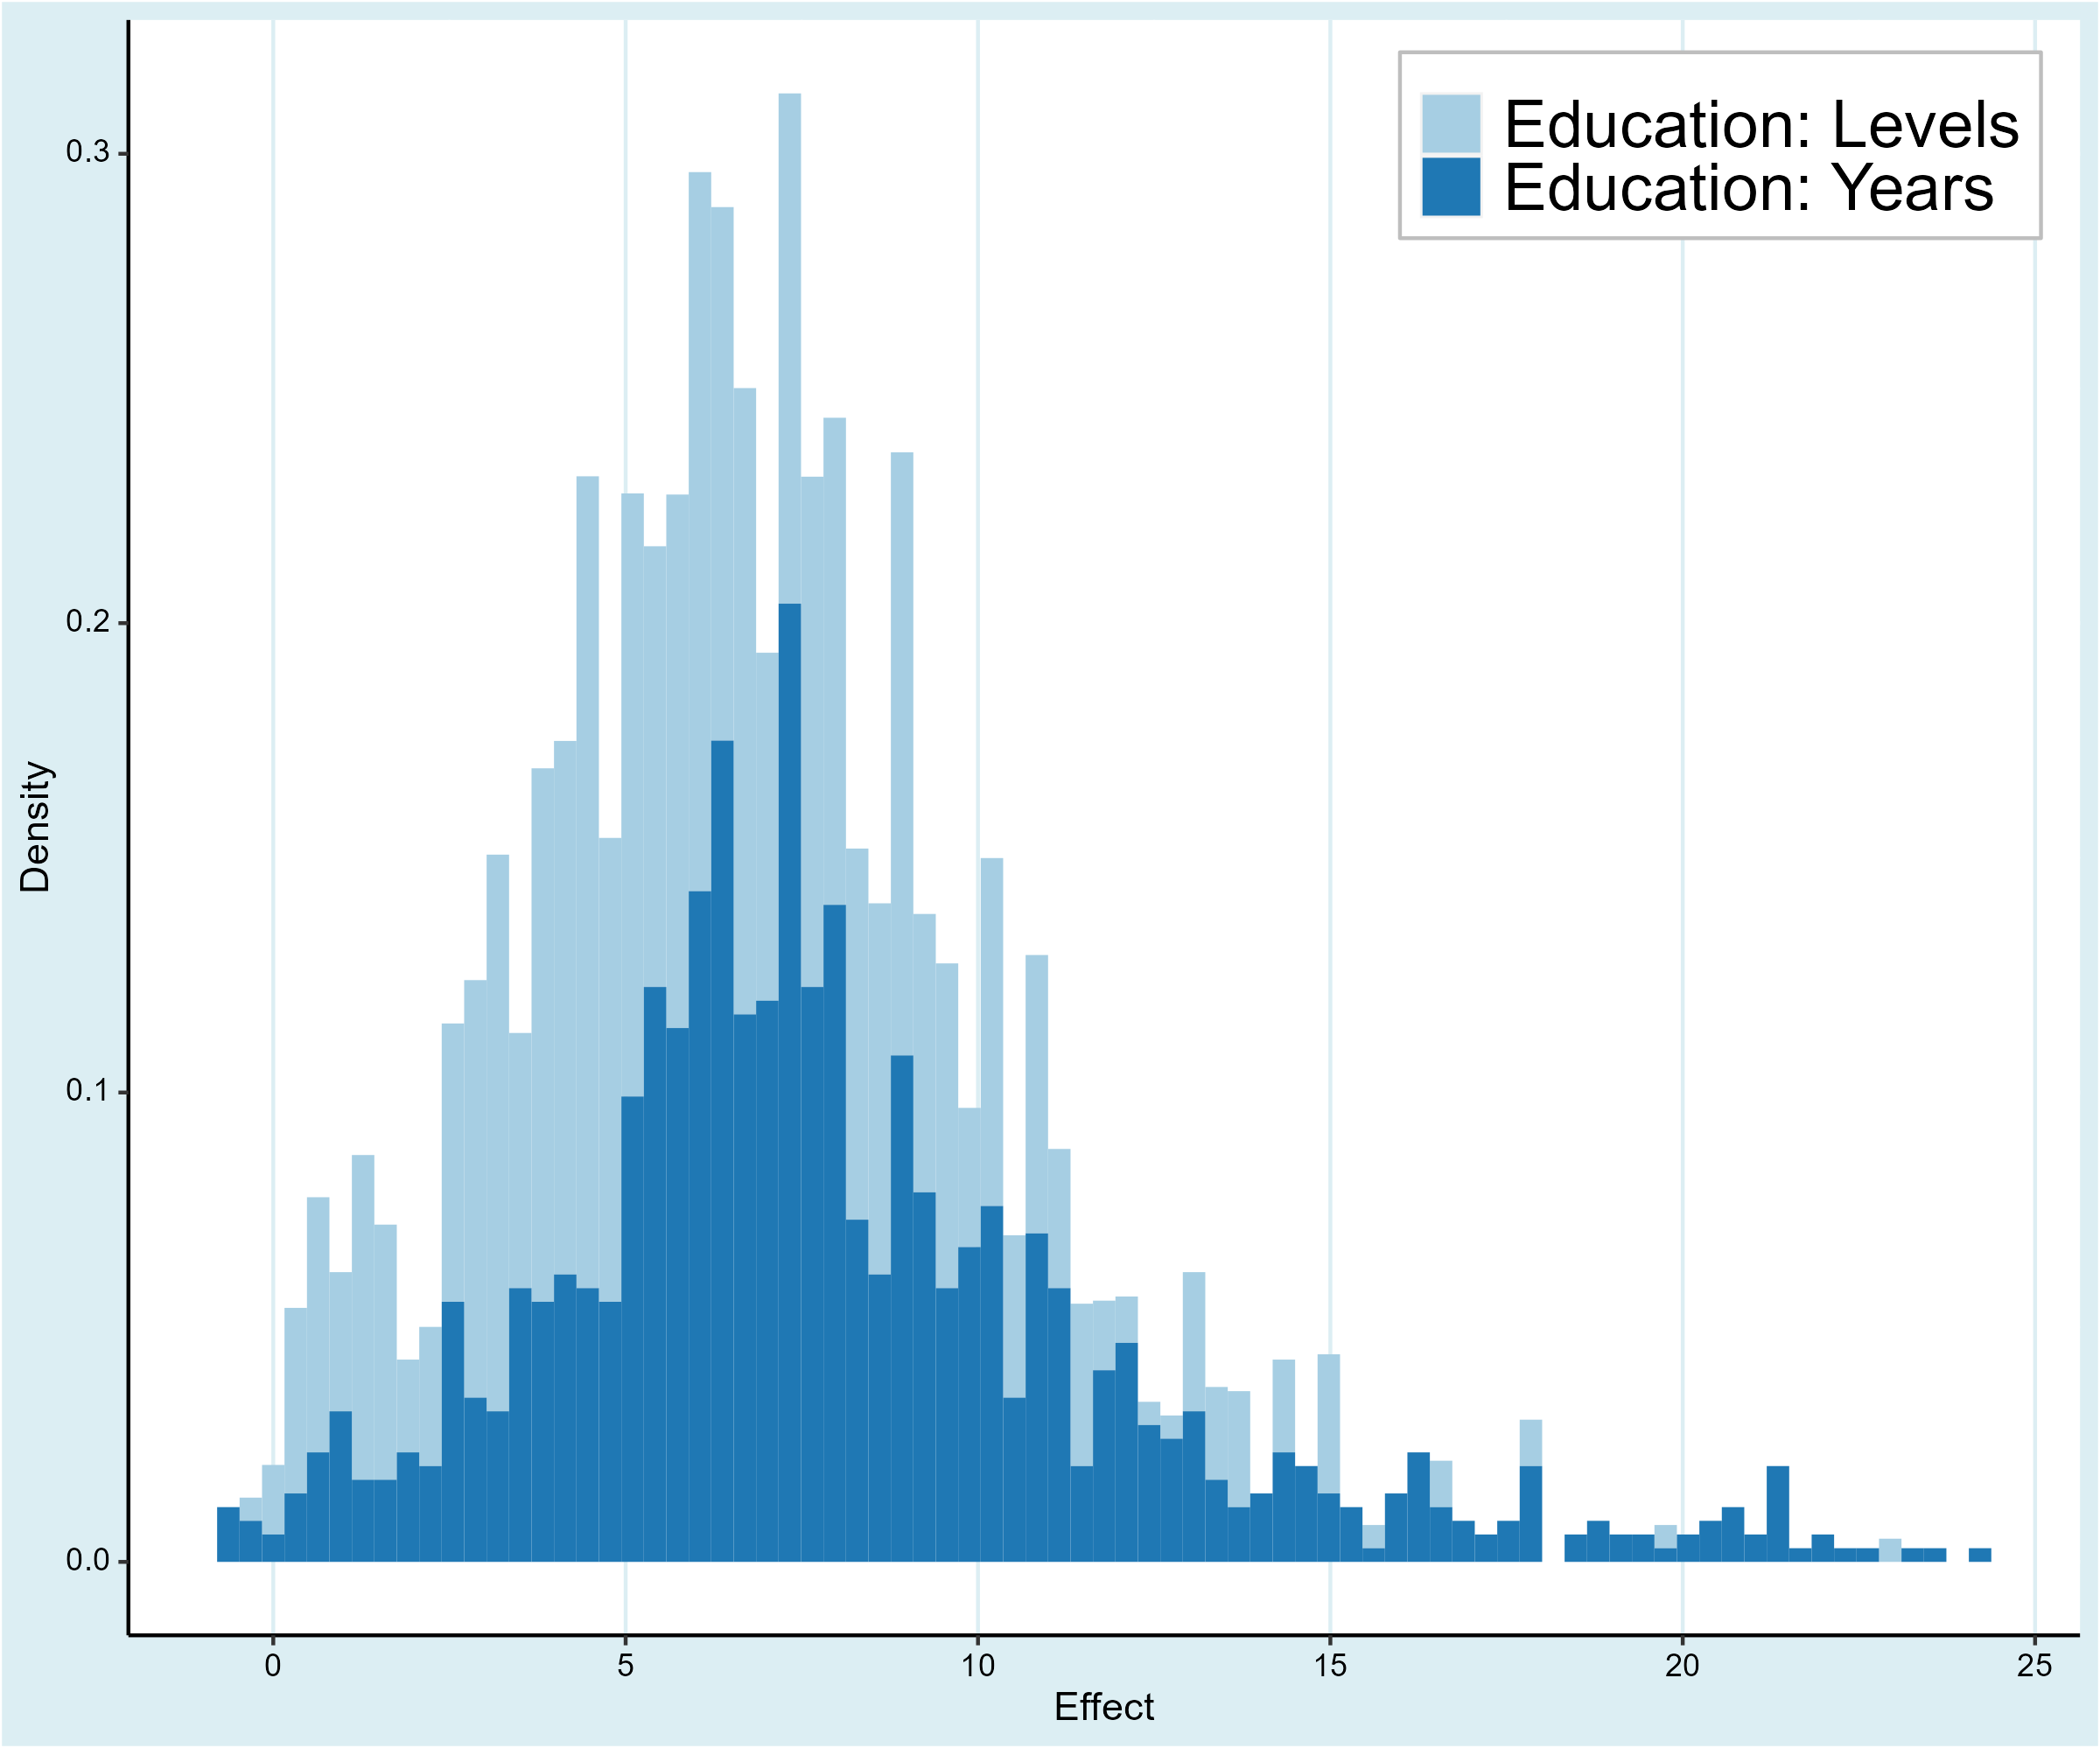
\includegraphics[width=0.95\linewidth]{Figures/Prima Facie/prima_facie_years_levels.png}
   \label{fig:prima_facie_years_levels}
\end{subfigure}
\begin{subfigure}[!htbp]{0.38\textwidth}
   \vspace{-0.1cm}
   \caption{Data type}
   \vspace{-0.1cm}
   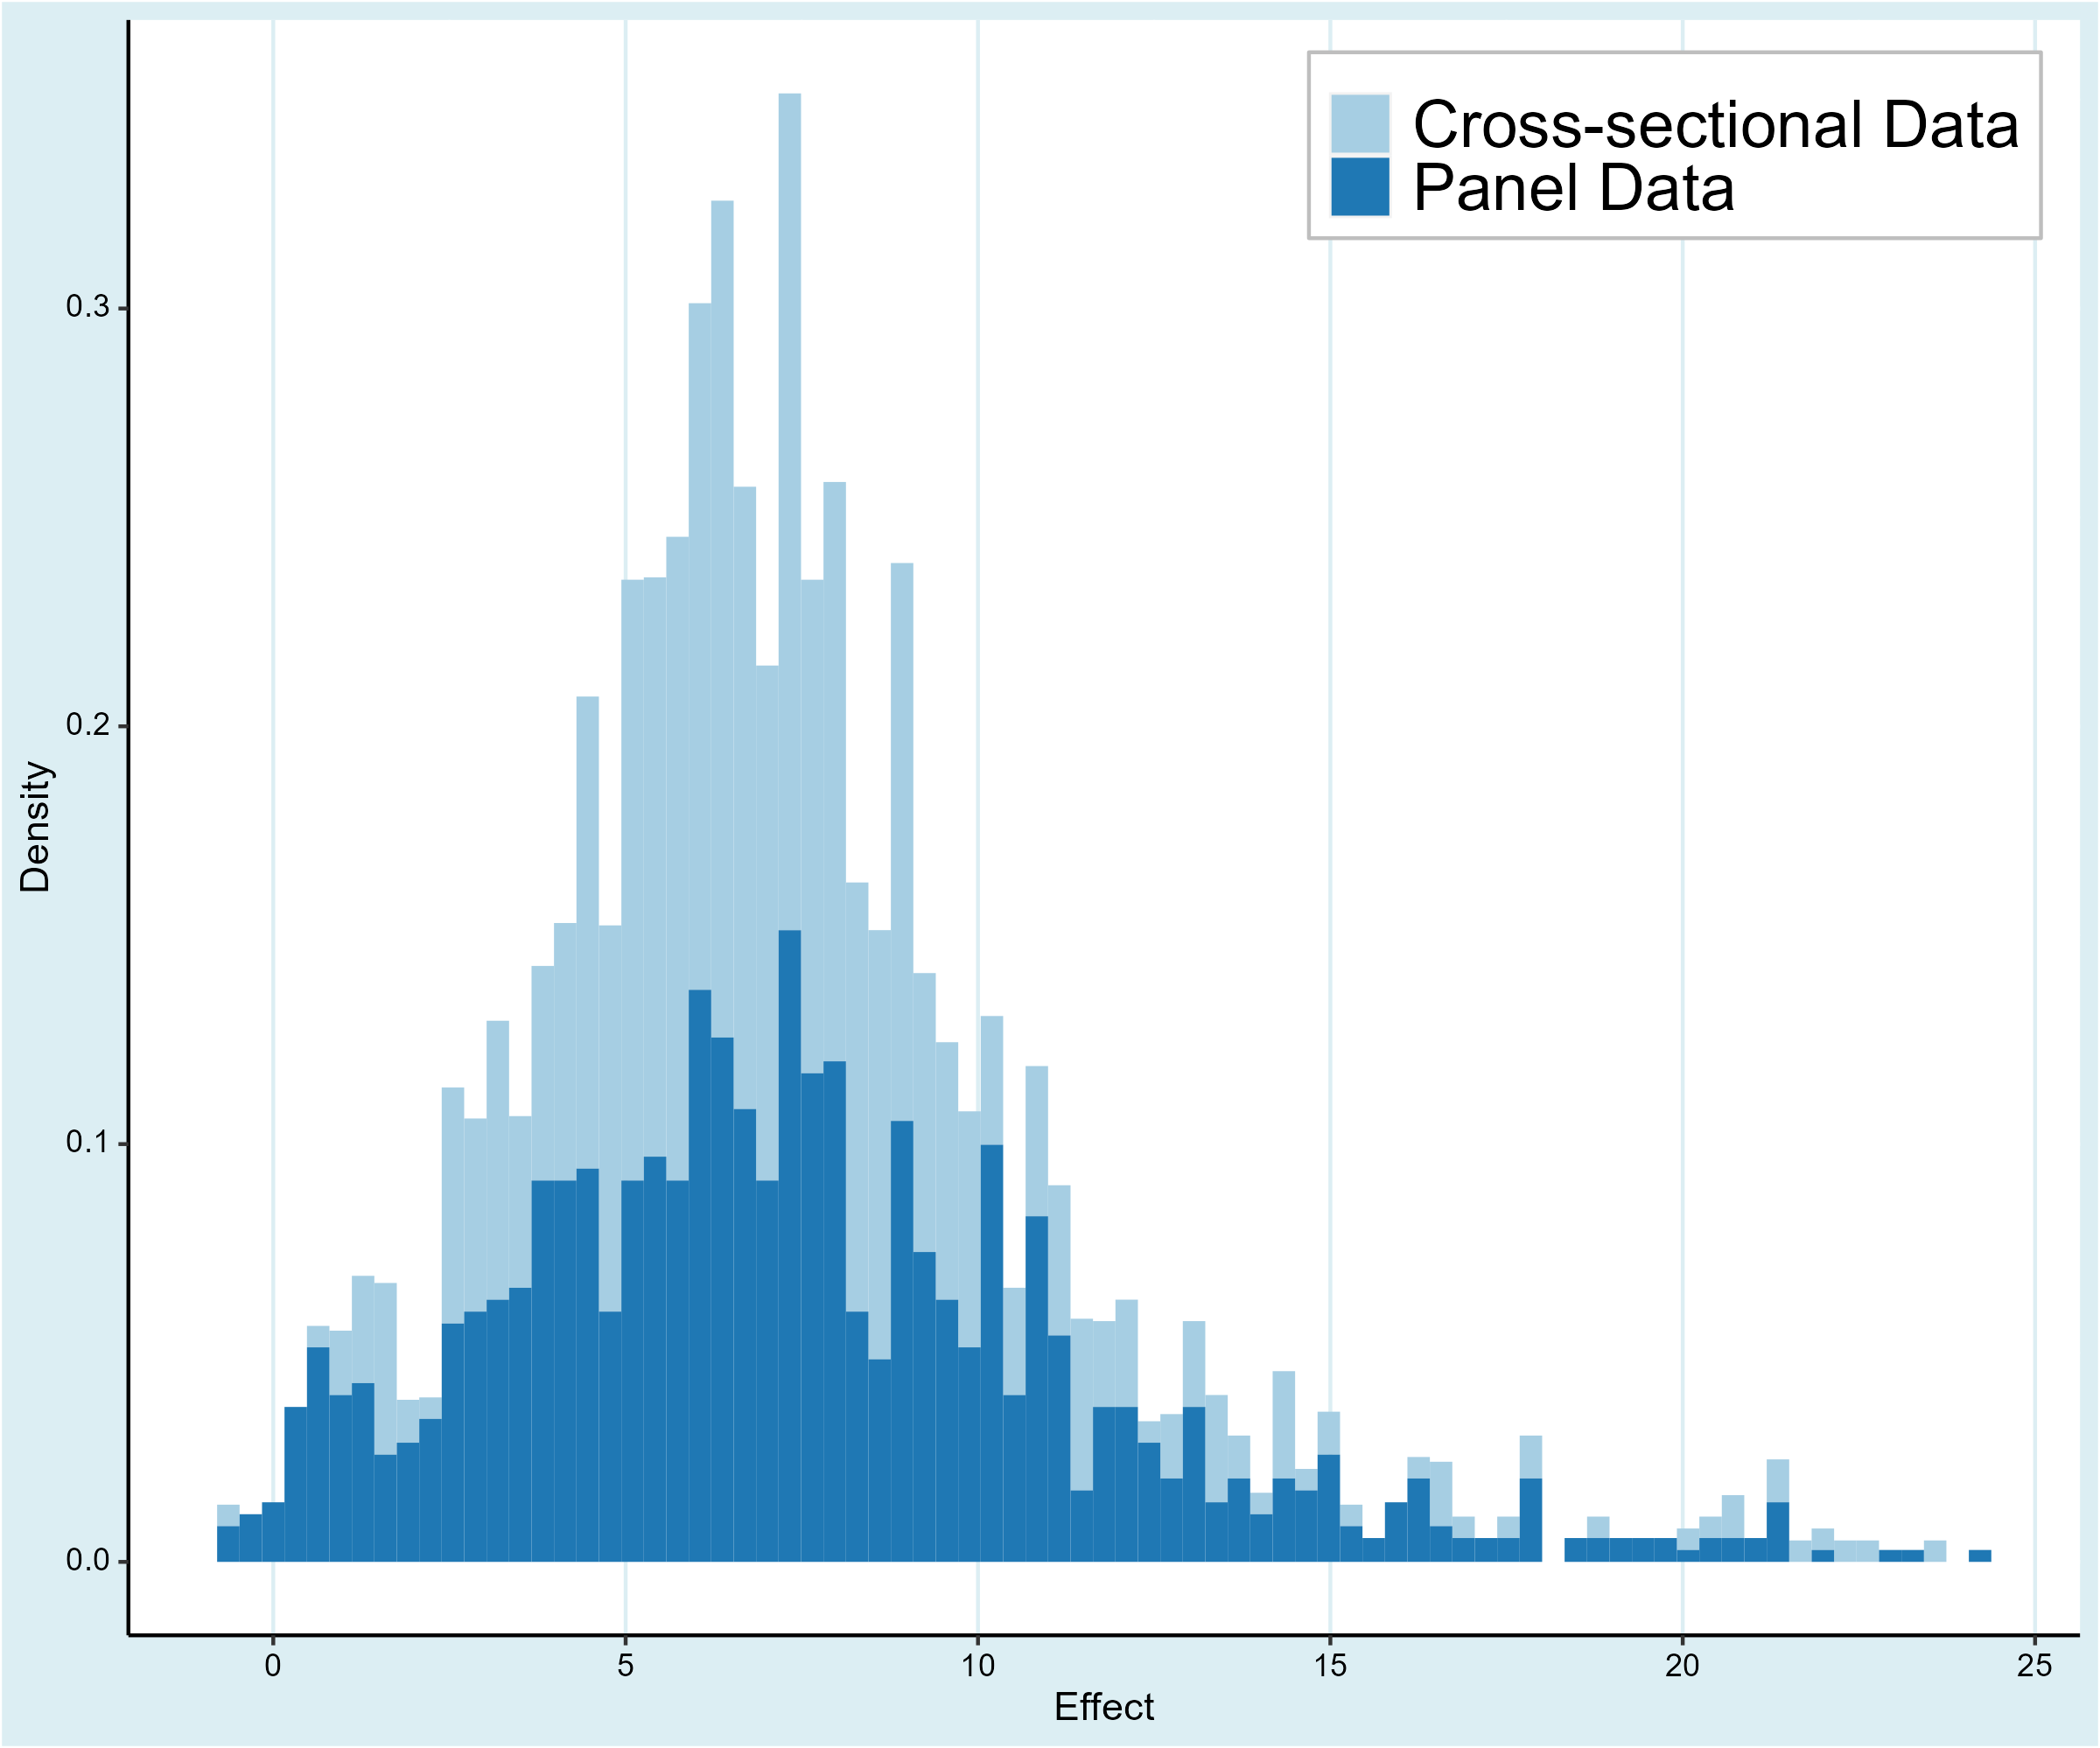
\includegraphics[width=0.95\linewidth]{Figures/Prima Facie/prima_facie_data_type.png}
   \label{fig:prima_facie_data_type}
\end{subfigure}

\begin{subfigure}[!htbp]{0.38\textwidth}
   \vspace{0.2cm}
   \caption{Highest education}
   \vspace{-0.1cm}
   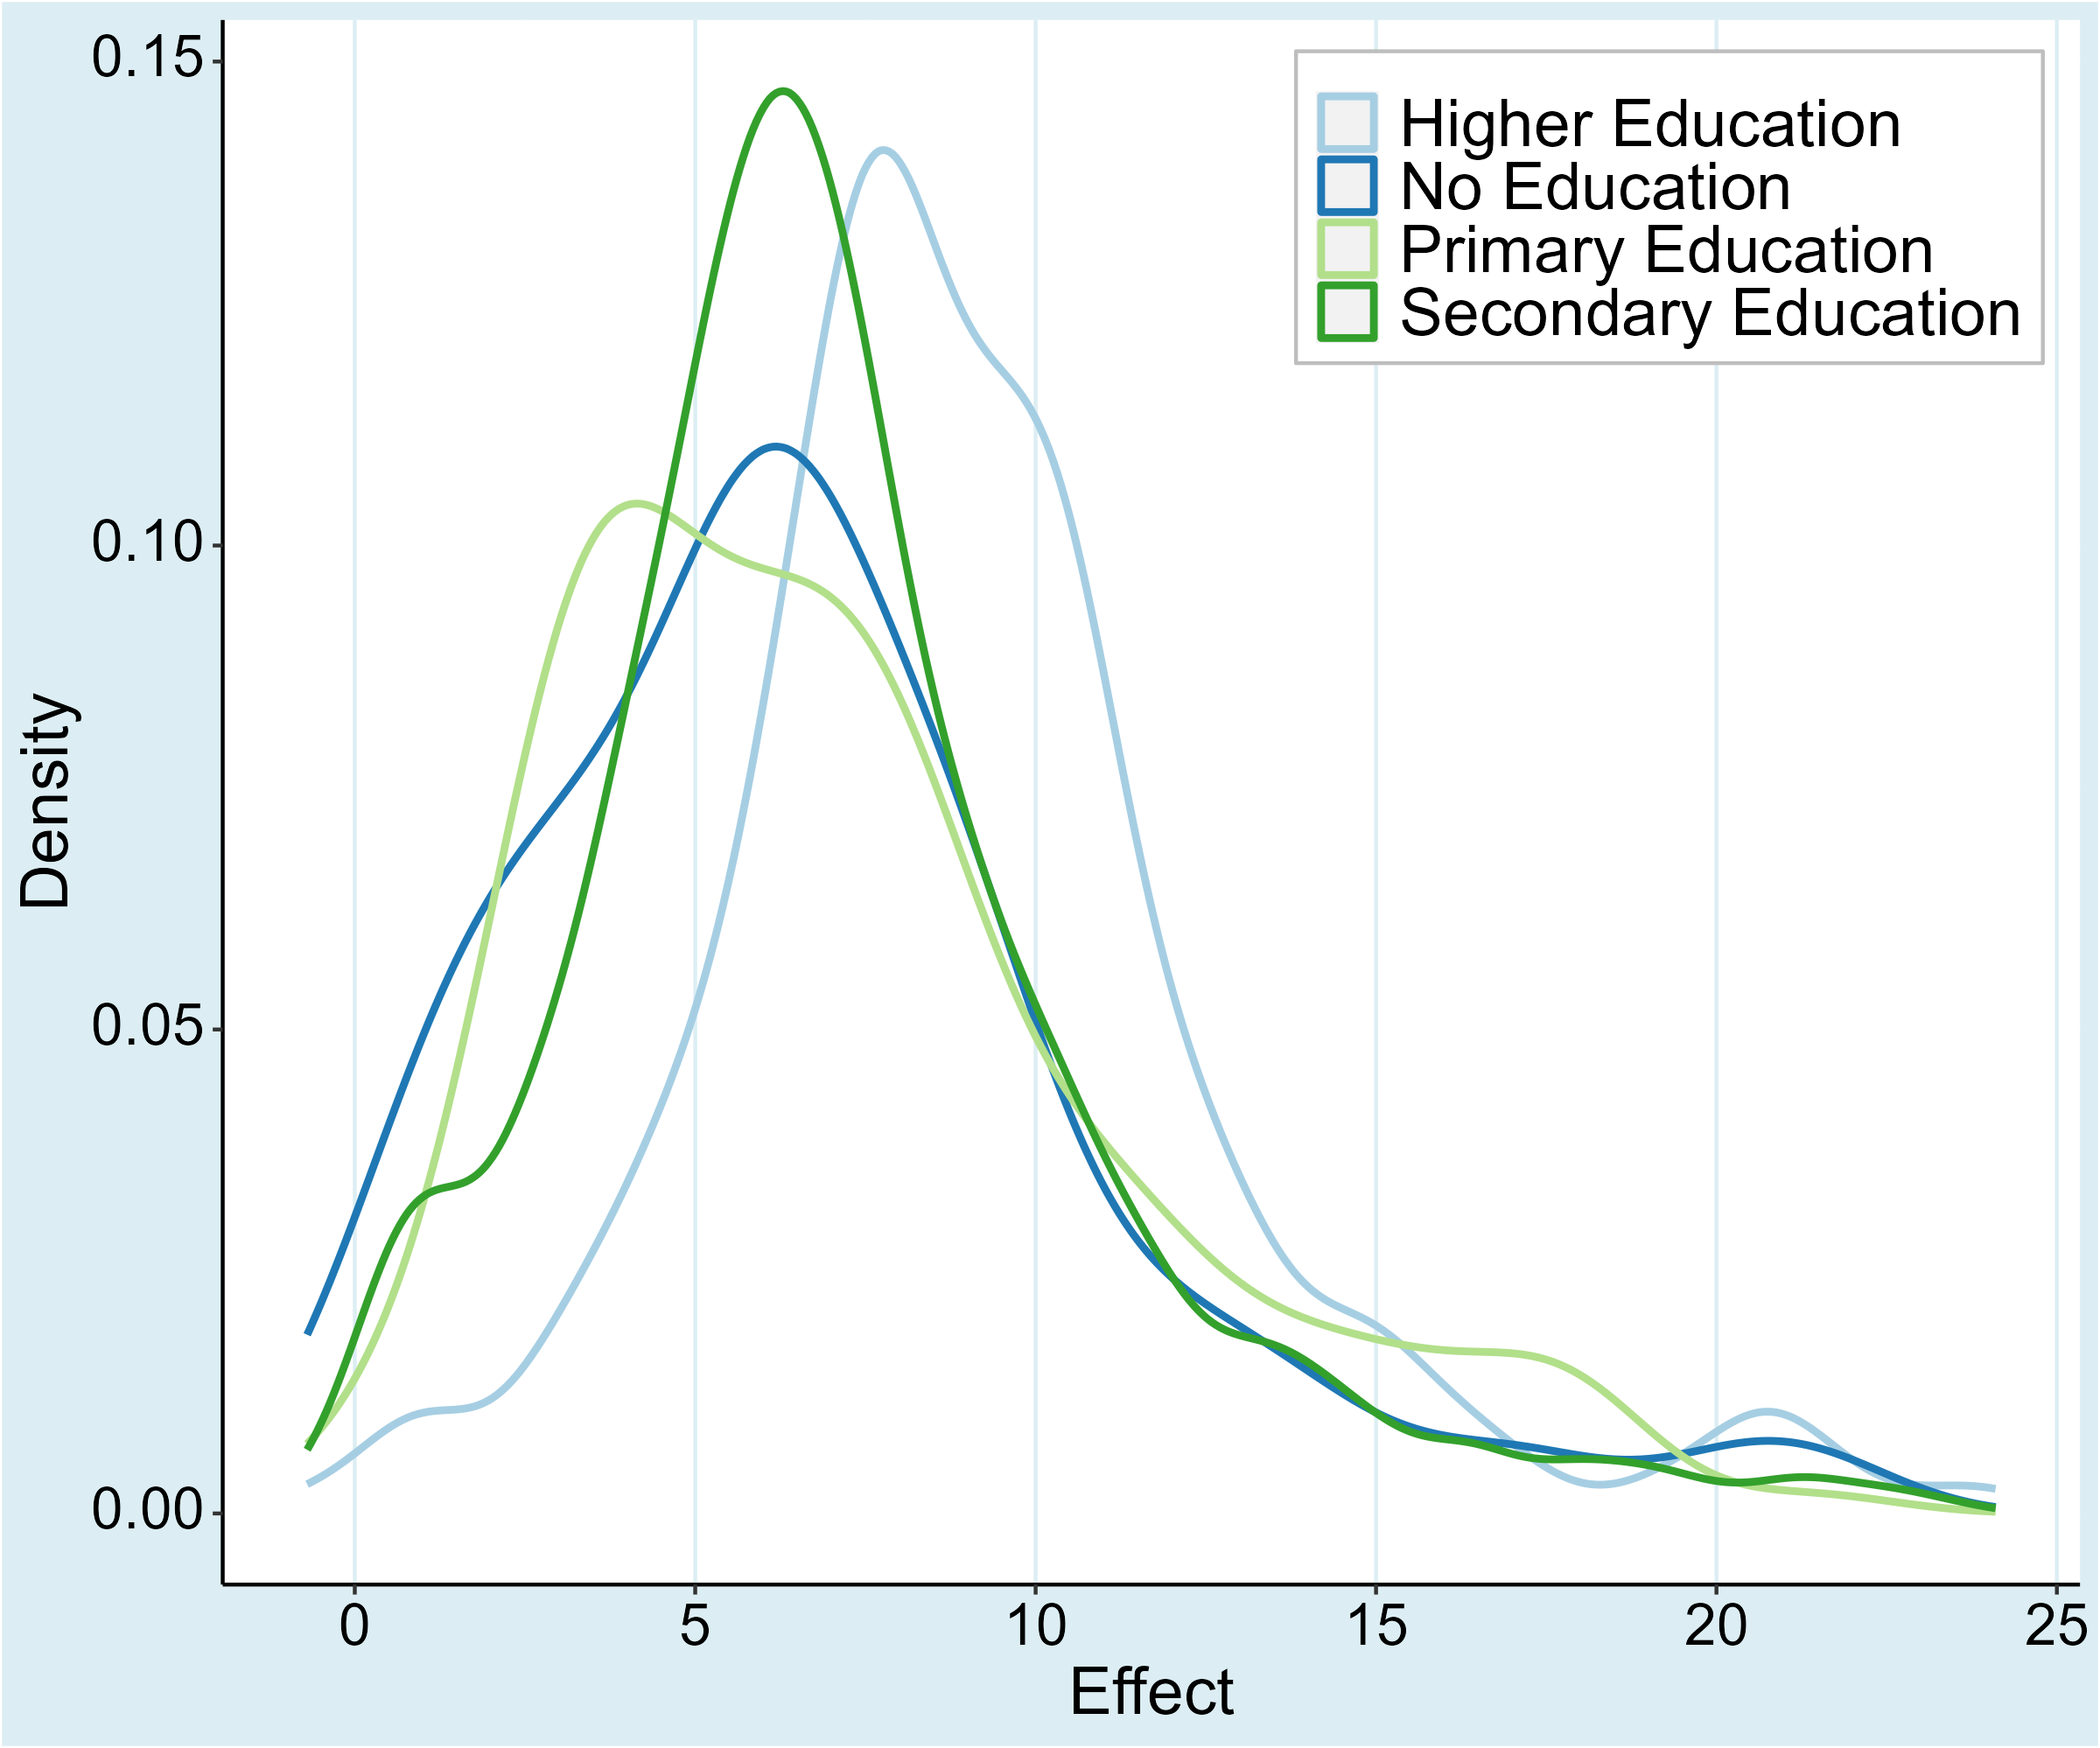
\includegraphics[width=0.95\linewidth]{Figures/Prima Facie/prima_facie_education.png}
   \label{fig:prima_facie_education}
\end{subfigure}
\begin{subfigure}[!htbp]{0.38\textwidth}
   \vspace{0.2cm}
   \caption{Gender}
   \vspace{-0.1cm}
   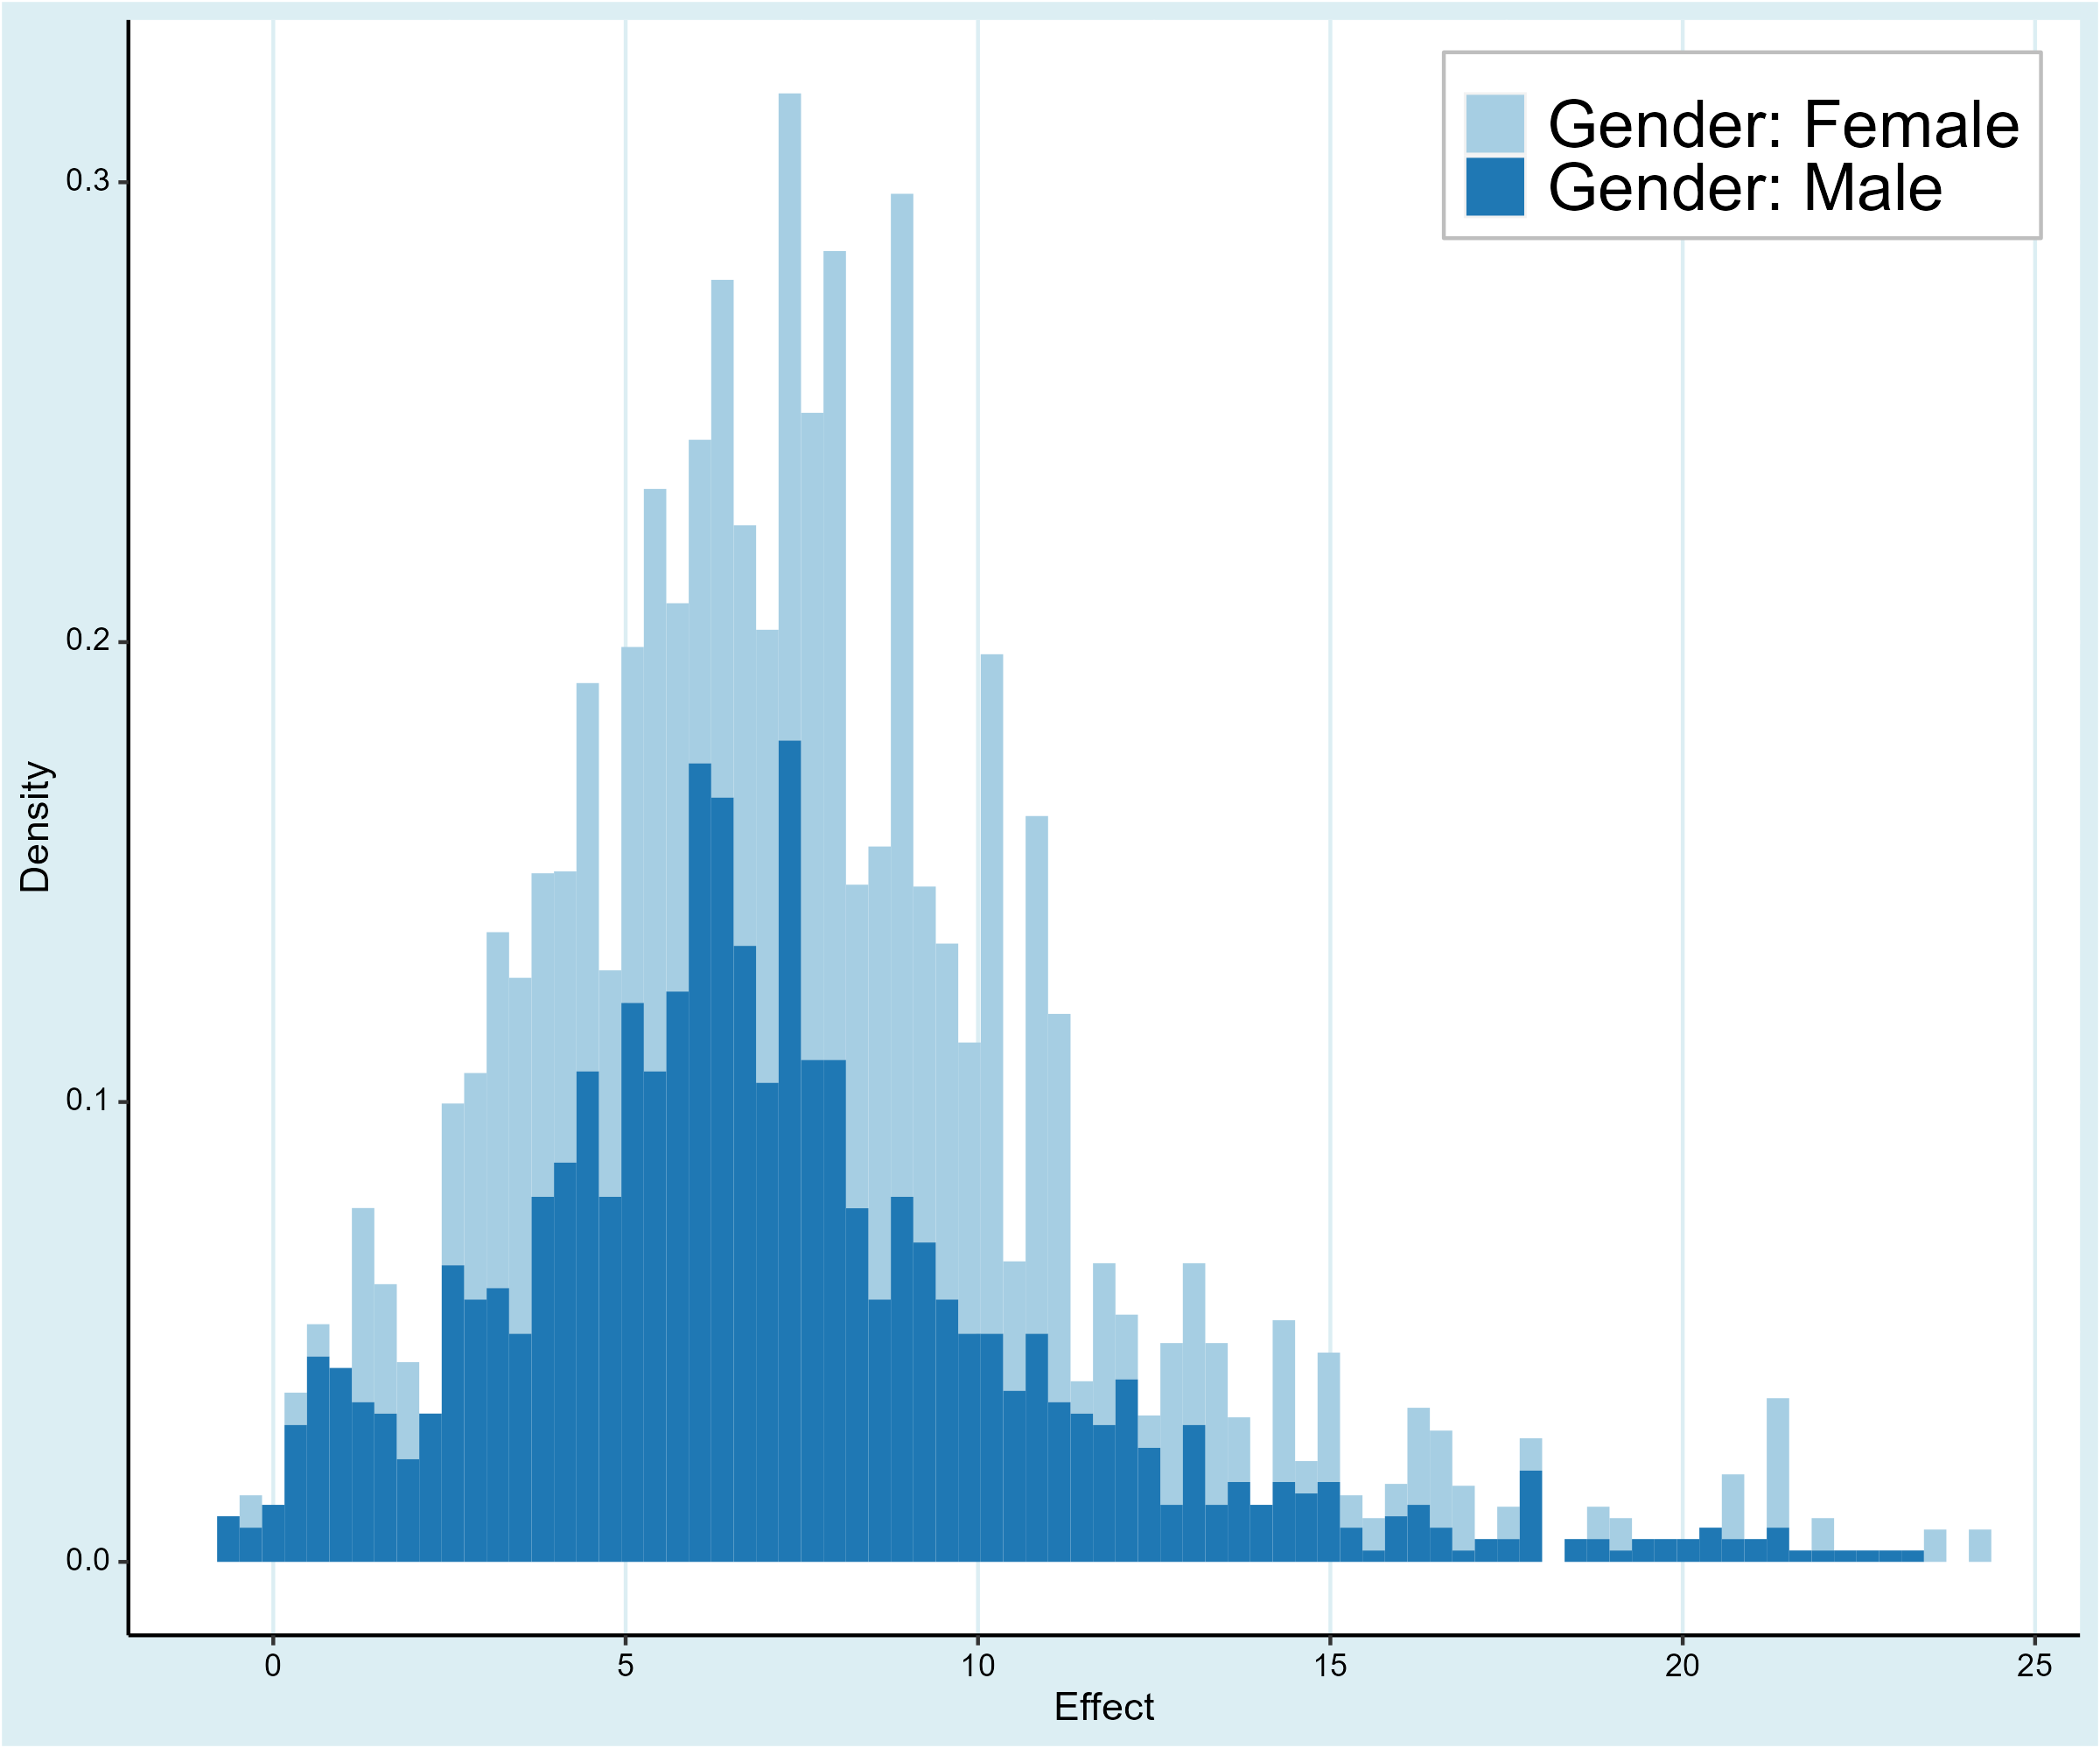
\includegraphics[width=0.95\linewidth]{Figures/Prima Facie/prima_facie_gender.png}
   \label{fig:prima_facie_gender}
\end{subfigure}

\begin{subfigure}[!htbp]{0.38\textwidth}
   \vspace{0.2cm}
   \caption{Country wealth}
   \vspace{-0.1cm}
   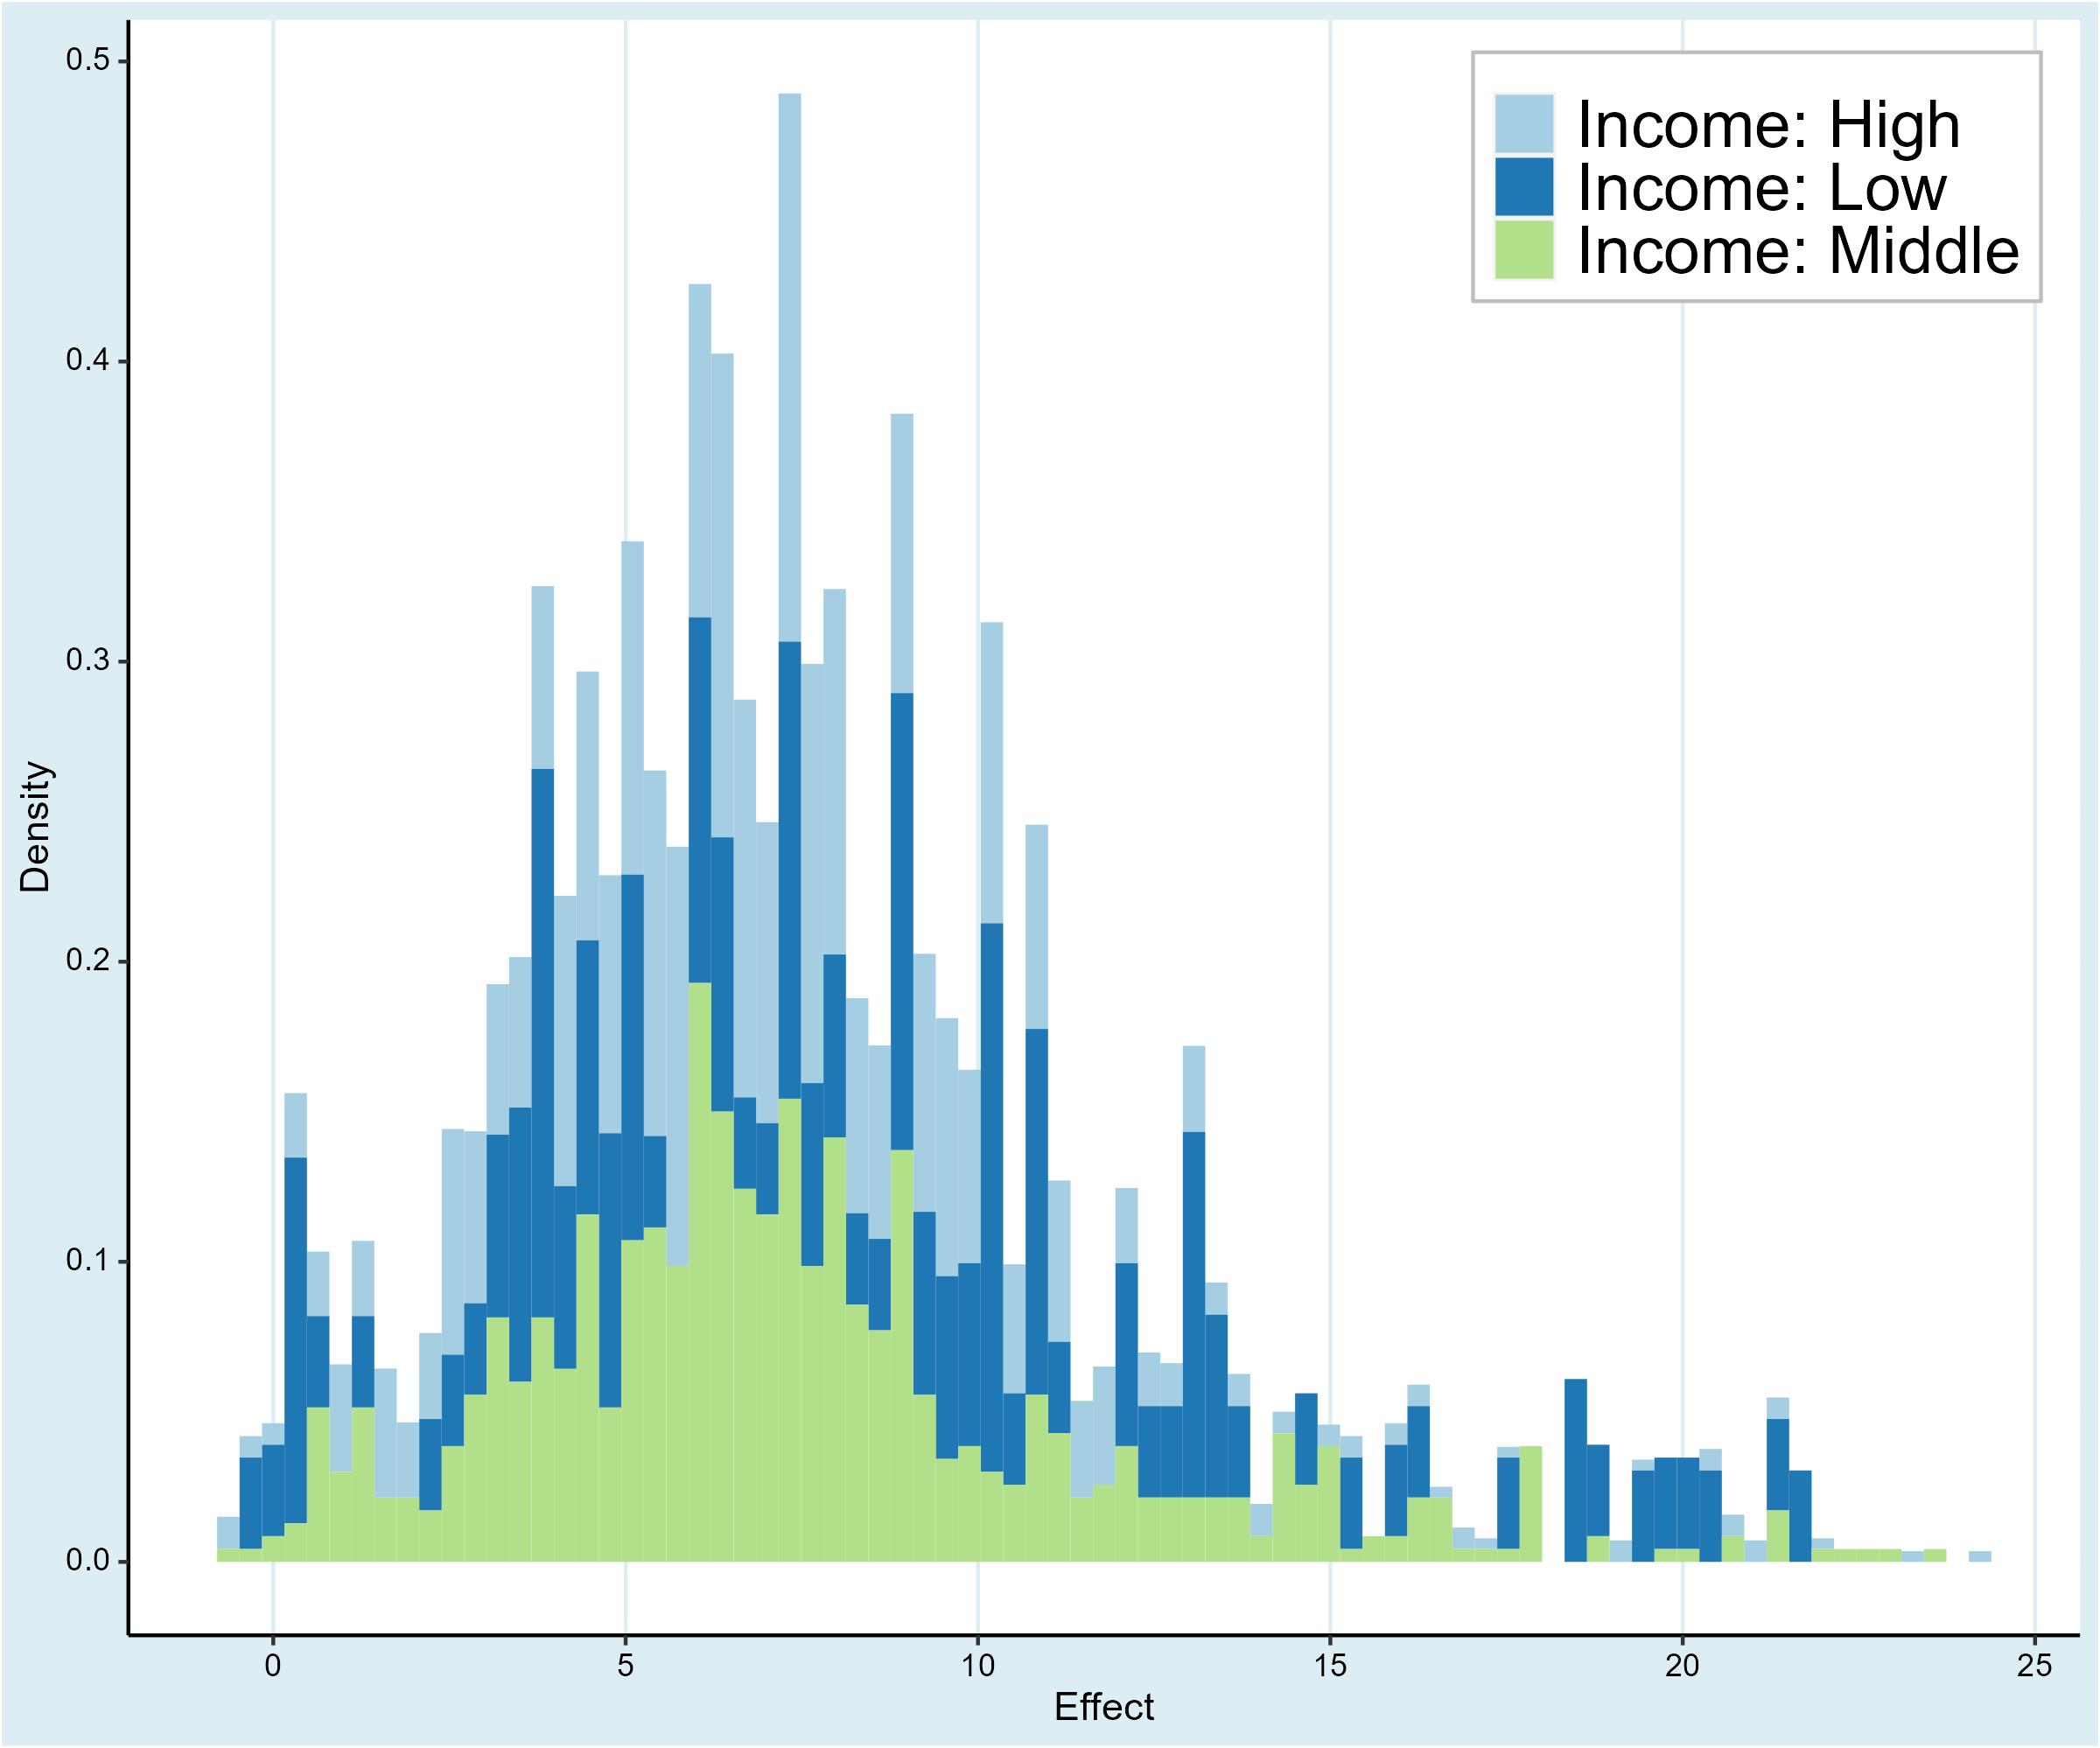
\includegraphics[width=0.95\linewidth]{Figures/Prima Facie/prima_facie_income.png}
   \label{fig:prima_facie_income}
\end{subfigure}
\begin{subfigure}[!htbp]{0.38\textwidth}
   \vspace{0.2cm}
   \caption{Estimation method}
   \vspace{-0.1cm}
   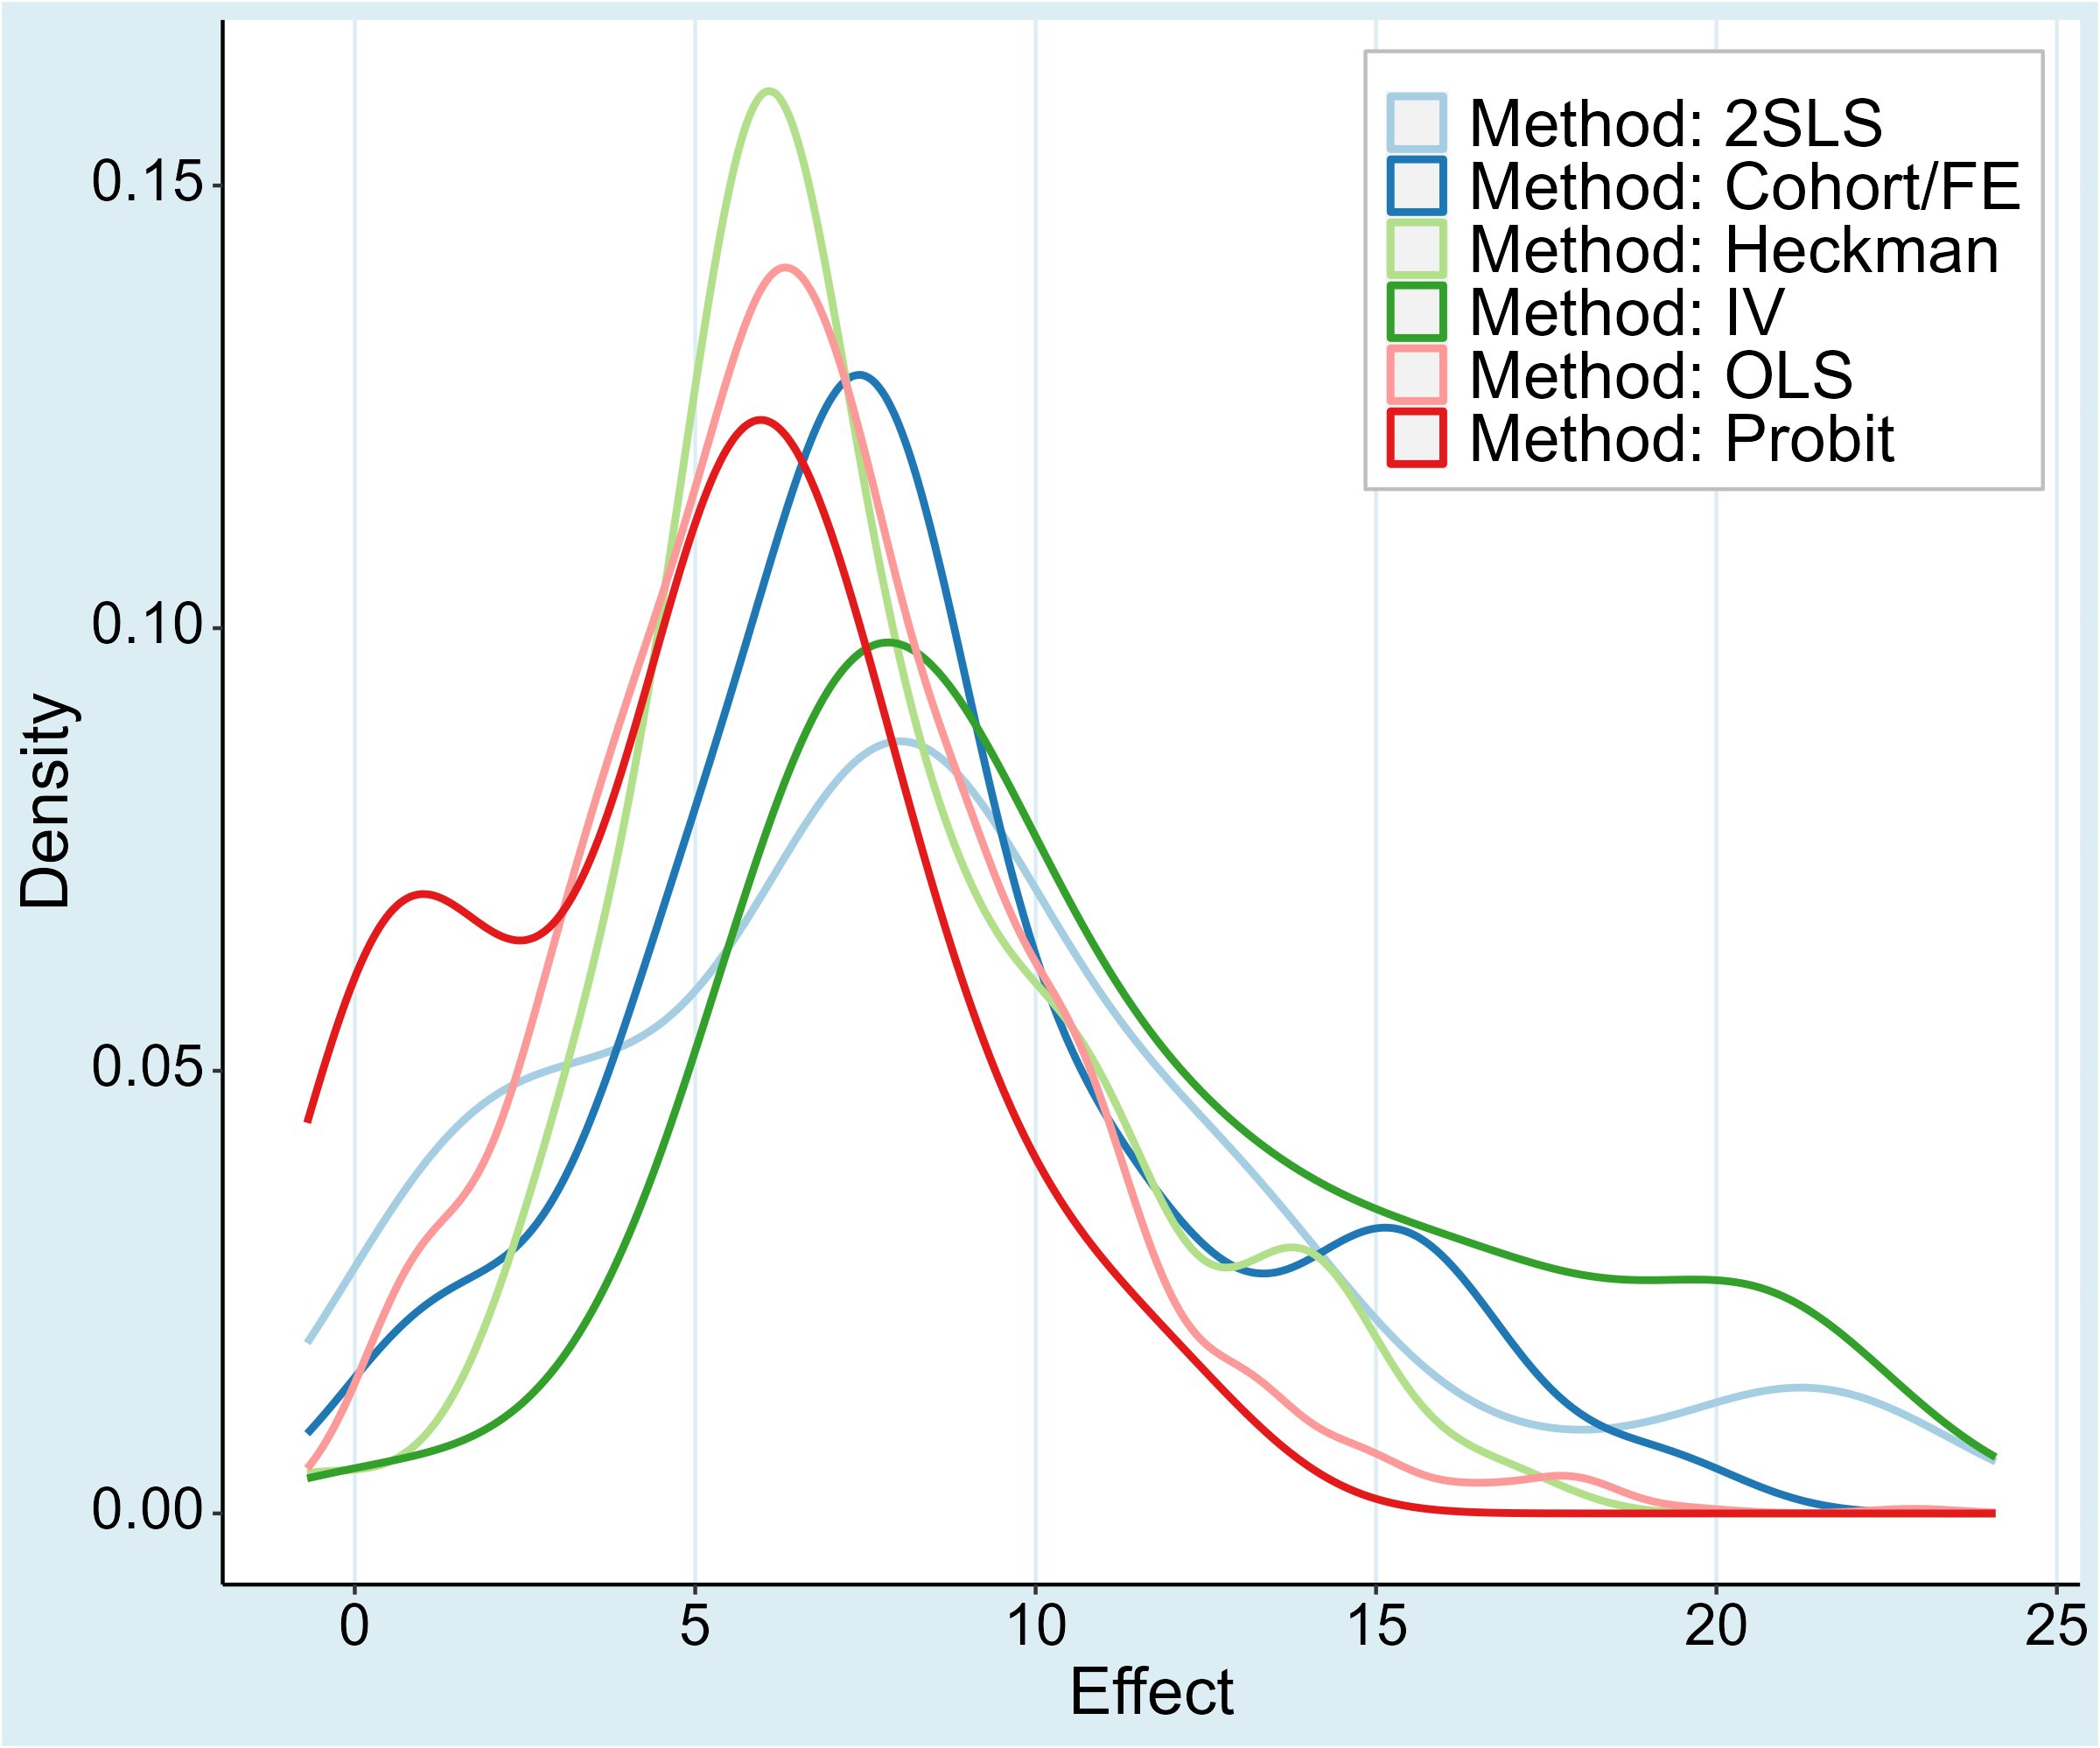
\includegraphics[width=0.95\linewidth]{Figures/Prima Facie/prima_facie_method.png}
   \label{fig:prima_facie_method} 
\end{subfigure}

\begin{subfigure}[!htbp]{0.38\textwidth}
   \vspace{0.2cm}
   \caption{Ability}
   \vspace{-0.1cm}
   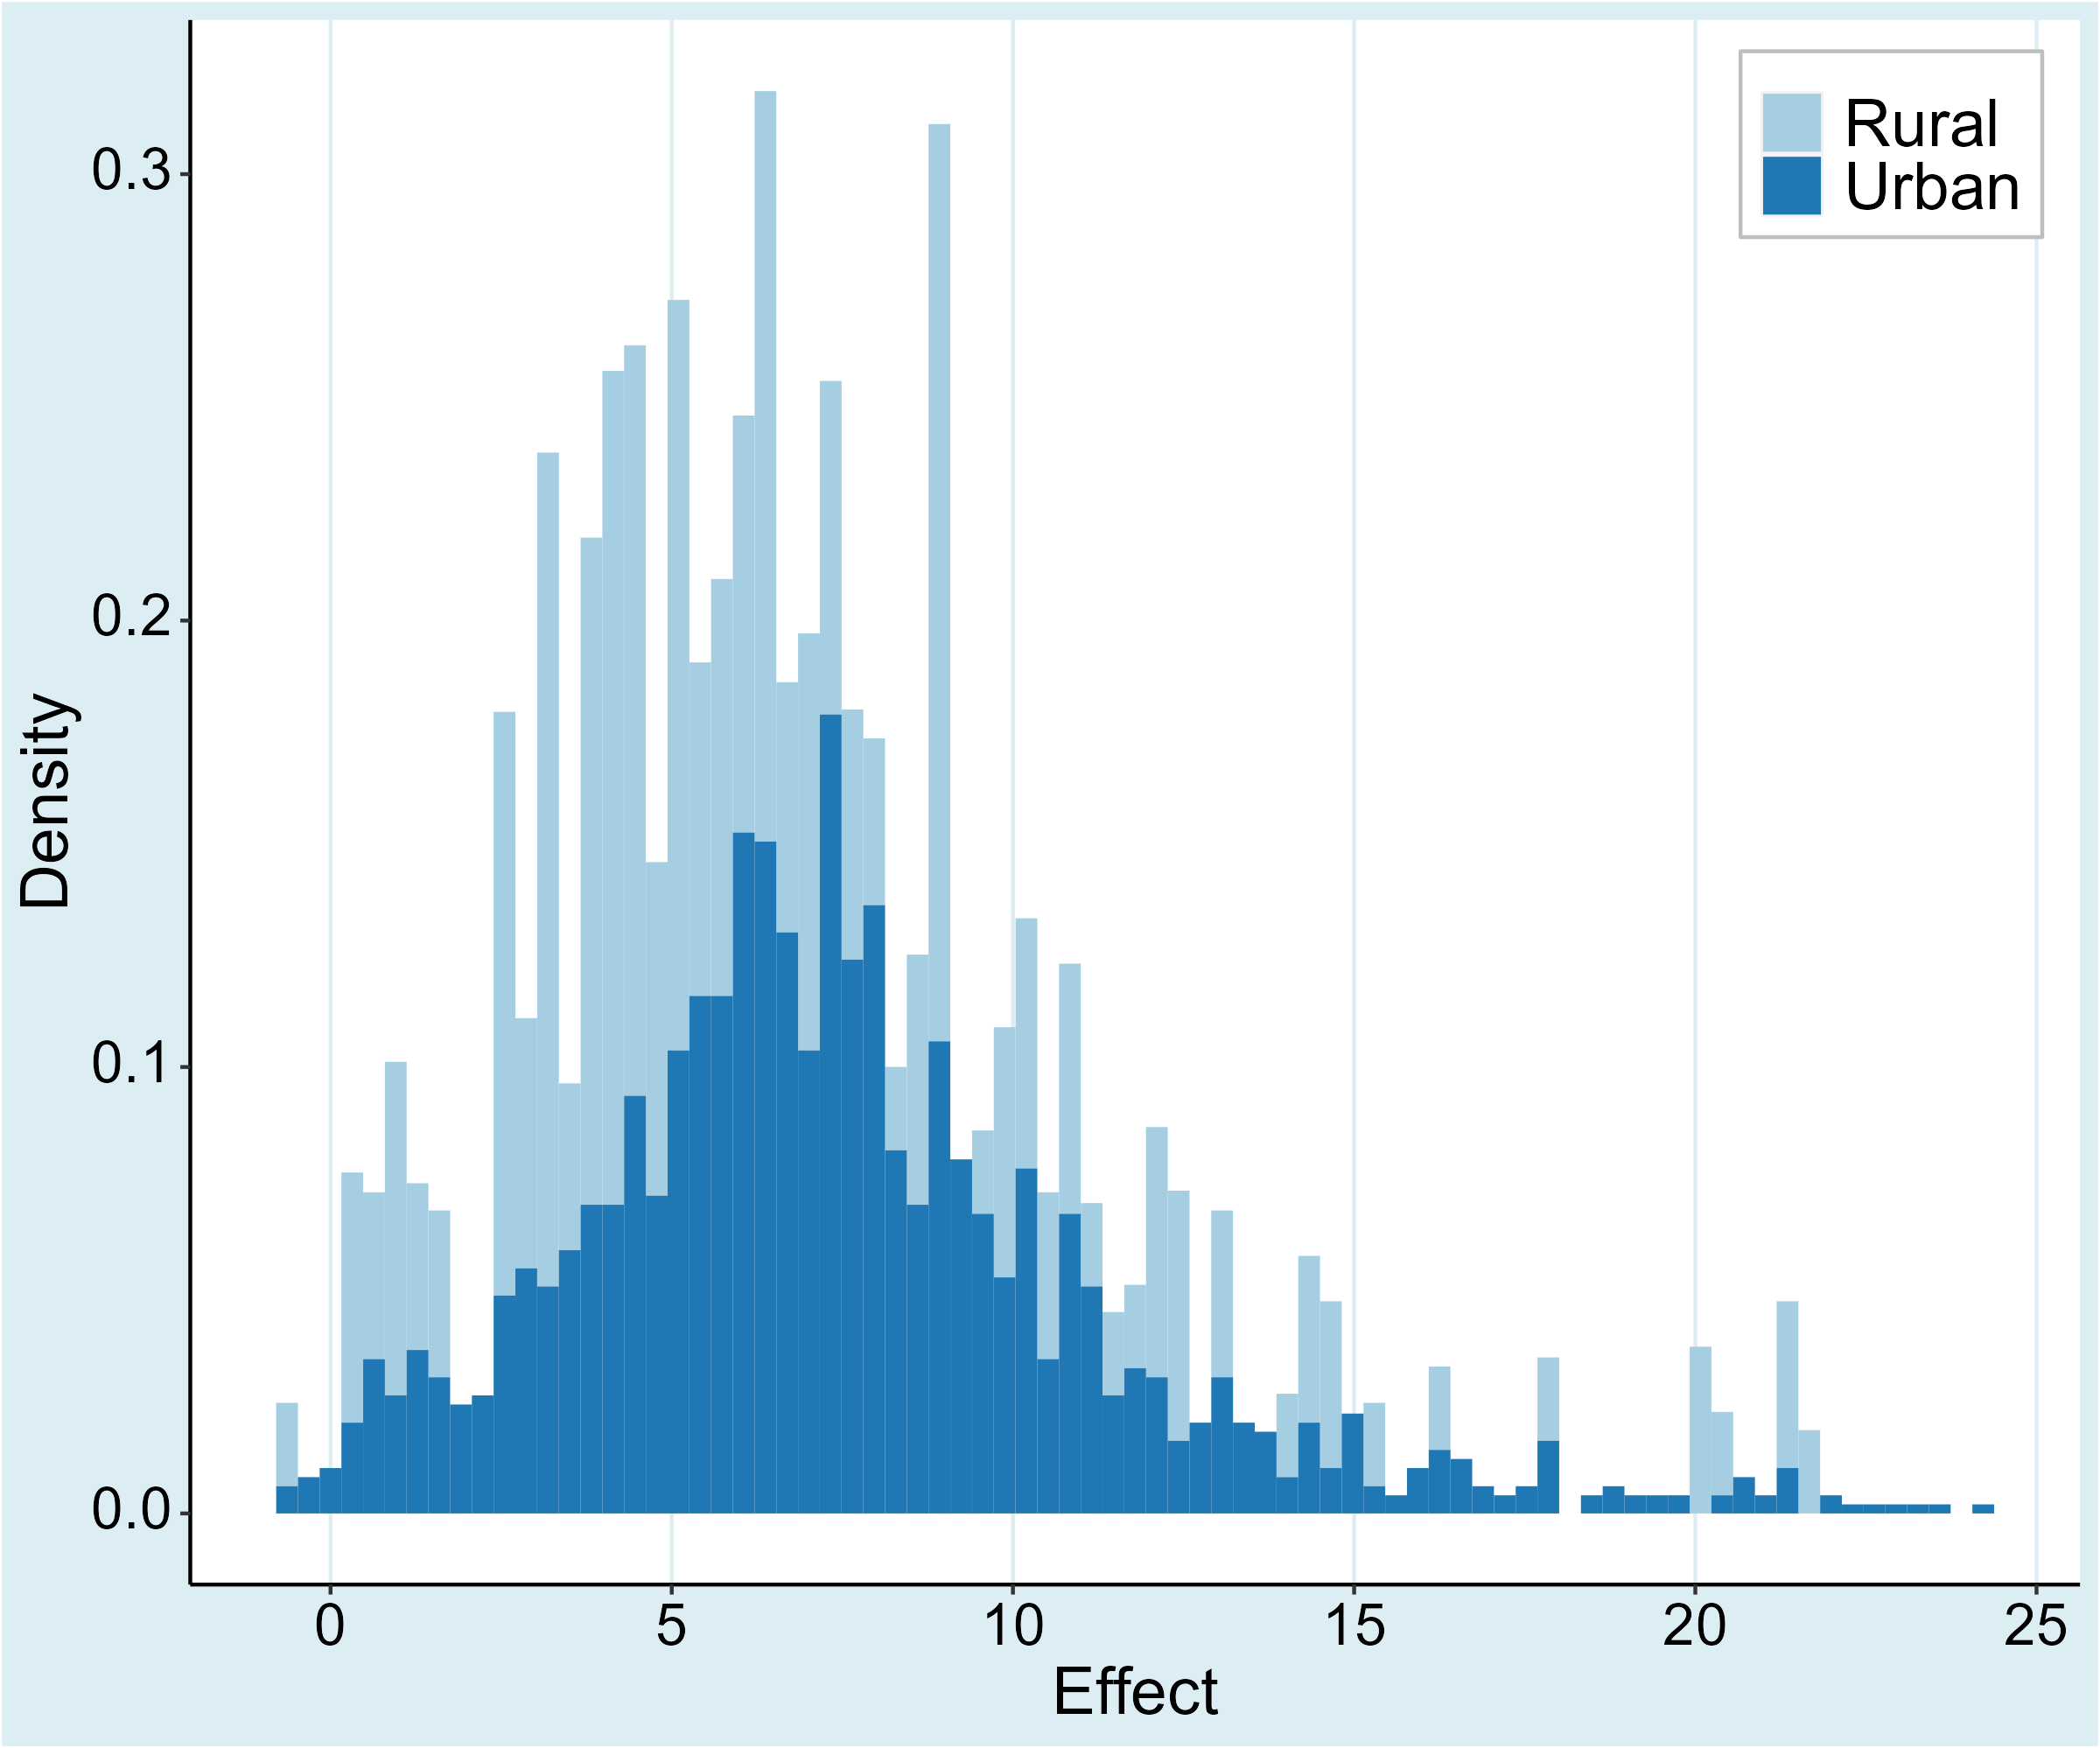
\includegraphics[width=0.95\linewidth]{Figures/Prima Facie/prima_facie_ability.png}
   \label{fig:prima_facie_ability}
\end{subfigure}
\begin{subfigure}[!htbp]{0.38\textwidth}
   \vspace{0.2cm}
   \caption{Citations}
   \vspace{-0.1cm}
   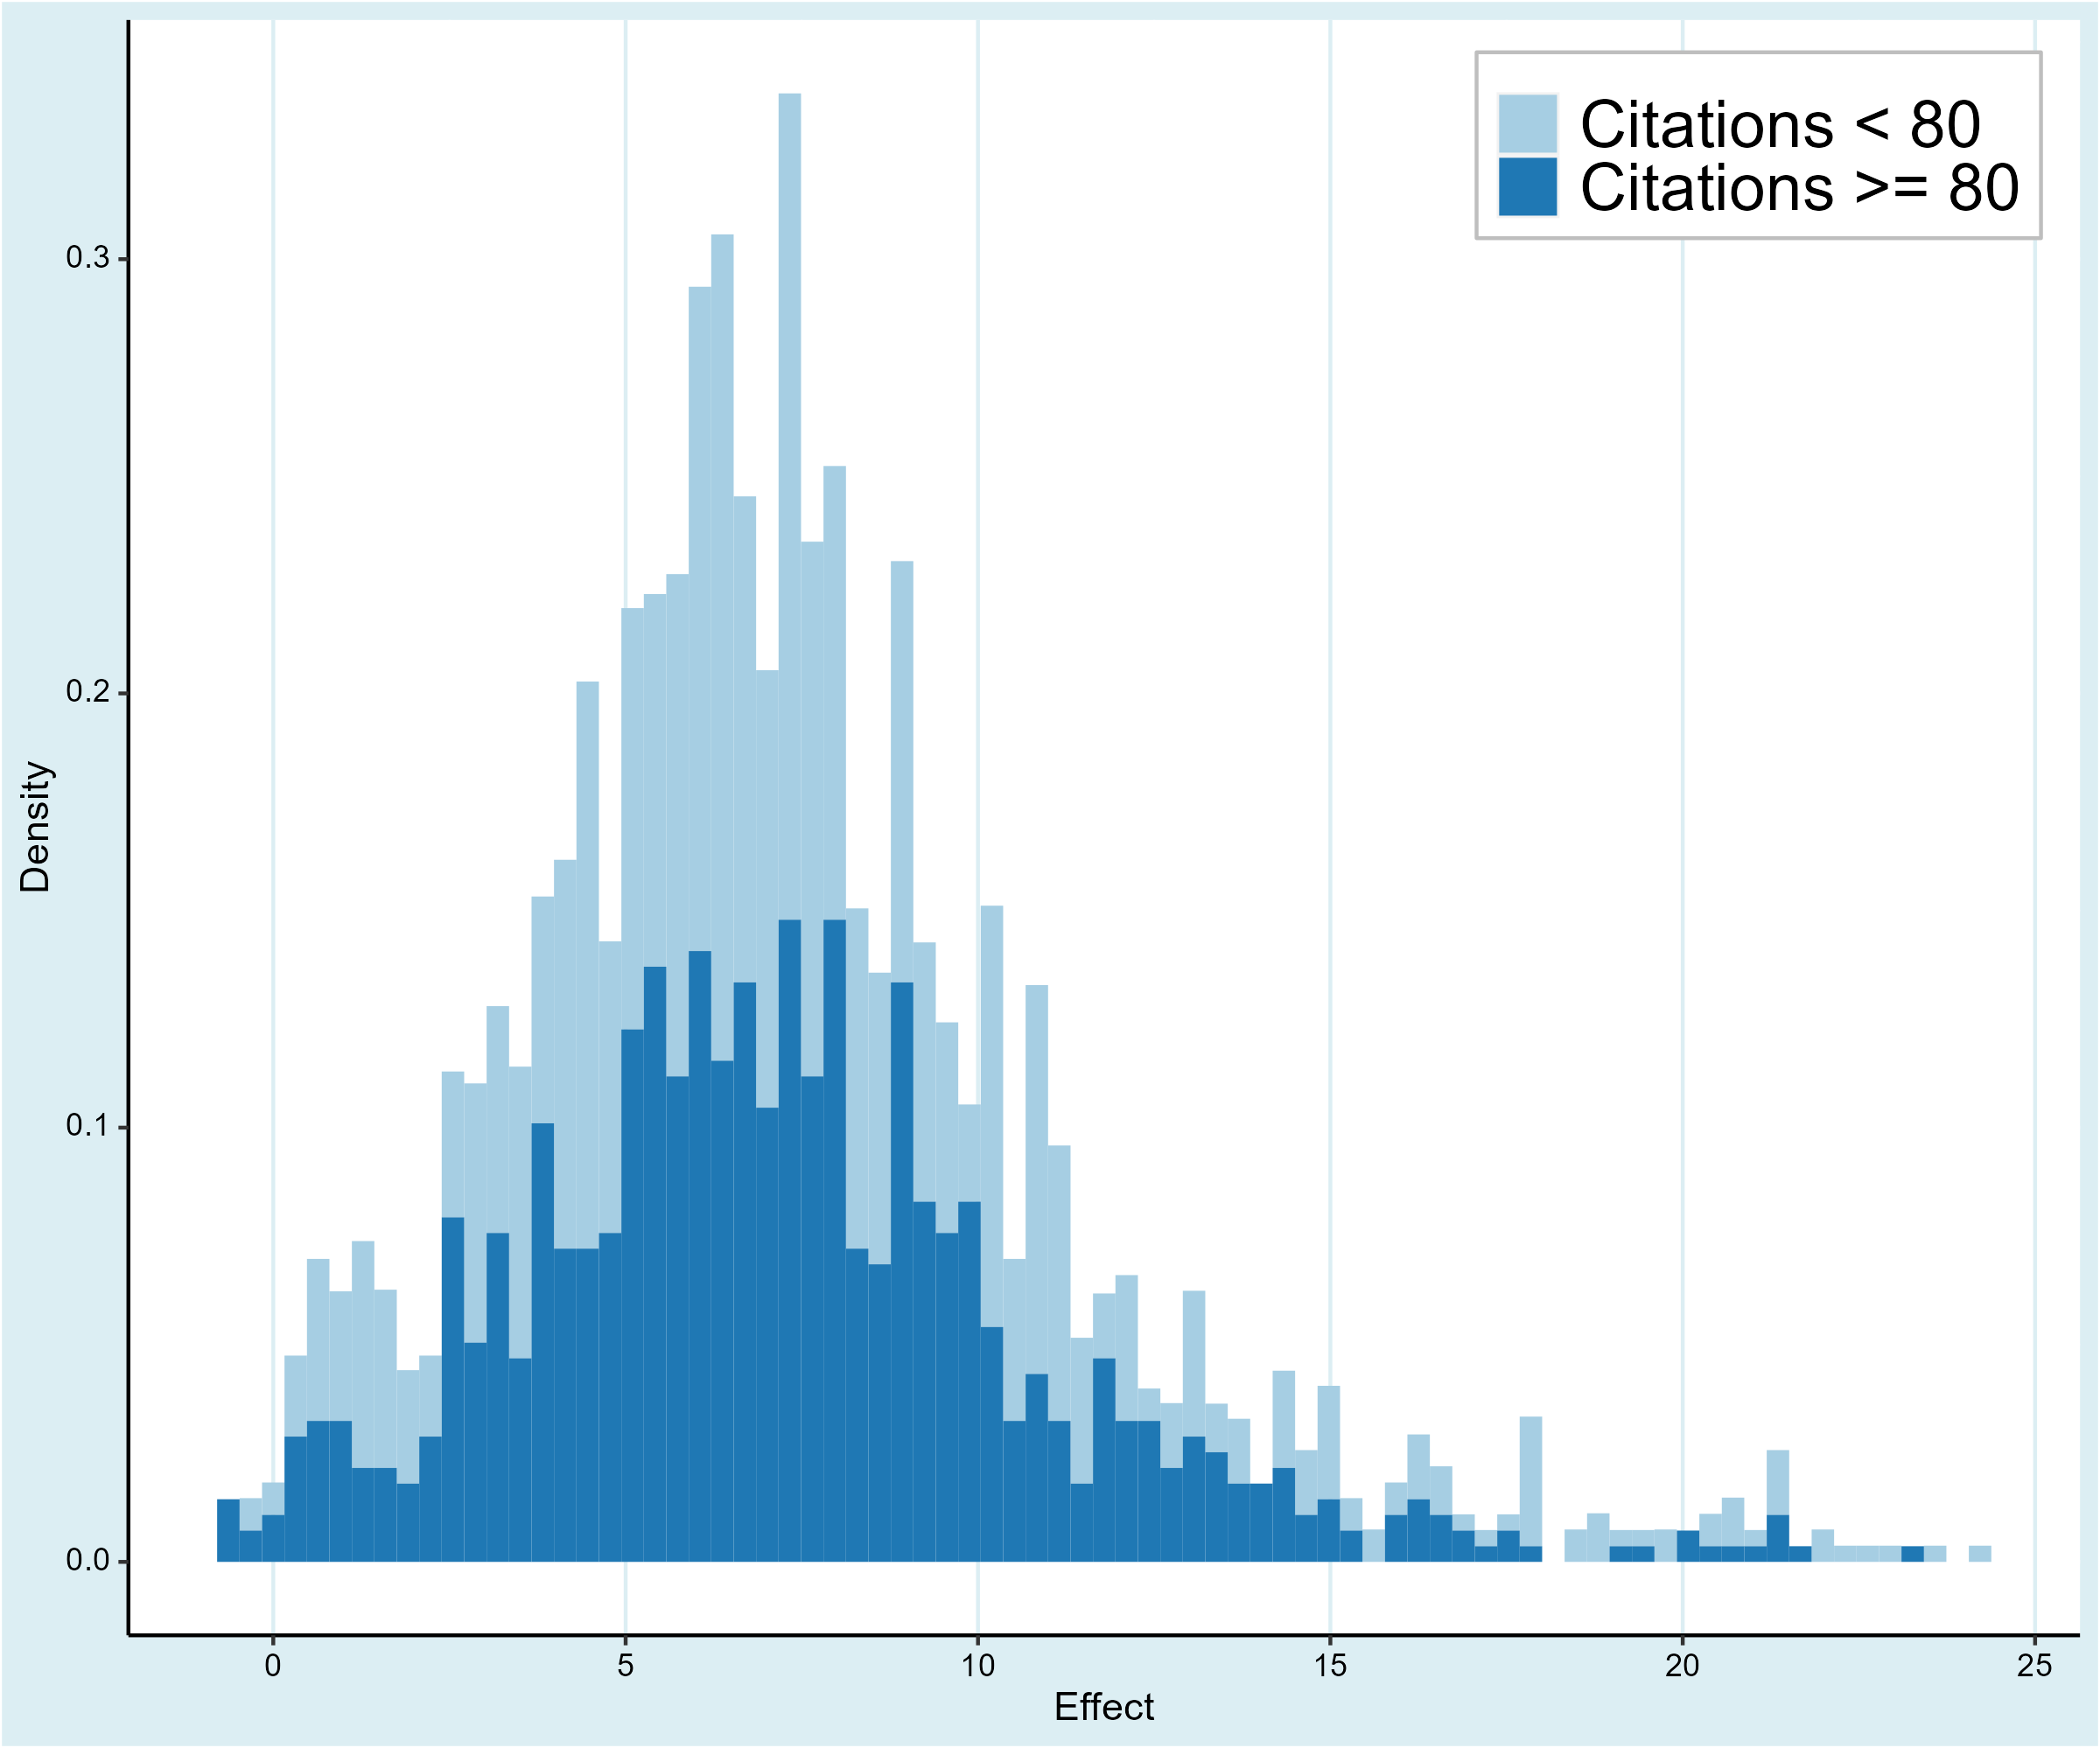
\includegraphics[width=0.95\linewidth]{Figures/Prima Facie/prima_facie_citations.png}
   \label{fig:prima_facie_citations}
\end{subfigure}

\end{center}\vspace{-0.6cm}
\captionsetup{width=0.75\textwidth, font = scriptsize}
\caption*{\emph{Note:} This figure displays histograms and density lines for different subsets of data, where the effect of an additional year of schooling on returns is displayed on the x-axis against its density on the y-axis. For \autoref{fig:prima_facie_citations}, the data median is used to determine the subsets. For a description of variables used in this figure, see \autoref{tab:var}.}
\end{figure}


First, I quickly address the numeric results. As a baseline for the rest of the work, we can observe that the unweighted mean of the effect across all data equals 7.476 (7.652 for the data weighted by the number of estimates reported per study). As a reminder, this can be interpreted as a 7.456\% increase in log wage per additional year of attained schooling and falls well into the expected range, comparing this estimate to the results of other works. As such, this brief insight can serve as a sanity check that there is nothing immediately wrong with the data collection. When comparing to individual studies, this mean is slightly lower than \cite{psacharopoulos2018meta} who claim about 9\% average returns to schooling, but a bit higher than the findings of \cite{fleisher2005meta} who report returns between 5 and 6 percent on average. My results also align well with the only study dealing in detail with ability bias, \cite{wincenciak2022meta}, where the authors also report a 7\% figure for the average effect. Note that the suggested figure of 7.476 does not account for publication bias and should thus be treated only as a benchmark for further comparison.

Concerning other subsets of data, there appears to be variety in several variable categories, including the age of data, economic status of countries, study publication status, or, perhaps more interestingly, ability. Estimates aggregated on the city level can be associated with higher estimates of the effect (8.579), yet this difference disappears entirely after accounting for the study size (7.674). The same is true for estimates from unpublished studies (8.298 vs. 7.758). On the other hand, estimates associated with other variables remain higher than their counterparts, even through weighting. These include smaller sample size estimates, smaller studies, newer data, estimates for subjects with higher education, countries with low income, female subjects, or studies with a smaller impact factor. Perhaps most interestingly, the mean estimate is also higher for studies that proxy for ability and marginally for those that do not control for it.

However, given the wide confidence intervals associated with all these subsets, one should take all these claims with a grain of salt. Furthermore, these differences are only marginal and should not serve as concrete evidence of a clear trend. Moreover, the mean could hardly be considered a statistical measure with perfect information; more data scrutiny will surely be necessary. This I will focus on in \autoref{chap:five}.

As for the graphical insights that can be obtained from the data, \autoref{fig:prima_facie_education} confirms that the distribution of estimates associated with higher education holds perhaps estimates of higher returns than its counterparts. Further, the right tail of the \textit{Ability: Proxied} variable distribution appears the heaviest out of the four subcategories. This may suggest that including a proxy for ability often yields higher estimates in ranges that other approaches seldom report. The right-side distribution tails also vary notably for the \textit{Method} variable, with \ac{IV} regression approach reporting the highest estimates of all techniques. In contrast, methods such as Probit or \ac{OLS} sporadically yield coefficients of unusually high value.

To highlight the differences between individual studies, I also include box plot of study-level clustered data in figures \ref{fig:box_plot_studies_1} and \ref{fig:box_plot_studies_2} (in the \autoref{app:one}, you may also find a country-level box plot for additional insight into the data). For clarity of presentation, I present two plots instead of one due to the large number of studies within the dataset. The split is done arbitrarily after 60 studies, ordered alphabetically. Despite the evident presence of outliers in some cases \citep{asadullah2006returns, harmon2002returns}, the studies, in most cases, report results close to the mean; only a handful of studies stand in the plot far out from the mean line. Studies of \cite{depken2019returns, girma2005heterogeneity}, or \cite{mphuka2012estimating} report peculiarly high estimates, while studies like \cite{angrist1995economic, li2007effect}, or \cite{webbink2004returns} never report an estimate above 5\% according to my calculations. To detect and amend for any potential miscalculations and human error, I double-checked the source data along with the calculations and, after this validation, proclaimed the dataset as final. 

\afterpage{
\begin{figure}[!t]
\begin{center}
\caption{Box plot of estimates across individual studies - first part}
\label{fig:box_plot_studies_1}
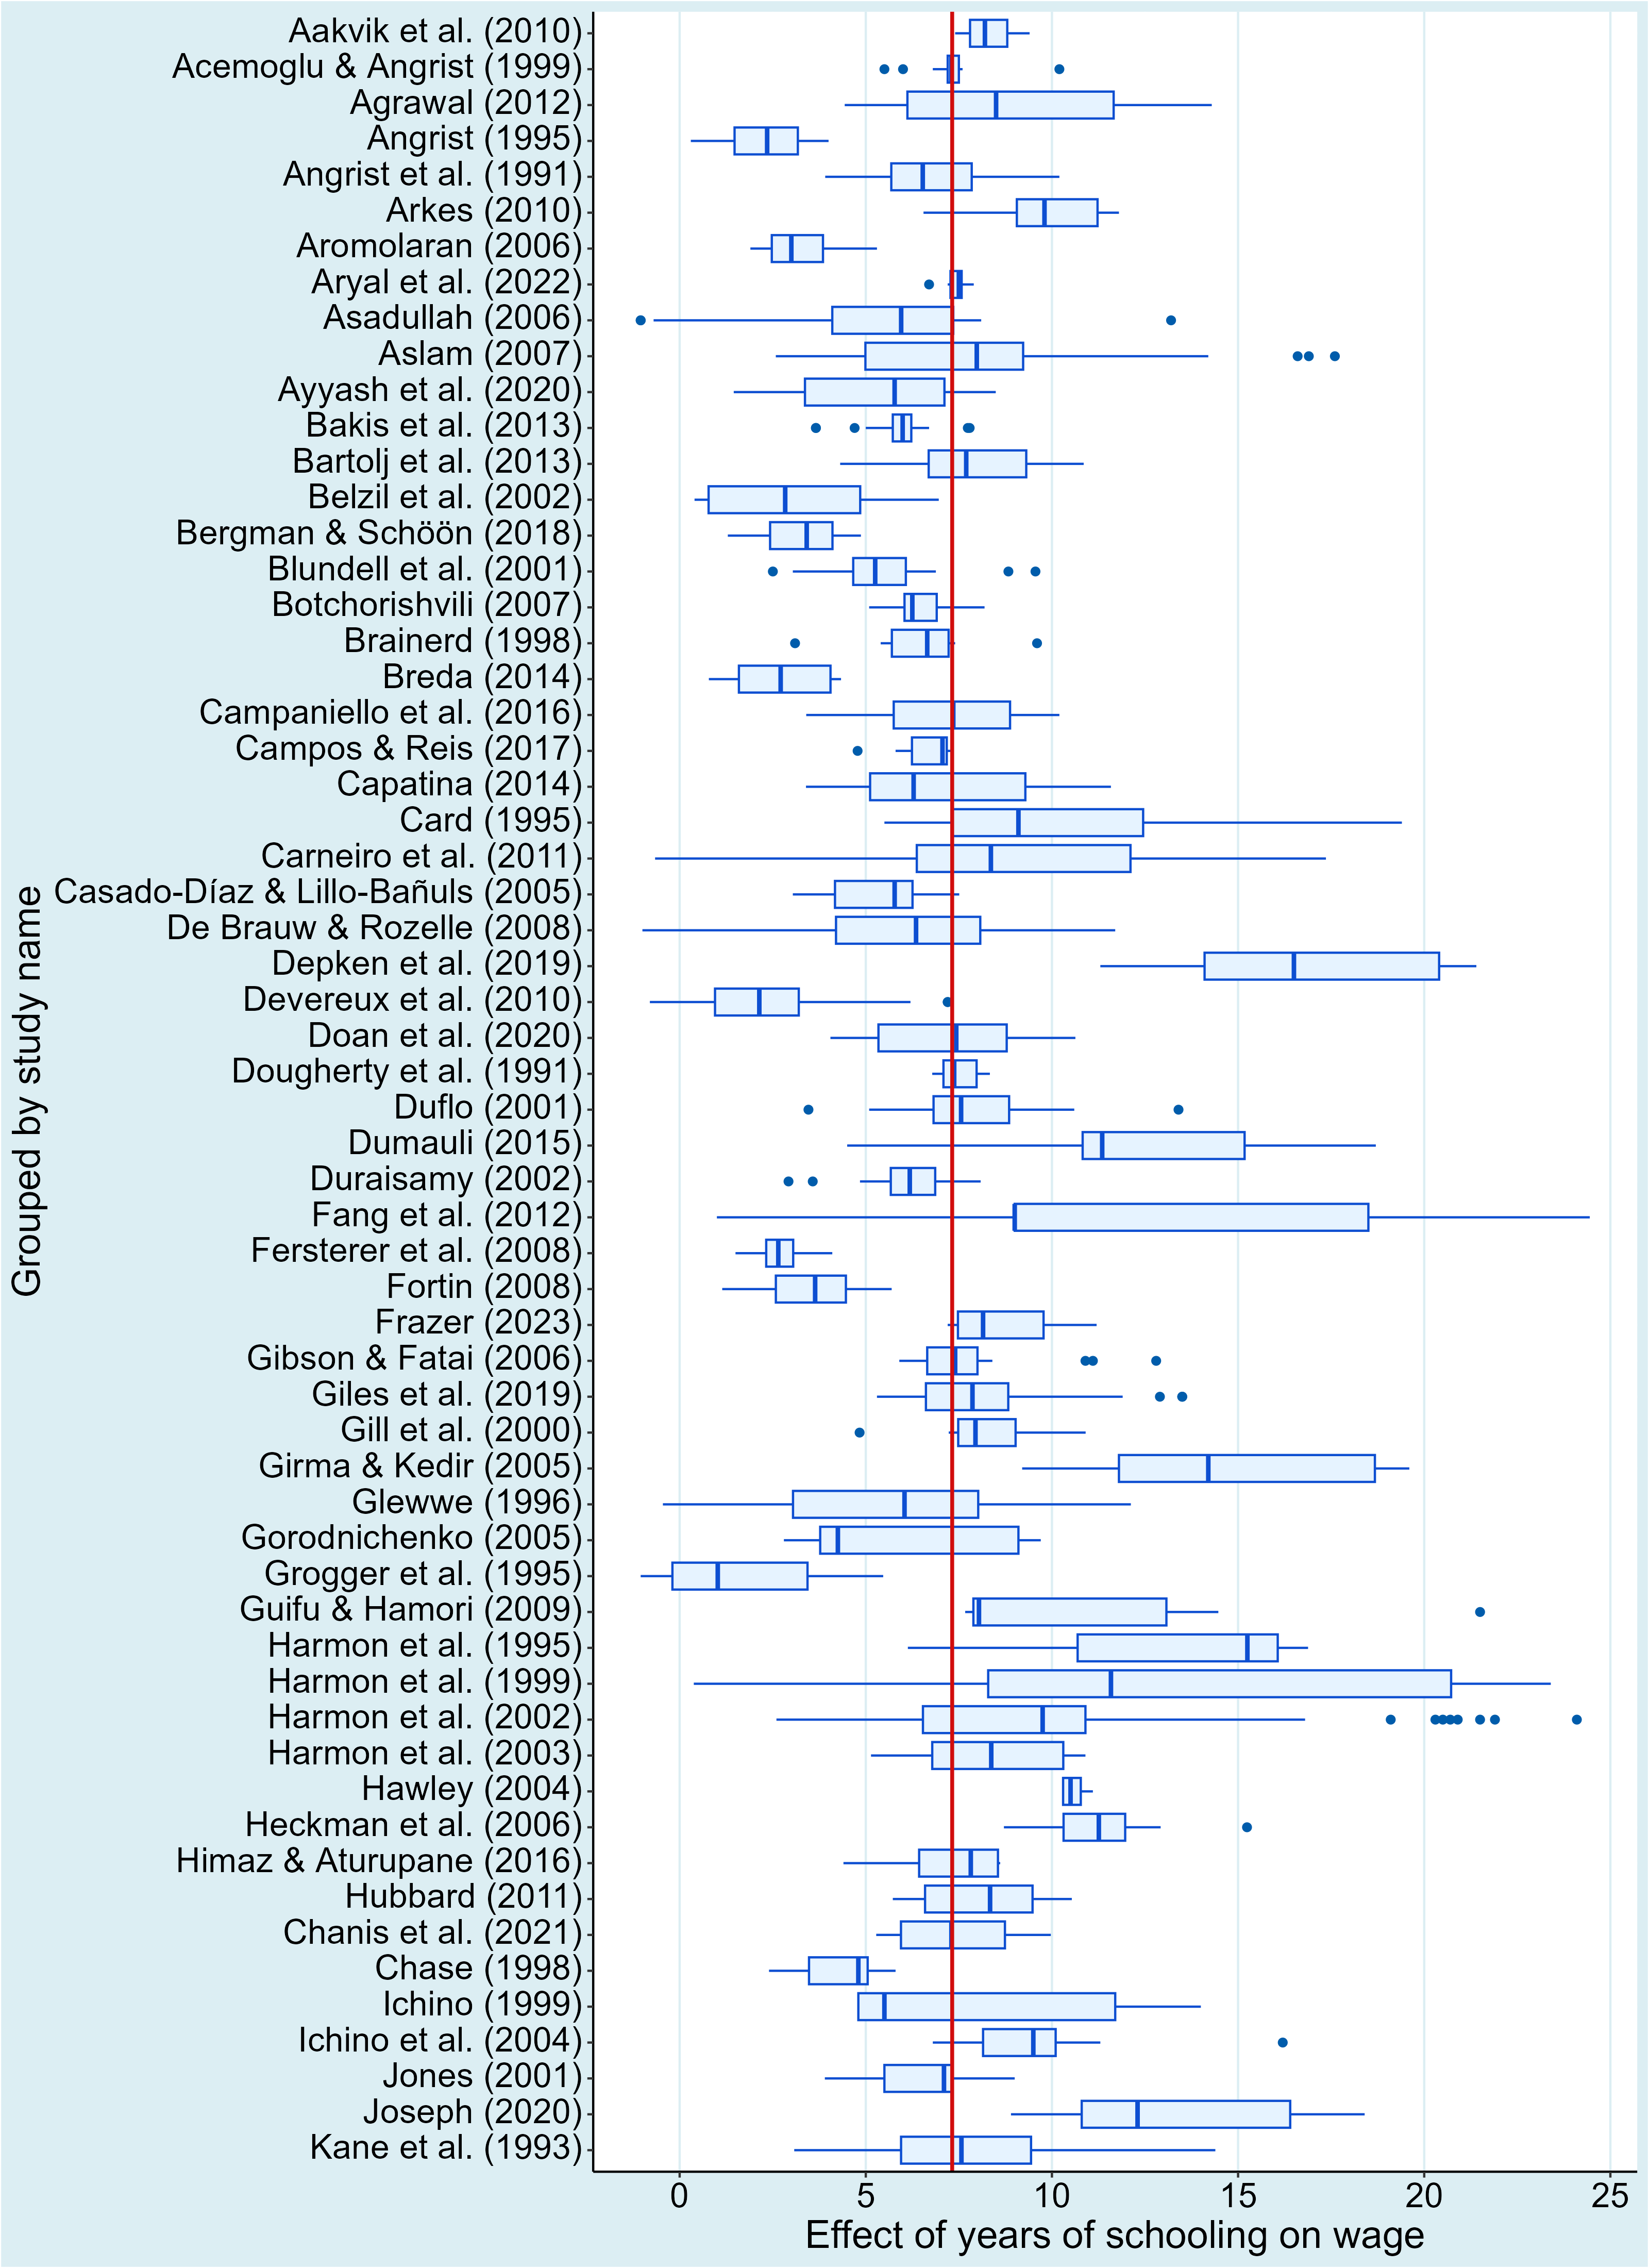
\includegraphics[width=0.9\textwidth]{Figures/box_plot_study_name_1.png}
\end{center}\vspace{-0.7cm}
\captionsetup{width=0.9\textwidth, font = scriptsize}
\caption*{\emph{Note:} This figure shows the first part of a box plot, where the reported estimates are grouped at the study level. The first 60 studies from the dataset are displayed in alphabetically ascending order. The red line represents the average effect across the literature. Each box's length represents the interquartile range between the 25th and 75th percentiles. The dividing line within each box indicates the median value. The whiskers extend to the highest and lowest data points within 1.5 times the range between the upper and lower quartiles. Outliers are depicted as blue dots. The red line depicts the mean of the effect within the data. The data is winsorized at 1\% level.}
\end{figure}
}
\afterpage{
\begin{figure}[!t]
\begin{center}
\caption{Box plot of estimates across individual studies - second part}
\label{fig:box_plot_studies_2}
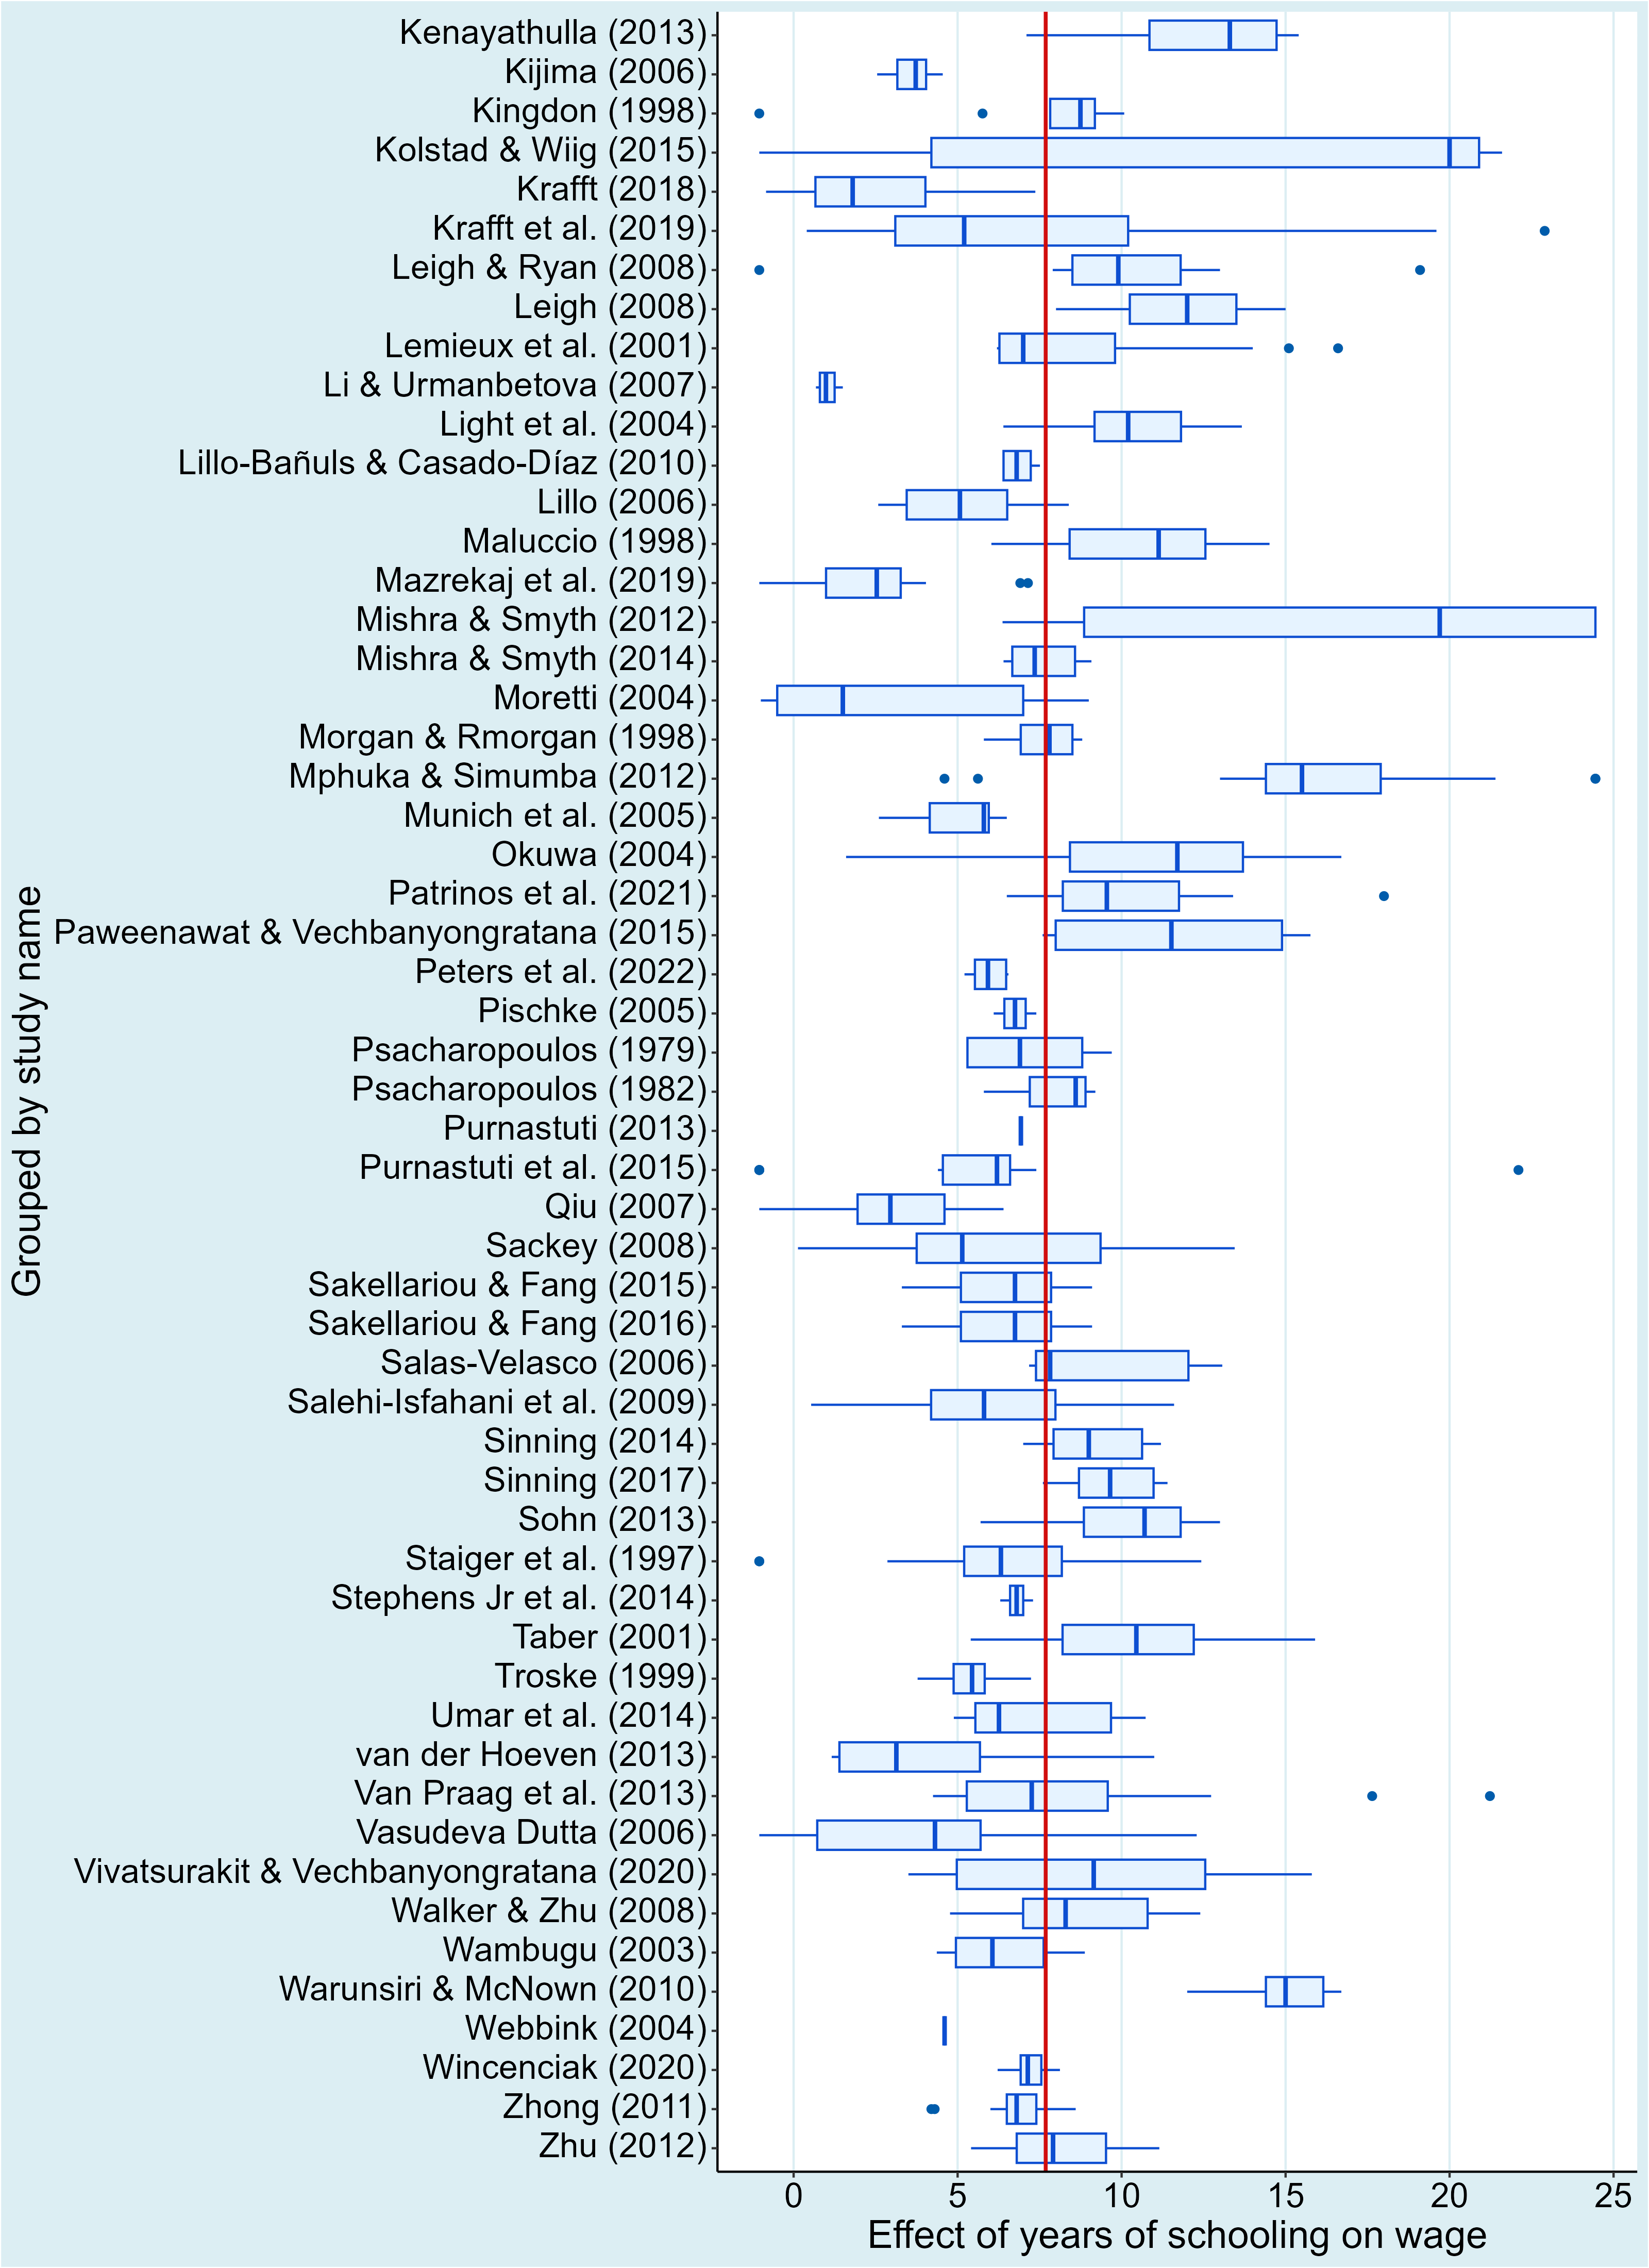
\includegraphics[width=0.9\textwidth]{Figures/box_plot_study_name_2.png}
\end{center}\vspace{-0.7cm}
\captionsetup{width=0.9\textwidth, font = scriptsize}
\caption*{\emph{Note:} This figure shows the second part of a box plot, where the reported estimates are grouped at the study level. Fifty-five remaining studies from the dataset are displayed in alphabetically ascending order. The red line represents the average effect across the literature. Each box's length represents the interquartile range between the 25th and 75th percentiles. The dividing line within each box indicates the median value. The whiskers extend to the highest and lowest data points within 1.5 times the range between the upper and lower quartiles. Outliers are depicted as blue dots. The red line depicts the mean of the effect within the data. The data is winsorized at 1\% level.}
\end{figure}
\clearpage
}

\chapter{Publication bias}
\label{chap:four}
% grammar checked (07-27)

\begin{quoting}
  \textit{An investment in knowledge pays the best interest.}
\end{quoting}
\vspace{-0.2em}
\hfill --- Benjamin Franklin
\vspace{0.5em}

It is widely acknowledged that attending school brings numerous benefits for one's future. To claim the opposite would simply appear foolish, considering the vast quantities of existing literature that explore the positive impact of schooling \citep{oreopoulos2013making, ritchie2018much, heckman2010rate, psacharopoulos2004returns}. However, what happens if a researcher conducts an experiment, and the results suggest that education hurts the prospects of the subjects that took part? Such an experiment will most likely be viewed skeptically, if not frowned upon. The initial response of the publishers presented with such results might, in most cases, go more along the lines of "Perhaps there is something wrong with your setup?" rather than "Heureka, what a discovery!" In expectation of such a response and considering the time and often money invested into the experiment, the researcher is posed with a tough decision - keep the results as is, or sacrifice legitimacy in return for better publication prospects?

The issue described above is commonly referred to as publication bias and is exactly what this part of the paper explores. Among the many forms this malpractice can take, perhaps two are the most prominent. Firstly, studies can remain unpublished due to the discrepancy between their results and the existing knowledge, also known as the \textit{file drawer problem} \citep{stanley2005beyond}. Secondly, the results within those studies may be modified to gain higher order of statistical significance; this can be done by modifying the standard error or even the effect itself - a form of malpractice sometimes referred to as p-hacking \citep{simmons2011false}. Luckily, this manipulation can be detected within the data using various statistical tests, given the unnatural patterns that the p-value distribution tends to exhibit in case such practices are employed.

Regarding publication bias in the literature on returns to education, five of the ten existing meta-analyses address the issue, as mentioned in \autoref{chap:two}. Out of these five studies, three detect the presence of publication bias, while two do not. These conflicting results leave a lot to be desired. For this, I find it crucial to shed more light on the publication bias issue and hope to bring further vital evidence.

In the rest of this chapter, I will first graphically explore the relationship between the effect and the standard effect using a simple visual test. Next, I will conduct multiple linear and non-linear tests to determine whether a quantifiable link exists between the two variables. I will also employ methods that do not assume any prior form of the relationship and test for structural breaks in the distribution of t-statistics in the data. Lastly, I will bring three completely new methods into the picture. These should help me detect p-hacking in the data and link the results together across multiple models with means of model averaging.

\section{Funnel Plot}
\label{sec:funnel_plot}

I first test for publication bias using the funnel plot \citep{Egger1997, stanley2005beyond}. The genius of the method lies in its simplicity, where the main effect is plotted on the x-axis against a measure of precision on the y-axis. Usually (and in this case, too), the precision is calculated simply as the inverse of the standard error. Although \cite{stanley2005beyond} suggests that alternatives can be used, such as the square root of the degrees of freedom, I opt for the standard error. After the plot is constructed, the most precise estimates should be clustered around the true effect mean, assuming that the data contains no publication bias, systematic heterogeneity, or small-sample effects. As precision decreases, the estimates get more scattered, creating an inverted funnel shape. In this shape, gaps or holes hint that data tampering exists within the literature.

As mentioned above, I construct the funnel plot using the inverted standard error as the measure for precision because all estimates in the dataset have their standard error reported (this was one of the conditions during data collection, as described in \autoref{chap:three}). Apart from a funnel plot with all collected data points, I also present a figure that displays only the medians of the effect for all 74 studies. These two graphs appear in the sub-figures of \autoref{fig:funnel_plot}.

\begin{figure}[!t]
  \begin{center}
    \caption{The funnel plot shows no immediately suspicious patterns}
    \label{fig:funnel_plot}
    \begin{subfigure}[b]{0.45\textwidth}
      \caption{All observations}
      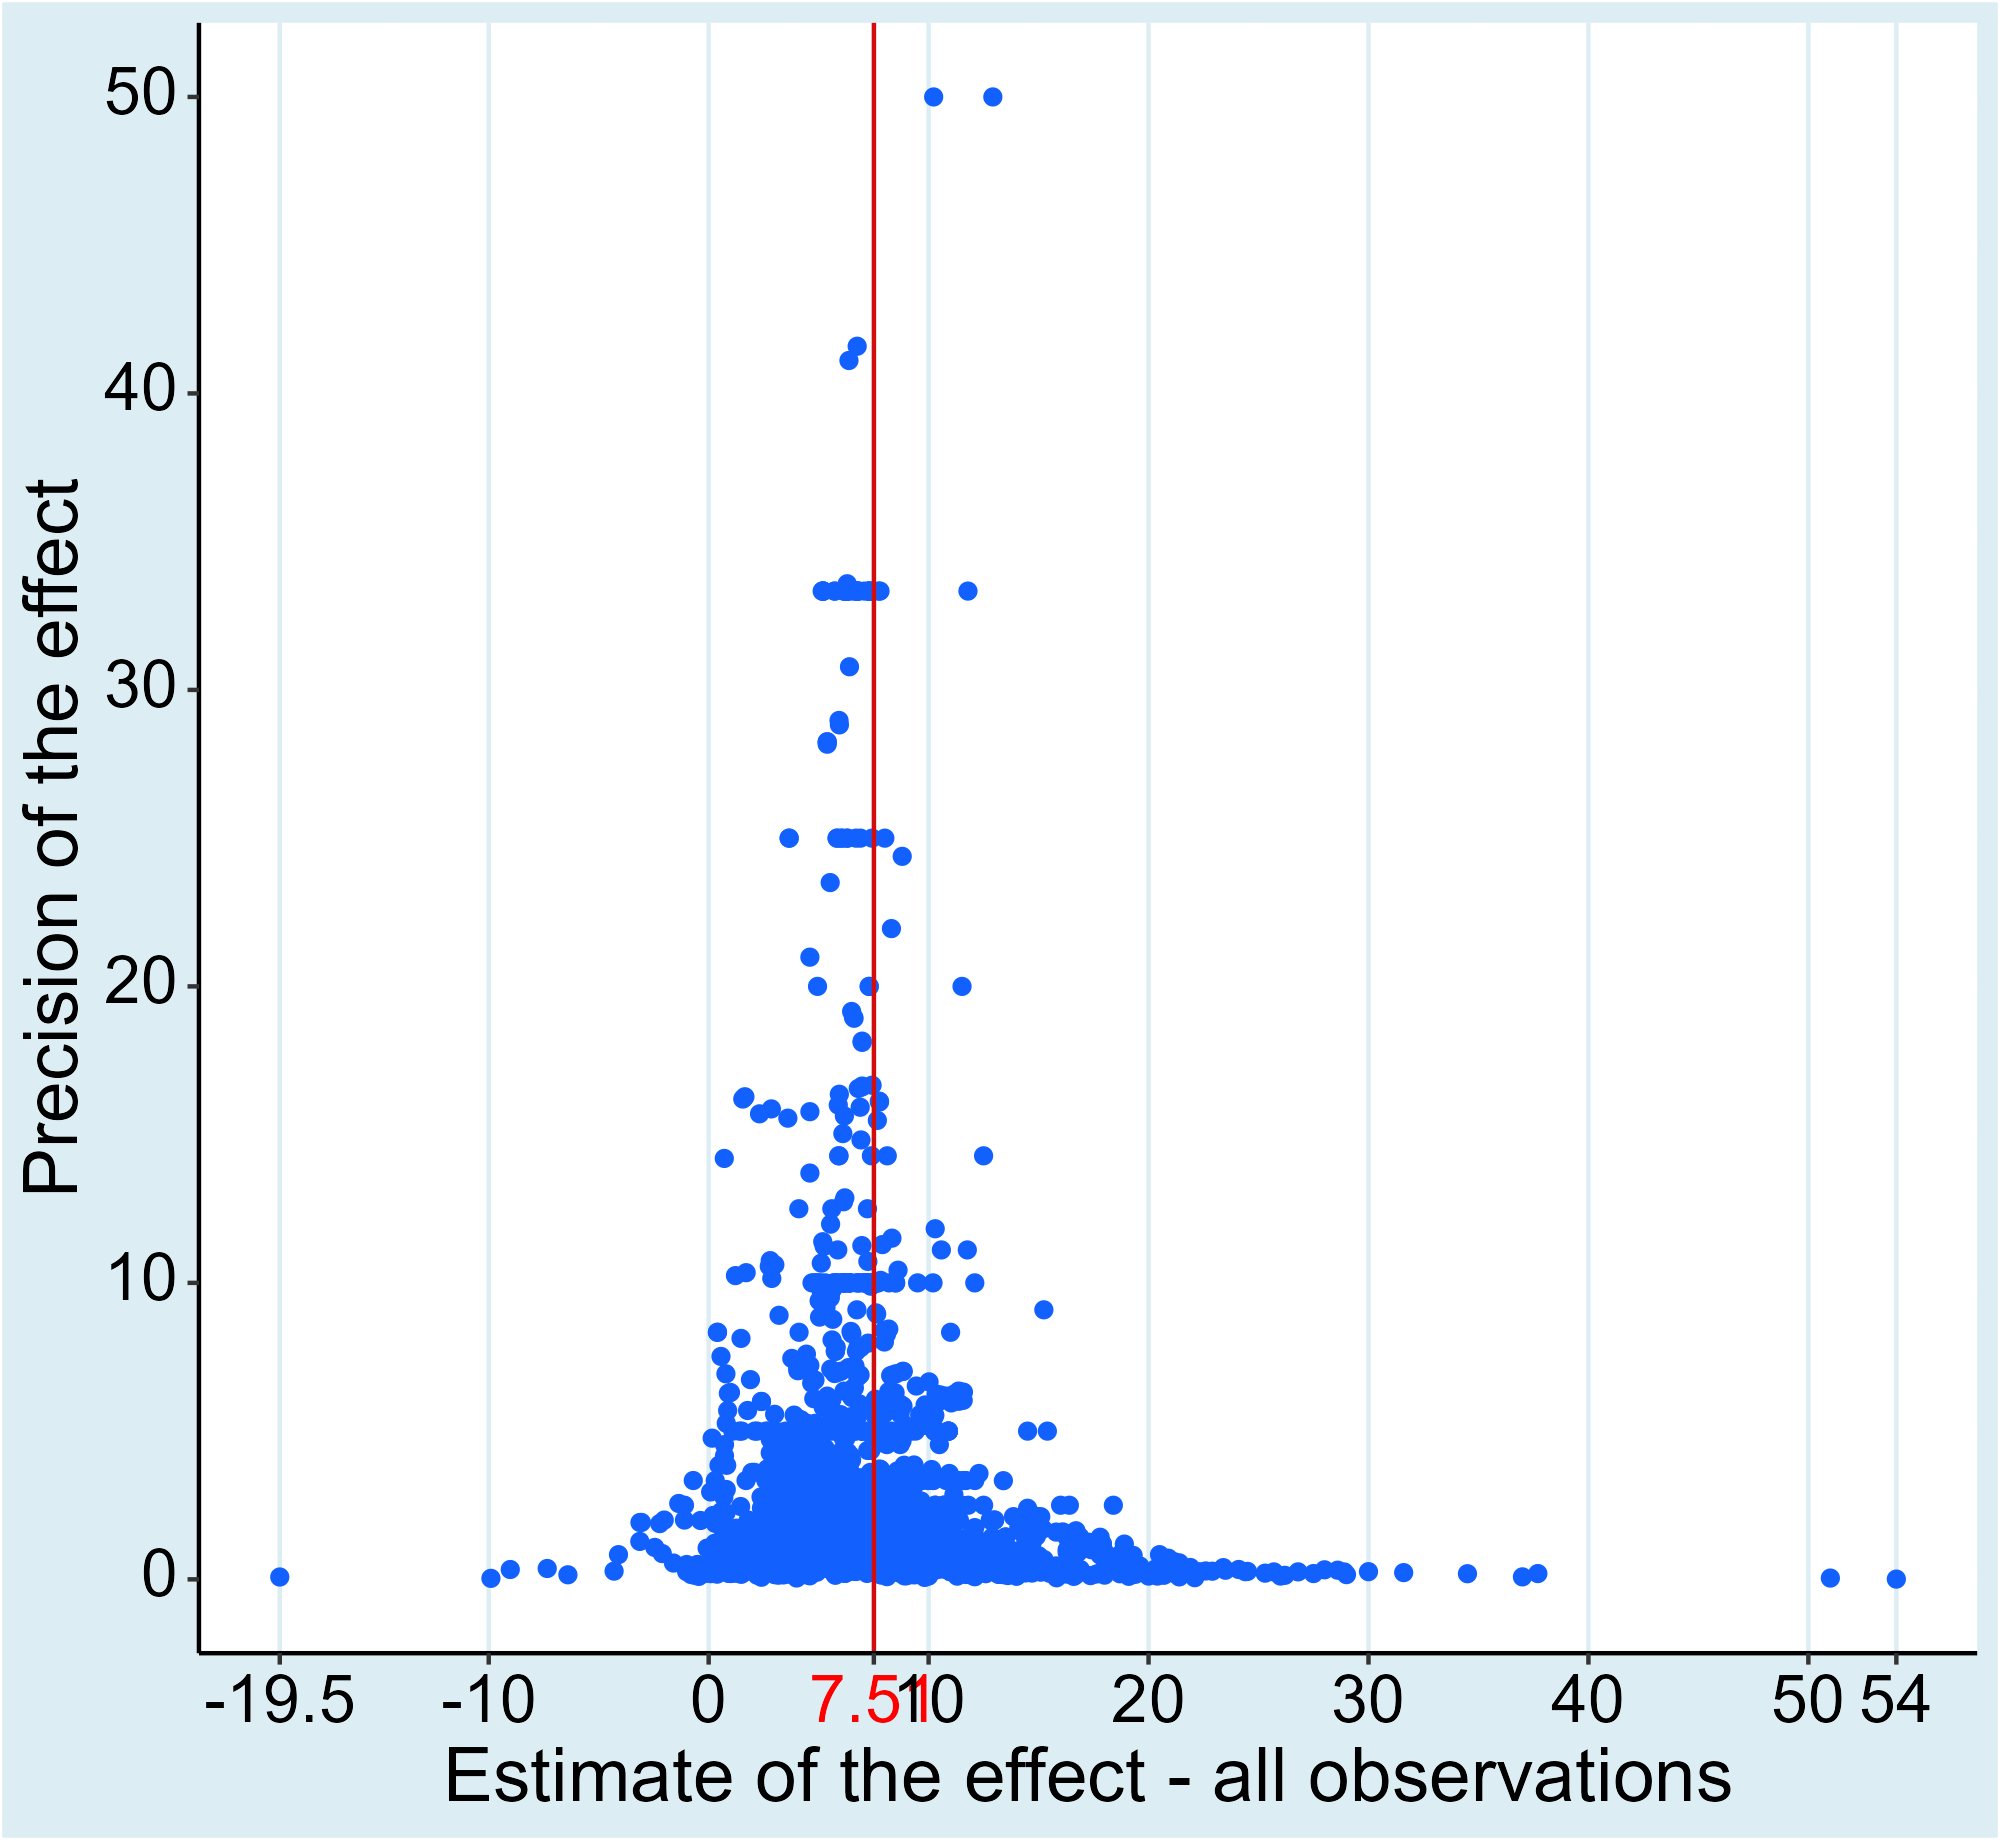
\includegraphics[width=0.95\linewidth]{Figures/funnel.png}
      \label{fig:funnel_plot_all}
    \end{subfigure}
    \begin{subfigure}[b]{0.45\textwidth}
      \caption{Study medians}
      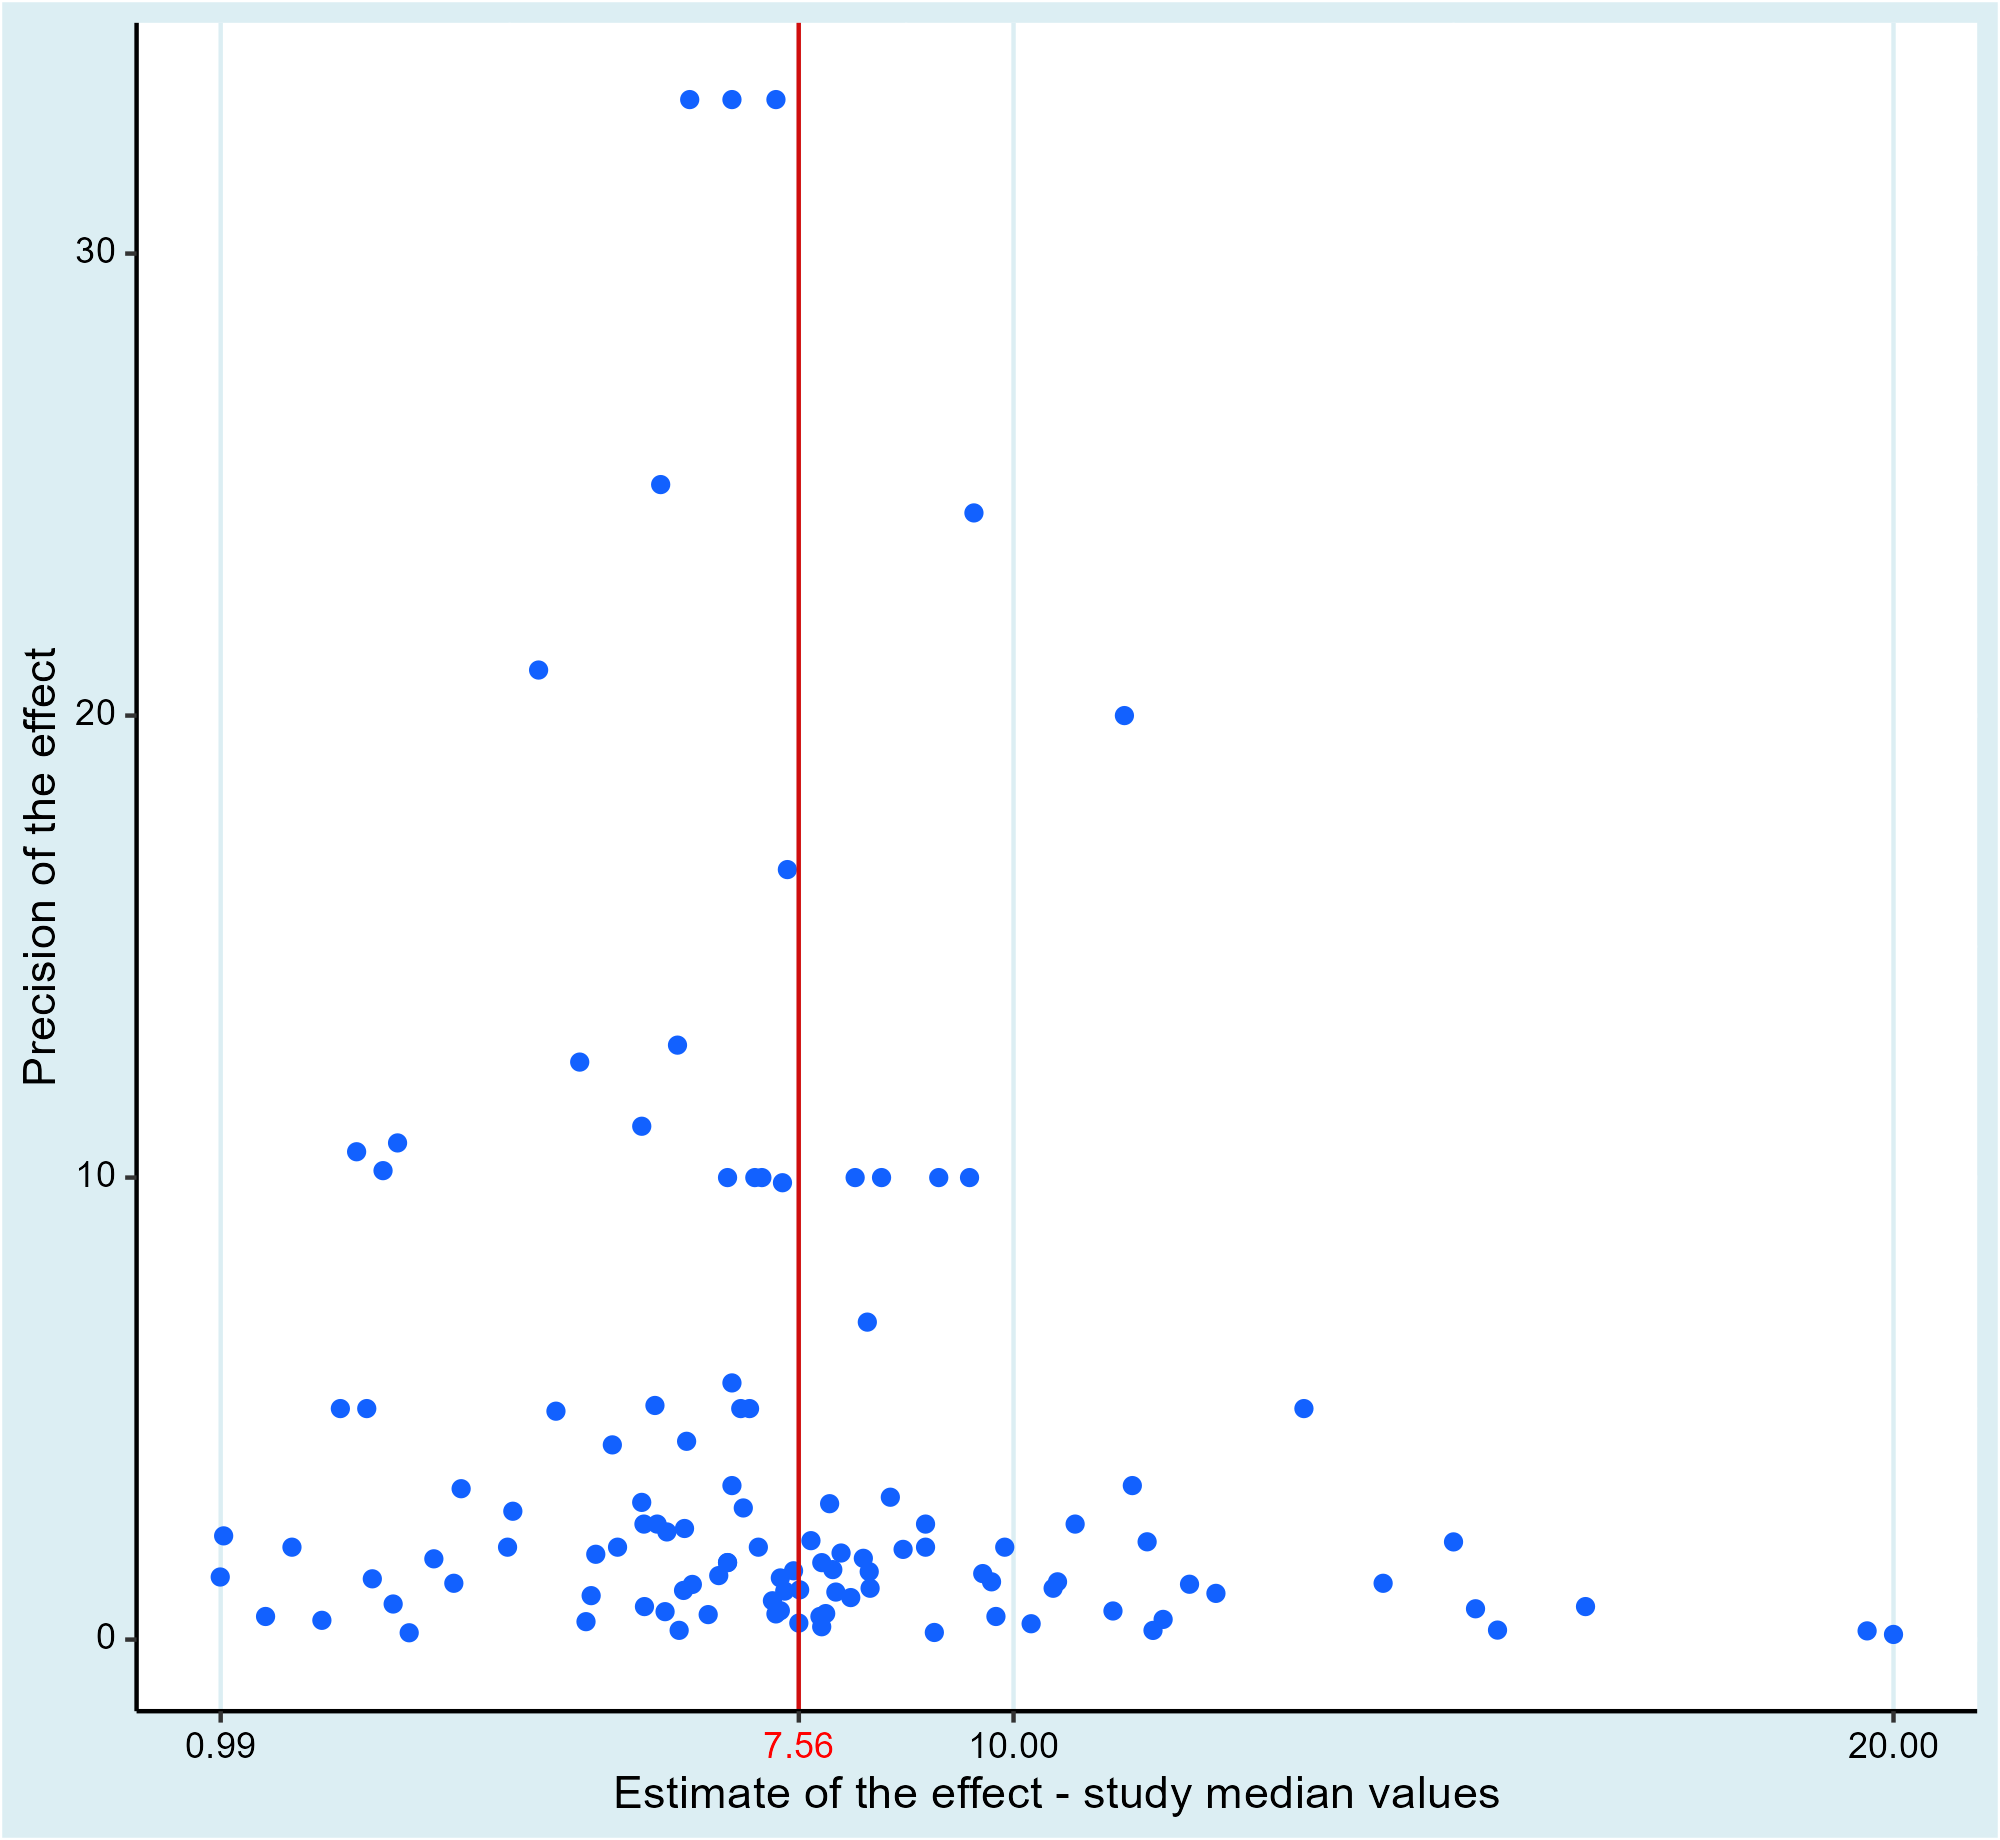
\includegraphics[width=0.95\linewidth]{Figures/funnel_medians.png}
      \label{fig:funnel_plot_medians}
    \end{subfigure}
  \end{center}\vspace{-0.6cm}
  \captionsetup{width=0.85\textwidth, font = scriptsize}
  \caption*{\emph{Note:} This figure displays two funnel plots as per \cite{Egger1997}, where the percentage returns to an additional year of schooling are plotted on the x-axis against precision on the y-axis, measured as $1/SE$ (Standard Error). Plot (a) shows the funnel plot for all observations within the data (1754 data points), while plot (b) shows only the medians of each study (115 data points). The red line marks the mean of these data points. In case of no publication bias, these funnel plots should be symmetrically centered around the true mean.}
\end{figure}

No apparent asymmetry nor holes appear at first glance in the plot with all observations. The less telling plot with study medians exhibits a little more "emptiness" at places, but we can take this simply as a cause of the lower observation count. The crucial takeaway from the latter plot is the lack of suspicious outliers in either direction. Despite this relative consistency, both graphs are perhaps a little more dispersed for higher precision values than the ideal shape might have it. In any case, this is far from enough evidence to claim the presence of publication bias and, contrarily, a hint that the data may be relatively normal.


\section{Funnel Asymmetry Tests}
\label{sec:linear_tests}

% Perhaps refer to the EK paper for theory on FAT-PET-PEESE tests

The funnel plot itself, albeit a quick and easy way of detecting obvious publication bias, is still a less precise method that relies on \textit{eye-balling} and subjective interpretation, both hardly rigorous ways of conducting research. To establish the results quantitatively and more robustly, I turn first to the \ac{FAT-PET} \citep{Egger1997, stanley2005beyond, stanley2008fatpet}.

These techniques test for the funnel plot asymmetry using a simple equation that regresses the effect on its standard error to uncover any correlation between the two. If such a correlation exists, it can be interpreted as a systematic relationship between the effect and its standard error, indicating publication bias. Algebraically, the relationship can be written as:

\begin{equation}\label{eq:fat_reg}
  S_{ij} = \beta_0 + \beta_1 * (SE_{S})_{ij} + u_{ij},
  \vspace{0.3cm}
\end{equation}

where $S$ represents the returns to schooling effect for the i-th observation of the j-th study in the dataset, and $SE_{S}$ corresponds to the effect's standard error. The slope coefficient, $\beta_1$, then measures the publication bias in the data, while the intercept coefficient, $\beta_0$, captures the "true" effect of returns to schooling corrected for publication bias. $u_{ij}$ stands for the error regression term. In the tables below, I will refer to the slope coefficient with the label \textit{Publication bias}, while the intercept will be labeled as \textit{Effect beyond bias}.

If no publication bias is present in the data, the slope coefficient will be either 0 or close to it. Conversely, higher absolute values would indicate the opposite correlation between the effect and its standard error, thereby suggesting publication bias is present in the data. This is motivated by the assumption that both the effect and its standard error should be, statistically speaking, drawn from an independent, statistically symmetrical distribution. However, practically speaking, this is rarely the case.

The results of the funnel asymmetry tests can be viewed in \autoref{tab:PB-FAT}. Firstly, I include a simple \ac{OLS} model, followed by two models accounting for unobserved heterogeneity in the form of Fixed effect and Random effect estimators. Lastly, I introduce two models that weigh the equation, first by the inverse of the number of observations reported per study and second by precision. The motivation behind the last two models is to account for unobserved heterogeneity and heteroskedasticity, respectively. For robustness, I cluster all standard errors at the study level, and append wild bootstrap confidence intervals where possible. These I calculate using an iteration sample of 100 for each method.

Looking at concrete results, four out of five of these methods find a statistically significant presence of publication bias, and all claim the underlying effect lies within the range of 6 and 7 percent. This indicates that the underlying effect might be slightly lower than the simple estimates' average, approximately by one percentage point. Furthermore, the lowest predicted value can be associated with the study-size weighted model ($\sim$6.3), suggesting perhaps that studies of larger size drive the effect upwards. However, it is essential to note that this difference is relatively small compared to the other estimates. The discrepancy between the study-size weighted model and the fixed-effects model, the latter of which predicts the highest rate of returns to education at 6.7 percent, is less than half a percentage point. All of these results also pose a rather high level of statistical significance, save for the precision-weighted model. Apart from this model, too, the wild confidence intervals align with the study-level clustered ones. The precision-weighted model's publication bias coefficient casts a shadow of suspicion on the influence of highly precise studies. Given the wide confidence interval, it appears unfeasible to claim that an unexpected effect is at place, but rather that there is a lack thereof. Perhaps further tests may help shed more light on the issue.

% Linear tests
\begin{table}[!t]
  \centering
  \footnotesize
  \singlespace
  \caption{Linear tests for publication bias}
  \label{tab:PB-FAT}
  \begin{tabular}{
      @{\hskip\tabcolsep\extracolsep}
      l*{3}{c}} %one left column, three center (*{} makes the cols inherit attributes)
    \toprule
    \multicolumn{1}{l}{}               &
    \multicolumn{1}{c}{\textbf{OLS}}   &
    \multicolumn{1}{c}{\textbf{Study}} &
    \multicolumn{1}{c}{\textbf{Precision}}                                                \\
    \midrule

    Publication Bias                   & 0.832**        & 1.169***      & 0.262           \\
    \emph{\hspace{0.2cm}SE}            & (0.097)        & (0.121)       & (0.425)         \\
    \emph{\hspace{0.2cm}Bootstrap CI}  & [0.624, 1.035] & [0.92, 1.405] & [-0.833, 1.091] \\
    \addlinespace[0.5em]
    Effect Beyond Bias                 & 6.408***       & 6.294***      & 6.54***         \\
    \emph{\hspace{0.2cm}SE}            & (0.118)        & (0.153)       & (0.168)         \\
    \emph{\hspace{0.2cm}Bootstrap CI}  & [6.164, 6.639] & [6.04, 6.645] & [6.189, 6.918]  \\
    \addlinespace[0.5em]
    Total observations                 & 1,754          & 1,754         & 1,754           \\

    \midrule
    \multicolumn{1}{l}{}               &
    \multicolumn{1}{c}{\textbf{FE}}    &
    \multicolumn{1}{c}{\textbf{BE}}    &
    \multicolumn{1}{c}{\textbf{RE}}                                                       \\
    \midrule

    Publication Bias                   & 0.746***       & 0.752***      & 0.747***        \\
    \emph{\hspace{0.2cm}SE}            & (0.06)         & (0.244)       & (0.058)         \\
    \emph{\hspace{0.2cm}Bootstrap CI}  &                &               & [0.514, 0.995]  \\
    \addlinespace[0.5em]
    Effect Beyond Bias                 & 6.517***       & 6.741***      & 6.708***        \\
    \emph{\hspace{0.2cm}SE}            & (0.107)        & (0.418)       & (0.294)         \\
    \emph{\hspace{0.2cm}Bootstrap CI}  &                &               & [6.398, 6.965]  \\
    \addlinespace[0.5em]
    Total observations                 & 1,754          & 1,754         & 1,754           \\

    \bottomrule
    \multicolumn{4}{>{\scriptsize}p{0.85\linewidth}}{\emph{Note:} The table displays the results obtained from estimating \autoref{eq:fat_reg} SE = Standard Error, CI = Confidence Interval, OLS = Ordinary Least Squares. FE = Fixed Effects. BE = Between Effects. RE = Random Effects. Precision = Estimates are weighted by the inverse standard error. Study = Estimates are weighted by the inverse number of observations reported per study. Standard errors, clustered at the study level, are included in parentheses. Wild bootstrap confidence intervals at 95\% confidence level, bootstrapped over 100 iterations, are reported in brackets. ***p<0.01, **p<0.05, *p<0.1}
  \end{tabular}
\end{table}



\section{Non-linear Tests}
\label{sec:nonlinear_tests}

The relationship between the effect and its standard error, as described in \autoref{eq:fat_reg}, is assumed to be linear in the funnel asymmetry tests. However, it is crucial to acknowledge that this assumption does not always hold. In cases where the relationship behaves less straightforwardly, the \ac{FAT-PET} tend to underestimate the underlying effect if it differs from zero \citep{stanley2014meta}. In the context of my data, this concern may be valid since most of the data points are positive and occasionally even reach double digits. To address potential non-linear forms of the relationship that may appear in the data, I present six techniques that relax the linearity assumption.

The first is the \ac{WAAP}, introduced by \cite{Ioannidis2017Waap}. Their proposition involves the application of unrestricted \ac{WLS} only on observations of adequately powered studies. "Power" here refers to a study's ability to detect whether an effect if it is truly present in the data. The more power a study has, the bigger its reliability. In technical terms, the power is calculated using the statistical significance of estimates and then compared to their standard errors. As per the original paper, I kept only the estimates of studies that display power over 80\%. Strikingly, 1469 out of the 1754 estimates in my dataset get identified as adequately powered. Using these estimates, \ac{WAAP} then proposes an estimate of 6.9\% which is slightly higher than any of the linear models presented in \autoref{tab:PB-FAT}.

The second approach, proposed by \cite{Stanley2010Top}, entails discarding 90\% of data and keeping only the top 10 percent with the highest precision. This somewhat paradoxical approach stems from the idea that most researchers use statistical significance as the primary benchmark for deciding whether to publish the estimate. \cite{Stanley2010Top} show that if most of the less precise estimates are discarded, the publication bias within the data sample drops considerably. In my data, 10\% of estimates correspond to 176 observations. The Top10 model yields a modest result of 6.4\%.

\cite{Furukawa2019Stem} chooses a similar tactic by selecting a specific number of the most precise estimates. The cutoff is determined by minimizing mean square error; this aims at striking a balance between variance/efficiency and bias. The selected points from what is referred to as "stem" are those with the lowest mean square error. The author suggests using a \textit{representative sample} for the calculation, rather than a full data sample. Arbitrarily, I chose study medians to generate this subsample, which yielded a total of 115 data points. You may find a visual representation of this method in \autoref{fig:stem}. The rate of returns to education suggested by this approach is at around 6.7\%, very much in line with the other regression-based results obtained thus far.

\sidecaptionvpos{figure}{t}
\begin{SCfigure}
  \centering
  \captionsetup{font = scriptsize}
  \caption[Stem-based method]{\vspace{0.5cm}Stem-based method\\ \emph{Note:} This figure displays a non-linear estimation of the true effect \citep{Furukawa2019Stem}. The main effect, labeled \textit{Coefficient $\beta$}, is plotted on the x-axis against precision, calculated as $log(SE)$ (Standard Error). The yellow diamond and the whiskers of the same color denote the 95\% confidence interval of the stem-based estimate of the effect. The dark grey line indicates the predicted estimates throughout various levels of data, while the purple diamond shows the minimal precision value above which lies the stem. The blue circles then represent the individual effect estimates. Median of each study was the measure chosen as the representative sample of observations for the input data, resulting in 115 total data points.}
  \label{fig:stem}
  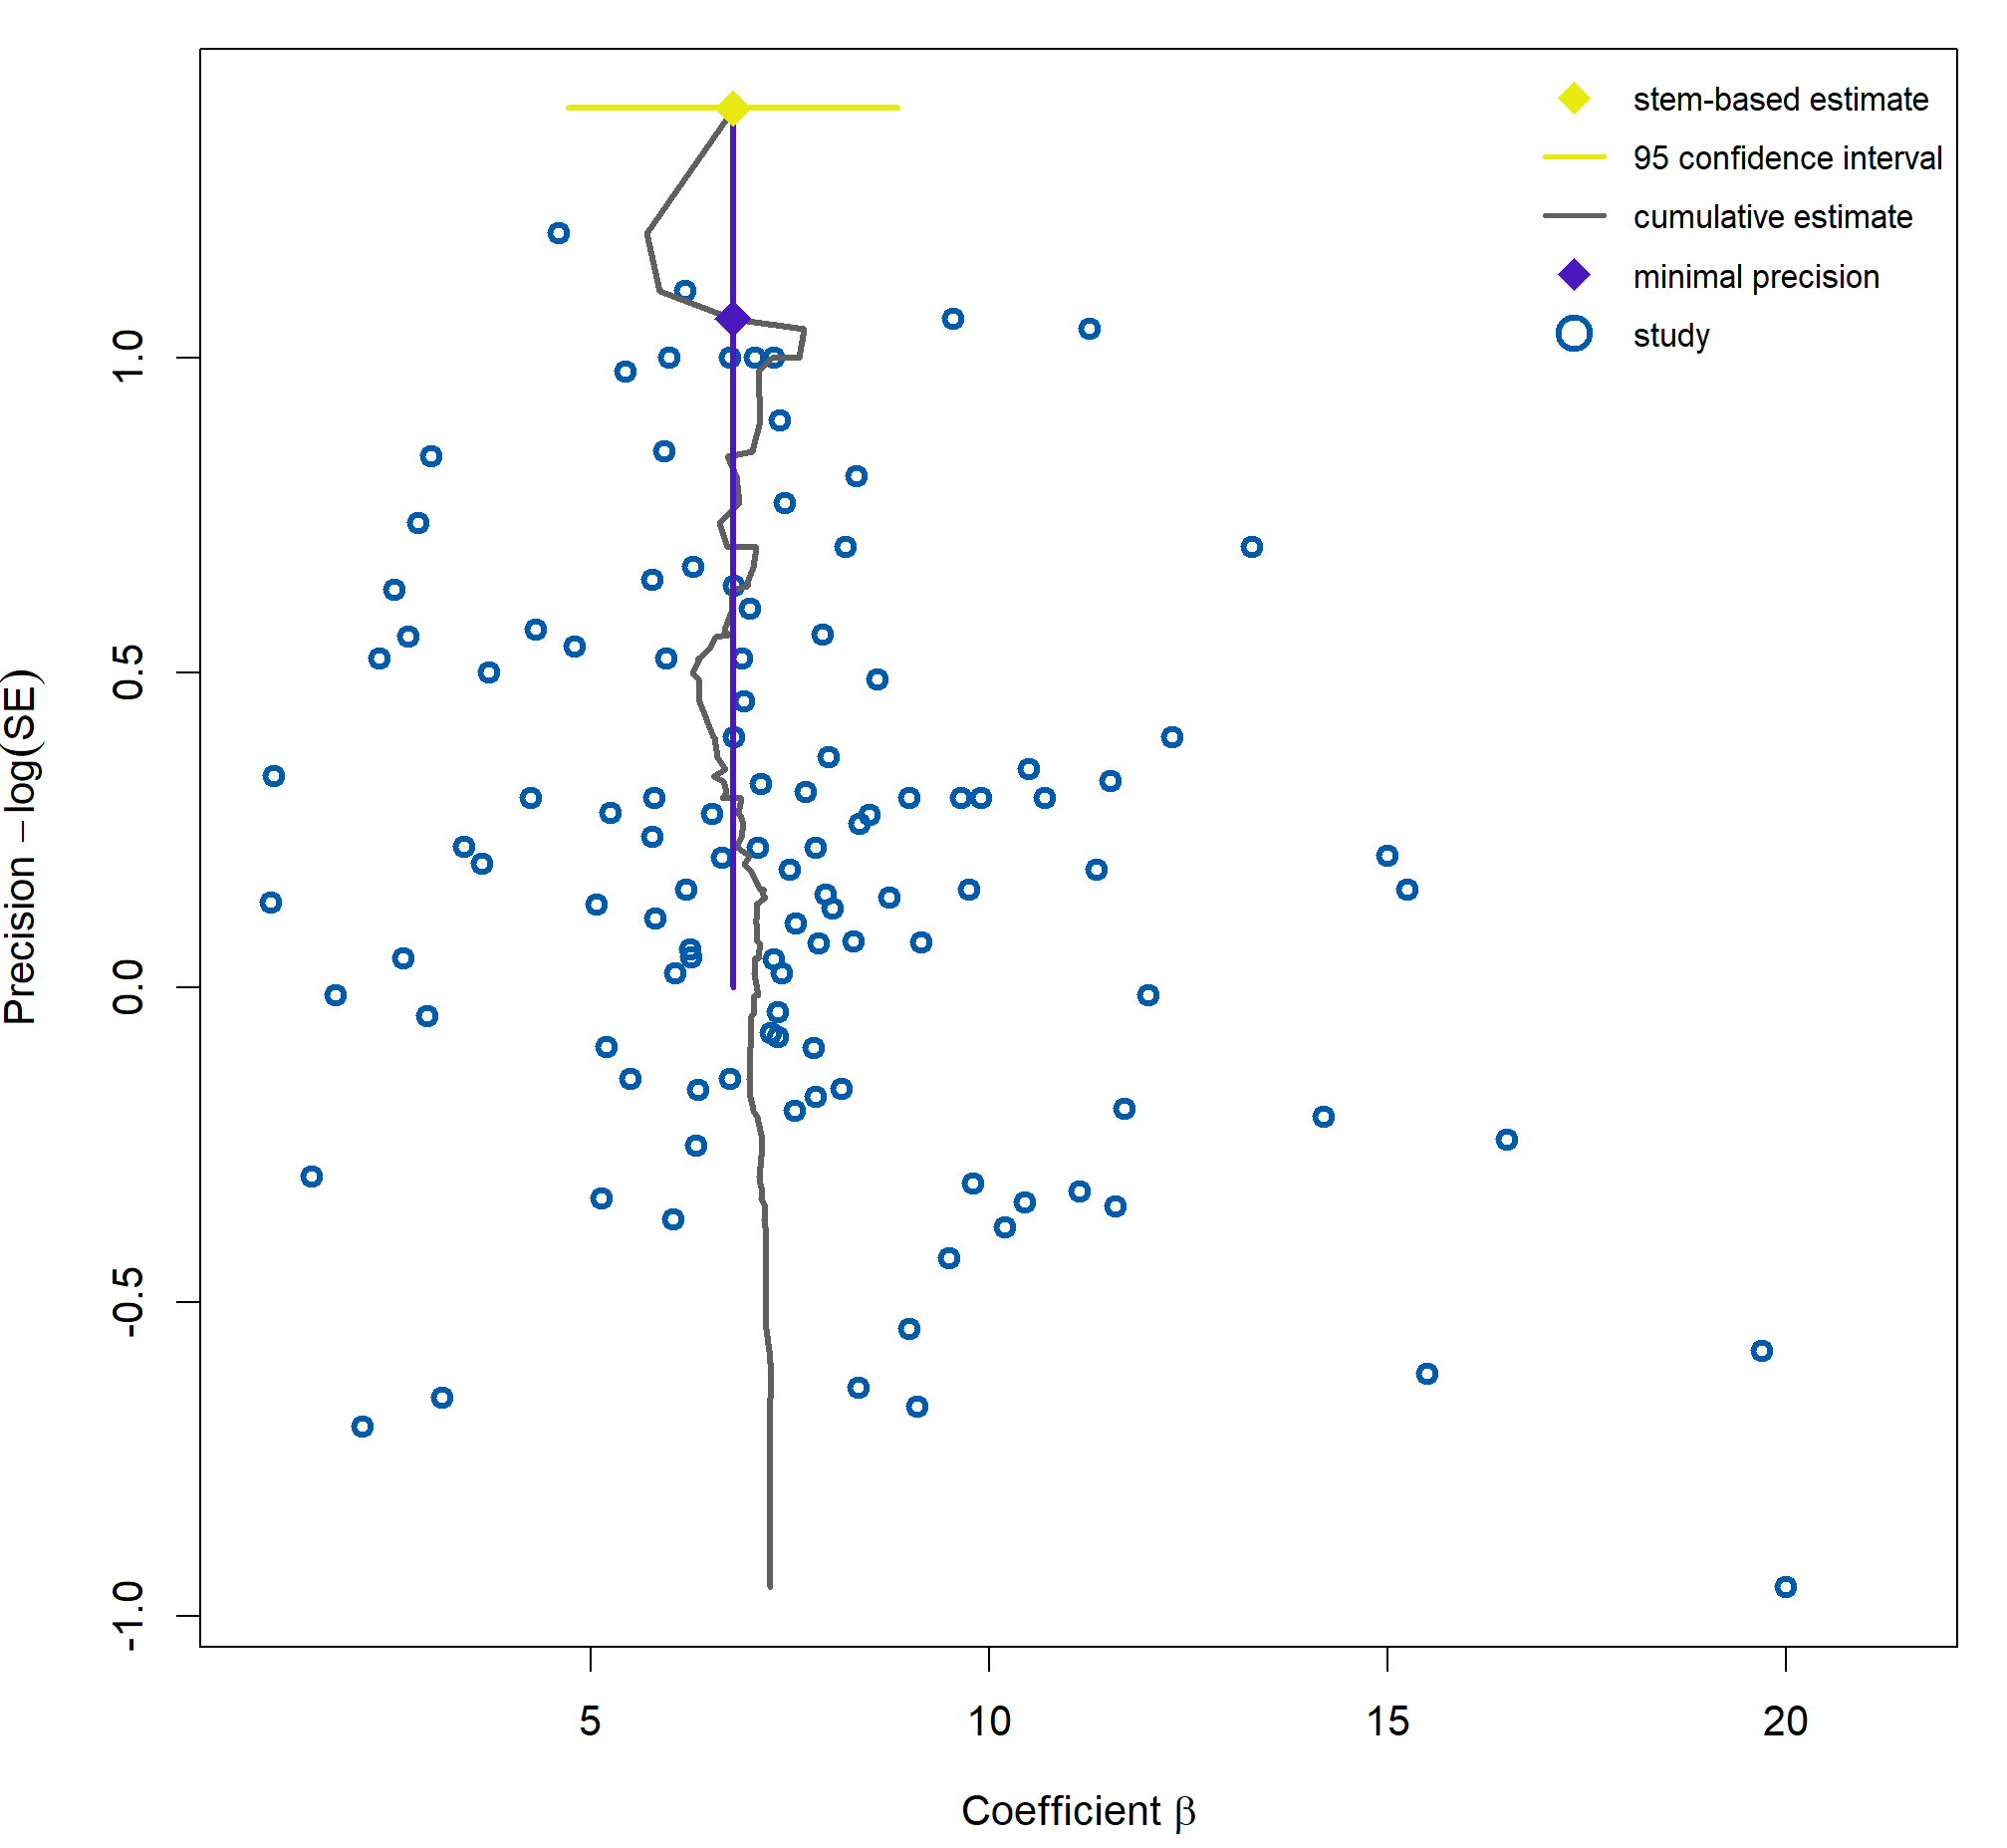
\includegraphics[width=0.5\textwidth]{Figures/stem.png}
\end{SCfigure}

Further, I estimate the Hierarchical Bayes model by \cite{Allenby2006Hier}. The procedure employs Bayesian statistics to leverage variability within individual studies to determine the weights of individual observations aggregated at the study level. The model parameters get treated as random variables instead of fixed numbers, allowing for variability at multiple levels within the dataset. As such, different units can have comparable sharing strength, allowing for more robust estimates. The hierarchical part stems from the fact that priors are specified using another model (called hyperprior) instead of a direct specification, as is usually done in Bayesian modeling. This complex multi-level modeling framework yields an estimate of 6.8\% in my case. Additionally, the analysis suggests the presence of publication bias at a significance level of 1\%.

% Non-linear tests
\begin{table}[!b]
  \centering
  \footnotesize
  \singlespace
  \caption{Nonlinear tests for publication bias}
  \label{tab:N-L}
  \begin{tabular}{
      @{\hskip\tabcolsep\extracolsep}
      l
      *{6}{c}
      @{}
    } %0.15 0.65
    \toprule
    \addlinespace[0.5em]
    \multicolumn{1}{c}{}               &
    \multicolumn{1}{c}{\textbf{WAAP}}  &
    \multicolumn{1}{c}{\textbf{Top10}} &
    \multicolumn{1}{c}{\textbf{Stem}}  &
    \multicolumn{1}{c}{\textbf{Hier}}  &
    \multicolumn{1}{c}{\textbf{AK}}    &
    \multicolumn{1}{c}{\textbf{Kink}}                                                                  \\
    \midrule
    Publication Bias                   &         &          &          & 0.504*** & 2.764*** & 0.262   \\
    \emph{\hspace{0.2cm}SE}            &         &          &          & (0.165)  & (0.112)  & (0.39)  \\
    \addlinespace[0.5em]
    Effect Beyond Bias                 & 6.9***  & 6.439*** & 6.783*** & 6.801*** & 6.548*** & 6.54*** \\
    \emph{\hspace{0.2cm}SE}            & (0.092) & (0.146)  & (1.055)  & (0.269)  & (0.091)  & (0.054) \\
    \addlinespace[0.5em]
    Total Observations                 & 1,754   & 1,754    & 115      & 1,754    & 1,754    & 1,754   \\
    \addlinespace[0.5em]
    Model observations                 & 1,469   & 176      &          &          &          &         \\
    \bottomrule
    \multicolumn{7}{>{\scriptsize}p{0.95\linewidth}}{\emph{Note:} The table reports estimates of the effect beyond bias using six non-linear methods and estimates of the publication bias obtained using two of these methods. WAAP = Weighted Average of the Adequately Powered \citep{Ioannidis2017Waap}. Top10 = Top10 method by \cite{Stanley2010Top}. Stem = the stem-based method by \cite{Furukawa2019Stem} where P represents the probability of results insignificant at 5\% being published relative to the probability of the significant ones at the same level. Hier = Hierarchical Bayes model \citep{Allenby2006Hier}. AK = \cite{Andrews2019Selection}'s Selection model. Kink = Endogenous kink model by \cite{Bom2019Kink}. SE = Standard Error. Standard errors, clustered at the study level, are included in parentheses. ***p<0.01, **p<0.05, *p<0.1 }
  \end{tabular}
\end{table}


The next test is the Selection model proposed by \cite{Andrews2019Selection}. The authors argue that the publication probability for estimates remains constant at similar levels of statistical significance, a concept called "conditional publication probability." Once a certain statistical significance threshold is crossed, the publication probability changes. \cite{Andrews2019Selection} then demonstrate how this probability can be calculated non-parametrically, and utilizing the inverse of this probability as new weights, they obtain a non-biased distribution of the estimates. Using a t-distribution at the 5\% significance level (cutoffs for $p(.)$ set to 1.96), I obtain the result of around 6.5\%. The method also proposes that estimates at the 5\% significance level are more likely to be published than insignificant ones (P = 2.7).

As the last of the non-linear techniques testing for publication bias, I add the \ac{EK} model introduced by \cite{Bom2019Kink}. Using the argument that the publication bias is usually absent for sufficiently large studies, the \ac{EK} model finds a cutoff value below which publication bias should not appear. \cite{Bom2019Kink} then fit a piecewise linear regression with a kink at this cutoff point, allowing non-linearity in the model. An advantage of this approach is that this method reduces to a simple linear model as the effect approaches zero, where said linear methods perform well. As such, the \ac{EK} approach should provide more robust results than its linear counterpart. In my case, the suggested value of the main effect is 6.54\%, which falls right into the average of the rest of the (both linear and non-linear) results. The model also provides a non-significant estimate of the presence of publication bias. This marks the last of non-linear methods; all of the results obtained from these estimations can be found in \autoref{tab:N-L}.

Every single one of the six models propose a statistically significant effect beyond bias within the 6 to 7 percent range. These results align with the linear approach and confirm the behavior observed thus far. The Hierarchical Bayes indicates a strong presence of publication bias, while the Endogenous Kink method result is insignificant. Finally, the Selection model proposes that results at the 5\% significance level have a considerably higher chance of publication than insignificant ones.


\section{Tests Without the Exogeneity Assumption}
\label{sec:exo_tests}

Until now, the publication bias tests have been based on the assumption that the correlation between the effect and the standard error indicates publication bias. However, this introduces, by definition, endogeneity into the equation. To see how this issue can be treated, it is essential to understand how it arises in the first place.

The correlation in the data, and thus endogeneity, can come from several sources. First, it could be a simple measurement error or wrong calculation procedure that introduces correlation into the data; the standard error, too, is an estimate, after all. Second - this is what the publication bias gets associated with perhaps the most - the endogeneity may arise from a conscious and deliberate tampering of the standard error to improve significance. And lastly, any unobserved heterogeneity may also introduce correlation, this time in the form of inherent methodological differences that may systematically influence the results. To display the estimate-error relationship clean of endogeneity, I utilize two techniques - \ac{IV} regression and p-uniform* \citep{vanAert2021puni}.

First, the \ac{IV} regression, for which we need an instrument. The criteria for finding a valid one are relatively simple - it should be a metric that somehow captures the behavior of (correlates with) standard error while having no relationship to the estimate. Using such metric, it should be possible to derive the publication bias coefficient ($\beta_1$ from \autoref{eq:fat_reg}) not poisoned by endogeneity. Several instruments appear valid here, including $\frac{1}{\sqrt{n_{\text{obs}}}}$, $\frac{1}{n_{\text{obs}}}$, $\frac{1}{n_{\text{obs}}^2}$, and $\log(n_{\text{obs}})$, where $n_{\text{obs}}$ stands for the number of observations associated with each estimate. The number of observations variable holds several inherent properties that make all these instruments valid options. Firstly, the size of an experiment, or the number of subjects in the study, does not directly change the population-wide effect. If such a true effect exists, it should be independent of how many subjects we include in the analysis. Secondly, the standard error decreases as the sample size increases. This is a fundamental principle of statistics. In other words, the more subjects there are in the study, the bigger the confidence that the findings based on that sample are close to the results had the whole population been used for calculation.

%Table with the results of the IV/p-uni* tests
\begin{table}[!t]
  \centering
  \footnotesize
  \singlespace
  \caption{Relaxing the exogeneity assumption}
  \label{tab:IV-p}
  \begin{tabular}{
      @{\hskip\tabcolsep\extracolsep}
      l
      *{2}{c}
      @{}
    }
    \toprule
    \multicolumn{1}{l}{}                        &
    \multicolumn{1}{c}{\centering{\textbf{IV}}} &
    \multicolumn{1}{c}{\centering{\textbf{p-uniform*}}}                  \\
    \midrule
    Publication Bias                            & 1.295*** & L = 9.439   \\
    \emph{\hspace{0.2cm}SE}                     & (0.281)  & (p = 0.002) \\
    \addlinespace[0.5em]
    Effect Beyond Bias                          & 5.813*** & 9.52***     \\
    \emph{\hspace{0.2cm}SE}                     & (0.354)  & (3.291)     \\
    \addlinespace[0.5em]
    Observations                                & 1,754    & 1,754       \\
    \addlinespace[0.5em]
    F-test                                      & 29.153   &             \\
    \bottomrule
    \multicolumn{3}{>{\scriptsize}p{0.5\linewidth}}{\emph{Note:} IV = Instrumental Variable Regression; one over the square root of the number of studies is used as an instrument for the standard error. Standard errors, reported in parentheses, are also clustered at the study level. p-uniform* = method proposed by \cite{vanAert2021puni}; L represents the publication bias test t-statistic; the corresponding p-value can be found in parentheses. F-test = Anderson-Rubin statistic \citep{anderson1949estimation}, SE = Standard Error. ***p<0.01, **p<0.05, *p<0.1}
  \end{tabular}
\end{table}

Still, which of these four proposed instruments is the best? To find out, I wrote a helper function in R that automatically detects the best-performing instruments based on the results of several specification tests. These are, namely, the Underidentification test, the Weak identification test, the Stock-Yogo weak ID test, and the Sargan statistic.\footnote{All of these specification tests are in-built into the \textit{ivreg} function of the {ivreg} R package, which I used to estimate this method. Source \href{https://cran.r-project.org/package=ivreg}{here}.} I omit the numeric results of these tests as they are not crucial for interpreting the results, and only mention that $\frac{1}{\sqrt{n_{\text{obs}}}}$ performed the best out of the four instruments, with Anderson-Rubin F-statistic for the first stage of nearly 30. Using this strong instrument, the \ac{IV} regression gives 6.1\% as an estimate of returns to education, which coincides with the estimates computed up to this point.

As another way of estimating the effect-error relationship without prior assumptions about its form, I turn to the p-uniform* method. This approach, proposed by \cite{vanAert2021puni}, builds on the p-uniform method \citep{van2016conducting}. The core idea stems from the principle that the p-values in the data should be uniformly distributed at the true effect size. This line of thinking requires no assumptions about the form nor correlation of the relationship and helps search for publication bias in a novel way. The p-uniform* method, then, improves the p-uniform approach in efficiency, precision, and between-study variance detection. In my data, this technique estimates the effect to be 9.52\% and indicates the presence of publication bias, both at high levels of significance. Results of both methods can be found in table \autoref{tab:IV-p}.

While the instrumental variable approach proposes rather sensible results, the p-uniform* is an outlier among previous estimates. This is perhaps more perplexing given that, were between-study to cause the effect's overinflation, p-uniform* is a method that should account for this. Among various possibilities, these results may stem from a calculation error or, perchance, a hidden trend or anomaly within the data, which is hard to detect. Suffice it to say I dug into the calculation multiple times to validate that all specifications and other inputs were sensible; still, I could not find anything out of the ordinary. As such, I present the results with a grain of salt but believe them to be fully valid.


\section{Caliper Tests}
\label{sec:caliper}

Yet another method I will use to search for deviations from normality in the reported literature results are Caliper tests, developed by \cite{gerber2008caliper}. Their proposed approach does not assume any prior relationship between the effect and the standard effect, similar to the tests from \autoref{sec:exo_tests}. Here, t-statistics are subjected to scrutiny, and the authors argue that upon looking at the immediate vicinity of a conventional significance level, no structural breaks in the distribution of t-statistic should occur. In other words, the t-statistic distribution should, in theory, behave relatively normally, and any large jumps may indicate the presence of publication bias.

Going into more detail, \cite{gerber2008caliper} suggest observing the number of t-statistics around significant t-statistic thresholds, such as 1.69 or 1.96, in intervals of varying widths, called Caliper widths. If, within any half of that interval, there is a significant imbalance in the number of t-statistics compared to the other half, it indicates a structural break around the observed threshold. In my case, I will explore how the t-statistics included from all studies of the data set behave around thresholds 1.645, 1.96, and 2.58, with Caliper widths of 0.05, 0.1, and 0.15. The choice of the latter is arbitrary, while the choice of the former stems from the fact that the three values correspond to the 1\%, 5\%, and 10\% significance levels. In academia, it is a common practice to append asterisks to results when presenting estimates together with their standard errors and hence, t-statistics. Unfortunately, this practice inadvertently emphasizes results marked with these asterisks \citep{simmons2011false}. As such, researchers may be tempted to include these asterisks in their tables at the cost of honesty, leading them to tamper with their figures (most notably standard errors). Consequently, publication bias may arise.

In \autoref{fig:t_hist}, you may find the distribution of t-statistics in my data, while \autoref{tab:caliperA} reports the results of Caliper tests described in the previous paragraphs.

%T-statistic distribution
\begin{figure}[!b]
  \centering
  \caption{The distribution of t-statistics is heavily skewed}
  \label{fig:t_hist}
  \begin{subfigure}[b]{0.45\textwidth}
    \caption{All t-statistics}
    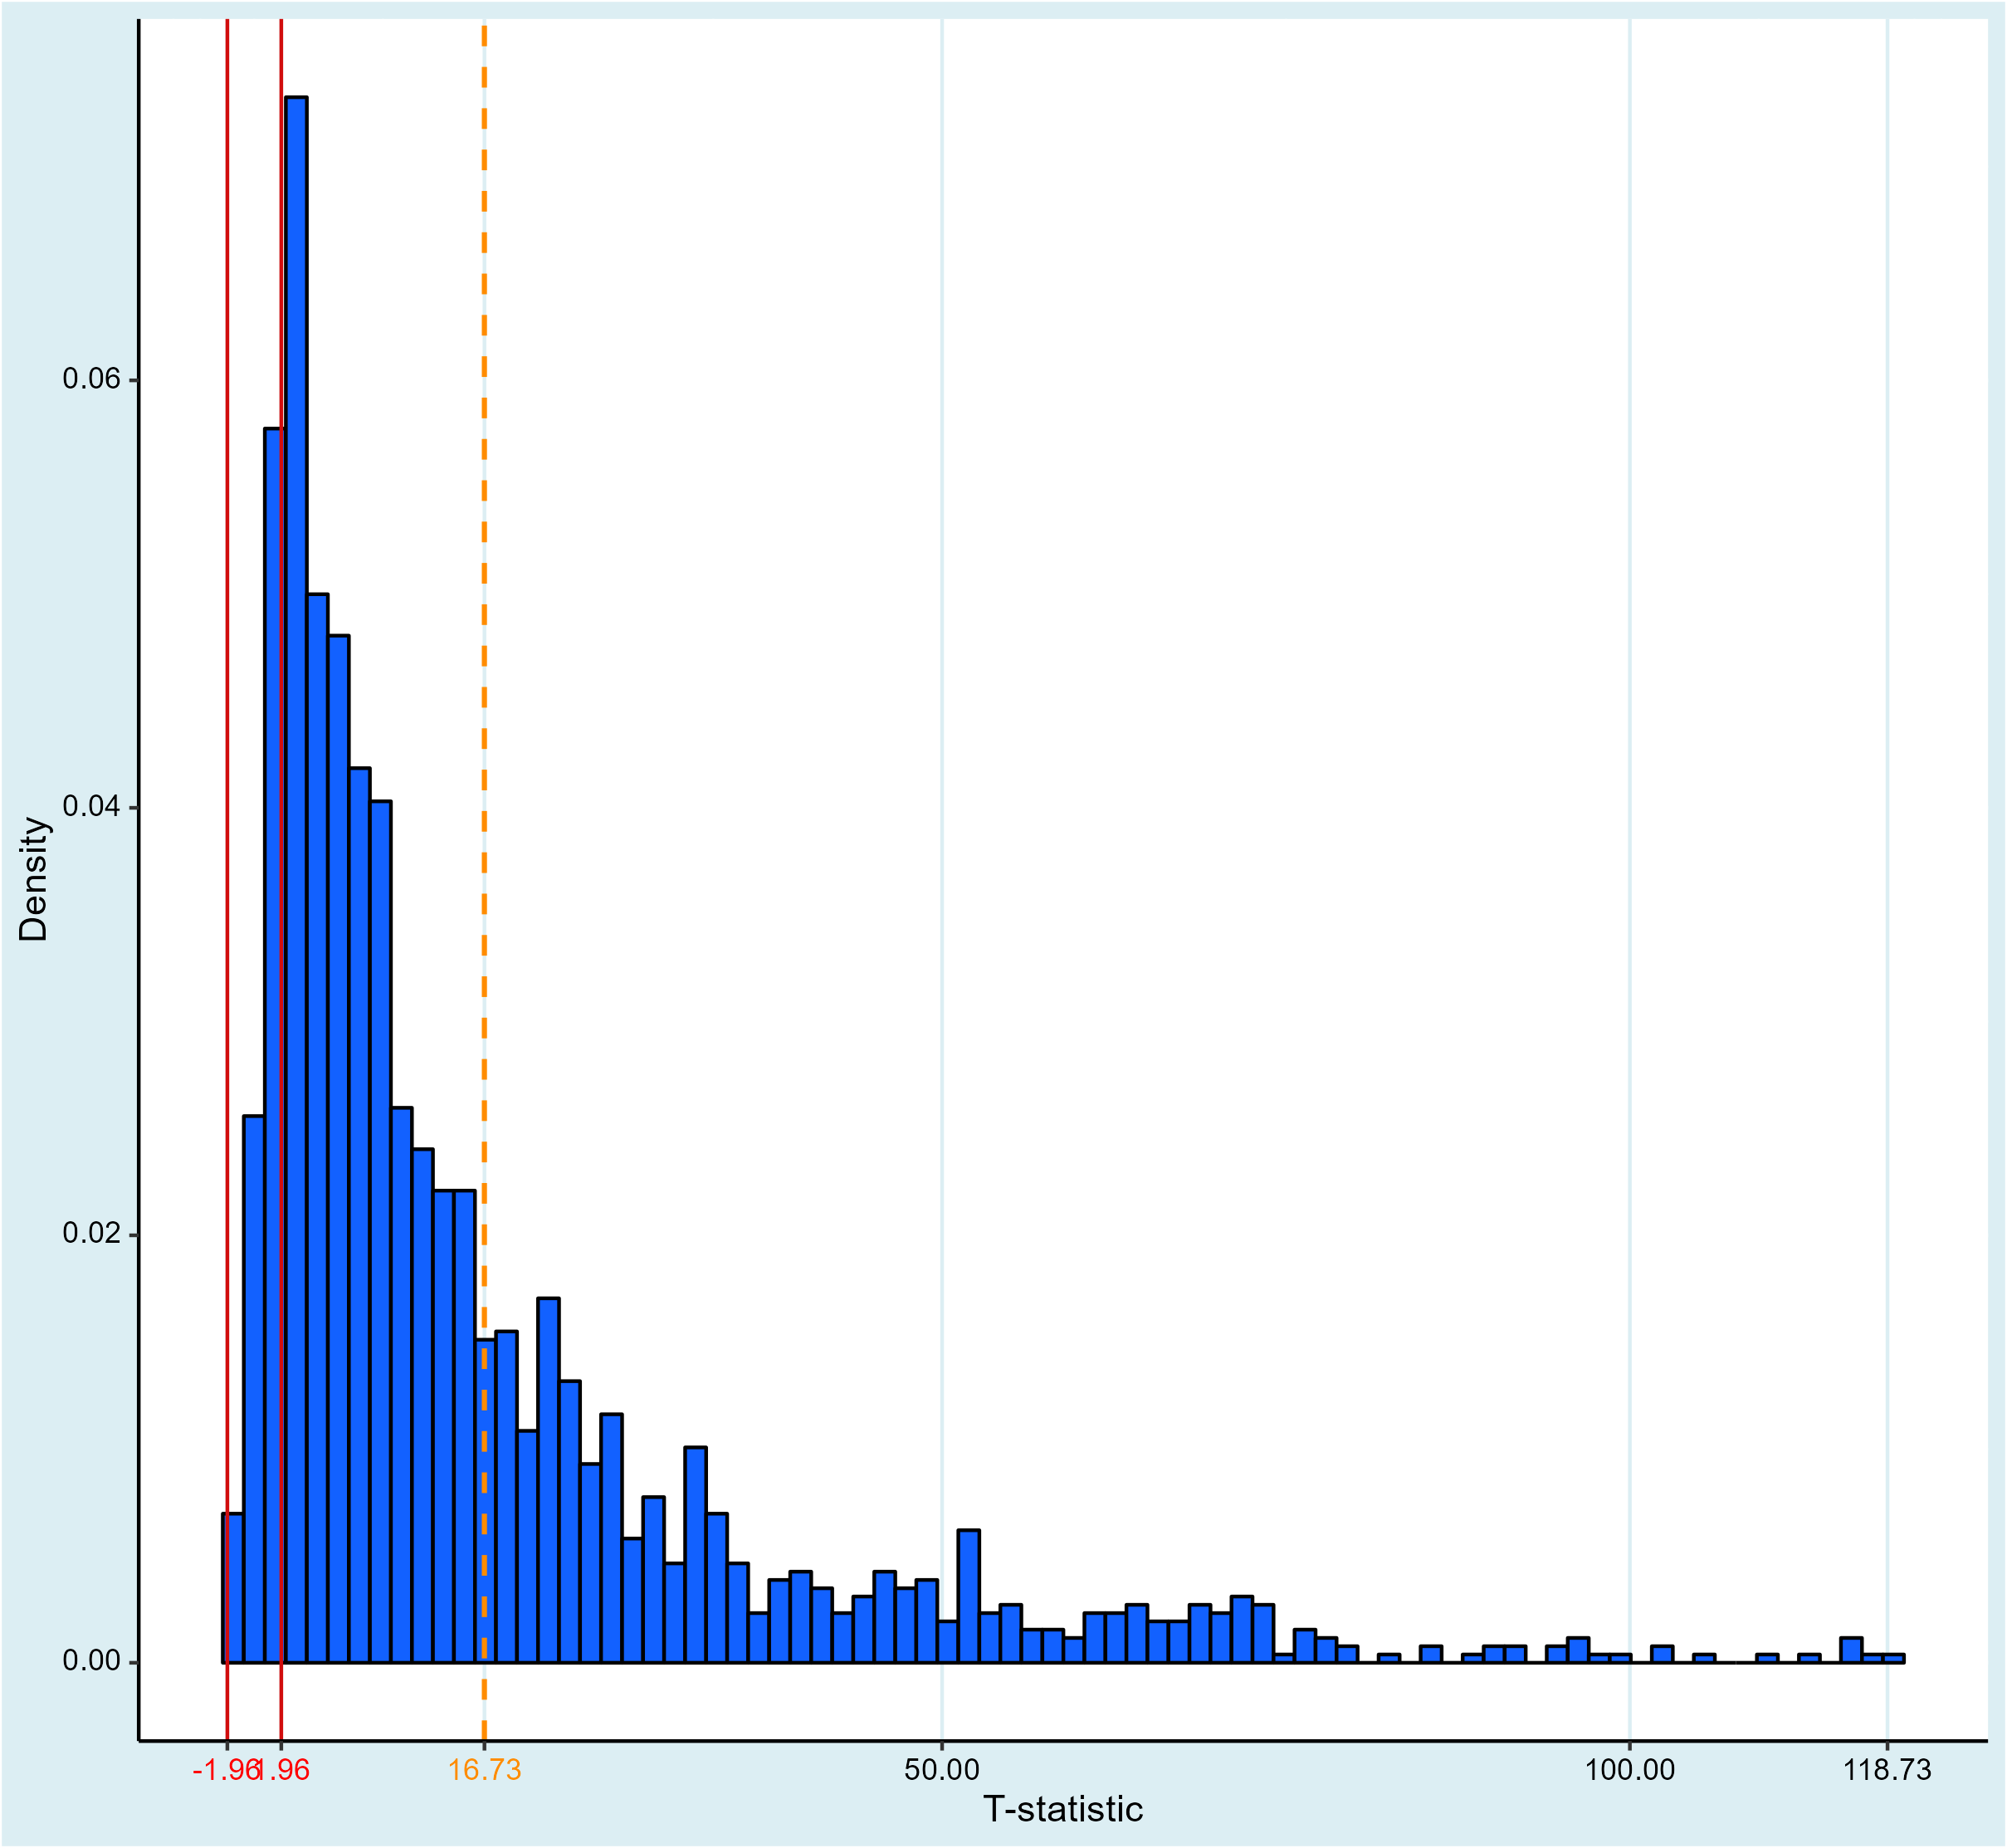
\includegraphics[width=0.95\linewidth]{Figures/t_hist.png}
  \end{subfigure}
  \begin{subfigure}[b]{0.45\textwidth}
    \caption{Close up around zero}
    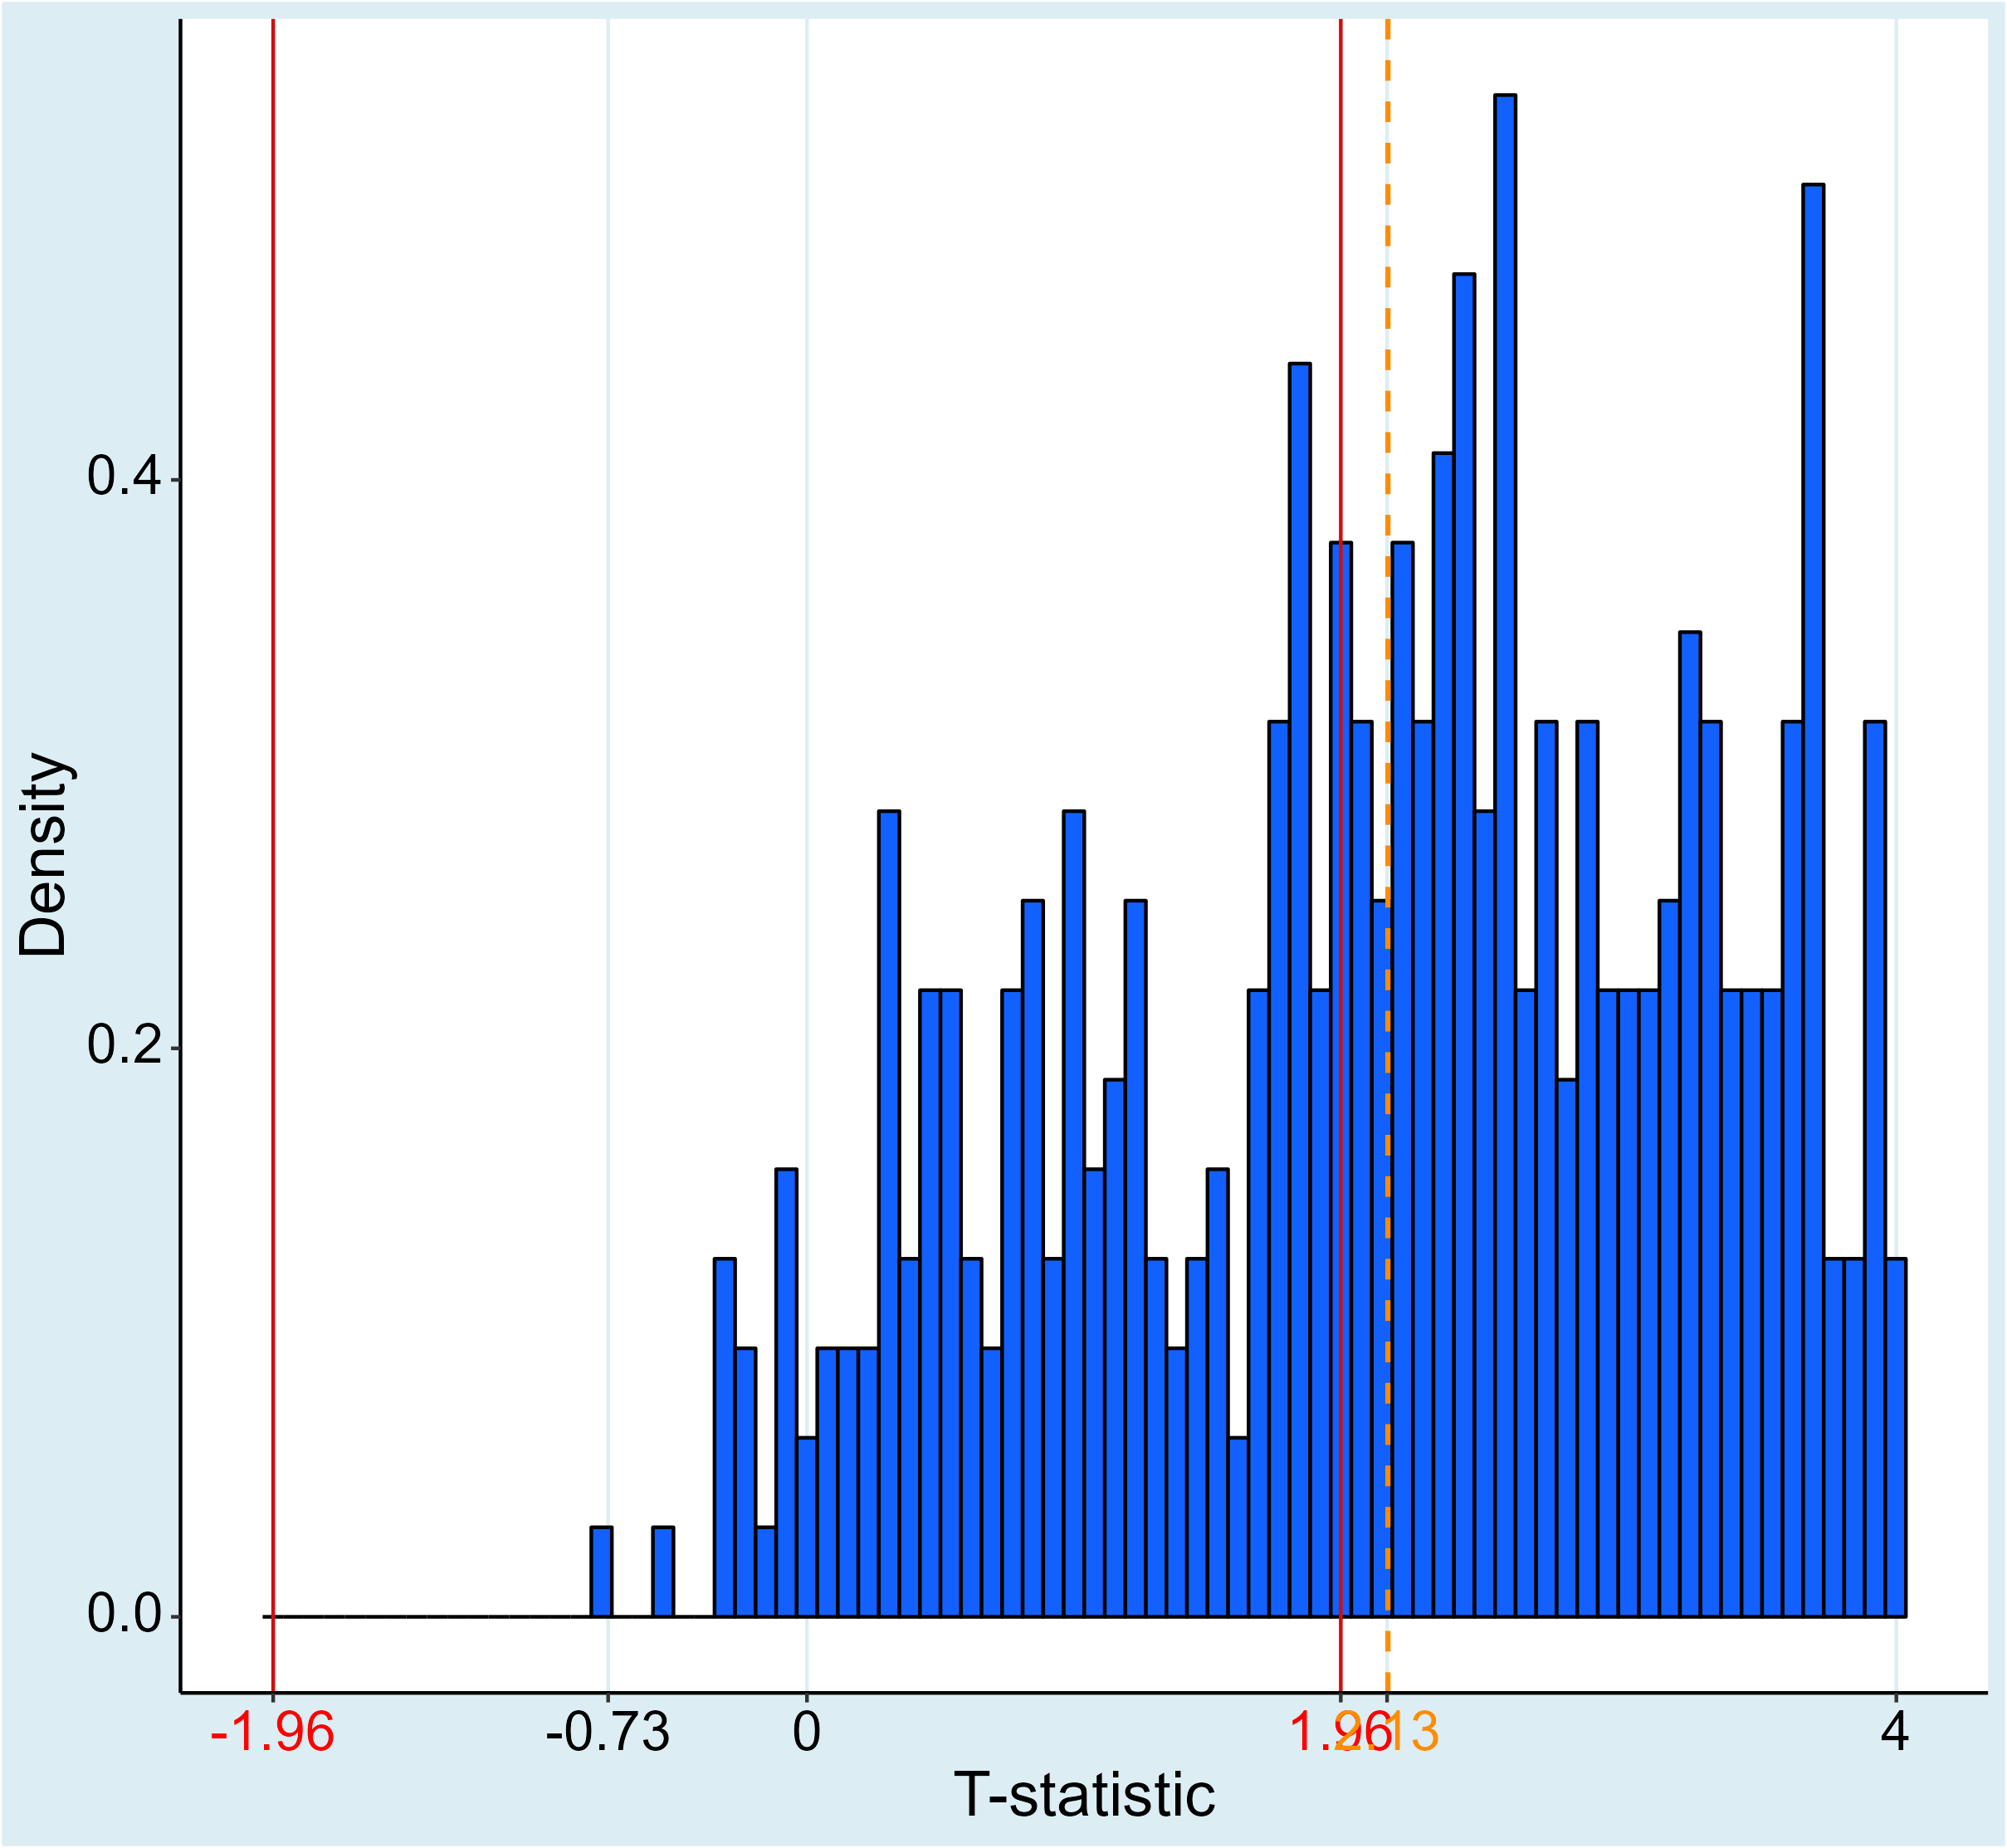
\includegraphics[width=0.95\linewidth]{Figures/t_hist_closeup.png}
  \end{subfigure}
  \captionsetup{width=0.85\textwidth, font = scriptsize}
  \caption*{\emph{Note:} The figure depicts the distribution of t-statistics associated with estimates within the dataset. Plot (a) shows all t-statistics in the dataset, while plot (b) focuses on a close up view around 0. The two red lines mark the critical significance values -1.96 and 1.96 (from left to right) at the 95\% confidence level. The dotted orange line represents the mean t-statistic within the data. Outliers are hidden for clarity of presentation, but we included them in the calculations.}
\end{figure}


% Results of Caliper tests
\begin{table}[!htbp]
  \centering
  \footnotesize
  \singlespace
  \caption{Caliper tests at values 1.645, 1.96 and 2.58}
  \label{tab:caliperA}
  \begin{tabular}{
      @{\hskip\tabcolsep\extracolsep}
      l
      *{3}{c}
      @{}
    }
    \toprule
    \multicolumn{1}{l}{}                                     &
    \multicolumn{1}{c}{\centering{\textbf{Threshold 1.645}}} &
    \multicolumn{1}{c}{\centering{\textbf{Threshold 1.96}}}  &
    \multicolumn{1}{c}{\centering{\textbf{Threshold 2.58}}}                                   \\
    \midrule
    Caliper width 0.05                                       & 0.517*** & 0.243*** & 0.152*** \\
    \emph{\hspace{0.2cm}SE}                                  & (0.084)  & (0.063)  & (0.046)  \\
    \emph{\hspace{0.2cm}Observations}                        & 7        & 17       & 18       \\
    \addlinespace[0.5em]
    Caliper width 0.1                                        & 0.467*** & 0.23***  & 0.183*** \\
    \emph{\hspace{0.2cm}SE}                                  & (0.069)  & (0.051)  & (0.037)  \\
    \emph{\hspace{0.2cm}Observations}                        & 13       & 25       & 28       \\
    \addlinespace[0.5em]
    Caliper width 0.15                                       & 0.483*** & 0.269*** & 0.186*** \\
    \emph{\hspace{0.2cm}SE}                                  & (0.042)  & (0.041)  & (0.028)  \\
    \emph{\hspace{0.2cm}Observations}                        & 26       & 37       & 45       \\
    \bottomrule
    \multicolumn{4}{>{\scriptsize}p{0.9\linewidth}}{\emph{Note:} The table shows the results of three sets of Caliper tests by \cite{gerber2008caliper} These sets are carried out around t-statistic thresholds of 1.645, 1.96 and 2.58, which correspond to the 1\%, 5\%, and 10\% t-statistic significance levels. Caliper width denotes the width of the interval around the t-statistic, e.g., Caliper width 0.05 for threshold 1.96 means $t\in<1.91;2.01>$. A test statistic of 0.243 means that roughly 74\% of estimates appear above the threshold and roughly 26\% below it. SE = Standard Error. Observations = Total number of observations in the interval around the threshold. Standard errors, clustered at the study level, are included in parentheses.}
  \end{tabular}
\end{table}


Two quick notes about the results are in order. First, there are very few (only 34 out of the 1754 observations) estimates with negative t-statistics. Looking at the distribution from a purely statistical standpoint, it appears peculiar that the other 1730 are all associated with a positive t-statistic. From a practical perspective, however, this makes a lot of sense if we presume that the true effect indeed lies around 7\%. This assumption appears quite feasible, given the consistency of the tests carried out in the previous sections.

The second note should be addressed to the results of the Caliper tests. The jumps around thresholds could be described as \textit{striking}, \textit{considerable}, and \textit{mild}, talking about the 1\%, 5\%, and 10\% thresholds, respectively. Speaking more bluntly, the words \textit{high}, \textit{medium}, and \textit{low} could be used. The t-statistics just above the thresholds of 1.645 and 1.96 are being over-reported in the data sample to some degree. So far, we have obtained somewhat skeptical views on publication bias presence in the dataset, but perhaps these thresholds could represent initial tangible indications of reporting misbehavior.

\section{Novel Tests for Detecting Publication Bias}
\label{sec:phacking}

As the last chapter of my hunt for publication bias, I present three new methods that further explore the issue of publication bias. The first two methods deal with p-hacking and have been developed very recently. They are, in order, the Elliott tests by \cite{elliott2022hacking} and the \ac{MAIVE} estimator by \cite{irsova2023maive}. While the former paper analyzes the distribution of p-values across different studies, the latter focuses on the issue of spurious regression and how p-hacking precision can produce biased results. As the last new method, I add \ac{RoBMA} \citep{maier2022robust}, a technique that can produce results of unparalleled quality and precision \citep{bartovs2023robust}.


% p-hacking tests
\begin{table}[!b]
  \centering
  \footnotesize
  \singlespace
  \caption{P-hacking tests}
  \label{tab:p-hacking}
  \begin{tabular}
    {
      @{\hskip\tabcolsep\extracolsep}
      l
      *{2}{c}
      @{}
    }
    \toprule
    \multicolumn{3}{l}{\textit{Panel A: P-hacking tests by \cite{elliott2022hacking}}}                                                             \\
    \multicolumn{1}{l}{}                                                      &
    \multicolumn{1}{p{4cm}}{\centering{\textbf{Test for non-increasingness}}} &
    \multicolumn{1}{p{4cm}}{\centering{\textbf{Test for monotonicity and bounds}}}                                                                 \\
    \midrule
    p-value                                                                   & 0.819                                                      & 0.871 \\
    Observations ($p\leq0.1$)                                                 & 1,610                                                      & 1,610 \\
    Total observations                                                        & 1,754                                                      & 1,754 \\
    \addlinespace[0.1em]
    \hline
    \addlinespace[0.5em]
    \multicolumn{3}{l}{\textit{Panel B: MAIVE estimator \citep{irsova2023maive}}}                                                                  \\
                                                                              & \multicolumn{1}{c}{\centering{\textbf{MAIVE coefficient}}} &       \\

    \midrule
    Coefficient                                                               & 5.736***                                                   &       \\
    Standard Error                                                            & (0.460)                                                    &       \\
    Observations                                                              & 1,754                                                      &       \\
    F-test                                                                    & 12.491                                                     &       \\
    \bottomrule
    \multicolumn{3}{>{\scriptsize}p{0.9\linewidth}}{\emph{Note:} This table shows the results of two techniques that detect p-hacking. Panel A shows the results of p-hacking tests by \cite{elliott2022hacking}, namely the histogram-based test for non-increasingness and the histogram-based test for monotonicity and bounds. Panel B reports the results of the spurious precision robust approach using the MAIVE estimator by \cite{irsova2023maive}. F-test = Test statistic of the IV first step F-test. Cluster-robust standard errors are used in the MAIVE estimation. These are reported in parentheses. ***p<0.01, **p<0.05, *p<0.1}
  \end{tabular}
\end{table}

First, let us talk about the Elliott tests. \cite{elliott2022hacking} propose an approach where \textit{no p-hacking in the literature} is considered as a null, and using a set of general assumptions, they test this hypothesis against an alternative of \textit{p-hacking in the literature}. The p-curves for various subsets of the true effects should be non-increasing and continuous, providing p-hacking is absent. For p-values based on t-tests, the authors then devise a new set of assumptions under which the lack of p-hacking should lead to a monotonous form of the p-curve. The advantage of the method lies in the fact that no threshold for the t-statistic needs to be specified; the technique only focuses on the p-curves. In my case, I present the results of the two tests I vaguely described - the test for non-increasingness of the p-curve and the test for monotonicity and bounds. With sufficiently low p-values, we could reject the null hypothesis of no p-hacking, but that is not the case in my dataset. Both tests yield p-values over 0.8, so there is insufficient evidence to reject the null in favor of the alternative (p-hacking).

Next, the \ac{MAIVE} estimator developed by \cite{irsova2023maive}. The authors argue that precision, one of the critical metrics in meta-analytic research, is prone to p-hacking. In their paper, \cite{irsova2023maive} raise several points of concern regarding the metric. First, the author must calculate the metric using reported standard errors; this makes the calculation easily 'p-hackable.' Second, even small amounts of p-hacking can profoundly impact the results. Precision is often used as a weighting metric in methods such as linear tests, plus it holds a vital role as one of the main axes of the funnel plot. As a remedy for this, \cite{irsova2023maive} propose a new estimator utilizing the instrumental variable approach (\ac{MAIVE}), where the reported variance is instrumented using the inverse sample size. This approach should help mitigate the impact of spurious precision in the data. This estimator suggests around 5.7\% percent returns to education, a figure lower than any of the tests conducted thus far. The F-statistic of around 12.5 then shows the inverse sample size to be a good instrument for reported variance. The results of both p-hacking tests are shown in \autoref{tab:p-hacking}.


%RoBMA
\begin{table}[!htbp]
  \centering
  \footnotesize
  \singlespace
  \caption{Robust Bayesian Model Averaging}
  \label{tab:robma}
  \begin{tabular}{
      l
        *{4}{c}
    }
    \toprule
    \multicolumn{5}{l}{\textit{Panel A: Model-averaged estimates}}                                \\
                                                         &
    \multicolumn{1}{c}{\centering{\textbf{Mean}}}        &
    \multicolumn{1}{c}{\centering{\textbf{Median}}}      &
    \multicolumn{1}{c}{\centering{\textbf{0.025}}}       &
    \multicolumn{1}{c}{\centering{\textbf{0.975}}}                                                \\
    \midrule
    Coefficient                                          & 7.123** & 7.122** & 6.946** & 7.299**  \\
    Standard Error                                       & (3.506) & (3.504) & (3.373) & (3.645)  \\
    Observations                                         & 1,754   & 1,754   & 1,754   & 1,754    \\
    \addlinespace[0.1em]
    \hline
    \addlinespace[0.5em]
    \multicolumn{5}{l}{\textit{Panel B: Summary of individual components}}                        \\
                                                         &
    \multicolumn{1}{c}{\centering{\textbf{Models}}}      &
    \multicolumn{1}{c}{\centering{\textbf{Prior Prob.}}} &
    \multicolumn{1}{c}{\centering{\textbf{Post. Prob.}}} &
    \multicolumn{1}{c}{\centering{\textbf{Inclusion BF}}}                                         \\
    \midrule
    Effect                                               & 2/4     & 0.500   & 1.000   & $\infty$ \\
    Heterogeneity                                        & 2/4     & 0.500   & 1.000   & $\infty$ \\
    Bias                                                 & 0/4     & 0.500   & 0.000   & 0.000    \\
    \bottomrule
    \multicolumn{5}{>{\scriptsize}p{0.85\linewidth}}{\emph{Note:} This table shows the Robust Bayesian Model Averaging method by \cite{maier2022robust}. Panel A contains four descriptive statics of the estimates obtained from model-averaging - mean, median, 2.5th quantile, and 97.5th quantile. Standard errors are reported in parentheses. In Panel B, the summary of three individual components is displayed - effect, heterogeneity, and publication bias. Models = Probability of each model assuming a given individual component. Prior Prob. = Prior Probability. Post. Prob. = Posterior Probability. Inclusion BF = Inclusion Bayes Factor. ***p<0.01, **p<0.05, *p<0.1}
  \end{tabular}
\end{table}


The last of the procedures exploring publication bias is the \ac{RoBMA} by \cite{maier2022robust}. The idea lies in estimating multiple meta-analytic models and combining them using Bayesian model averaging. Each model is assigned a different weight, and individual components, such as the presence or absence of an effect, are tested using Bayes factors. In \autoref{tab:robma}, I present two panels: the first panel displays the model-averaged estimates of the effect, while the second panel summarizes the individual components - effect, heterogeneity, and publication bias. The effect estimates propose a mildly confident claim that the effect lies just above 7\% percent, which is slightly more positive than the estimates of both linear and non-linear models. Among the four models used to estimate individual components\footnote{I used the base specification of the \textit{RoBMA} method. For the list of models and other parameters used, see the source code of the method, available \href{https://github.com/FBartos/RoBMA/}{here}.}, the probability of a model assuming the presence of effect or heterogeneity is 2/4 (50\%), while for publication bias it is 0/4 (0\%).


To summarize, all models agree that schooling positively affects log wage (rate of returns to an additional year of schooling of 5.7-9.5\%), and most suggest it lies somewhere between 6 and 7 percent. The vast majority of results associated with these techniques are also highly statistically significant. As for publication bias, the story is a bit more tangled. Some linear and non-linear methods argue for its presence, while others are against it. Even when relaxing the assumption of exogeneity of the standard error, the results appear mixed. Novel methods almost uniformly suggest the lack of publication bias, apart from \ac{MAIVE}, which predicts lower returns to education when instrumenting for study variance. Lastly, the Caliper tests show that sizeable jumps exist in the distribution of t-statistics around 1\% and 5\% significance levels. Perhaps too many cooks spoil the broth, so a single interpretation appears unfeasible, and I would suggest considering the results of the presented methods individually.
\chapter{Heterogeneity}
\label{chap:five}
% grammar checked (07-26)

Thus far, my analysis has focused primarily on the relationship between the true effect and its standard error. Several methods from the previous chapter, such as the \ac{IV} regression, p-uniform*, or \ac{RoBMA}, provided us with a quick glimpse into the topic of systematic heterogeneity. However, none delivered a more complex overview of the data's nature. This chapter aims to do precisely that - delve deeper into the study design and search for systematic patterns that may reveal more about the behavior of the effect. For this purpose, I will utilize two methods, \ac{BMA} and \ac{FMA}. These should help me identify the influence of different variables on the effect behavior and quantitatively capture the magnitude of this influence. Before constructing any models, however, it is crucial to explain and explore the dataset structure first.

\section{Variables}
\label{sec:variables}

I constructed the dataset aiming to comprehensively capture the most important categories that define the context of the collected data and the studies they come from. As such, I identified six categories, which I named as follows: the actual estimates along with their descriptive statistics, estimate characteristics, data characteristics, spatial/structural variation, estimation method, and publication characteristics. Across these six categories, I collected 37 distinct variable groups. Note that a group here could mean either a standalone variable (i.e., data year) or a group of variables (i.e., low/middle/high-income country). In the latter case, the variable groups consist either of dummies, or ratios, such as the ratio of subjects living in an urban area. The list of all quantifiable, relevant variables can be found in \autoref{tab:var}. To keep visual clarity, I excluded variables that could not be easily quantified, such as the country where the study was conducted, or variables irrelevant to the effect behavior explanation, such as observation id.

%BMA+FMA table
\begin{singlespace}
\begin{scriptsize}
\begin{longtable}{
@{\hskip\tabcolsep\extracolsep\fill}
l
%p{0.25\hsize}
p{0.55\hsize}
cc
@{}
} %0.15 0.65
\caption{Definition and summary statistics of regression variables}  \label{tab:var}\\
\toprule
  \multicolumn{1}{l}{Variable} &   \multicolumn{1}{l}{Description} &         \multicolumn{1}{c}{Mean} &           \multicolumn{1}{c}{SD} \\
\midrule
\endfirsthead
\caption[]{Definition and summary statistics of regression variables (continued)}\\
\toprule
  \multicolumn{1}{l}{Variable} &   \multicolumn{1}{l}{Description} &         \multicolumn{1}{c}{Mean} &           \multicolumn{1}{c}{SD} \\
\midrule
\endhead
\bottomrule
\multicolumn{4}{r}{{\scriptsize Continued on next page}} \\
\endfoot
\endlastfoot
                 Effect &                                                                                       The effect of an additional year of schooling on logarithmic wage. &    7.476 &  4.439 \\
         Standard Error &                                                                                                                   The standard error of the main effect. &    1.284 &  1.693 \\
    \midrule
    
\multicolumn{4}{l}{\emph{Estimate characteristics}}\\	
         Estimate: City &                                                                                  =1 if the estimates within the study can be aggregated on a city level. &    0.119 &  0.323 \\
   Estimate: Sub-region &                                                                           =1 if the estimates within the study can be aggregated on a subregional level. &    0.099 &  0.299 \\
       Estimate: Region &                                                                              =1 if the estimates within the study can be aggregated on a regional level. &    0.309 &  0.462 \\
      Estimate: Country &                                                                               =1 if the estimates within the study can be aggregated on a country level. &    0.395 &  0.489 \\
    Estimate: Continent &                                           =1 if the estimates within the study can not be aggregated on a country level or smaller (reference category). &    0.079 &  0.269 \\
    \midrule 
    
\multicolumn{4}{l}{\emph{Data characteristics}}\\	
             Study Size &                                                                                       The logarithm of the number of estimates collected from the study. &    2.942 &  0.637 \\
      Yrs. of Schooling &                                                                                       The average number of years of schooling attained by the subjects. &   11.116 &  3.461 \\
     Yrs. of Experience &                                                                                      The average number of years of experience attained by the subjects. &   18.351 &  7.450 \\
       Education: Years &                                                                                                                 =1 if authors report schooling in years. &    0.634 &  0.482 \\
      Education: Levels &                                                       =1 if the authors report schooling in levels (e.g., attained college degree) (reference category). &    0.366 &  0.482 \\
       Wage: Log Hourly &                                                                                       =1 if the dependent variable in the regression is log hourly wage. &    0.531 &  0.499 \\
        Wage: Log Daily &                                                                              =1 if the dependent variable in the regression is log daily or weekly wage. &    0.095 &  0.293 \\
      Wage: Log Monthly &                                                                                      =1 if the dependent variable in the regression is log monthly wage. &    0.211 &  0.408 \\
  Wage: Annual Earnings &                                                      =1 if the dependent variable in the regression is a log of mean annual earnings (reference category). &    0.162 &  0.369 \\
             Micro Data &                                                                                                                         =1 if the study uses micro-type data. &    0.177 &  0.382 \\
            Survey Data &                                                                                                                 =1 if the study uses data from a survey. &    0.534 &  0.499 \\
 National Register Data &                                                                                 =1 if the study uses data from a national register (reference category). &    0.289 &  0.453 \\
   Cross-sectional Data &                                                                                                               =1 if the study uses cross-sectional data. &    0.361 &  0.481 \\
             Panel Data &                                                                                                    =1 if the study uses panel data (reference category). &    0.639 &  0.481 \\
              Data Year &                                                                                               The logarithm of the average year of the study's time span &    7.599 & 0.006 \\
    \midrule 
    
\multicolumn{4}{l}{\emph{Spatial/structural variation}}\\
           No Education &                                                                              The percentage of subjects that attained no education (reference category). &    0.126 &  0.148 \\
      Primary Education &                                                                                         The percentage of subjects that attained only primary education. &    0.177 &  0.151 \\
    Secondary Education &                                                                                       The percentage of subjects that attained only secondary education. &    0.388 &  0.196 \\
       Higher Education &                                                                                   The percentage of subjects that attained higher education. &    0.309 &  0.247 \\
           Wage Earners &                                            The ratio of wage earners to self-employed subjects in the study ( = 1 if wage earner, = 0 if self-employed). &    0.837 &  0.205 \\
          Self-Employed &                       The ratio of self-employed to wage earners subjects in the study ( = 1 if self-employed, = 0 if wage earner) (reference category). &    0.163 &  0.205 \\
           Gender: Male &                                                                         The ratio of male to female subjects in the study ( = 1 if male, = 0 if female). &    0.650 &  0.350 \\
         Gender: Female &                                                    The ratio of female to male subjects in the study ( = 1 if female, = 0 if male) (reference category). &    0.350 &  0.350 \\
        Sector: Private &                                                            The ratio of private to public sector workers ( = 1 if private sector worker, = 0 if public). &    0.596 &  0.163 \\
         Sector: Public &                                       The ratio of public to private sector workers ( = 1 if public sector worker, = 0 if private) (reference category). &    0.404 &  0.163 \\
   Ethnicity: Caucasian &                                                           The ratio of Caucasian to non-Caucasian subjects in the study ( = 1 if Caucasian, = 0 if not). &    0.227 &  0.419 \\
       Ethnicity: Other &                            The ratio of non-Caucasian to Caucasian subjects in the study ( = 1 if non-Caucasian, = 0 if Caucasian) (reference category). &    0.773 &  0.419 \\
          Sector: Rural &                                                                                The ratio of rural to urban workers ( = 1 if rural worker, = 0 if urban). &    0.297 &  0.191 \\
          Sector: Urban &                                                           The ratio of urban to rural workers ( = 1 if urban worker, = 0 if rural) (reference category). &    0.703 &  0.191 \\
    Reg: Advanced Econ. &                                                                      =1 if the study was conducted in a country with an advanced economy. (reference group) &    0.498 &  0.500 \\
Reg: E. Asia \& Pacific &                                                                                       =1 if the study was conducted in the East Asia and Pacific region. &    0.213 &  0.409 \\
Reg: Europe and C. Asia &                                                                                     =1 if the study was conducted in the Europe and Central Asia region. &    0.115 &  0.319 \\
 Reg: Lat. Am. and Car. &                                                                                 =1 if the study was conducted in the Latin America and Caribbean region. &    0.004 &  0.063 \\
Reg: M. East and N. Af. &                                                                                =1 if the study was conducted in the Middle East and North Africa region. &    0.043 &  0.202 \\
      Reg: South Africa &                                                                                               =1 if the study was conducted in the South African region. &    0.088 &  0.283 \\
   Reg: Sub Sah. Africa &                                                                                       =1 if the study was conducted in the region of Sub-Saharan Africa. &    0.106 &  0.308 \\
           Income: High &                                                                              =1 if the study was conducted in a high-income country (reference category) &    0.507 &  0.500 \\
         Income: Middle &                                                                                                 =1 if the study was conducted in a middle-income country &    0.434 &  0.496 \\
            Income: Low &                                                                                                    =1 if the study was conducted in a low-income country &    0.059 &  0.236 \\
     Median Expenditure &                                                                                  The logarithm of the median expenditure in the country in a given year. &    8.584 &  1.420 \\
           Minimum Wage &                                                                                        The logarithm of the minimum wage in the country in a given year. &    5.853 &  1.536 \\
 Academic Freedom Index &                                                                                     The academic freedom index reported for the country in a given year. &    0.712 &  0.266 \\
               Mean Age &                                                                                                        The logarithm of the average age of the subjects. &    3.575 &  0.200 \\
    \midrule 
    
\multicolumn{4}{l}{\emph{Estimation method}}\\    
            Method: OLS &                                                                                                            =1 if the authors use Ordinary least squares (reference category). &    0.664 &  0.473 \\
      Method: Cohort/FE &                                                                                           =1 if the authors use Cohort-type or Fixed-effects estimation. &    0.058 &  0.234 \\
           Method: 2SLS &                                                                                                =1 if the authors use Two-Stage least squares estimation. &    0.095 &  0.294 \\
        Method: Heckman &                                                                                  =1 if the authors use Two-step estimation \citep{heckman1974empirical}. &    0.062 &  0.240 \\
         Method: Probit &                                                                                                                 =1 if the authors use Probit estimation. &    0.022 &  0.147 \\
             Method: IV &                                                                            =1 if the authors use Instrumental variables estimation. &    0.111 &  0.314 \\
        Ability: Direct &                                                                                    =1 if the authors include a direct measure of ability in their study. &    0.135 &  0.341 \\
       Ability: Proxied &                                                                                                =1 if the authors use a proxy for ability in their study. &    0.204 &  0.403 \\
  Ability: Uncontrolled &                                                                 =1 if the authors acknowledge but do not control for ability in any way in their study. &    0.425 &  0.494 \\
   Ability: Unmentioned &                                                                   =1 if the authors do not mention ability anywhere in their study (reference category). &    0.223 &  0.417 \\
           Control: Age &                                                                                                     =1 if the authors control for age in the regression. &    0.344 &  0.475 \\
       Control: Age$^2$ &                                                                                   =1 if the authors control for age in the quadratic form in the regression. &    0.275 &  0.447 \\
    Control: Experience &                                                                                              =1 if the authors control for experience in the regression. &    0.607 &  0.489 \\
Control: Experience$^2$ &                                                                            =1 if the authors control for experience in the quadratic form in the regression. &    0.512 &  0.500 \\
     Control: Ethnicity &                                                                                               =1 if the authors control for ethnicity in the regression. &    0.251 &  0.434 \\
        Control: Health &                                                                                                  =1 if the authors control for health in the regression. &    0.135 &  0.342 \\
        Control: Gender &                                                                                                  =1 if the authors control for gender in the regression. &    0.367 &  0.482 \\
      Control: Marriage &                                                                                                =1 if the authors control for marriage in the regression. &    0.361 &  0.480 \\
    Control: Occupation &                                                                              =1 if the authors control for the subjects' occupation in the regression. &    0.142 &  0.349 \\
    Control: Firm Char. &                                                                                    =1 if the authors control for firm characteristics in the regression. &    0.149 &  0.357 \\
          Control: Area &                                                                          =1 if the authors control for area type in the regression (e.g., urban, rural). &    0.418 &  0.493 \\
    Control: Macro Var. &                                                                                 =1 if the authors control for macroeconomic variables in the regression. &    0.347 &  0.476 \\
    \midrule
    
\multicolumn{4}{l}{\emph{Publication characteristics}}\\    
          Impact Factor &                            The logarithm of the Journal Citations Report impact factor of the study (as of January 2023; = 0 in case of no publication). &   -0.906 &  1.533 \\
              Citations & The logarithm of the mean number of Google Scholar citations received per year since the appearance of the study in Google Scholar (as of January 2023). &    4.029 &  2.177 \\
       Study: Published &                                                                                                              =1 if the study was published in a journal. &    0.764 &  0.425 \\
     Study: Unpublished &                                                                                     =1 if the study was not published in a journal (reference category). &    0.236 &  0.425 \\
     Publication Year &  The logarithm of the years passed between this study's publication (or issuing) and the publication year of the earliest published study in the sample. & 3.332 & 0.339 \\

\bottomrule
   
 \multicolumn{4}{>{\scriptsize}p{0.95\linewidth}}{\emph{Note:} This table presents the summary statistics and descriptions for various study characteristics eligible for inclusion in Bayesian Model Averaging. Variables marked as \textit{reference categories} were automatically excluded from the procedure, as this would create a dummy variable trap. SD = standard deviation, OLS = Ordinary Least Squares, FE = Fixed Effects, 2SLS = 2 Stage Least Squares, IV = Instrumental Variable.}
\end{longtable}
\end{scriptsize}
\end{singlespace}

Let us take a closer look at five of the six\footnote{The statistical properties of the estimate have already been described in \autoref{chap:three}.} variable categories and try to understand the reasoning behind my choices of this particular variable setup.

\subsection{Estimate Characteristics}
\label{subsec:estimate_char}

There are only a handful of variables that I identified as vital as far as effect characteristics are concerned. Moreover, variables such as the number of observations, or degrees of freedom, are not telling enough to be included in the model averaging. As such, the only full-fledged variable group included in this category is the estimate type, when divided into the size of the region. The estimates of over 70\% of studies in the dataset can be clustered into regional or country levels. Examples of such studies include \cite{walker2008college, fang2012returns}, or \cite{angrist1991compulsory}. Sporadically \citep{krafft2019what, chanis2021tell}, the authors focus on the city/sub-region level estimates or aggregate their results at a level of a continent or a group of countries.

\subsection{Data Characteristics}
\label{subsec:data_char}

Two variables are perhaps the most important in the category of data characteristics - \textit{years of schooling} and \textit{years of experience}. These represent the founding blocks of the Mincer equation and can be linked together using the age of subjects as described in \autoref{eq:potential_exp}. Across all studies in the data, the average reported number of schooling years equals 11.116, while 18.351 represents the average reported experience of subjects. Given that 781 observations in the data (roughly 44\% of all observations) are not directly reported, the \textit{years of experience} variable may be inflated by the calculation. Indeed, upon removing all observations that had to be manually calculated using \autoref{eq:potential_exp}, the average years of experience in the sample drops to 15.637. Nonetheless, to the best of my knowledge, there is no other way to circumvent this shortcoming. Consequently, I will use the reported number of 18.351 in further calculations. To see examples of studies that fail to report years of schooling and/or experience, see \cite{pischke2005zero, psacharopoulos1982earnings}, while for studies that report both, see \cite{belzil2002unobserved, girma2005heterogeneity}.

Another crucial variable captures how education is reported - years or levels\footnote{See \autoref{sec:effect_meaning} for more details about this classification.} In about two-thirds of all studies, years of attained education is used instead of the highest attained level (primary school, secondary school, etc.). It should be noted here that in cases a study reported both types, but the results captured the same outcome, I chose to collect only the number of years and discard the estimates in levels. This is to avoid collecting duplicate results. \cite{harmon2002returns} is an excellent example of a study that utilizes reporting of schooling years, while \cite{duraisamy2002changes} provides a counterexample.

The last variable worth a mention from this category is the variable denoting cross-section/panel data. Initially, I coded a short/long run variable under the \textit{estimate characteristics} that divided studies according to their run-time into those of length above and below one year. However, after the collection, I found that the cross-section/panel variable almost entirely captured this information, so I kept only this variable in the data. Nearly two-thirds of the collected experiments work with panel data such as longitudinal surveys (see \cite{harmon2003returns}). On the other hand, one-third of them deal with cross-sectional data (\cite{lemieux2001education} as an example).

The rest of the variables in this category is self-explanatory. For the complete list, see \autoref{tab:var}.

\subsection{Spatial/Structural Variation}
\label{subsec:spat_str_variation}

A whole array of variables that capture study variation are all coded under the category \textit{spatial/structural variation}. In most cases, this refers to either characteristics of the study subjects or the country in which the study is conducted. Pointing out a handful of crucial statistics that tie to these variables, we can see that most of the data sample consists of wage workers (83.7\%), 65\% of the subjects are male, 22.7\% come from the Caucasian ethnicity, 70.3\% live in the urban area, about half of them (49.8\%) come from a country with an advanced economy, and their average age is 35.69. To see the rest of the statistics, see \autoref{tab:var}.

Most of the choices regarding the variables themselves should be more or less straightforward. As such, I would like to focus on the calculation behind some of these instead. For example, the variables \textit{median expenditure} and \textit{minimum wage} are notably coded on the country-year level, meaning a data point exists for every unique country-year pair. This is to account for country-level heterogeneity, as well as inflation. Another variable, the \textit{academic freedom index}, is too coded in this way.

Some variables, such as the rural/urban sector, are set up as ratios. \cite{paweenawat2015private}, for example, report exactly 47.4\% of subjects that live in rural areas, and 57.6\% that live in urban ones. This variable structure allows us to retain more information while behaving as a simple dummy in case only one of the alternatives is present in the data, such as when all subjects live in a city. I also employ this ratio-type setup with multiple categories in the variable that denotes the highest attained education. Here, the choices are split between primary, secondary, and higher education, as well as no education. When the authors report only several of these but not all, such as in the case of \cite{chanis2021tell}, I set the remaining variable categories to 0.

A more complex issue arises when more data points are missing, however. As an example, 32.5\% of the 1754 studies do not report whether their subject pool consists of wage workers or self-employed individuals. 53.4\% then omit the information on area type (urban/rural), and 60.5\% fail to specify whether the subjects work in a private or a public sector. To run the model averaging, the dataset has to contain no missing points in the employed variables. As such, I resort to interpolation, whose specifics I explained earlier in \autoref{chap:three}.

\subsection{Estimation Method}
\label{subsec:estim_method}

Regarding the actual estimation of the Mincer equation, the practices literature can be explained by three major variable sub-categories. Firstly, the estimation method used by the studies. Two-thirds of studies in the dataset (66.4\%) use simple \ac{OLS} for the estimation, while the rest use one of several other methods, including the Fixed-effects, Probit model, Instrumental variable regression, or Two-stage least squares. Several studies, such as \cite{debrauw2008reconciling}, employ a two-step estimation described in \cite{heckman1974empirical}.

Secondly, the \textit{ability} variable, described in \autoref{chap:two}, is also coded here. We can see that 13.5\% of studies include ability directly in the regression, 20.4\% use a proxy of some kind, 42.5\% do not control for ability but are aware of it, and 22.3\% do not mention ability or ability bias in any way.

Lastly, I add information on whether a study controls for variables such as age, experience, ethnicity, health, gender, marital status, etc. Usually, such as in the case of \cite{girma2005heterogeneity} or \cite{harmon2002returns}, only one of the two variables of age and experience are included. On the other hand, the included variable comes very frequently with the squared term, as described in the original Mincer equation. As for the other controls, there seems to be no obvious pattern in the studies, and the authors appear to be choosing the controls arbitrarily based on their study goals, data availability, or personal preferences.

\subsection{Publication Characteristics}
\label{subsec:pub_characteristics}

The last of the variable categories that I chose to employ denotes various publication characteristics of the included studies. The number of Google Scholar citations, the year of publication, or the Journal Citations Report impact factor are among the handful of variables within this category. As described in \autoref{chap:three}, I collected all journal/study data at a single time point, namely in January 2023. Although it is possible that the status of several of the included studies changed from then, I still value direct comparability more than keeping the information up-to-date with the latest changes.

Interestingly, but perhaps not surprisingly, 76.4\% of studies within the sample were published in a journal, and the mean number of citations for a study comes up to 56.2. This relatively high figure ties directly to the fact that roughly a third of the dataset consists of studies identified by snowballing - an activity aimed at targeting the most relevant and well-established relevant papers on the topic. Understandably, all of these papers have attained publication status, or their credibility would not be established.

With the variable setup out of the way, we can move on and employ these variables in exploring the effect behavior in a more detailed way.

\section{Model Averaging}
\label{sec:bma}

With the large number of variables my dataset holds, it is a rather complex and no doubt challenging task to pick those that could explain the effect behavior the best. Indeed, traditional methods such as \ac{OLS} are prone to over-specification bias, so simply dumping all collected variables into a single model does not appear like the best approach. Is there a way, then, where we could somehow discern the importance of the collected variables without knowing anything about them a priori? One such technique, called \ac{BMA}, appears suitable for the task and is precisely what the following sections will focus on.

Pioneered over two decades ago in papers such as \cite{hoeting1999bayesian} or \cite{raftery1997bayesian}, the technique provides a balanced approach that considers a multitude of statistically plausible models and assigns different weights to them using the Bayes' theorem and posterior inclusion probabilities. As explained in \cite{hoeting1999bayesian} and \cite{amini2011bayesian}, the process then highlights the importance of each variable based on these weights. For the procedures employed in this thesis, it is crucial to understand two metrics - \ac{PMP} and \ac{PIP}. For each variable, \ac{PMP} denotes how well each model fits the data. In contrast, \ac{PIP} is the sum of posterior model probabilities across the models in which that variable is included. The higher \ac{PIP}, the higher the variable's importance for explaining the effect's behavior.

I use a combination of the default Zellner's g-prior and the dilution prior for this particular analysis. The choice of the former stems from the fact that this setup allows for more control over collinearity in the data, an issue that may arise with the high number of variables. In my case, the number of eligible individual variables fed into the process once is 52 once reference variables are removed, making the collinearity treatment seem wise. \footnote{Here, an individual variable refers to each sub-group of a dummy variable group or any other variable that contains multiple categories. For example, the highest achieved education variable, as explained in \autoref{subsec:spat_str_variation}, would account for four individual variables (none, primary, secondary, and higher).} To ensure the carried information is unique for every variable, I also check the variance inflation factors of the included variables. This check revealed the sound design of the dataset, as all 52 variables, when lumped into a single model, hold a variance inflation factor no larger than 10. As for other parts of the setup, the last point of interest lies perhaps in the choice of the sampler, where I choose to use the default Markov Chain Monte Carlo algorithm \citep{zeugner2015bayesian}.

\begin{figure}[!t]
\begin{center}
\caption{Bayesian model averaging results}
\label{fig:BMA}
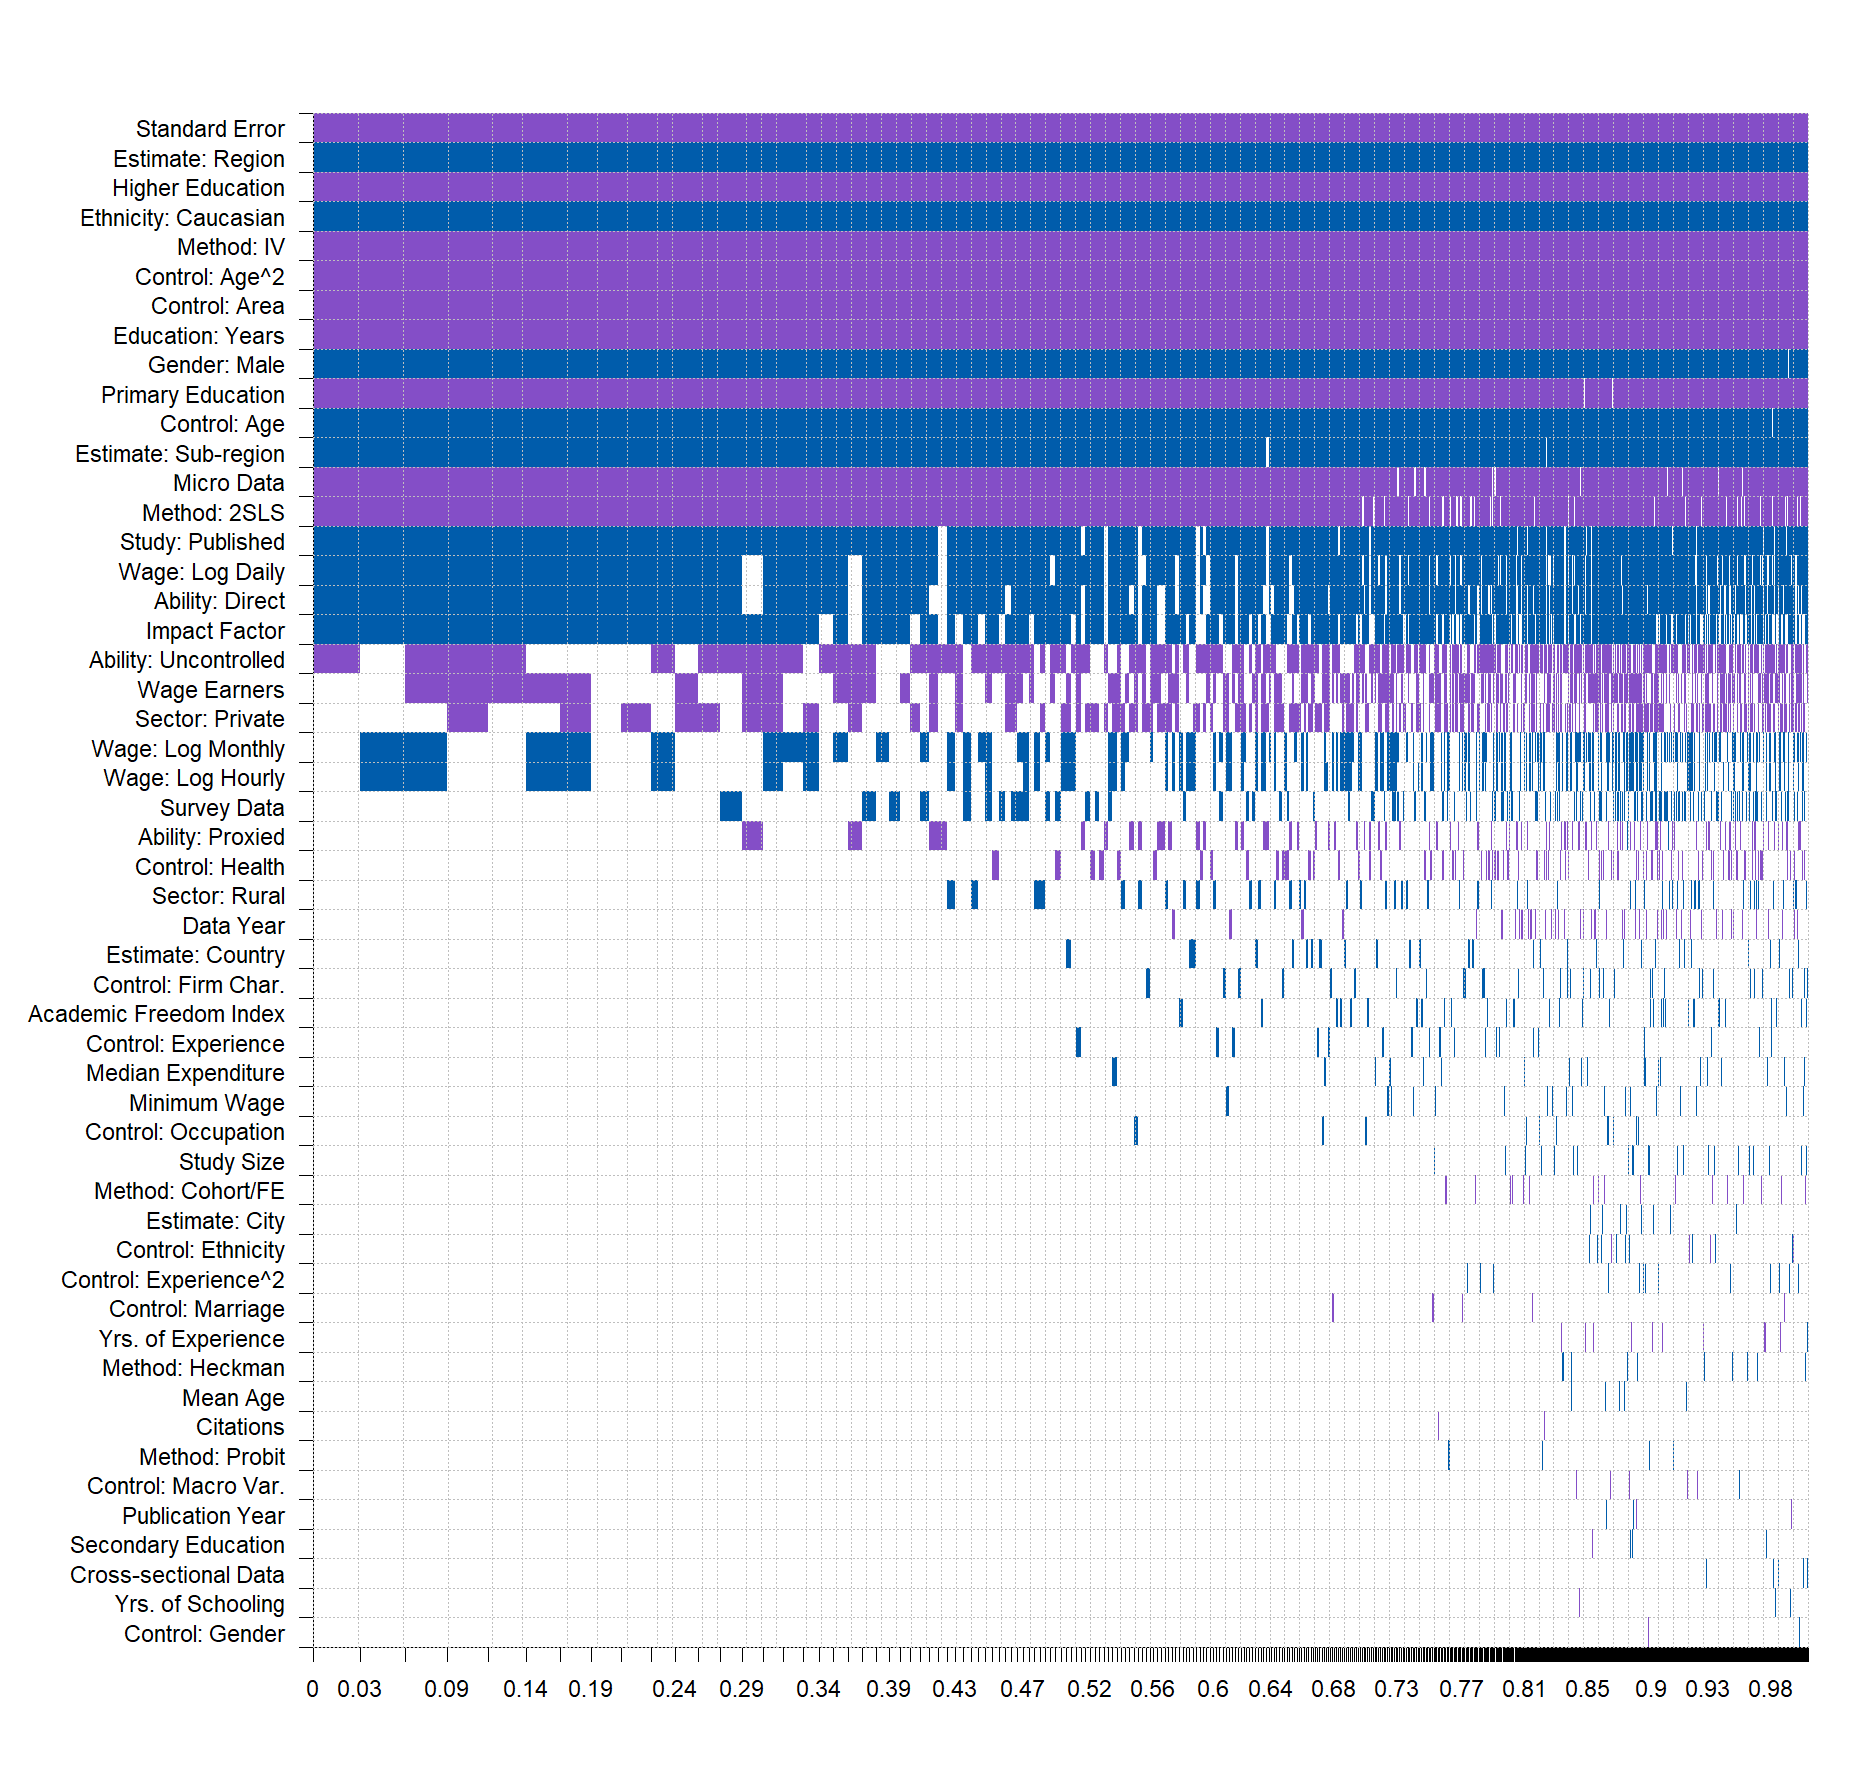
\includegraphics[width=1\textwidth]{Figures/bma_UIP_dilut_results.png}
\end{center}\vspace{-0.5cm}
\captionsetup{width=0.95\textwidth, font = scriptsize}
\caption*{\emph{Note:} This figure shows the results of the Bayesian model averaging using the uniform g-prior and dilution prior. The response variable, percentage returns to a year of schooling, is measured on the horizontal axis as cumulative posterior model probabilities. The explanatory variables are ranked in descending order on the vertical axis according to their posterior inclusion probability. Purple color: the variable is included in the model and has a positive sign. Blue color: the variable is included in the model and has a negative sign. Numerical results of the estimation can be found in table \ref{tab:BMA}. For a detailed explanation of the variables, see table \ref{tab:var}.
}
\end{figure}

As an additional robustness check, I also include \ac{FMA} with Mallow's criteria for weights \citep{hansen2007least} and orthogonalization of the model space as per \cite{amini2012comparison}. The reasons for this include higher resiliency against model misspecification or the reduction of model uncertainty. In other words, \ac{FMA} provides a good sanity check that the \ac{BMA} setup is not misspecified or overly complex.

I first present graphical results in \autoref{fig:BMA}. Each variable's contribution is marked by one of two colors - purple means a positive influence on the effect, while blue represents a negative influence. The columns in the figure each represent a single regression model, while the rows display the inclusion of variables in these models. The left-hand side of the figure shows the best models that best fit the data. The width of each column then captures the individual model's \ac{PMP}. The proportion of models a variable is included in gives that variable's \ac{PIP}. For example, if it is included in 50\% of models, its \ac{PIP} will be 0.5. Based on the paper by \cite{kass1995bayes}, simple guidelines indicate that \ac{PIP} values between 0.5 and 0.75 suggest a weak influence on the effect, 0.75-0.9 indicate solid importance of the variable, values over 0.9 and below 0.99 mean strong influence and values over 0.99 are decisive in telling this variable is essential for explaining the effect's behavior. Even glancing into the figure, it is evident that over 15 variables have a \ac{PIP} over 0.5 in the averaging process. Looking at the fittest model, 19 variables out of 52 are included.

Next, I compare the results for both \ac{BMA} and \ac{FMA}, this time quantitatively using numeric coefficients associated with the variables. These are displayed in \autoref{tab:BMA}, where variables with \ac{PIP} over 0.5 in the \ac{BMA} have this statistic highlighted. There are 20 variables with \ac{PIP} over 0.5 in total. When it comes to \ac{FMA}, p-values of many variables are below 0.001, confirming that the models could identify a large amount of highly important effect drivers.

%BMA+FMA table

\afterpage{
\begin{singlespace}
\begin{notsotiny}
\begin{longtable}{
@{\hskip\tabcolsep\extracolsep\fill}
l
*{6}{c}
}
\caption{Model averaging results}  \label{tab:BMA}\\
\toprule
  \multicolumn{1}{l}{Response variable:} &   \multicolumn{3}{c}{Bayesian model averaging} & \multicolumn{3}{c}{Frequentist model averaging} \\
  \cmidrule(lr){2-4} \cmidrule(lr){5-7}
  \multicolumn{1}{l}{Returns to Year of Schooling} & Post. mean & Post. SD & PIP & Coef. & SE & p-value \\
\midrule
\endfirsthead
\caption[]{Model averaging results (continued)}\\
\toprule
  \multicolumn{1}{l}{Response variable:} &   \multicolumn{3}{c}{Bayesian model averaging} & \multicolumn{3}{c}{Frequentist model averaging} \\
  \cmidrule(lr){2-4} \cmidrule(lr){5-7}
  \multicolumn{1}{l}{Returns to Year of Schooling} & Post. mean & Post. SD & PIP & Coef. & SE & p-value \\
\midrule
\endhead
\bottomrule
\multicolumn{7}{r}{{\scriptsize Continued on next page}} \\
\endfoot
\endlastfoot

    Constant & -1.361 & NaN & \textbf{1.000} & 4.580 & 352.079 & 0.990 \\
    Standard Error & 0.378 & 0.065 & \textbf{1.000} & 0.515 & 0.197 & 0.009 \\
    \midrule

\multicolumn{7}{l}{\emph{Estimate characteristics}}\\	
    Estimate: City & -0.002 & 0.051 & 0.004 & 0.000 & 1.103 & 0.000 \\
    Estimate: Sub-region & -1.434 & 0.366 & \textbf{0.994} & -0.575 & 1.711 & 0.737 \\
    Estimate: Region & -1.328 & 0.262 & \textbf{1.000} & -0.695 & 1.292 & 0.591 \\
    Estimate: Country & -0.020 & 0.121 & 0.037 & 0.000 & 0.905 & 0.000 \\
     \midrule
    
\multicolumn{7}{l}{\emph{Data characteristics}}\\	
    Study Size & -0.002 & 0.027 & 0.011 & 0.000 & 0.371 & 0.000 \\
    Yrs. of Schooling & 0.000 & 0.003 & 0.004 & 0.000 & 0.002 & 0.000 \\
    Yrs. of Experience & 0.000 & 0.001 & 0.003 & 0.000 & 0.015 & 0.000 \\
    Education: Years & 1.175 & 0.225 & \textbf{1.000} & 1.354 & 0.630 & 0.032 \\
    Wage: Log Hourly & -0.270 & 0.421 & 0.323 & 0.000 & 0.716 & 0.000 \\
    Wage: Log Daily & -1.403 & 0.689 & \textbf{0.900} & -0.465 & 1.242 & 0.708 \\
    Wage: Log Monthly & -0.443 & 0.591 & 0.408 & 0.000 & 1.016 & 0.000 \\
    Micro Data & 1.383 & 0.313 & \textbf{0.993} & 0.703 & 0.790 & 0.374 \\
    Survey Data & -0.091 & 0.233 & 0.160 & 0.000 & 0.583 & 0.000 \\
    Cross-sectional Data & -0.001 & 0.016 & 0.004 & 0.000 & 0.117 & 0.000 \\
    Data Year & 0.705 & 5.380 & 0.023 & 0.000 & 46.698 & 0.000 \\
    \midrule
    
\multicolumn{7}{l}{\emph{Spatial/structural variation}}\\
    Primary Education & 3.561 & 0.836 & \textbf{0.999} & 2.112 & 1.995 & 0.290 \\
    Secondary Education & 0.001 & 0.051 & 0.002 & 0.000 & 0.372 & 0.000 \\
    Higher Education & 5.543 & 0.596 & \textbf{1.000} & 4.391 & 1.450 & 0.002 \\
    Wage Earners & 0.691 & 0.790 & 0.486 & 0.000 & 1.410 & 0.000 \\
    Gender: Male & -1.212 & 0.279 & \textbf{1.000} & -0.757 & 0.708 & 0.285 \\
    Sector: Private & 0.721 & 0.937 & 0.419 & 0.000 & 2.079 & 0.000 \\
    Ethnicity: Caucasian & -1.455 & 0.269 & \textbf{1.000} & -1.083 & 0.540 & 0.045 \\
    Sector: Rural & -0.077 & 0.319 & 0.066 & 0.000 & 1.264 & 0.000 \\
    Median Expenditure & -0.002 & 0.020 & 0.015 & 0.000 & 0.161 & 0.000 \\
    Minimum Wage & -0.002 & 0.017 & 0.014 & 0.000 & 0.009 & 0.000 \\
    Academic Freedom Index & -0.014 & 0.116 & 0.021 & 0.000 & 0.102 & 0.000 \\
    \midrule
    
\multicolumn{7}{l}{\emph{Estimation method}}\\   
    Mean Age & 0.000 & 0.017 & 0.001 & 0.000 & 0.087 & 0.000 \\
    Method: Cohort/FE & 0.001 & 0.034 & 0.004 & 0.000 & 0.242 & 0.000 \\
    Method: 2SLS & 1.481 & 0.461 & \textbf{0.976} & 0.467 & 1.079 & 0.665 \\
    Method: Heckman & -0.001 & 0.030 & 0.005 & 0.000 & 0.062 & 0.000 \\
    Method: Probit & 0.000 & 0.030 & 0.001 & 0.000 & 0.084 & 0.000 \\
    Method: IV & 2.632 & 0.356 & \textbf{1.000} & 1.691 & 0.881 & 0.055 \\
    Ability: Direct & -1.143 & 0.574 & \textbf{0.859} & -0.521 & 0.642 & 0.417 \\
    Ability: Proxied & 0.148 & 0.385 & 0.146 & 0.000 & 0.919 & 0.000 \\
    Ability: Uncontrolled & 0.554 & 0.481 & \textbf{0.685} & 0.000 & 0.947 & 0.000 \\
    Control: Age & -1.881 & 0.422 & \textbf{0.998} & -0.960 & 1.109 & 0.387 \\
    Control: Age$^2$ & 2.946 & 0.452 & \textbf{1.000} & 1.976 & 1.109 & 0.075 \\
    Control: Experience & -0.015 & 0.105 & 0.027 & 0.000 & 0.678 & 0.000 \\
    Control: Experience$^2$ & 0.000 & 0.013 & 0.002 & 0.000 & 0.182 & 0.000 \\
    Control: Ethnicity & 0.000 & 0.015 & 0.002 & 0.000 & 0.208 & 0.000 \\
    Control: Health & 0.051 & 0.194 & 0.079 & 0.000 & 0.591 & 0.000 \\
    Control: Gender & 0.000 & 0.012 & 0.003 & 0.000 & 0.237 & 0.000 \\
    Control: Marriage & 0.001 & 0.023 & 0.005 & 0.000 & 0.254 & 0.000 \\
    Control: Occupation & -0.007 & 0.067 & 0.015 & 0.000 & 0.003 & 0.000 \\
    Control: Firm Char. & -0.017 & 0.105 & 0.033 & 0.000 & 0.591 & 0.000 \\
    Control: Area & 1.781 & 0.235 & \textbf{1.000} & 0.927 & 1.004 & 0.356 \\
    Control: Macro Var. & 0.000 & 0.011 & 0.002 & 0.000 & 0.130 & 0.000 \\
    \midrule
    
\multicolumn{7}{l}{\emph{Publication characteristics}}\\   
    Impact Factor & -0.187 & 0.110 & \textbf{0.805} & -0.052 & 0.199 & 0.793 \\
    Citations & 0.000 & 0.005 & 0.005 & 0.000 & 0.111 & 0.000 \\
    Study: Published & -1.036 & 0.377 & \textbf{0.945} & -0.305 & 1.361 & 0.823 \\
    Publication Year & 0.000 & 0.017 & 0.003 & 0.000 & 0.042 & 0.000 \\
    \bottomrule
    \addlinespace[0.2em]
    

 \multicolumn{7}{>{\scriptsize}p{0.95\linewidth}}{\emph{Note:} This table presents the results of the Bayesian and Frequentist model averaging. Post. mean = Posterior Mean, Post. SD = Posterior Standard Deviation, PIP = Posterior Inclusion Probability, Coef. = Coefficient, SE = Standard Error, OLS = Ordinary Least Squares, FE = Fixed Effects, 2SLS = 2 Stage Least Squares. The variables with PIP > 0.5 are highlighted. For a detailed explanation of the variables, see table \ref{tab:var}.}
\end{longtable}
\end{notsotiny}
\end{singlespace}
}

Looking at these in more detail, the publication bias stands out immediately. Despite the mixed or otherwise lukewarm claims about its presence in \autoref{chap:four}, both presented models strongly suggest that publication bias appears in the data. The standard error coefficients are 0.378 and 0.515 for both respective models; both these coefficients are statistically significant. The \ac{PIP} of 1.000 associated with the coefficient in the \ac{BMA} model is the highest possible, and the p-value for the \ac{FMA} model is also below 0.01.

Let us now explore those variables that negatively influence the effect. Firstly, regional and sub-regional data appear to diminish the effect's magnitude, as does reporting the wage in daily units or having a male or Caucasian subject group. Furthermore, published studies are likewise associated with lower effect in both models, although the \ac{FMA} p-value tied to this claim does not hold enough significance. While the linear age coefficient pulls the effect heavily in the negative direction, the quadratic coefficient works in the opposite direction, ultimately contributing positively to the overall effect. Perhaps the most interesting out of the negative drivers, however, is the direct ability variable. Out of the other ability variables, it is associated with the highest \ac{PIP} and has the biggest influence on the effect. This potential evidence for ability bias is weakened only by the \ac{FMA} robustness check, where the p-value is not small enough to claim statistical significance.


Regarding variables that exert a positive influence on the effect as opposed to a negative one, two coefficients stand out the most. These are, first, primary education; second, higher education. Although the secondary education coefficient is insignificant for the \ac{BMA} model, this may further prove that education truly matters. Apart from this foreseeable conclusion, we can also see that data collected on the micro level positively influence the overall effect, as does estimating the equation using 2-stage least squares or an instrumental variable regression. Controlling for the type of area in which the subjects work also has a significant positive effect, as do the earlier mentioned age squared and standard error. Lastly, I would like to give attention to the \textit{Education: Years} variable, which also exhibits a significant positive impact on the effect. In line with \cite{churchill2018meta}, reporting the estimates in years rather than levels seems to be of systematic importance rather than a fluke. I can think of two sources of this phenomenon - the functional form of \autoref{eq:schooling_levels} and human error. While the former may be induced purely by imperfect modeling of the relationship between an attained level of education and the returns associated with each year spent studying for that level, the latter appears less streamlined. Given that all estimates reported in levels had to be transformed and unified using a calculation with incomplete information (sometimes the number of years necessary to finish a certain degree was missing), this uncertainty may give rise to the systematic influence we observe.

As the last piece of information added to the model averaging topic, I also present the differences between posterior inclusion probabilities of models ran under different specifications, namely different priors. Apart from the above-mentioned uniform g-prior and dilution model prior, I run the estimation for three unique pairs of priors. These are, listed in an arbitrary order, uniform g-prior \& uniform model prior, benchmark g-prior \& random model prior, and Hannah-Quin criterion g-prior \& random model prior. The posterior inclusion probabilities of variables ran under all these specifications are displayed in \autoref{fig:BMA_comparison}. The results appear highly stable and invariable towards different specifications, and I find no further need to dig deeper in this regard. For a graphical display of results under each of the three additional specifications, see \autoref{app:three}.

\begin{figure}[!t]
\begin{center}
\caption{Inclusion probability varies little across different model specifications}
\label{fig:BMA_comparison}
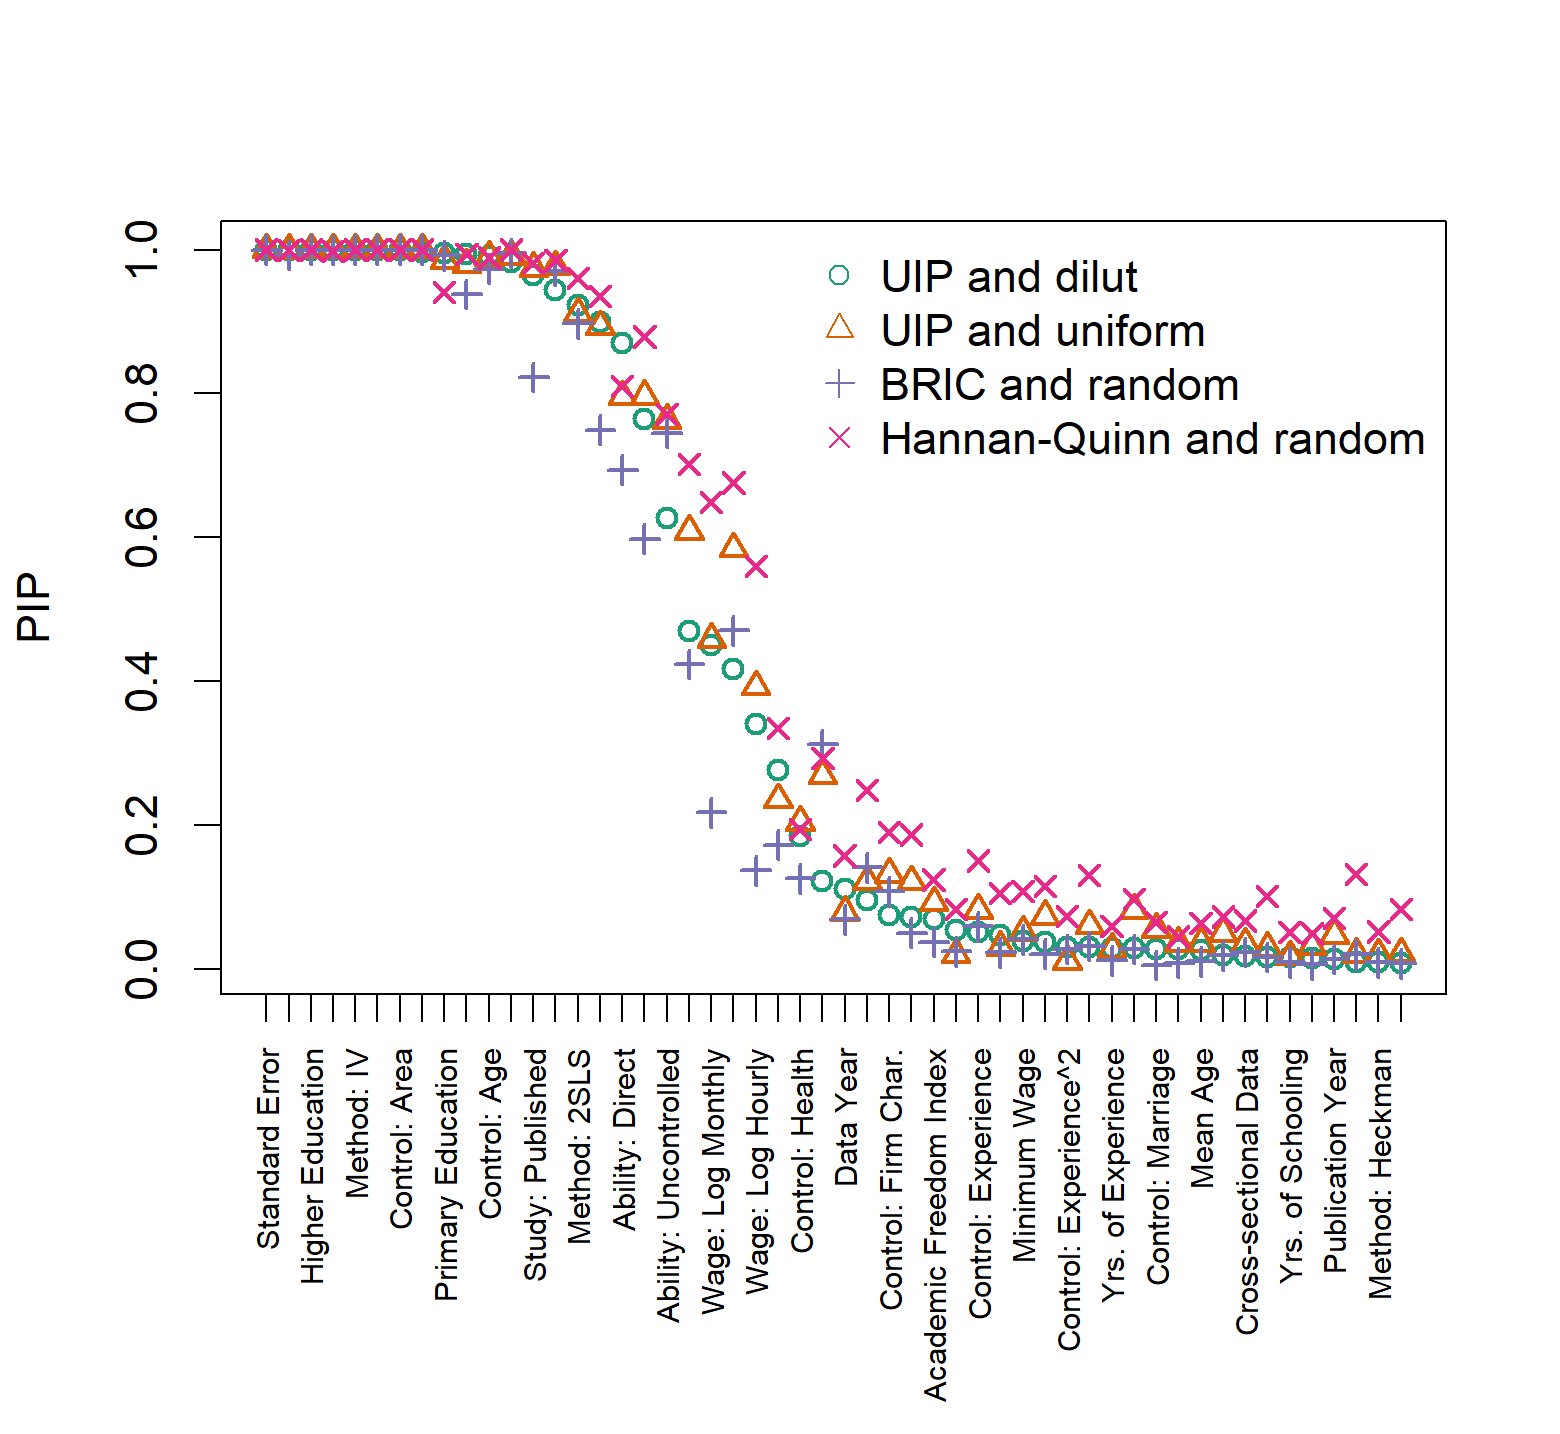
\includegraphics[width=0.8\textwidth]{Figures/bma_comparison.png}
\end{center}\vspace{-0.5cm}
\captionsetup{width=0.8\textwidth, font = scriptsize}
\caption*{\emph{Note:} This figure shows how much variables used in Bayesian model averaging contribute to the returns to education effect under different model specifications. The variables are displayed on the x-axis against their posterior inclusion probabilities on the y-axis. PIP = Posterior Inclusion Probability, UIP = Uniform g-prior, Dilut = Dilution Prior, Uniform = Uniform Model Prior, BRIC = Benchmark g-prior, Random = Random Model Prior, HQ = Hannan-Quinn Criterion. For the explanation of the variables and their detailed interpretation, see table \ref{tab:var}.}
\end{figure}

This concludes the chapter on model averaging. In \autoref{app:three}, you may find several robustness check figures, including the correlation table of utilized variables, graphical results, and a comparison of \ac{BMA} models ran under different specifications.


\chapter{The best-practice estimate}
\label{chap:six}
% grammar checked (07-26)

In this chapter, I would like to focus on one other method that can be used to gain more insight into the effect's behavior. The technique in question involves utilizing the \ac{BMA} model coefficients from \autoref{chap:five} and actual data values to obtain a best-practice estimate of the effect under different specifications. With this, I hope first to uncover more detail about how different experiment setups change the observed effect and second to bring even more insight into the question of individual variables and the magnitude of their influence on the effect.


\section{Modelling the best-practice}
\label{sec:best_practice_base}

With the \ac{BMA} model coefficients from \autoref{tab:BMA}, let us first model a baseline subjective practice by plugging in mostly arbitrary data values. Once this subjective best-practice is obtained, we can then compare it to individual setups of other studies. Regarding the values used for the subjective evaluation, I opt to keep most of them at their mean. It is unclear and, at times, impossible to objectively discern between one and another value of a variable and say which is better. There are, however, two notable exceptions. First, I set the standard error equal to zero, as publication bias is never desirable in the data sample. Second, I utilize the highest available values of the journal impact factor and number of citations available. This stems from the assumption that highly cited studies from top journals should bring more credibility and present estimates close to the true effect. 

Apart from this subjective best-practice estimate, I also computed best-practice estimates for all other studies in the dataset. When doing so, an important question arose of which specifications to use in case a study reported multiple estimates. When a variable remained constant for the study, such as for the number of citations or the impact factor, there was nothing to consider. However, if a variable changed from estimate to estimate, such as when each estimate was associated with a different method, I had to choose a representative value for the whole study. I opted to remedy this by using mode. In other words, I took the value that appeared the most often within the estimates of that study. A weighted mean of observations and their coefficients could have been used instead, but the loss of information incurred by the mode approach should be minimal. Given the large number of variables in the model, it should also not affect the overall picture.

\begin{table}[!htbp]
\centering
\scriptsize
\singlespace
\caption{Implied best-practice} 
\label{tab:BPE_base}
\begin{tabular}{
@{}
l
*{3}{c}
@{}}
\toprule
    Study & Estimate & 95\% Confidence Interval & Studies \\
\midrule
    Author & 6.536 & (5.762; 7.310)  & 0\\
    Query & 7.529 & (3.552; 11.506) & 74\\
    Snowballing & 6.346 & (2.530; 10.162) & 41\\
    All studies & 7.109 & (3.046; 11.17) & 115\\
\bottomrule
\multicolumn{4}{>{\scriptsize}p{0.6\linewidth}}{\emph{Note:} The table reports estimates of the best-practice estimate according to the author's subjective best-practice, two subsets of the literature, and the whole data sample. For the latter three, the figures are computed by averaging the best-practice estimates of all studies within that data subset. 95\% confidence interval bounds are constructed as an approximate using OLS with study level clustered standard errors. Query = Studies identified by query, Snowballing = Studies identified by snowballing, Studies = Number of studies used for the estimation.}
\end{tabular}
\end{table}

As a baseline, I present the results of the implied best-practice calculation using my subjective setup. Then, I display estimates calculated across different subsets of literature for studies identified separately by the query and by the snowballing. Furthermore, I construct an estimate using all studies in the dataset. These can all be found in \autoref{tab:BPE_base}. The subjective best-practice estimate equals 6.536\% with a relatively narrow confidence band. The estimates for the two literature subsets then fall within 1\% of the subjective estimate; the query literature predicts 7.529\% returns to schooling, while the snowballing literature suggests 6.346\%. Understandably, the confidence bounds for these two estimates are much wider, given the large number of studies used in the estimation, together with the fact that this lumps together studies of a much different nature. Still, one could argue that the query studies tend to report higher estimates than their snowballing counterpart, although this claim would lack the statistical significance backup. When looking at the whole dataset, the suggested estimate tallies up to 7.109\% with a confidence bound much too wide to hold any statistical power. Despite this, I believe this number should serve
, above all, as a good sanity check, and I think it does just that, given its proximity to the simple literature effect mean identified in \autoref{tab:sum}.

\section{Implied best-practice within subsets of literature}
\label{sec:best_practice_subsets}

To better understand how the implied best-practice behaves within the literature, I calculated how the estimates changed when observed for different data subsets. Using the same variable grouping logic described in \autoref{sec:best_practice_base}, I split the data into an array of subsets and present these in both numeric and graphical formats. I choose this approach over focusing on individual studies as I believe it holds more information, but I append the best-practice estimates for all 115 studies in \autoref{app:four} for completeness.

Before getting to the actual results, several points about the technical procedure should be addressed, starting with a point on how the subsetting is done. Different variable types call for a different approach. In my data, I treated these different data types as follows. For dummy variables, the subset consists of studies where that dummy is equal to 0. For variables defined as ratios, such as the ratio of urban vs. rural workers, the subsets include studies where a given variable is the highest out of all its alternatives. For example, suppose that after choosing the most frequent values of the urban vs. rural workers variable, the ratio comes up to 0.25 vs. 0.75 (urban vs. rural). In that case, such a study gets put into the 'rural workers' category, given that these comprise the majority of the sample. The same is true for variables with multiple alternatives, such as for the variable capturing the highest achieved education. Suppose further that the ratio is the same for all variables of the same group. In that case, the representative is chosen randomly, eliminating potentially any bias given a large enough number of studies in the subset. Consequently, results from a sample containing fewer studies should be viewed with caution. And lastly, one note on handling float-type variables. Here, I use the median as the split point and divide the dataset into studies whose representative estimate is above and below this point.

Another important caveat that this approach brings with it lies in using the most frequent value as the representative value for each study. Naturally, this procedure leads to a loss of information, skewing the overall statistics a bit as a result. For example, the number of citations median of the grouped sample of studies is no longer 80 as in the ungrouped dataset, but 73. As I mentioned in \autoref{sec:best_practice_base}, this could be remedied by weighting each variable with the number of occurrences within the reported estimates of each study. Personally, however, I consider the overall impact of this shortcoming minimal. Moreover, it could be argued that the best practice in literature is the one that each study tends to employ the most, but that, too, is up for debate.

As a last technical point regarding the results, I choose to omit several data subsets from the analysis for presentation clarity. With the formidable number of estimates presented, I firmly believe the shown results accurately represent the overall behavior within the literature and that they paint a clear enough picture. The numeric results can be found in \autoref{tab:bpe_summary_stats}, while the graphs appear in \autoref{fig:bpe_graphs}.


% BPE summary statistics
% \begin{table}[!htbp]
% \centering
% \scriptsize
% \singlespace
% \caption{Implied best-practice across various subsets of data}
% \label{tab:bpe_summary_stats}
% \begin{tabular}{
% @{}
% l % Description
% *{7}{c} % Middle columns
% >{\centering\arraybackslash}p{1cm} % Last column with fixed width
% @{}
% }
% \toprule
%     & Mean & \multicolumn{2}{c}{95\% conf. int.} & Median & Min & Max & SD & Studies \\
  
% \midrule

%                            All studies & 7.109 & 3.046   & 11.172  & 7.239 & 1.152 & 12.436 & 2.073 & 115 \\
%     \midrule
    
% \multicolumn{8}{l}{\emph{Data characteristics}}\\	
%      Yrs. of Schooling >= 10.6 & 6.907     & 3.199   & 10.615  & 6.749 & 3.503 & 11.598 & 1.892      & 59 \\
%       Yrs. of Schooling < 10.6 & 7.321     & 2.917   & 11.725  & 7.360 & 1.152 & 12.436 & 2.247      & 56 \\
%      Yrs. of Experience < 19.5 & 7.406     & 3.310   & 11.502  & 7.505 & 3.133 & 11.598 & 2.090      & 56 \\
%    Yrs. of Experience >= 19.45 & 6.826     & 2.837   & 10.815  & 6.790 & 1.152 & 12.436 & 2.035      & 59 \\
%               Education: Years & 7.119     & 3.181   & 11.057  & 7.134 & 1.152 & 12.436 & 2.009      & 84 \\
%              Education: Levels & 7.079     & 2.624   & 11.534  & 7.254 & 2.932 & 11.598 & 2.273      & 31 \\
%         National Register Data & 7.161     & 3.057   & 11.265  & 6.801 & 3.133 & 11.128 & 2.094      & 35 \\
%                     Micro Data & 7.484     & 4.313   & 10.655  & 7.573 & 4.168 & 11.146 & 1.618      & 18 \\
%                    Survey Data & 6.970     & 2.678   & 11.262  & 6.898 & 1.152 & 12.436 & 2.190      & 62 \\
%           Cross-sectional Data & 7.299     & 3.808   & 10.790  & 7.248 & 3.669 & 11.598 & 1.781      & 44 \\
%                     Panel Data & 6.991     & 2.601   & 11.381  & 6.979 & 1.152 & 12.436 & 2.240      & 71 \\
%               Higher Education & 7.729     & 3.380   & 12.078  & 7.463 & 3.745 & 11.598 & 2.219      & 23 \\
%            Secondary Education & 6.986     & 3.086   & 10.886  & 6.912 & 3.133 & 12.436 & 1.990      & 72 \\
%              Primary Education & 7.200     & 2.798   & 11.602  & 7.576 & 1.152 & 10.083 & 2.246      & 13 \\
%     \midrule
    
% \multicolumn{8}{l}{\emph{Spatial/structural variation}}\\
%                   No Education & 6.164     & 2.250   & 10.078  & 7.029 & 2.932  & 7.846 & 1.997       & 7 \\
%                   Wage Earners & 7.050     & 2.977   & 11.123  & 7.006 & 1.152 & 12.436 & 2.078     & 109 \\
%                  Self-Employed & 8.175     & 4.590   & 11.760  & 7.415 & 6.746 & 11.598 & 1.829       & 6 \\
%                   Gender: Male & 7.242     & 3.430   & 11.054  & 7.254 & 1.152 & 12.436 & 1.945      & 97 \\
%                 Gender: Female & 6.388     & 1.272   & 11.504  & 6.250 & 2.932 & 11.146 & 2.610      & 18 \\
%           Ethnicity: Caucasian & 6.907     & 3.650   & 10.164  & 6.749 & 4.015 & 11.146 & 1.662      & 31 \\
%               Ethnicity: Other & 7.183     & 2.851   & 11.515  & 7.360 & 1.152 & 12.436 & 2.210      & 84 \\
%                  Sector: Urban & 7.077     & 2.943   & 11.211  & 7.123 & 1.152 & 11.598 & 2.109     & 102 \\
%                  Sector: Rural & 7.353     & 3.782   & 10.924  & 7.256 & 5.191 & 12.436 & 1.822      & 13 \\
%                   Income: High & 7.192     & 3.684   & 10.700  & 6.912 & 3.745 & 11.261 & 1.790      & 60 \\
%                 Income: Middle & 7.077     & 2.414   & 11.740  & 7.368 & 1.152 & 12.436 & 2.379      & 48 \\
%                    Income: Low & 6.606     & 2.029   & 11.183  & 6.115 & 2.932 & 10.083 & 2.335       & 7 \\
%     Median Expenditure >= 8477 & 6.981     & 3.079   & 10.883  & 6.749 & 1.152 & 11.261 & 1.991      & 62 \\
%      Median Expenditure < 8477 & 7.258     & 2.993   & 11.523  & 7.319 & 3.133 & 12.436 & 2.176      & 53 \\
%             Minimum Wage < 345 & 6.976     & 2.860   & 11.092  & 7.282 & 1.152 & 12.436 & 2.100      & 57 \\
%            Minimum Wage >= 345 & 7.239     & 3.207   & 11.271  & 6.822 & 3.503 & 11.598 & 2.057      & 58 \\
%                 Mean Age >= 37 & 6.863     & 3.335   & 10.391  & 6.770 & 2.932 & 11.232 & 1.800      & 60 \\
%                  Mean Age < 37 & 7.377     & 2.824   & 11.930  & 7.402 & 1.152 & 12.436 & 2.323      & 55 \\
%                  \midrule

% \multicolumn{8}{l}{\emph{Estimation method}}\\  
%                    Method: OLS & 7.270     & 3.070   & 11.470  & 7.282 & 1.152 & 12.436 & 2.143      & 85 \\
%                   Method: 2SLS & 7.153     & 3.096   & 11.210  & 6.993 & 3.683 & 10.767 & 2.070       & 8 \\
%                Method: Heckman & 6.417     & 2.824   & 10.010  & 5.434 & 5.286  & 8.532 & 1.833       & 3 \\
%                     Method: IV & 6.774     & 3.223   & 10.325  & 7.029 & 4.015 & 10.424 & 1.812      & 11 \\
%              Method: Cohort/FE & 5.861     & 2.388    & 9.334  & 5.974 & 3.503  & 8.476 & 1.772       & 7 \\
%                 Method: Probit & 7.541        & NA       & NA  & 7.541 & 7.541  & 7.541    & NA       & 1 \\
%               Ability: Proxied & 6.729    & 2.531   & 10.927  & 7.006 & 2.932 & 11.232 & 2.142  &      23 \\
%           Ability: Unmentioned & 7.134    & 4.057   & 10.211  & 6.979 & 3.712 & 10.767 & 1.570  &      29 \\
%          Ability: Uncontrolled & 7.312    & 3.155   & 11.469  & 7.300 & 1.152 & 12.436 & 2.121  &      52 \\
%                Ability: Direct & 6.873    & 1.173   & 12.573  & 5.580 & 3.503 & 11.598 & 2.908  &      11 \\
%                    \midrule
    
% \multicolumn{8}{l}{\emph{Publication characteristics}}\\  
%         Impact Factor >= 0.222 & 7.066    & 3.270   & 10.862  & 6.890 & 3.503 & 12.436 & 1.937  &      58 \\
%          Impact Factor < 0.222 & 7.152    & 2.801   & 11.503  & 7.319 & 1.152 & 11.598 & 2.220  &      57 \\
%                Citations >= 73 & 7.130    & 3.453   & 10.807  & 7.134 & 3.656 & 11.261 & 1.876  &      58 \\
%                 Citations < 73 & 7.086    & 2.631   & 11.541  & 7.254 & 1.152 & 12.436 & 2.273  &      57 \\
%               Study: Published & 7.244    & 3.261   & 11.227  & 7.254 & 3.133 & 12.436 & 2.032  &      93 \\
%             Study: Unpublished & 6.535    & 2.227   & 10.843  & 6.749 & 1.152 & 11.146 & 2.198  &      22 \\

%     \bottomrule                                               
    
% \multicolumn{9}{>{\scriptsize}p{0.95\linewidth}}{\emph{Note:} This table displays implied best practice across the whole literature sample across different subsets of the main data. For determining the value of variables for each study, mode is used. For cutoff points of numeric, non-ratio type variables, medians are used. SD = Standard Deviation, OLS = Ordinary Least Squares, 2SLS = Two-stage Least Squares, IV = Instrumental Variable, FE = Fixed-Effects.}
% \end{tabular}
% \end{table}


% BPE graphs
%Education: years/levels
%Data type: panel/cross
%Highest achieved education
%Male vs female
%Income: high, low, middle
%Methods, 
%Ability, 
%Citations
\begin{figure}[!htbp]
\begin{center}
\caption{Implied best-practice across various subsets of data}
\label{fig:bpe_graphs}

\begin{subfigure}[!htbp]{0.38\textwidth}
   \vspace{-0.1cm}
   \caption{Education type}
   \vspace{-0.1cm}
   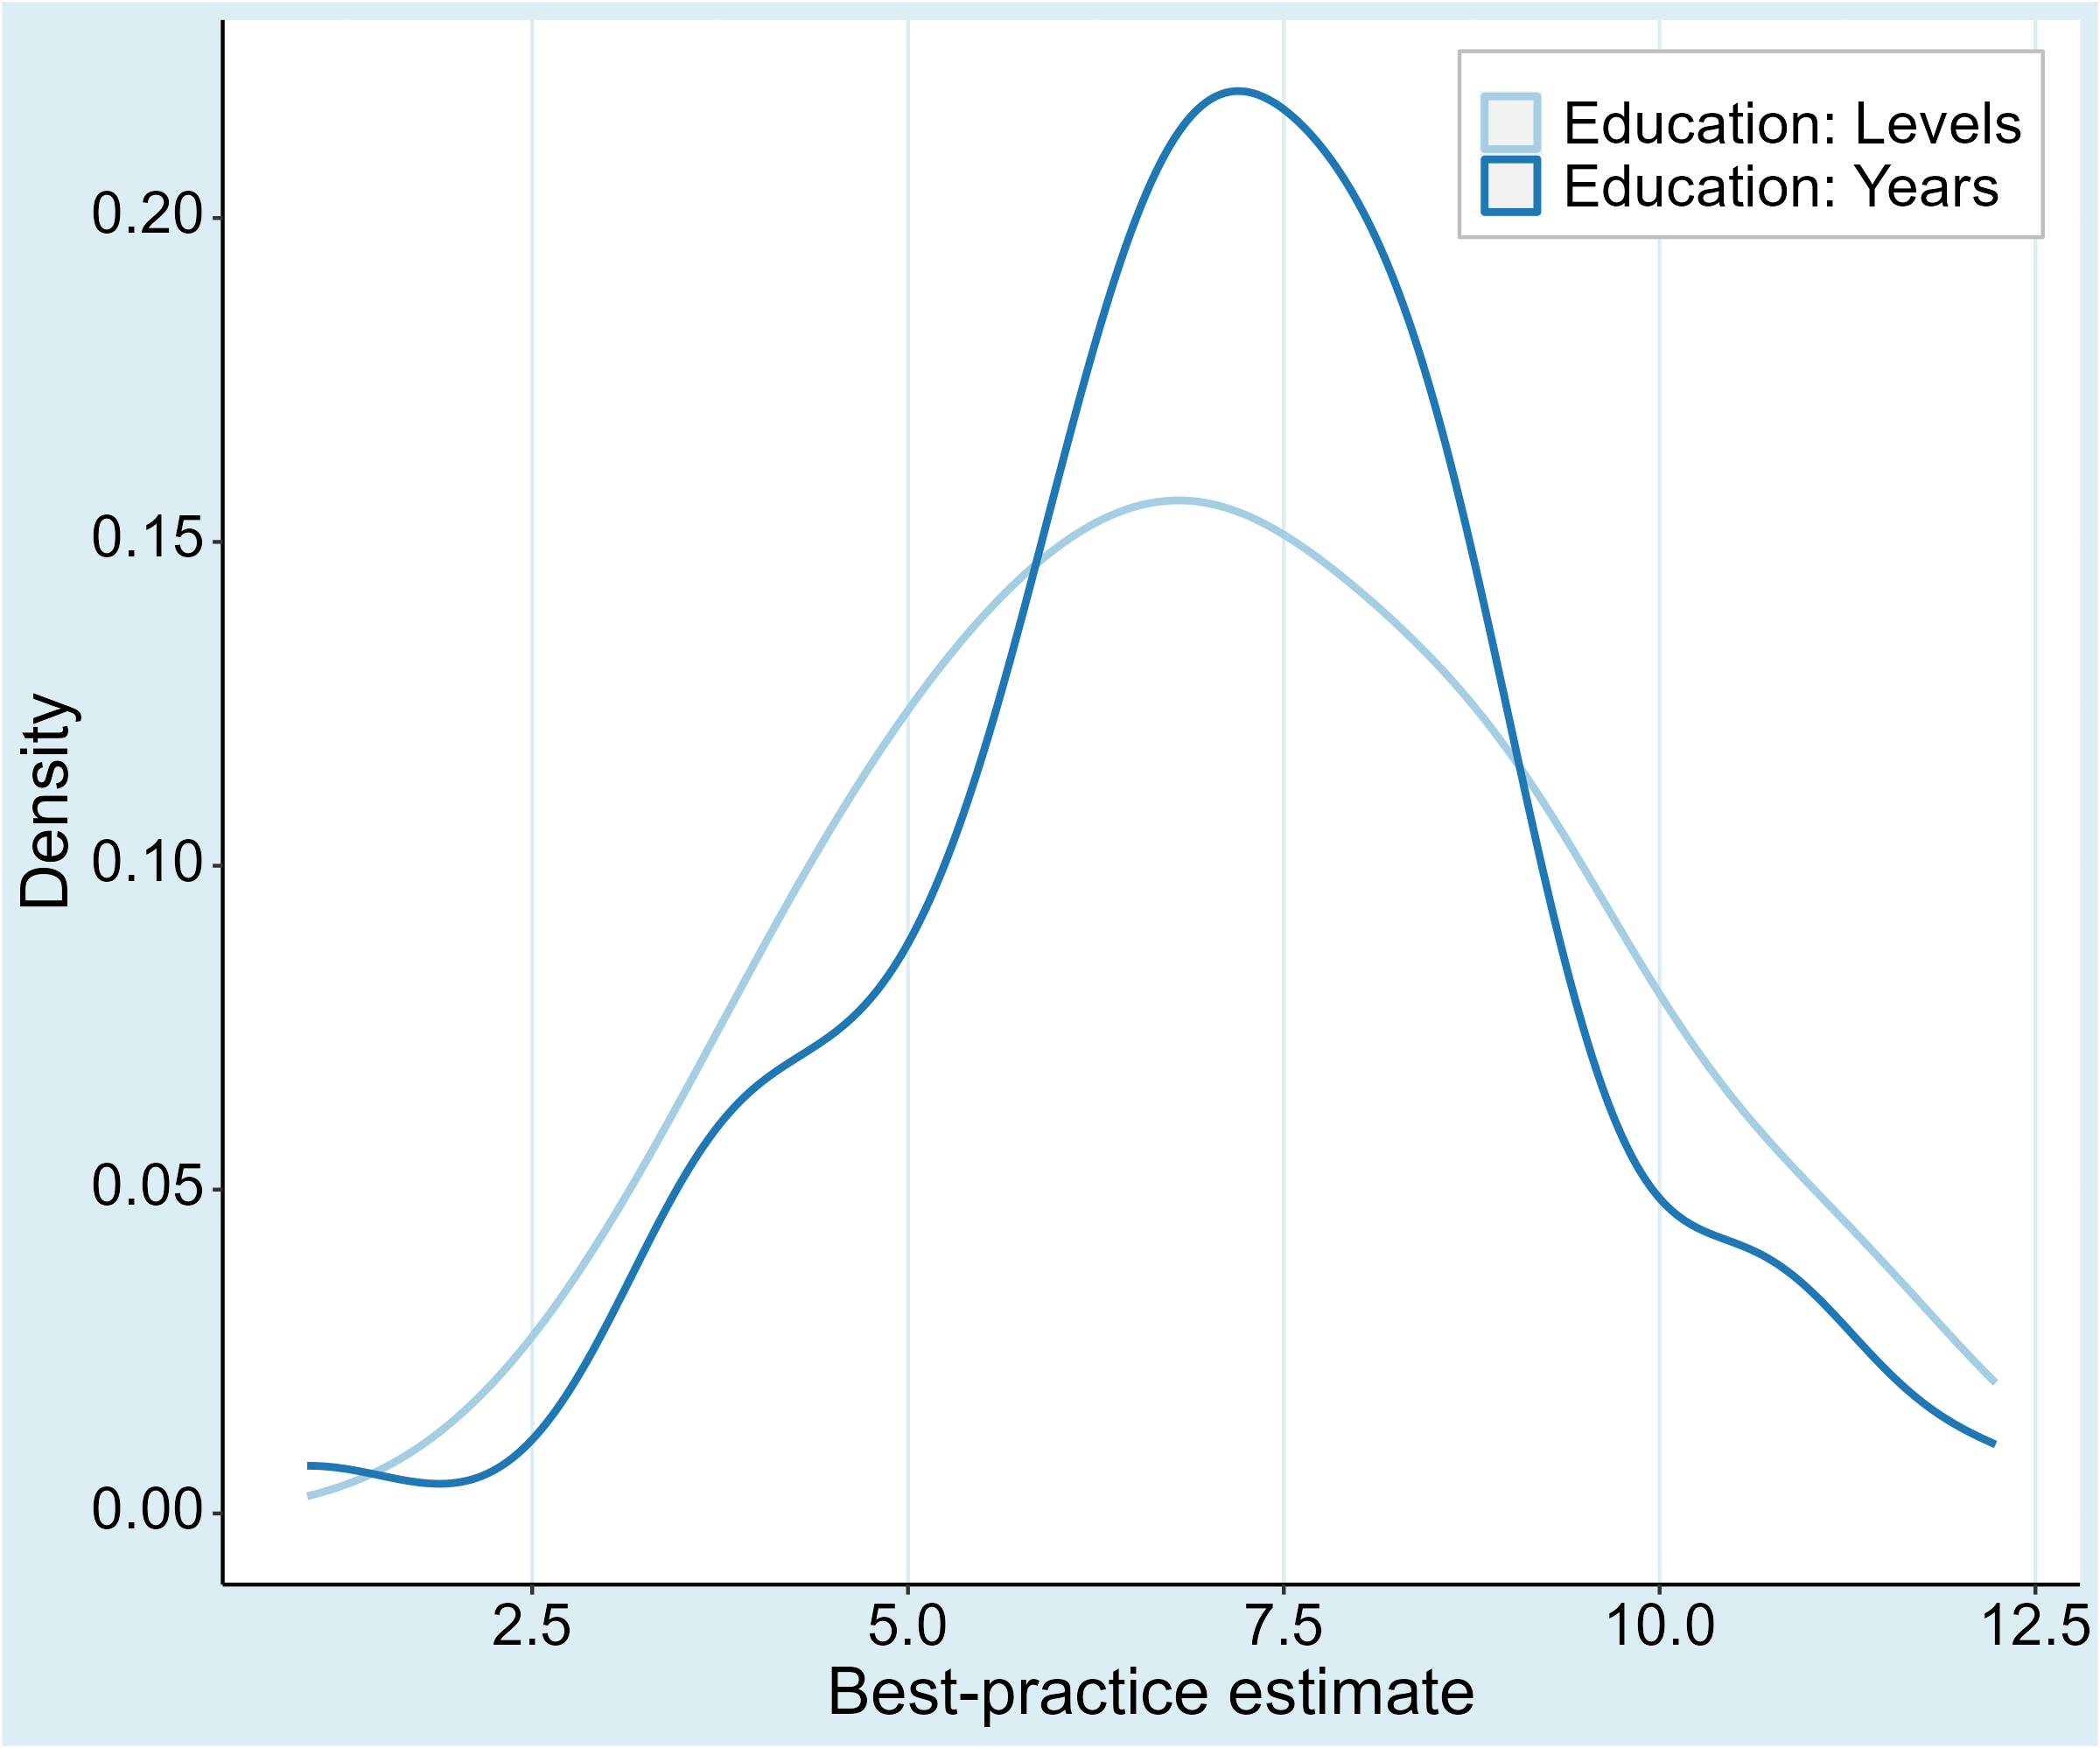
\includegraphics[width=0.95\linewidth]{Figures/BPE/bpe_years_levels.png}
   \label{fig:bpe_years_levels}
\end{subfigure}
\begin{subfigure}[!htbp]{0.38\textwidth}
   \vspace{-0.1cm}
   \caption{Data type}
   \vspace{-0.1cm}
   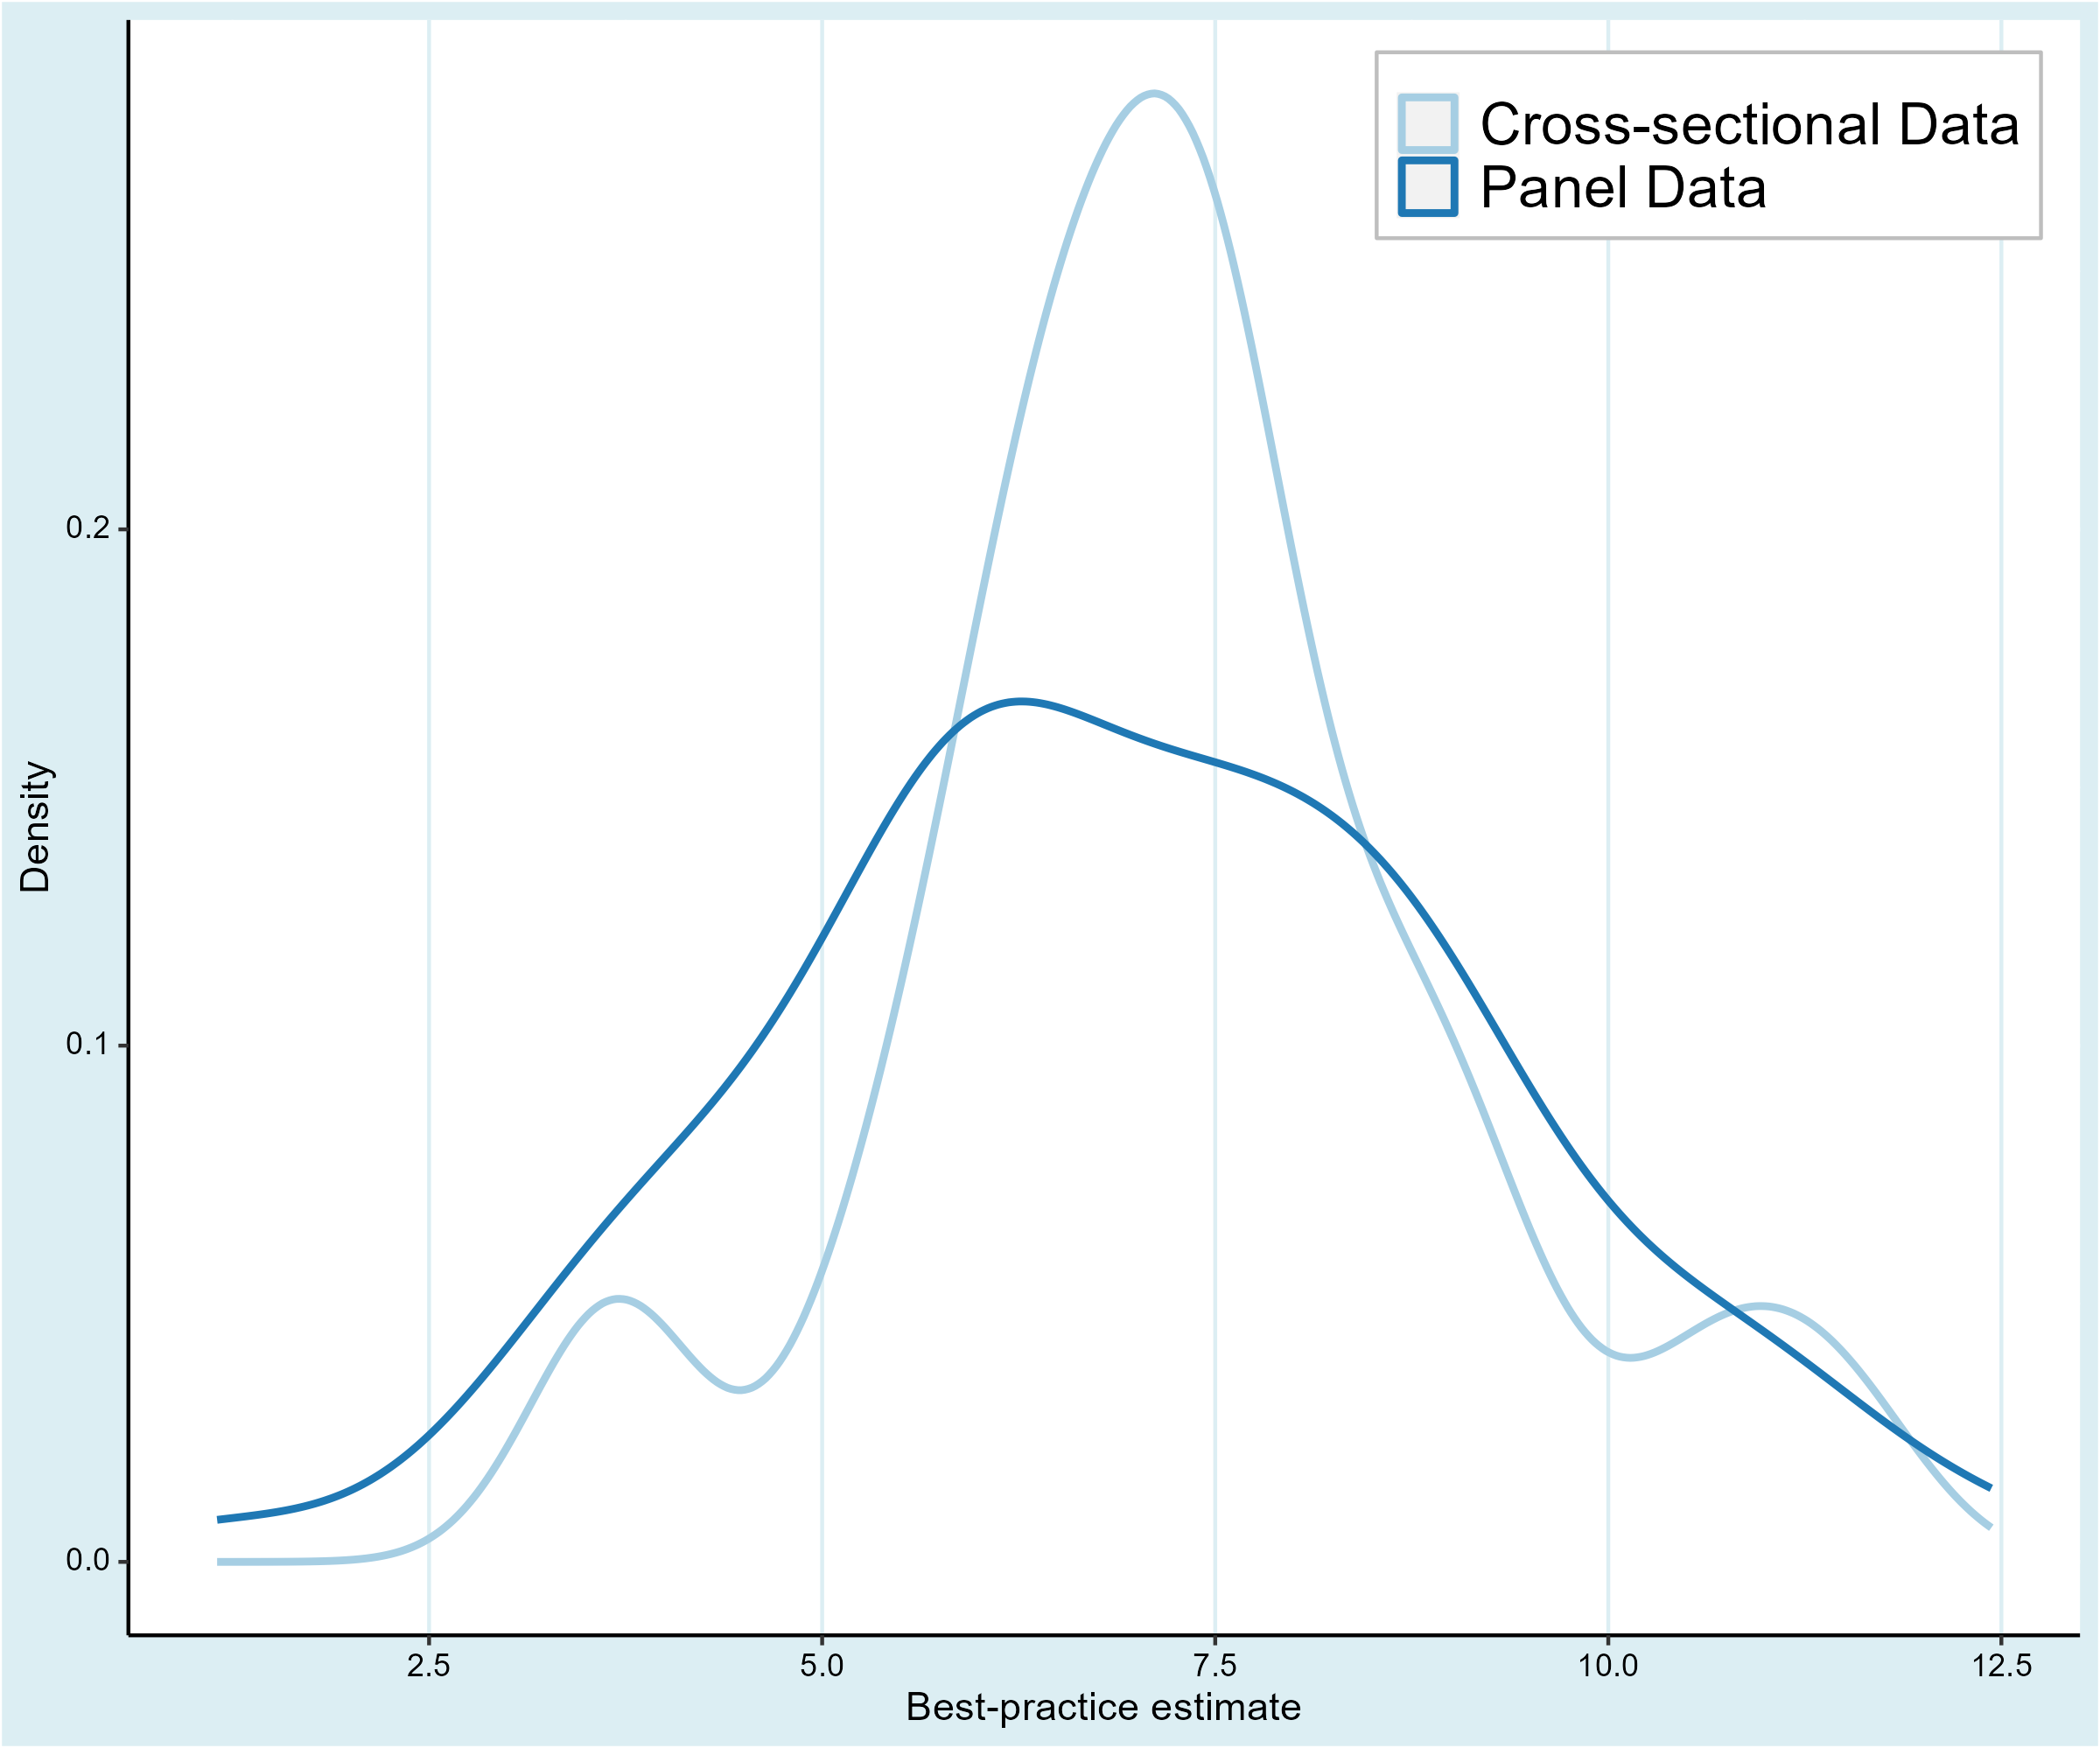
\includegraphics[width=0.95\linewidth]{Figures/BPE/bpe_data_type.png}
   \label{fig:bpe_data_type}
\end{subfigure}

\begin{subfigure}[!htbp]{0.38\textwidth}
   \vspace{0.2cm}
   \caption{Highest education}
   \vspace{-0.1cm}
   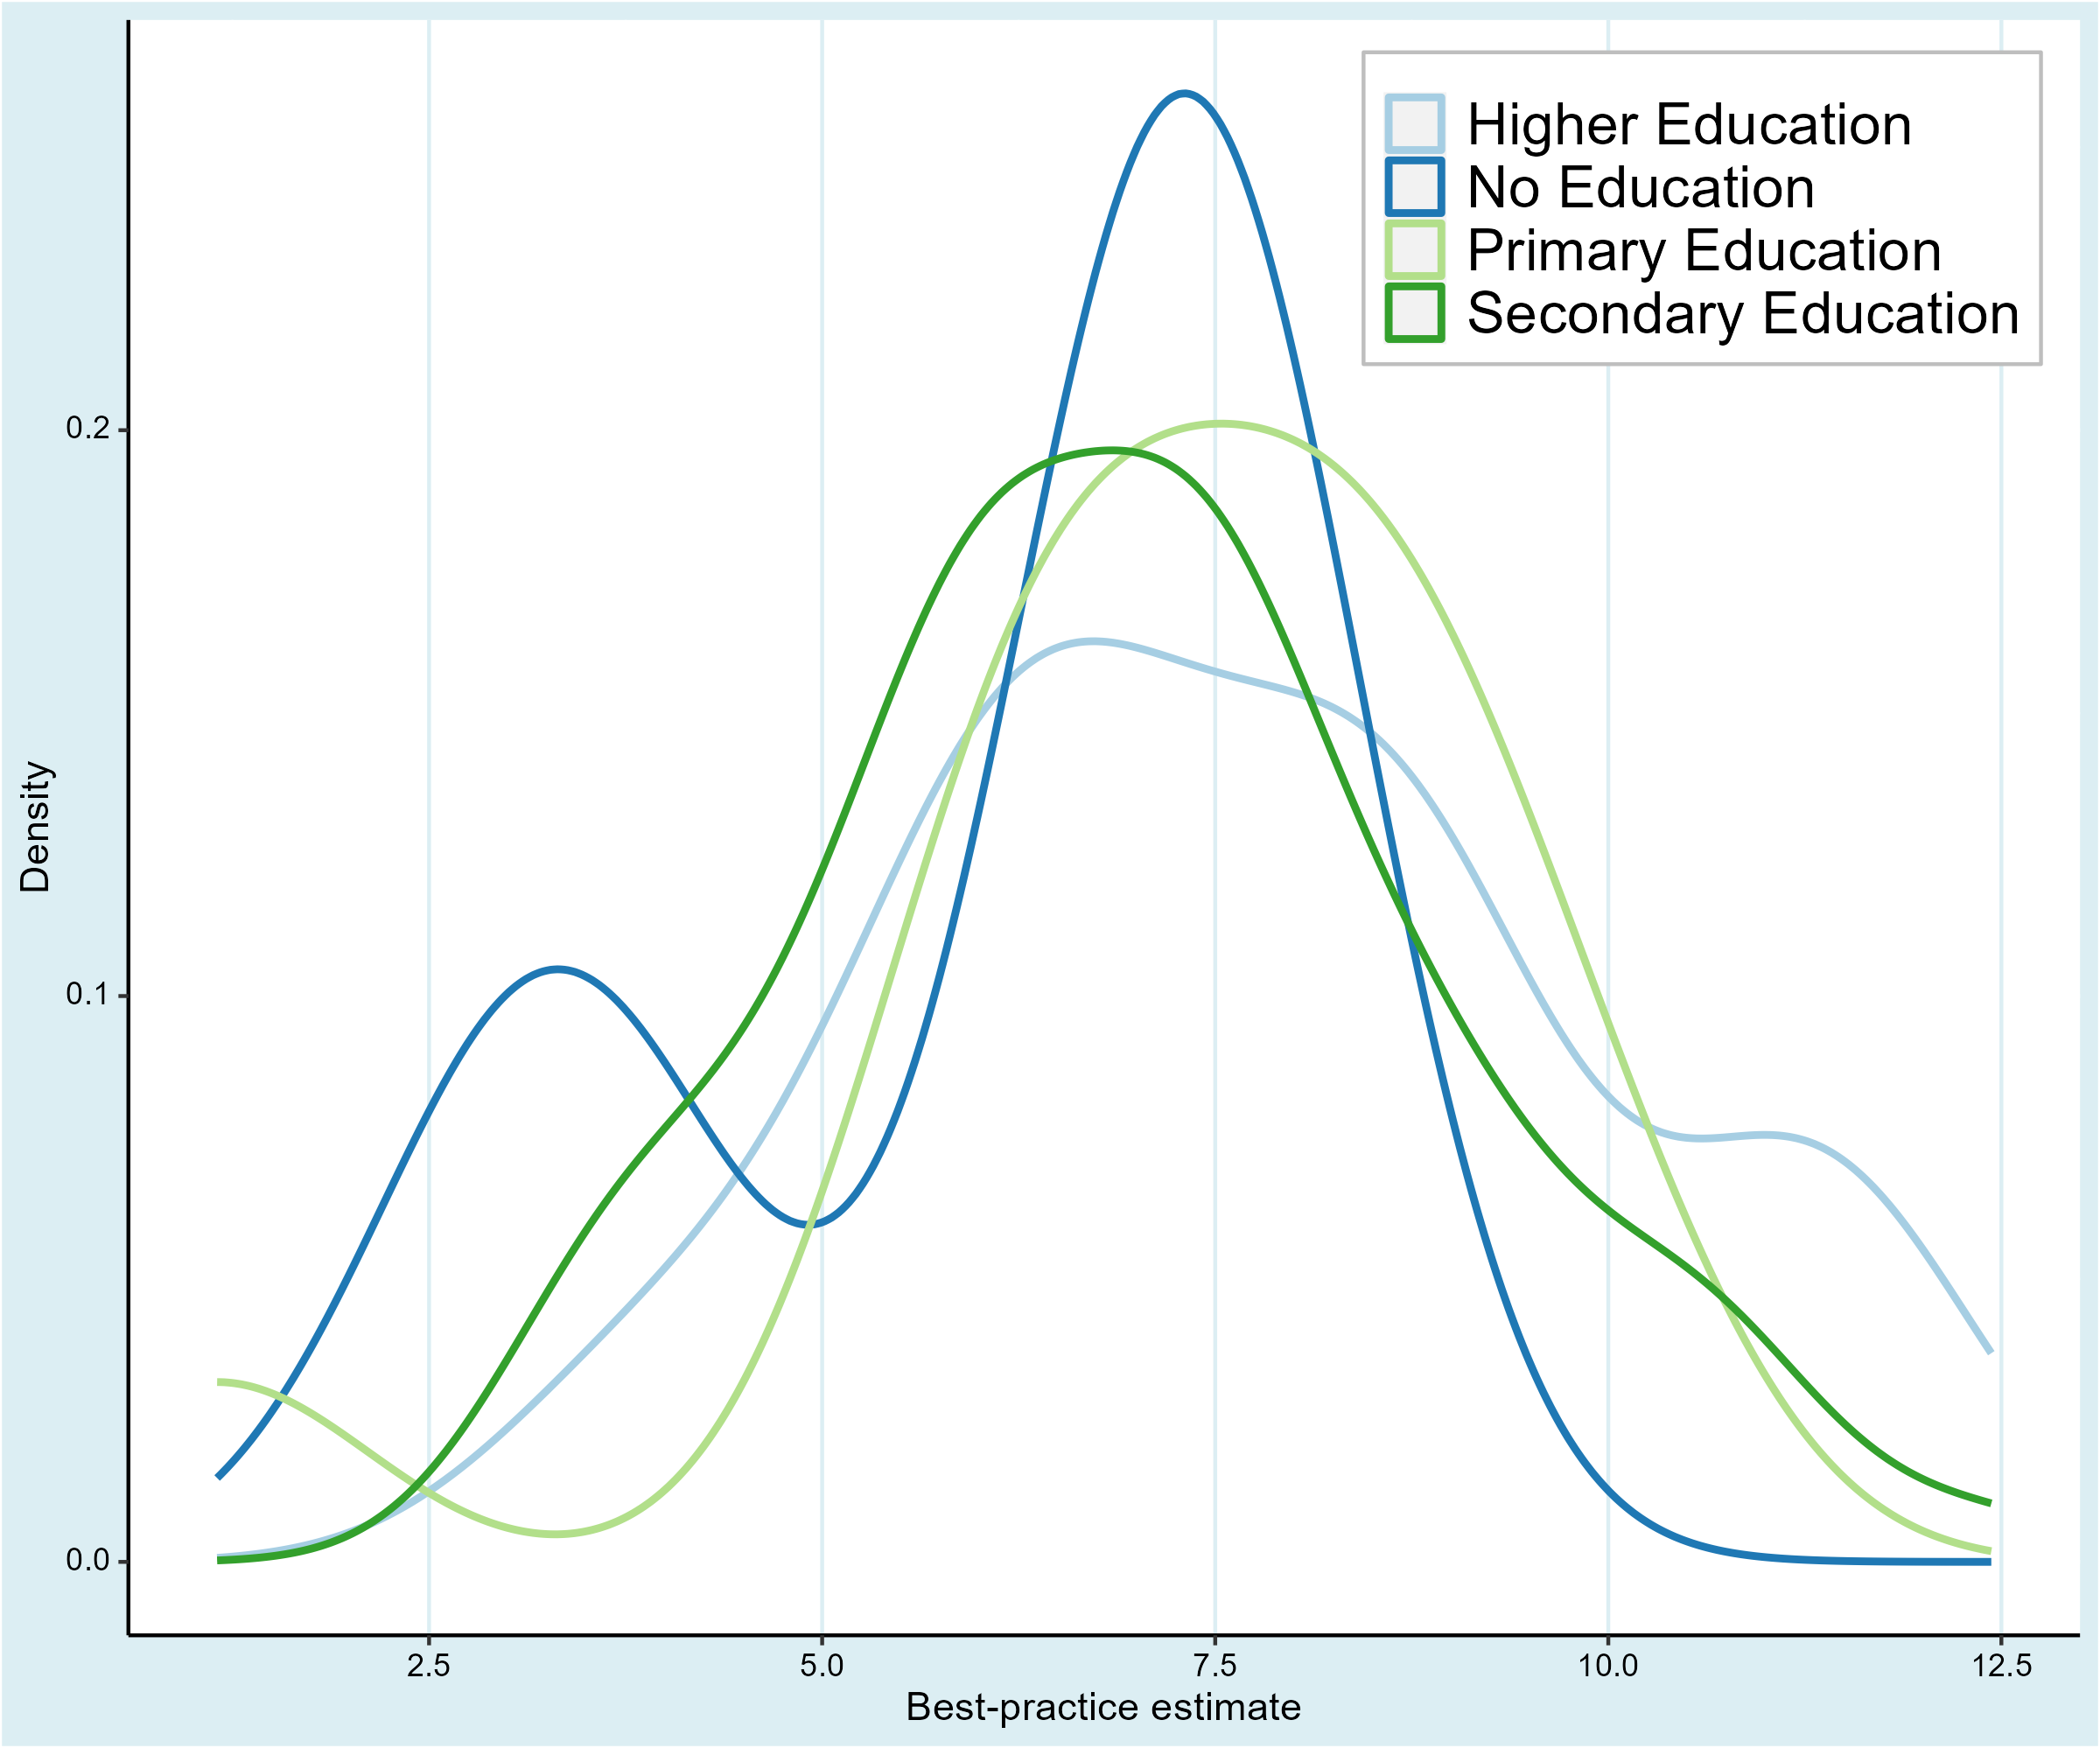
\includegraphics[width=0.95\linewidth]{Figures/BPE/bpe_education.png}
   \label{fig:bpe_education}
\end{subfigure}
\begin{subfigure}[!htbp]{0.38\textwidth}
   \vspace{0.2cm}
   \caption{Gender}
   \vspace{-0.1cm}
   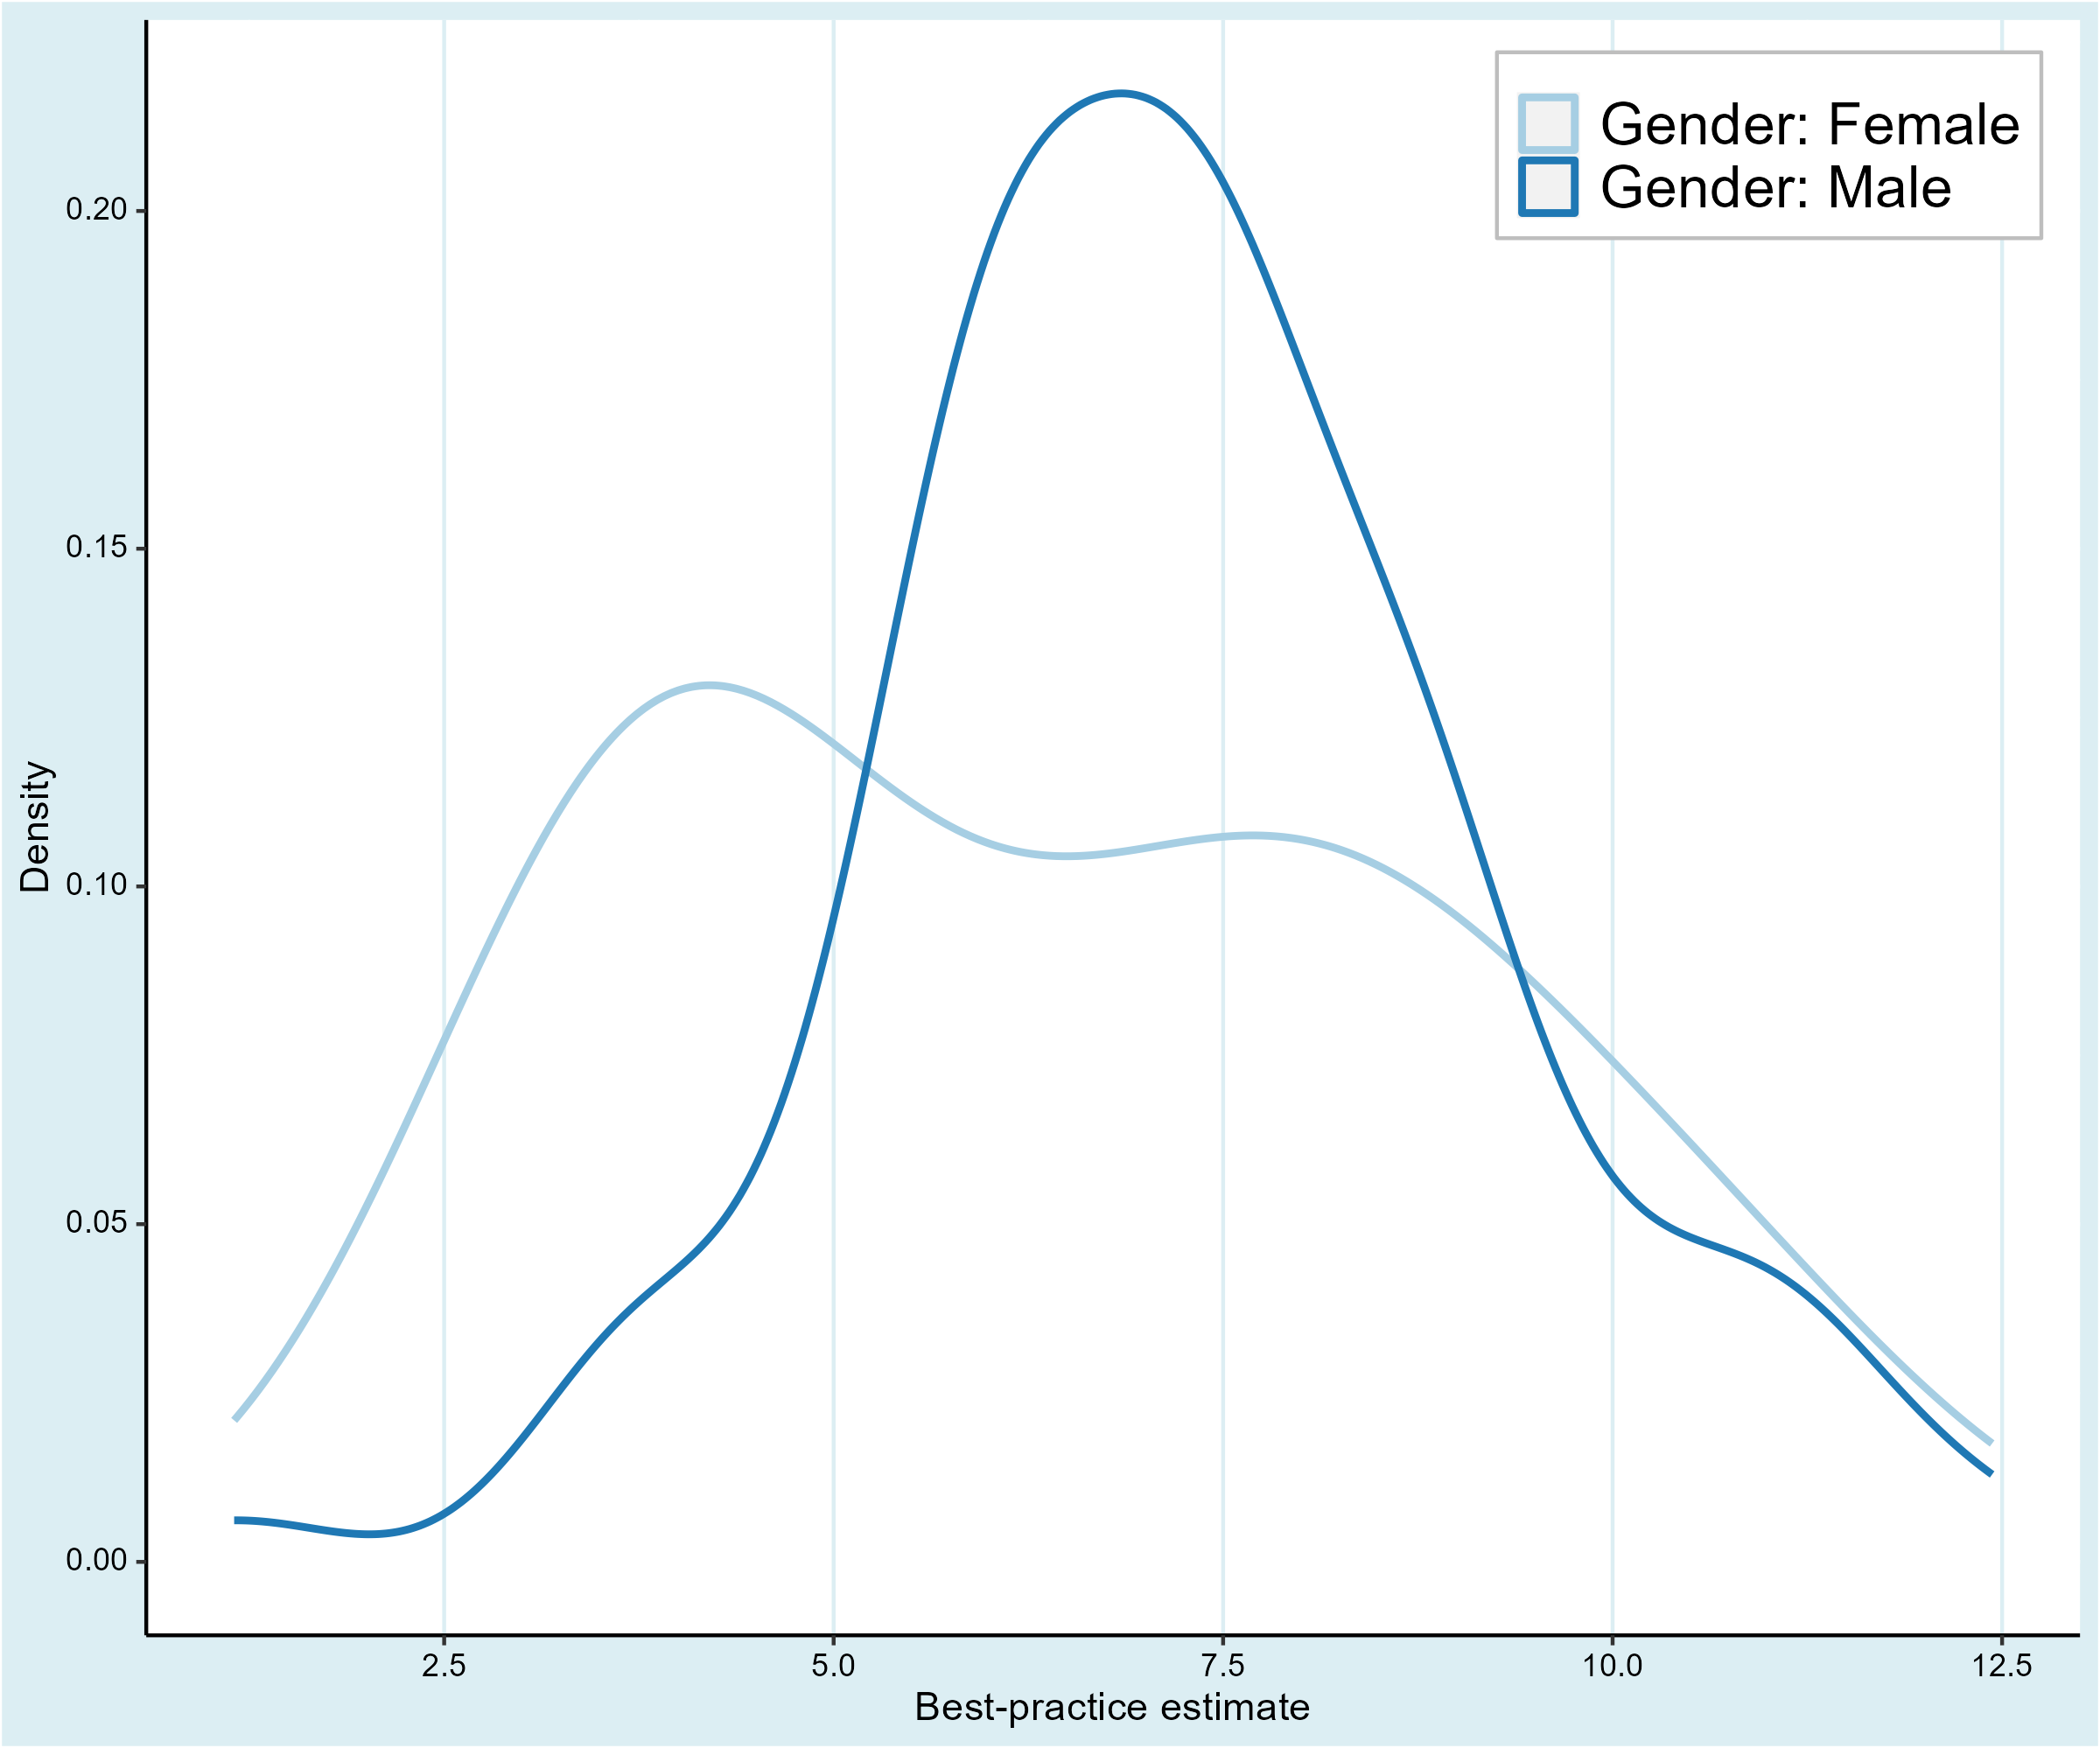
\includegraphics[width=0.95\linewidth]{Figures/BPE/bpe_gender.png}
   \label{fig:bpe_gender}
\end{subfigure}

\begin{subfigure}[!htbp]{0.38\textwidth}
   \vspace{0.2cm}
   \caption{Country wealth}
   \vspace{-0.1cm}
   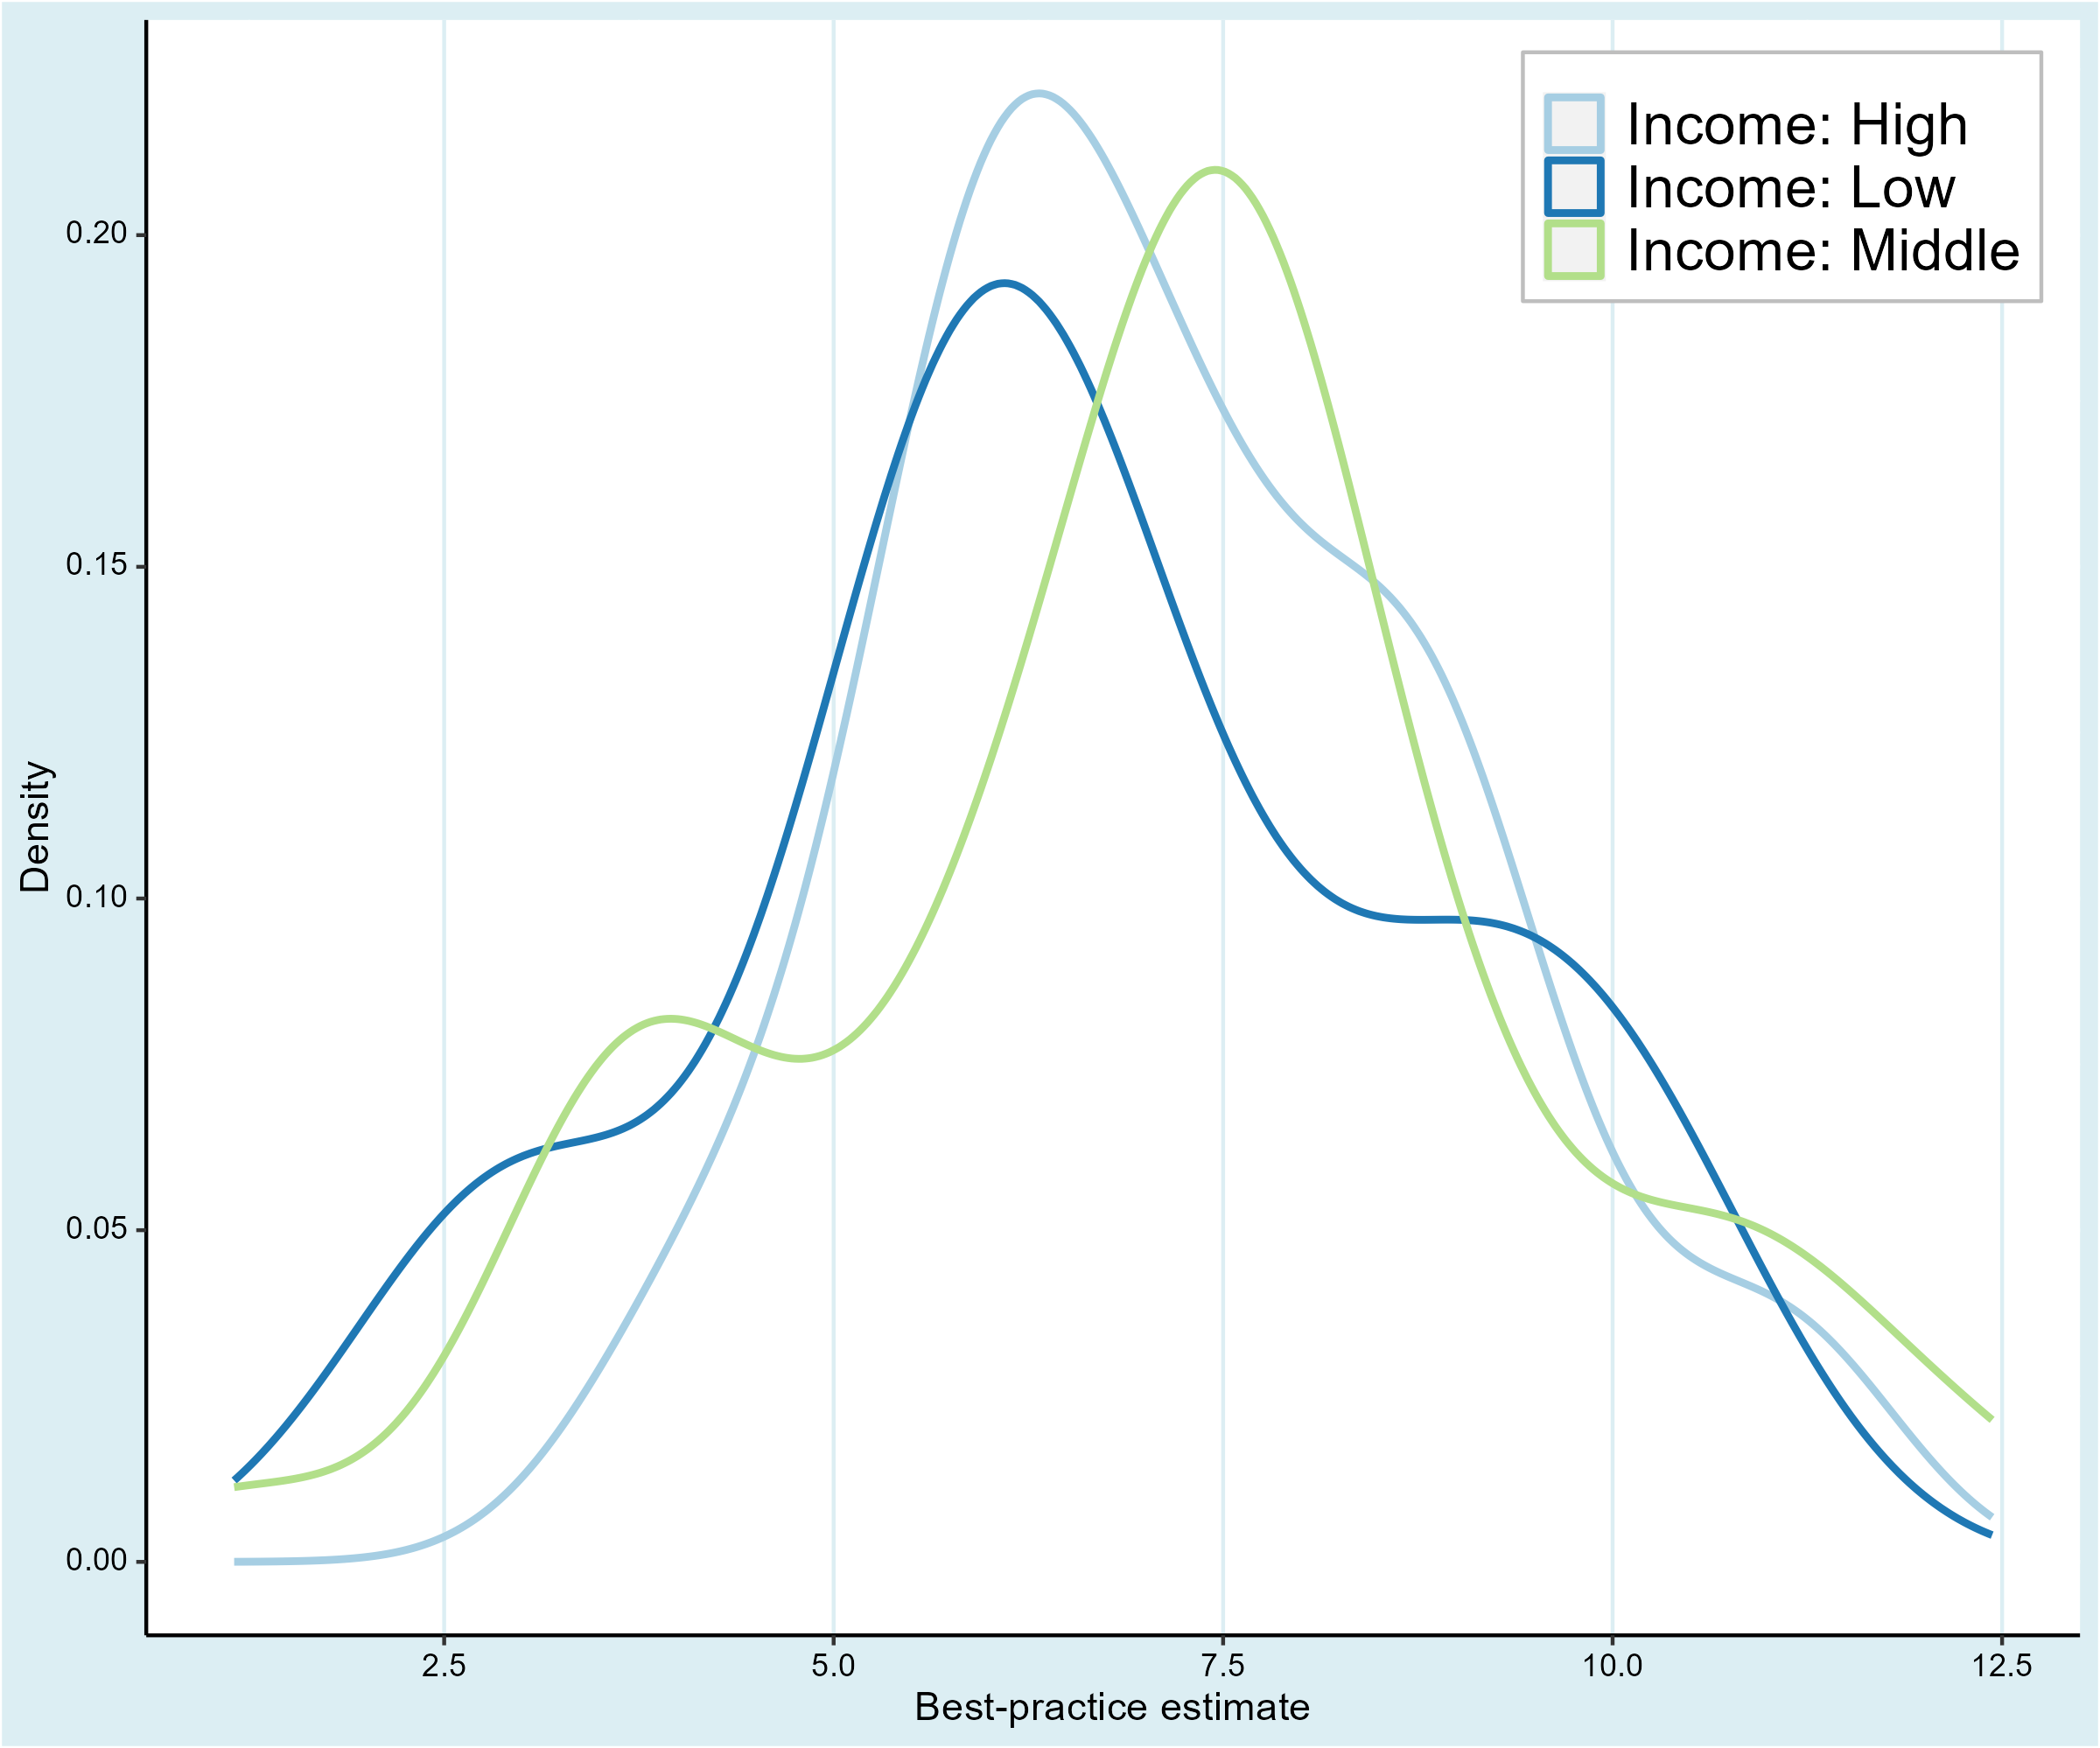
\includegraphics[width=0.95\linewidth]{Figures/BPE/bpe_income.png}
   \label{fig:bpe_income}
\end{subfigure}
\begin{subfigure}[!htbp]{0.38\textwidth}
   \vspace{0.2cm}
   \caption{Estimation method}
   \vspace{-0.1cm}
   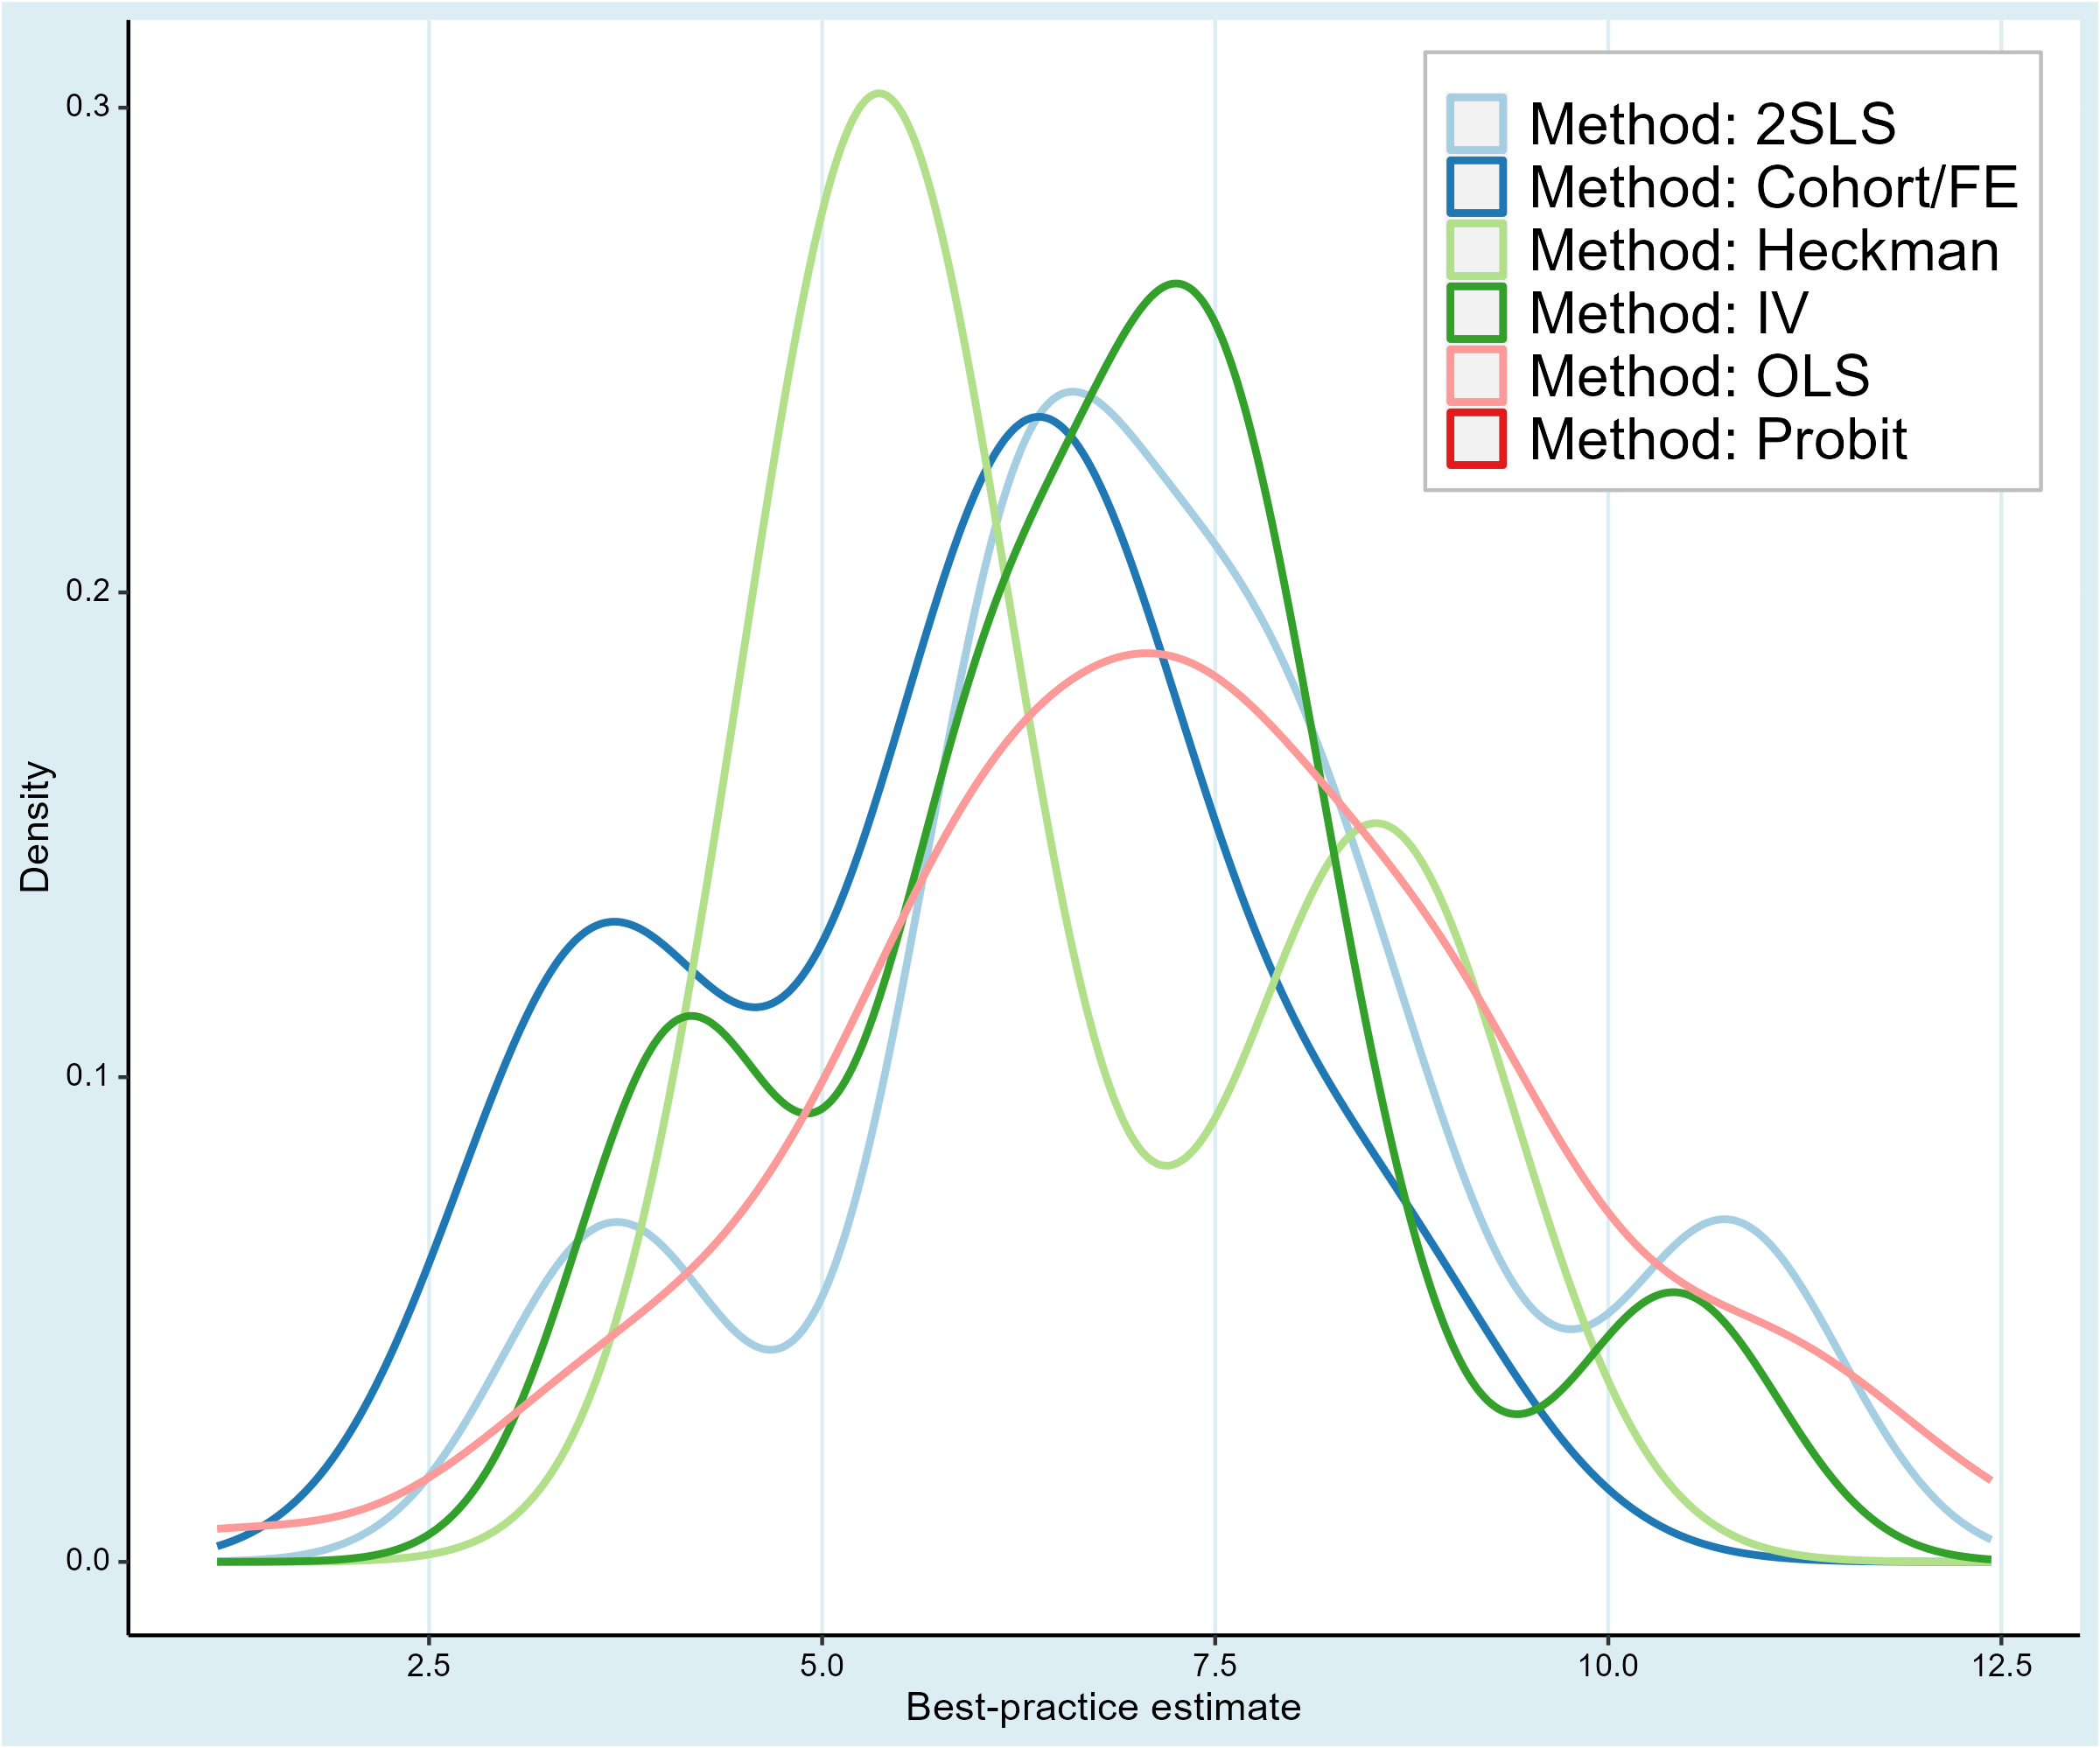
\includegraphics[width=0.95\linewidth]{Figures/BPE/bpe_method.png}
   \label{fig:bpe_method} 
\end{subfigure}

\begin{subfigure}[!htbp]{0.38\textwidth}
   \vspace{0.2cm}
   \caption{Ability}
   \vspace{-0.1cm}
   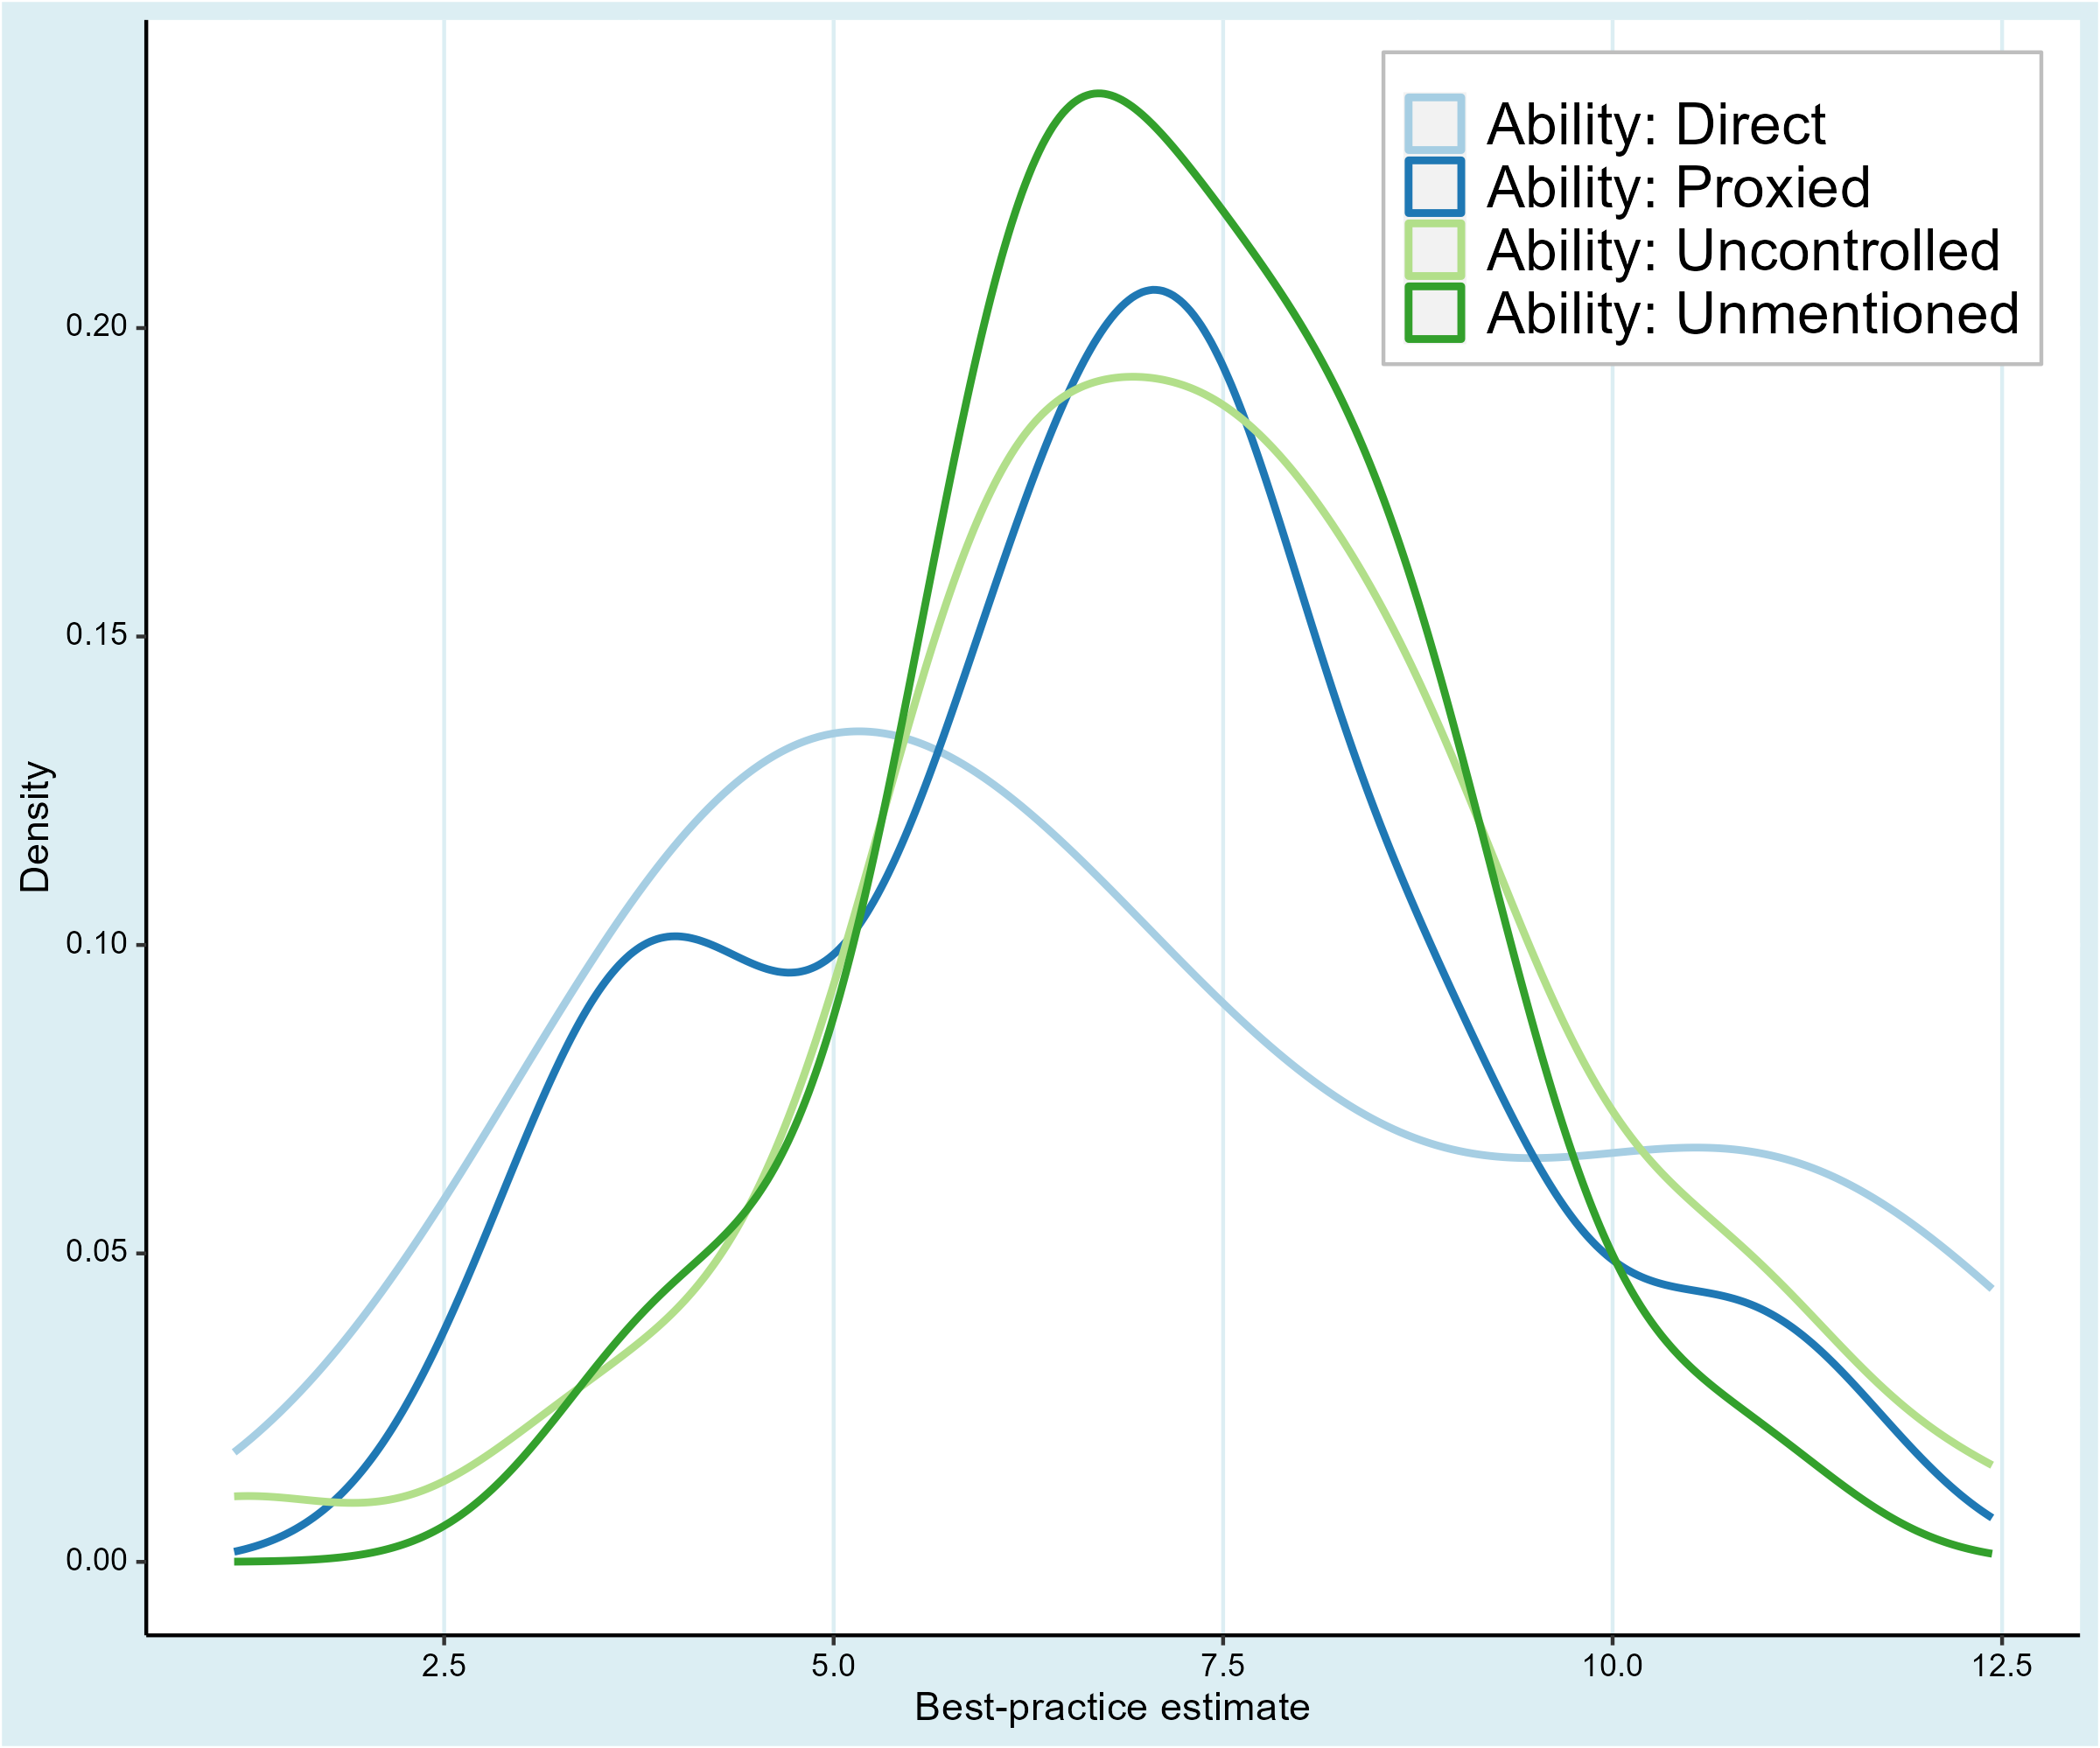
\includegraphics[width=0.95\linewidth]{Figures/BPE/bpe_ability.png}
   \label{fig:bpe_ability}
\end{subfigure}
\begin{subfigure}[!htbp]{0.38\textwidth}
   \vspace{0.2cm}
   \caption{Citations}
   \vspace{-0.1cm}
   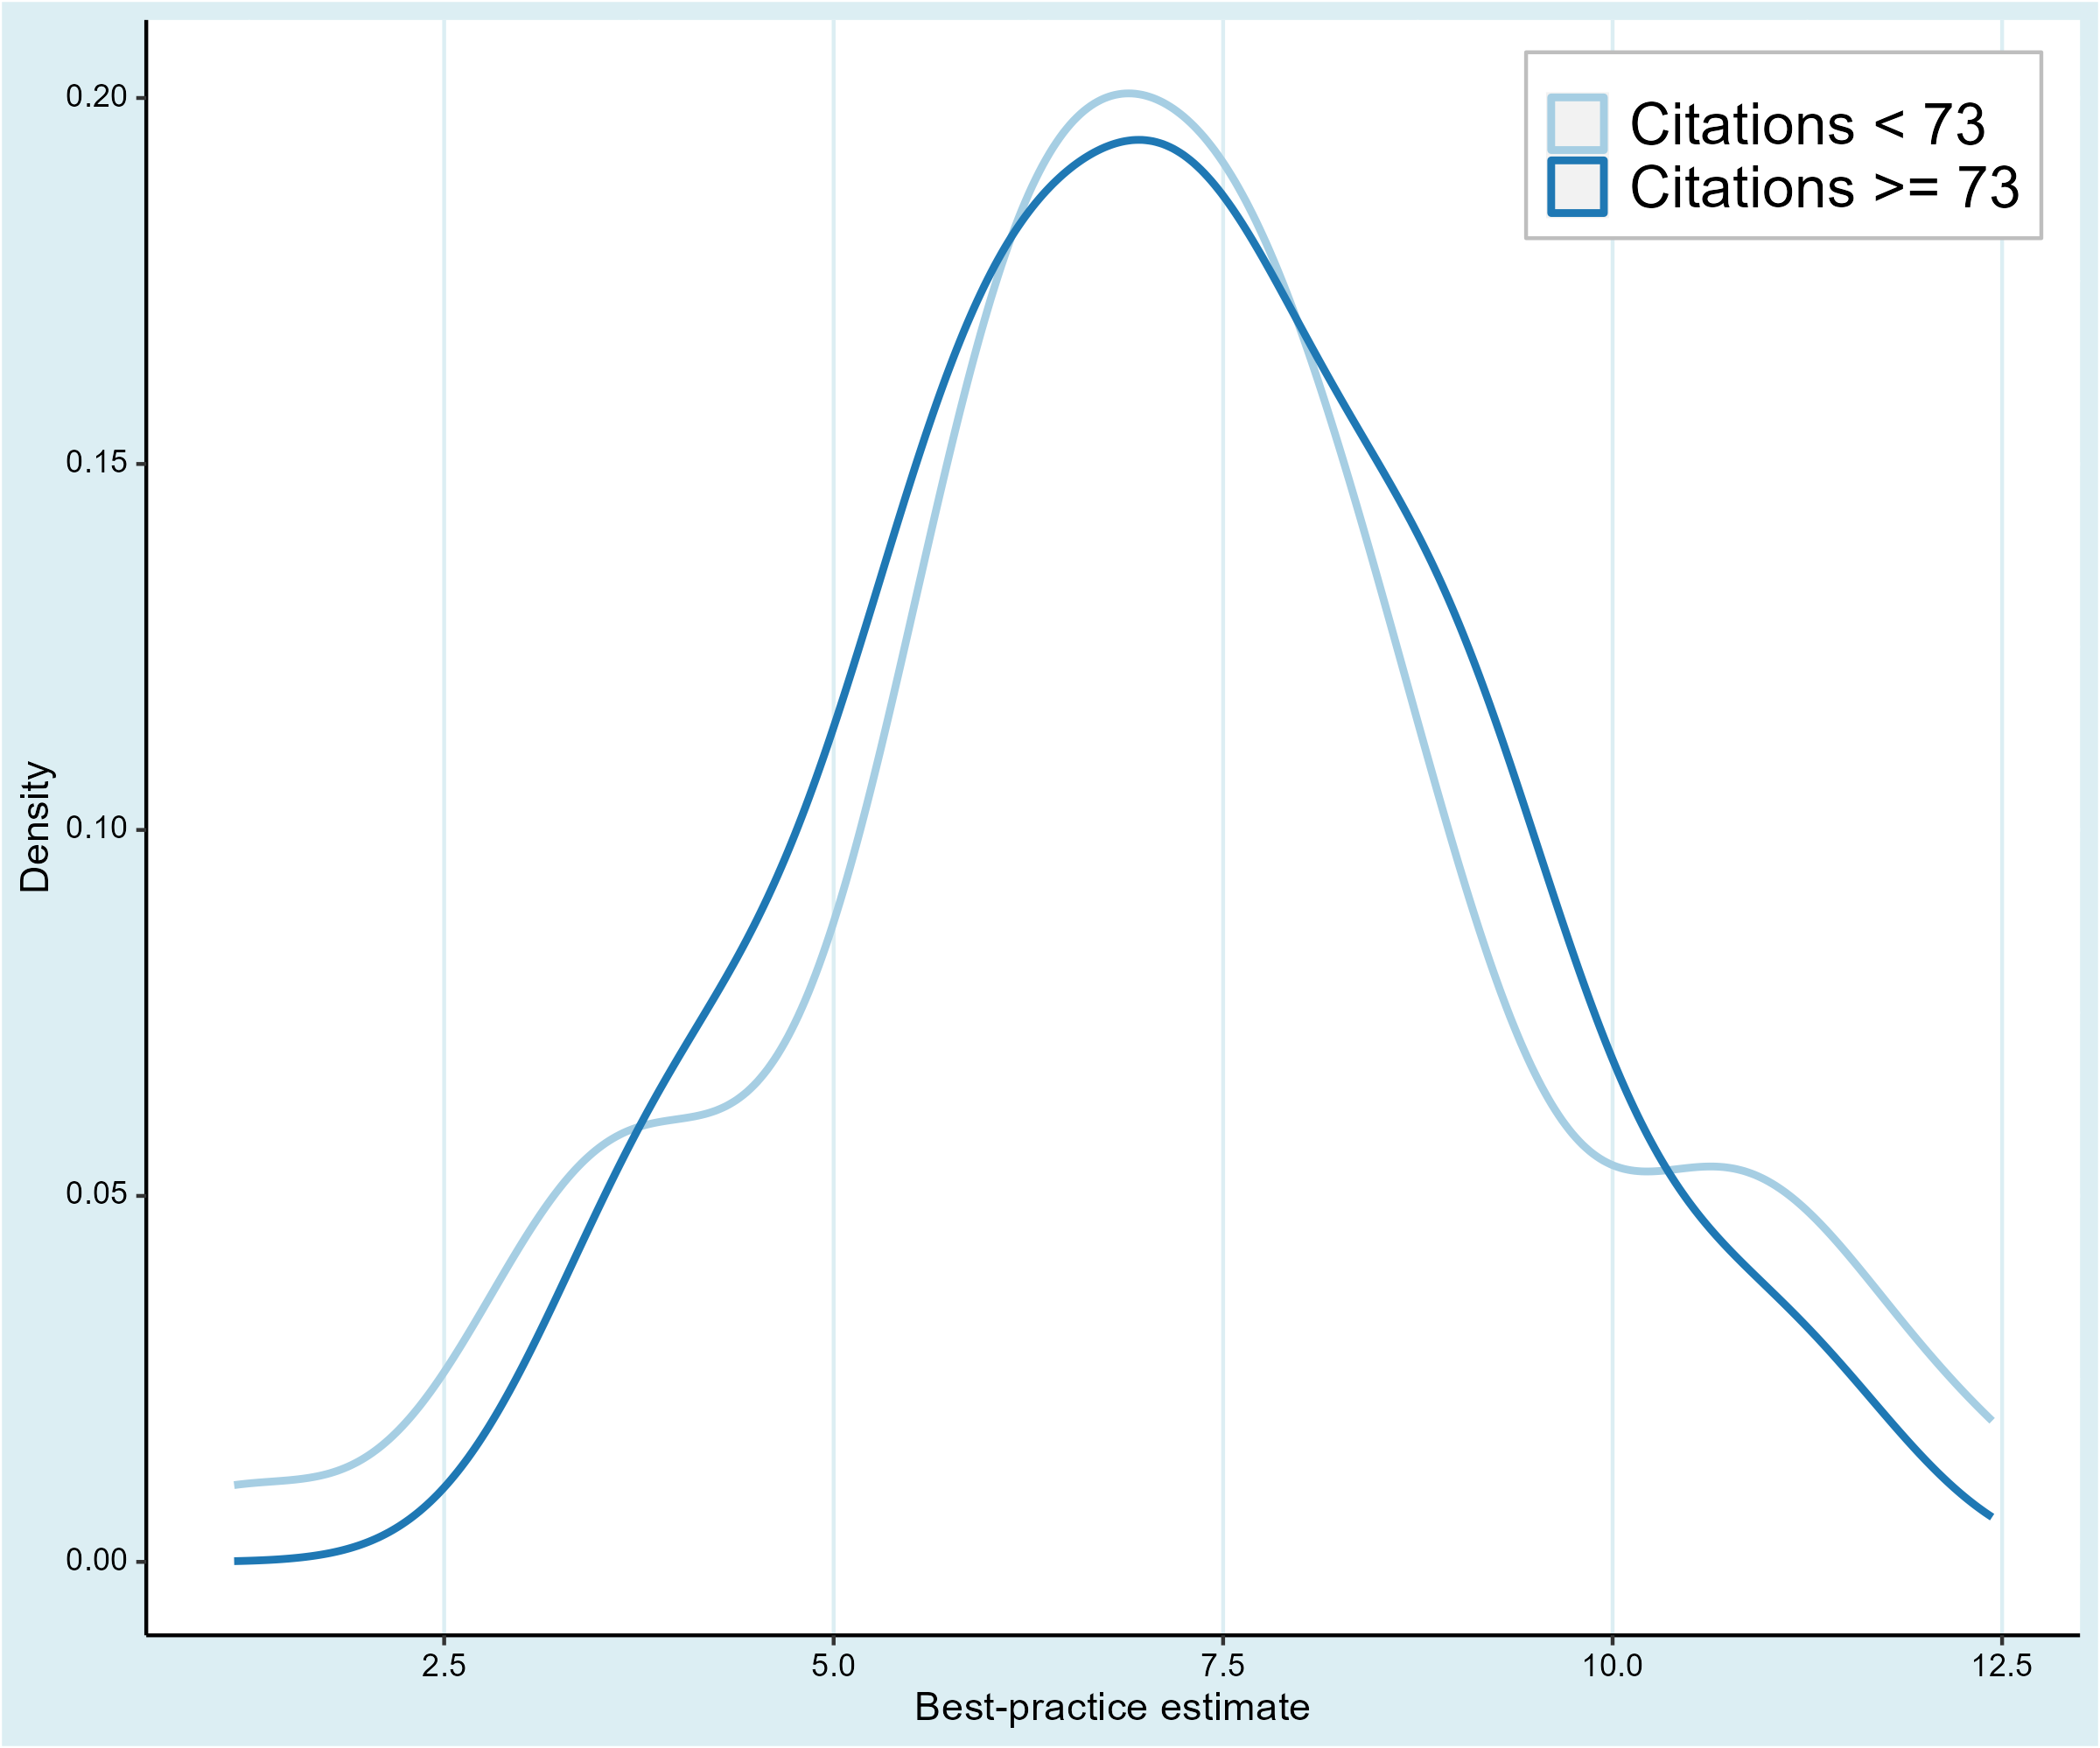
\includegraphics[width=0.95\linewidth]{Figures/BPE/bpe_citations.png}
   \label{fig:bpe_citations}
\end{subfigure}

\end{center}\vspace{-0.6cm}
\captionsetup{width=0.78\textwidth, font = scriptsize}
\caption*{\emph{Note:} This figure displays density lines for best-practice estimates of studies employing different variable setups. Each density line corresponds to a subset of studies whose setup involves a particular variable, as described in each graph's legend. The effect of an additional year of schooling on returns is displayed on the x-axis against its density on the y-axis. For \autoref{fig:bpe_citations}, the data median is used to determine the subsets. For a description of the variables used in these figures, see \autoref{tab:var}.}
\end{figure}

Several crucial points can be drawn from these two sources of information. First and foremost, it is vital to bear in mind the large confidence interval with which nearly all presented estimates and graphs are associated. Despite the lack of confidence bound curves in \autoref{fig:bpe_graphs}, \autoref{tab:bpe_summary_stats} lets us know that the confidence range is quite wide. Second, as I pointed out earlier, the results drawn for data subsets containing only a handful of studies should also be viewed with discretion, as they may be plagued with insufficient data sample bias. 

With these considerations in mind, I dare to point out several intriguing patterns within the results. With 7.109\% returns to education as a baseline average of all best-practice estimates within the literature, some negative deviations appear for studies focusing on uneducated subjects (6.174\%), female subjects (6.388\%), studies employing cohort and fixed-effects estimation (5.861\%) or the Heckman method (6.417\%), and unpublished studies (6.535\%). Regarding ability, studies controlling for it directly or with a proxy report on average lower estimates (6.729\% and 6.873\%, respectively) than studies that omit ability from their models (7.134\% and 7.312\%). As for variables whose employment in study setup causes an increase in estimates, studies with subjects that attained higher education (7.729\%), or were self-employed (8.175\%), stand out among the rest. For the most part, even the differences in means are only marginal and amount to only one or two percentage points in returns at most.

In the graphs, the left-hand side of distributions is visibly more prominent for studies focusing on female subjects or controlling for ability in their models, confirming the numeric findings from \autoref{tab:bpe_summary_stats}. A sizable bump of low percentage estimates also appears in the distribution of estimates for studies focusing on uneducated subjects. Still, due to the low number of studies in this subset, it is likely caused by an anomaly in one or two studies' calculations.

\section{Economic significance}
\label{sec:economic_significance}

Let us now return to the subjective best-practice estimate and consider the role of individual variables again. Namely, I will calculate the economic significance of some prominent variables, which means observing how much each of these variables contributes to the implied best practice when its value is changed. Variables with low \ac{PIP} in the model averaging could be argued to have little impact on the effect in the first place, so for this case, I will be considering only those variables that had \ac{PIP} at least 0.5. In the case of the \ac{BMA} model outlined in \autoref{chap:five}, that totals up to 19 variables. To determine their impact on the effect, I will calculate first how much the implied best-practice changes when there occurs a one standard deviation change in each variable, and then how much that change will be when the variable shifts from its lowest reported value to its highest. The results of these calculations can be found in \autoref{tab:econ_significance}.

% BPE Economic Significance
\begin{table}[!htbp]
   \centering
   \scriptsize
   \singlespace
   \caption{Economic significance of key variables} 
   \label{tab:econ_significance}
   \begin{tabular}{
   @{}
   l
   *{4}{c}
   @{}}
   \toprule
    & \multicolumn{2}{c}{One SD change} & \multicolumn{2}{c}{Maximum change}\\
    & Effect on Returns & \% of BP & Effect on Returns & \% of BP \\
   \midrule
   Standard Error & 0.635 & 9.78\% & 3.399 & 52.37\% \\
   Estimate: Sub-region & -0.442 & -6.81\% & -1.479 & -22.79\% \\
   Estimate: Region & -0.616 & -9.5\% & -1.334 & -20.55\% \\
   Education: Years & 0.554 & 8.53\% & 1.149 & 17.71\% \\
   Wage: Log Hourly & -0.216 & -3.32\% & -0.432 & -6.66\% \\
   Wage: Log Daily & -0.472 & -7.27\% & -1.611 & -24.81\% \\
   Wage: Log Monthly & -0.274 & -4.22\% & -0.671 & -10.34\% \\
   Micro Data & 0.525 & 8.09\% & 1.374 & 21.17\% \\
   Primary Education & 0.522 & 8.04\% & 3.455 & 53.23\% \\
   Higher Education & 1.336 & 20.58\% & 5.397 & 83.14\% \\
   Wage Earners & 0.181 & 2.78\% & 0.882 & 13.59\% \\
   Male & -0.420 & -6.48\% & -1.202 & -18.51\% \\
   Ethnicity: Caucasian & -0.612 & -9.43\% & -1.460 & -22.49\% \\
   Method: 2SLS & 0.449 & 6.91\% & 1.529 & 23.55\% \\
   Method: IV & 0.832 & 12.81\% & 2.651 & 40.84\% \\
   Ability: Direct & -0.416 & -6.41\% & -1.218 & -18.77\% \\
   Ability: Uncontrolled & 0.243 & 3.75\% & 0.492 & 7.58\% \\
   Control: Age & -0.913 & -14.07\% & -1.921 & -29.6\% \\
   Control: Age$^2$ & 1.336 & 20.58\% & 2.992 & 46.1\% \\
   Control: Area & 0.880 & 13.56\% & 1.784 & 27.48\% \\
   Impact Factor & -0.330 & -5.08\% & -1.501 & -23.13\% \\
   Study: Published & -0.491 & -7.57\% & -1.157 & -17.82\% \\
   \bottomrule
   \multicolumn{5}{>{\scriptsize}p{0.8\linewidth}}{\emph{Note:} 
   %XXX REWRITE
   This table shows the individual effect of several important variables on the returns to education, all other things being equal. Variables with \ac{PIP} at least 0.5 are considered important for this matter. One SD change = Change in the effect incurred by a single standard deviation change in the variable. Maximum change = Change in the effect incurred by increasing the variable from its lowest value to its highest. 6.536\% returns to education is the baseline value against which the variables are compared. For an explanation of the variables, see \autoref{tab:var}. SD = Standard deviation, 2SLS = Two-stage Least Squares, IV = Instrumental Variable.}
   \end{tabular}
   \end{table}

With 7.109\% as the reference value of the effect against which the economic significance is compared, there are nine variables with negative influence. In contrast, ten variables pull the effect in the positive direction. Understandably, the standard error is among the variables with a positive sign (0.642 for 1 SD change, 3.435 for maximum change), as an increase in standard error should highly correlate to an increase in the effect. Otherwise, there would have been an unmistakable publication bias in the literature, which the tests in \autoref{chap:four} failed to provide conclusive evidence for. As for the rest of the variables, higher finished education, \ac{IV} regression, age in the quadratic form, and controlling for area display the highest positive impact among the rest. However, the coefficient for the age squared is offset by its linear counterpart, giving the expected convex shape to the Mincer equation and predicting a substantial increase in earnings later in life. Out of the other variables with positive direction, \textit{Education: Years} stands out the most, underlining the suspicion that estimates reporting education in highest achieved levels instead of in years tend to underestimate the returns to education.

As for the variables with a negative influence on the effect, the most significant change is associated with the aforementioned linear age coefficient. Apart from said coefficient, regional and sub-regional level estimates also diminish the overall effect, as does being a male or Caucasian ethnicity. Further, studies with a high impact factor or studies published in journals tend to report higher estimates than their less recognized counterparts. And last but not least, the issue of ability. As has been the case thus far, controlling for ability directly diminishes the overall effect, while leaving the ability out of the equation is associated with higher returns to education. The size of this ability bias, at least when looking at the economic significance of variables, is relatively smaller. Despite this, its presence is unmistakable and in line with all the results presented thus far.
\chapter{Doubling the evidence: Addition of twin studies}
\label{chap:seven}

So far, I have explored the role of schooling and its contribution to an individual's future earnings. Furthermore, I tried to answer the question of what role ability plays in this equation and whether or not it should be accounted for.
Even though I claim that some magnitude of ability bias exists in the relationship, one crucial question remains unanswered. This question is - to what extent is the increase in earnings influenced by schooling and to what extent by ability? Is there a way to separate these two and isolate the effect schooling has on an individual's wage, regardless of their ability? As it turns out, there is. Using a sample of identical twins, one may theoretically rule out the role of ability and family background and observe the unbiased influence of education on earnings. In the following chapter, I attempt to take this approach by constructing an entirely new dataset containing only natural twin studies. With this dataset, I will run the analysis anew and try to determine whether individual differences and innate ability play a crucial role in determining one's future or whether it is all just a matter of education.


\section{Understanding natural experiments: Is it all intertwined?}
\label{sec:twins_literature}

For this analysis, it is vital to understand how being a twin plays a significant role in the matter. We can identify two types of twins - monozygotic and dizygotic. Monozygotic twins (marked further as MZ twins), sometimes called identical twins, come from a single zygote and thus share the same genetic information. For this, it is reasonable to assume they share the same innate ability, and any noteworthy differences that arise during their lifetime should come from their environment, schooling, family background, etc. Dizygotic twins (marked further as DZ twins), on the other hand, come from two different zygotes, and their genetic information thus differs slightly. As such, these may be looked at more as siblings of the same age. For our purposes, monozygotic twins are of particular interest, for if we subset the data to include only these, we can theoretically rule out the role of ability and family background and observe the unbiased influence of education on earnings.

Undoubtedly, this simple line of thinking has its cavetas, as there could still exist bias in the within-twin pair estimators, as pointed out, for example, by \cite{bound1999double}, or \cite{nakamuro2012estimating}. What is more, given that most of the data on twin samples comes from reported estimates, a measurement error could arise in the sample. This is well demonstrated in two of perhaps the most prominent studies in the field, \cite{ashenfelter1994estimates} and \cite{ashenfelter1998income}, where the authors construct a survey and study samples of twins to find that the \ac{OLS} estimate of returns to schooling is upward biased. In \cite{ashenfelter1994estimates}, the authors propose a new approach to combat the measurement error where the measurements of education are collected from both twins, and the final estimate comes from the within-twin comparison. This involves taking one twin's report of the within-twin schooling as an instrument for the other twin's report. The benefit of this approach lies in addressing the possible measurement error that sometimes arises in schooling reports. Several other studies, including \cite{behrman1994endowments}, \cite{isacsson1999estimates}, or \cite{bonjour2003returns}, too follow a similar approach and provide a solid theoretical background to the matter.

Another vital issue, as well as a critique of the twin approach, lies in the idea that the within-twin schooling differences may not be random but endogenous with respect to wages. \cite{bound1999double}, for example, argue that ability can be influenced by factors other than genes and that using methods such as \ac{IV} regression to remedy the measurement error can simultaneously increase the omitted ability bias. On the other hand, using techniques such as Fixed-effects estimator may remove the omitted variable bias but does so at the cost of introducing even greater bias in measurement error \citep{ning2005economic}.

For the purpose of this study, given that its main focus is to determine the extent of the omitted ability bias, I will not explore the issues of measurement error or endogeneity in the twin studies. Instead, holding the simple assumption that ability is inherently the same for identical twins, I will assume that no ability bias exists in the twin data samples. This strong assumption will allow me to directly compare the obtained results to those of the previous chapters, where the omitted ability bias was present. If I discover the results differ, it may further strengthen the notion that the omitted ability bias is indeed present in the data.


\section{What do you mean there are two?: Making a twin dataset}
\label{sec:twins_data}

I will construct the new dataset, comprising natural experiments, with two analysis goals in mind. First, as described in the previous section, I will attempt to quantify the omitted variable bias, and second, I will want to compare the results with the conclusions obtained from the earlier chapters. As such, the form of the dataset will be nearly identical to the one described in \autoref{chap:three}, with slight modifications to accommodate the specific design of the included studies.

As for the studies themselves, I start with the literature review of \cite{nakamuro2012estimating} and \cite{li2012estimating}, and from there, perform snowballing to identify as many relevant studies on the topic as possible. Using this approach, I identified, in total, 16 collectable studies. However, three of these only reported data on mixed samples (both MZ and DZ twins, or MZ twins and non-twins), so I decided to exclude them from the dataset. The remaining 13 studies, which I will use for the analysis, are listed in \autoref{app:one}.  Given how intertwined the studies on the topic are, perhaps due to the relatively small scope of the topic, the choice of which papers to include was somewhat streamlined. Possibly, I may have missed several studies, but I am highly confident that this set should provide a highly representative sample of the literature.

The most important criteria for the selection of each of these studies was for them to feature data on monozygotic twins. Given that most of the papers featured data on dizygotic twins, or non-twins subjects as well, so I decided to collect all available information. However, for the purpose of this analysis, I subset the data only to the observations that concern monozygotic twins. During the collection, it also became apparent that some variables were unusable for this particular use case. Two variables, \textit{Sector: Public/Private}, \textit{Sector: Urban/Rural}, had no observations associated with them at all, while the variables \textit{Control: Experience squared}, \textit{Control: Occupation}, and \textit{Education: Primary/Secondary/...} had fewer than ten. As such, I removed all these variables from the dataset, together with the \textit{Ability} variable, for the approach to measuring ability bias is slightly different now, as explained in \autoref{sec:twins_literature}. For some variable groups, only some sub-categories had no data, such as \textit{Estimate: Sub-region/Continent}, \textit{Micro Data}, \textit{Region: Lat-America/Middle East and North Africa/South Asia/Saharan Africa}, \textit{Income: Low}, \textit{Instrument: Distance to school}, and finally, \textit{Control: Health}. On the other hand, I also added a handful of new variables, including:

\begin{itemize}
  \item \textit{White/Non-white} - Ratio of white subjects to non-white subjects.
  \item \textit{Married/Unmarried} - Ratio of married subjects to non-married subjects.
  \item \textit{Identical/Non-identical/No twins} - Ratio of subjects that are either identical (MZ) or non-identical (DZ) twins or are not twins at all.
  \item \textit{Method: Selection/FE} - =1 if the authors use  Selection-effects or Fixed-effects estimation.
  \item \textit{Method: IV First-differenced} - =1 if the authors use First-Differenced IV estimation.
  \item \textit{Instrument: Smoking} - =1 if the authors use smoking as an instrument in the regression.
\end{itemize}



For the list of all variables used in the analysis and their descriptive statistics, see \autoref{tab:twins_new_vars}. For the list of descriptions of the rest of the variables, see \autoref{tab:var}. The final form of the new dataset includes 154 observations across 13 studies and can be found in the online appendix.


%XXX continue from here



For brevity's sake, I choose not to focus in depth during the analysis on differences between subsets of data, save for the type of method used. However, several statistics that characterize the new group of subjects might be helpful to highlight here just to get a better picture of how this new dataset differs from the old one. Firstly, two-thirds of the data consist of identical twins, roughly 26\% of non-identical twins, and less than 10\% of non-twin subjects. Among these, about 70\% are married, nearly the same amount are white, and over 82\% live in high-income countries. The subjects spent, on average, around 12.4 in school and 17.8 years working. For over 95\% of them, the schooling statistic is reported in years, as opposed to levels. Other statistics, including variable groups capturing data type, estimation method, publication characteristics, etc., can all be found in the aforementioned \autoref{tab:twins_new_vars}.

\begin{table}[!htbp]
  \centering
  \scriptsize
  \singlespace
  \caption{Variables of the twin dataset}
  \label{tab:twins_new_vars}
  \begin{tabular}
    {
      @{\hskip\tabcolsep\extracolsep}
      l
      *{3}{c}
      |
      l
        *{3}{c}
      @{}
    }
    \toprule
    Variable                                                                & Mean   & SD                                                           & Obs   & Variable                                                               & Mean   & SD    & Obs \\
    \midrule
    Effect                                                                  & 6.251  & 2.76                                                         & 293   & Income: High                                                           & 0.823  & 0.383 & 241 \\
    \multicolumn{3}{l}{\textit{\hspace{0.1cm}Estimate characteristics}}     &        & Income: Middle                                               & 0.177 & 0.383                                                                  & 52                   \\
    Standard Error                                                          & 1.126  & 1.036                                                        & 293   & Median Expenditure                                                     & 4.214  & 3.901 & 293 \\
    Estimate: City                                                          & 0.338  & 0.474                                                        & 99    & Minimum Wage                                                           & 3.025  & 2.761 & 293 \\
    Estimate: Region                                                        & 0.055  & 0.228                                                        & 16    & Acad. Freedom Index                                                    & 0.786  & 0.241 & 293 \\
    Estimate: Country                                                       & 0.608  & 0.489                                                        & 178   & Mean Age                                                               & 3.653  & 0.100 & 293 \\
    \multicolumn{3}{l}{\textit{\hspace{0.1cm}Data characteristics}}         &        & \multicolumn{3}{l}{\textit{\hspace{0.1cm}Estimation method}} &                                                                                                       \\
    Study Size                                                              & 3.000  & 0.426                                                        & 293   & Method: OLS                                                            & 0.345  & 0.476 & 101 \\
    Yrs. of Schooling                                                       & 12.463 & 1.456                                                        & 293   & Method: GLS                                                            & 0.102  & 0.304 & 30  \\
    Yrs. of Experience                                                      & 17.875 & 5.627                                                        & 293   & Method: Selection/FE                                                   & 0.253  & 0.435 & 74  \\
    Education: Years                                                        & 0.959  & 0.199                                                        & 281   & Method: FD                                                             & 0.034  & 0.182 & 10  \\
    Education: Levels                                                       & 0.041  & 0.199                                                        & 12    & Method: IV-FD                                                          & 0.068  & 0.253 & 20  \\
    Wage: Hourly                                                            & 0.287  & 0.453                                                        & 84    & Method: IV                                                             & 0.198  & 0.399 & 58  \\
    Wage: Daily                                                             & 0.130  & 0.337                                                        & 38    & Instr.: Sibling Ed.                                                    & 0.140  & 0.348 & 41  \\
    Wage: Monthly/Annual                                                    & 0.584  & 0.494                                                        & 171   & Instr.: Smoking                                                        & 0.061  & 0.241 & 18  \\
    Survey Data                                                             & 0.689  & 0.464                                                        & 202   & Instr.: Other                                                          & 0.048  & 0.214 & 14  \\
    National Register Data                                                  & 0.311  & 0.464                                                        & 91    & Control: Age                                                           & 0.584  & 0.494 & 171 \\
    Cross-sectional Data                                                    & 0.498  & 0.501                                                        & 146   & Control: Age$^2$                                                       & 0.478  & 0.5   & 140 \\
    Panel Data                                                              & 0.502  & 0.501                                                        & 147   & Control: Experience                                                    & 0.218  & 0.414 & 64  \\
    Data Year                                                               & 3.297  & 1.286                                                        & 293   & Control: Ethnicity                                                     & 0.157  & 0.364 & 46  \\
    \multicolumn{3}{l}{\textit{\hspace{0.1cm}Spatial/Structural variation}} &        & Control: Gender                                              & 0.522 & 0.5                                                                    & 153                  \\
    Wage Earners                                                            & 0.962  & 0.052                                                        & 102   & Control: Marriage                                                      & 0.416  & 0.494 & 122 \\
    Gender: Male                                                            & 0.557  & 0.277                                                        & 265   & Control: Firm Char.                                                    & 0.123  & 0.329 & 36  \\
    Gender: Female                                                          & 0.443  & 0.277                                                        & 28    & Control: Area                                                          & 0.055  & 0.228 & 16  \\
    White                                                                   & 0.694  & 0.421                                                        & 190   & Control: Macro Var.                                                    & 0.038  & 0.19  & 11  \\
    Ethnicity: Caucasian                                                    & 0.208  & 0.407                                                        & 61    & \multicolumn{3}{l}{\textit{\hspace{0.1cm}Publication characteristics}} &                      \\
    Married                                                                 & 0.699  & 0.143                                                        & 268   & Impact Factor                                                          & -0.269 & 1.125 & 206 \\
    Unmarried                                                               & 0.301  & 0.143                                                        & 252   & Citations                                                              & 3.855  & 2.173 & 293 \\
    Twins: Identical                                                        & 0.640  & 0.415                                                        & 242   & Study: Published                                                       & 0.703  & 0.458 & 206 \\
    Twins: Non-Identical                                                    & 0.263  & 0.377                                                        & 126   & Study: Unpublished                                                     & 0.297  & 0.458 & 87  \\
    Twins: None                                                             & 0.097  & 0.275                                                        & 34    & Publication Year                                                       & 1.018  & 0.898 & 264 \\
    \bottomrule
    \multicolumn{8}{>{\scriptsize}p{0.9\linewidth}}{\emph{Note:} This table presents basic summary statistics for variables of the new twin dataset. For detailed descriptions of all variables unmentioned in this chapter, see \autoref{tab:var}. SD = Standard Deviation, OLS = Ordinary Least Squares, GLS = Generalized Least Squares, FE = Fixed-Effects, IV = Instrumental Variable.}
  \end{tabular}
\end{table}


\section{Empirical analysis: Are the results just identical?}
\label{sec:twins_analysis}

As far as the outcome of the analysis is concerned, I will focus only on a handful of easily presentable results to keep the chapter concise.  The first is the publication bias issue, which can be summarized in a single table and should not be omitted even from this analysis. In \autoref{tab:PB-Twins}, I present the results of all linear, non-linear, and endogeneity-robust tests and methods explained in \autoref{chap:four}. That is, all but one, as there were too many non-linear techniques to fit into the table nicely; I decided to remove the Hierarchical Bayes results arbitrarily. For clarity, I add that the test for publication bias using said method yielded a coefficient of 0.60 with a standard error of 0.36. In contrast, the coefficient associated with the effect was estimated at 6.85 with a standard error of 0.54 over 293 observations. The rest of the results can be found in the table mentioned above.

% Linear tests
\afterpage{
  \begin{table}[!htbp]
    \centering
    \small
    \singlespace
    \caption{Twin studies are plagued by publication bias}
    \label{tab:PB-Twins}
    \begin{tabular}{
        @{\hskip\tabcolsep\extracolsep}
        l*{5}{c}} %one left column, five center (*{} makes the cols inherit attributes)
      \toprule
      \multicolumn{6}{l}{\textit{Panel A: Linear methods}}                                            \\
      \multicolumn{1}{c}{}                  &
      \textbf{OLS}                          &
      \textbf{FE}                           &
      \textbf{RE}                           &
      \textbf{Study}                        &
      \textbf{Precision}                                                                              \\
      \midrule

      Publication bias                      & 1.347*** & 0.602*** & 0.840*** & 0.947*** & 2.897***    \\
      \emph{\hspace{0.2cm}(Standard error)} & (0.138)  & (0.162)  & (0.154)  & (0.177)  & (0.442)     \\
      \addlinespace[0.5em]
      Effect beyond bias                    & 4.735*** & 5.574*** & 5.55***  & 4.754*** & 3.907***    \\
      \emph{\hspace{0.2cm}(Constant)}       & (0.175)  & (0.219)  & (0.342)  & (0.185)  & (0.232)     \\
      \addlinespace[0.5em]
      Observations                          & 293      & 293      & 293      & 293      & 293         \\

      \midrule

      \multicolumn{6}{l}{\textit{Panel B: Non-linear methods}}                                        \\
                                            &
      \textbf{WAAP}                         &
      \textbf{Top10}                        &
      \textbf{Stem}                         &
      \textbf{AK}                           &
      \textbf{Kink}                                                                                   \\
      \midrule
      Publication bias                      &          &          &          & 2.257*** & 2.895***    \\
                                            &          &          &          & (0.126)  & (0.435)     \\
      \addlinespace[0.5em]
      Effect beyond bias                    & 5.77***  & 4.314*** & 3.403*** & 5.616*** & 3.908***    \\
                                            & (0.159)  & (0.265)  & (0.95)   & (0.157)  & (0.093)     \\
      \addlinespace[0.5em]
      Observations                          & 293      & 293      & 293      & 293      & 293         \\

      \midrule

      \multicolumn{6}{l}{\textit{Panel C: Methods relaxing the exogeneity assumption}}                \\
      \multicolumn{4}{c}{}                  &
      \textbf{IV}                           &
      \textbf{p-uniform*}                                                                             \\
      \midrule
      Publication bias                      &          &          &          & 1.824*** & L = 1.712   \\
                                            &          &          &          & (0.159)  & (p = 0.191) \\
      \addlinespace[0.5em]
      Effect beyond bias                    &          &          &          & 4.198*** & 7.79        \\
                                            &          &          &          & (0.188)  & (NA)        \\
      \addlinespace[0.5em]
      Observations                          &          &          &          & 293      & 293         \\

      \bottomrule
      \multicolumn{6}{>{\footnotesize}p{0.95\linewidth}}{\emph{Note:} Panel A: Results obtained from estimating the linear equation \autoref{eq:fat_reg}. Standard errors, clustered at the study level, are included in parentheses. OLS = Ordinary Least Squares. FE = Fixed Effects. RE = Random Effects. Precision = Estimates are weighted by the inverse of their standard error. Study = Estimates are weighted by the inverse number of observations reported per study. Panel B: Estimates of the effect and publication bias using five non-linear methods. WAAP = Weighted Average of the Adequately Powered \citep{Ioannidis2017Waap}, Top10 = Top10 method by \cite{Stanley2010Top}, Stem = the stem-based method by \cite{Furukawa2019Stem} where P represents the probability of results insignificant at 5\% are published relative to the probability of the significant ones at the same level, AK = \cite{Andrews2019Selection}'s Selection model, Kink = Endogenous kink model by \cite{Bom2019Kink}. Standard errors, clustered at the study level, are included in parentheses. Panel C: Estimates of the effect and publication bias using two techniques that relax the exogeneity assumption. IV = Instrumental Variable Regression; the inverse of the square root of the number of observations is used as an instrument for the standard error. Standard errors, reported in parentheses, are also clustered at the study level. P-uniform* = method proposed by \cite{vanAert2021puni}; L represents the publication bias test t-statistic, the corresponding p-value can be found in parentheses. ***p<0.01, **p<0.05, *p<0.1}
    \end{tabular}
  \end{table}
  \clearpage
}

A clear takeaway from these tests, which also holds across different methods and approaches, is that publication bias is considerably more prominent in the twin dataset than in the primary dataset, as explored in \autoref{chap:four}. With 6.2\% from \autoref{tab:twins_new_vars} as the baseline, the returns to schooling drop by an average of two, sometimes up to three percentage points. Namely, the STEM-based method suggests returns to education of 3.4\%, while the Endogenous Kink approach claims 3.9\%. On the other end of the spectrum, \ac{WAAP} and the Selection model report the highest returns, 5.7\%, and 5.6\%, respectively. No method reports a coefficient of schooling higher than the simple data average, save for p-uniform*, where the standard error failed to be estimated.

Moving on from publication bias, the crux of the matter, which I would like to focus on in terms of analysis outcomes, is the influence of different methods. As outlined in \autoref{sec:twins_literature}, the difference in approach to the omitted ability bias could have us conclude that if the results of the six employed methods vary only a little, the ability bias in the twin studies is not present. On the other hand, if they vary greatly, meaning the estimates of methods controlling for ability are lower than their counterparts, then that would suggest evidence to the contrary.

As a first insight into the influence of different methods on the outcome, I present both numerically and graphically how the returns to education effects behave when employing each of the six methods. In \autoref{fig:twins_prima_facie}, densities of the effect are displayed under different method specifications, while descriptive statistics of the effect behavior under said specifications can be found in \autoref{tab:twins_sum_stats}.

% Include means for subsets of data
\begin{table}[!t]
  \centering
  \scriptsize
  \singlespace
  \caption{Summary statistics for the twin dataset using different estimation methods}
  \label{tab:twins_sum_stats}
  \begin{tabular}{
    @{}
    l % Description
    *{6}{c} % Middle columns
    >{\centering\arraybackslash}p{1cm} % Last column with fixed width
    @{}
    }
    \toprule
                                 & \multicolumn{3}{c}{Unweighted} & \multicolumn{3}{c}{Weighted}        &                                                                      \\
    \cmidrule(lr){2-4} \cmidrule(lr){5-7}
                                 & Mean                           & \multicolumn{2}{c}{95\% conf. int.} & Mean   & \multicolumn{2}{c}{95\% conf. int.} & N. obs                \\

    \midrule


    \multicolumn{8}{l}{\textit{Baseline methods}}                                                                                                                              \\
    Method: OLS                  & 5.686                          & 1.648                               & 9.724  & 5.754                               & 1.716  & 9.792  & 101 \\
    Method: GLS                  & 7.363                          & 1.822                               & 12.904 & 8.005                               & 2.464  & 13.546 & 30  \\
    Method: IV                   & 7.155                          & 1.644                               & 12.666 & 7.570                               & 2.059  & 13.081 & 58  \\
    \midrule
    \multicolumn{8}{l}{\textit{Methods that treat the omitted ability bias}}                                                                                                   \\
    Method: Selection/FE         & 4.917                          & 0.515                               & 9.319  & 5.630                               & 1.228  & 10.032 & 74  \\
    Method: First Differences    & 7.920                          & 3.979                               & 11.861 & 7.916                               & 3.975  & 11.857 & 10  \\
    Method: IV First-Differenced & 8.689                          & 1.035                               & 16.343 & 8.725                               & 1.071  & 16.379 & 20  \\

    \bottomrule

    \multicolumn{8}{>{\scriptsize}p{0.85\linewidth}}{\emph{Note:} This table presents basic summary statistics of the returns to an additional year of schooling coefficient calculated on various subsets of the data. Unweighted = Original dataset is used. Weighted = Estimates are weighted by the inverse number of estimates reported by each study. OLS = Ordinary Least Squares, GLS = Generalised Least Squares, IV = Instrumental Variable, FE = Fixed-Effects. For cutoff points, medians are used except for dummy variables, where the cutoffs are 0.5.}
  \end{tabular}
\end{table}

No obvious pattern appears between the two groups of methods, that is, between the group that does treat the omitted ability bias and the one that does not. While estimates reported by \ac{OLS} and the Selection/Fixed-Effects methods suggest the lowest estimates of all (5.6\% and 4.9\%, respectively), when observing the difference in their estimates as per \cite{li2012estimating}, it comes up to only around 0.7\% (5.6 - 4.9). Even when looking at the weighted average of estimates for these methods, the discrepancies are overall minimal. On balance, this simple glance into the data suggests that treating the ability during the estimation of twin data samples presents only a marginal effect.



% Twins prima facie
\clearpage
\begin{figure}[!htbp]
  \begin{center}
    \caption{Returns to education for twins vary based on the method}
    \label{fig:twins_prima_facie}
    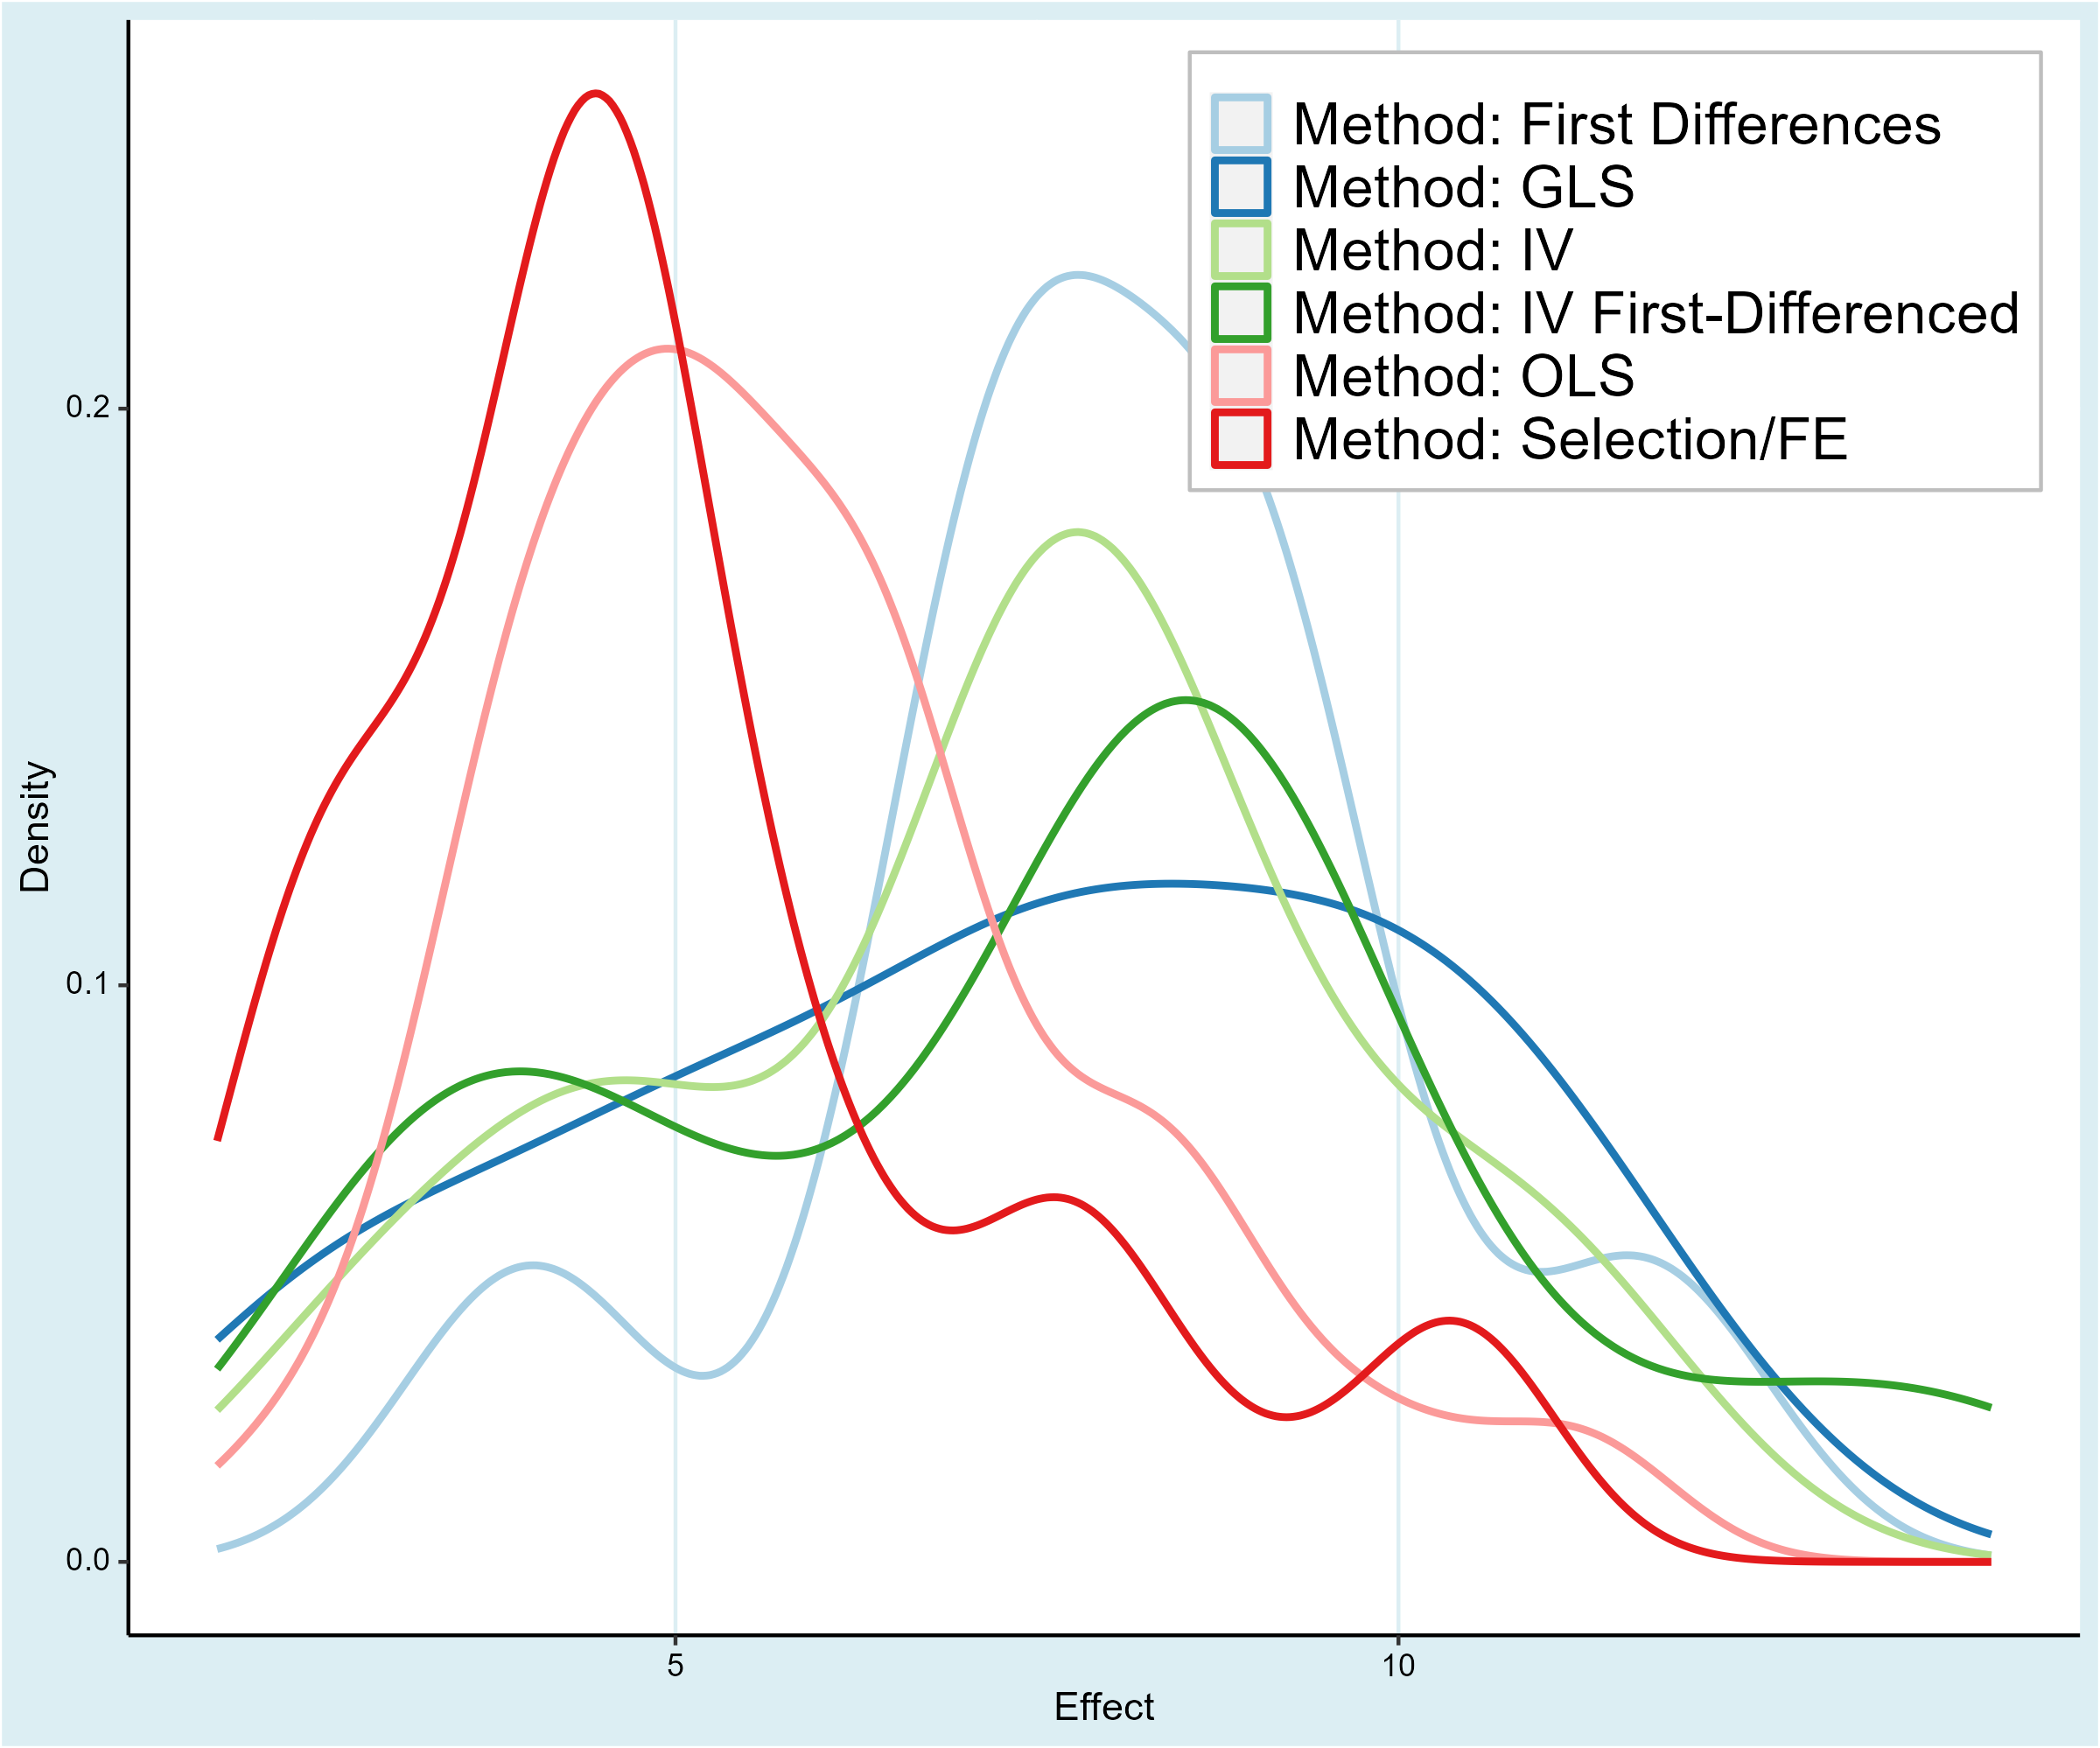
\includegraphics[width=0.9\textwidth]{Figures/twins_prima_method.png}
  \end{center}\vspace{-0.7cm}
  \captionsetup{width=0.9\textwidth, font = scriptsize}
  \caption*{\emph{Note:} This figure displays the densities of the effect of returns to education for twins under different method specifications. The effect is plotted on the x-axis against its density on the y-axis. For a description of the variables used in these figures, refer to \autoref{sec:twins_data}.}
\end{figure}




% Focus on the BMA coefficients for the methods too

% Include a FAT table of fat-pet tests, all on one page, cause no explanations needed - perhaps put in the appendix, dunno

% BPE results and graphs are in order I guess, as are the BMA results


%%%%%%%%%%%%%%%%%%%%%%%%%%%%%%%%%%%%%%%%%%%%%%%%%%%%%%%%%%%%%%%%

%% Notes on theory for self

%Check Li et al. (2012) Appendix Table A1 for concrete figures of ability bias $\to$ omitted variable bias (ability bias) = OLS - FE

%-BMA $\to$ - pub year causing problems, also 10 groups removed using automatic BMA

%Ning (2005) says -> "The
%Fixed-Effect estimator eliminates the omitted variable bias but it does so at the expense of introducing far greater measurement error bias."

%Further, measurement error.
%"A straightforward consistent estimator for equations (6) and (7) or (4) may be obtained by the method of instrumental variables using the independent measure of the schooling variables as instruments". In other words, if the reported schooling is instrumented with the other twins' reported schooling, the measurement error should disappear!!

% Cool twin theory in Bingley et al. (2005)
% A second approach uses within-twins differences in wages and education, assuming that unobserved effects (such as abilities, tastes, motivations, and preferences) are common within twins. However, studies based on siblings or twins have been criticized for two primary reasons. First, if ability consists of both an individual component as well as a family component, which is endogenous to the schooling variable, the within-family approach may not result in estimates that are less biased than OLS estimates. Second, if there is measurement error in the schooling variable, this will account for a large portion of the differences between the twins than across the population as a whole (Ashenfelter et al., 2000).
% KENAYATHULLA, Husaina Banu. "Higher levels of education for higher private returns: New evidence from Malaysia." International Journal of Educational Development, 2013, 33.4: 380-393.
\chapter{Conclusion}
\label{conclusion}

In this thesis, I take a modern look at the relationship between education and earnings with the aim to discover whether and to what extent it is influenced by ability. From a large dataset of 154 studies, I colect 1754 estimates, and through a meticulous scrutiny of the latest meta-analytic research methods, I discover that ability bias is a significant factor in returns to schooling. Contrary to the conventional wisdom, which suggest returns of around 7\%, I propose that the true returns are significantly lower.

As a baseline, I report an average effect of returns to education around 7.4\%, which is very much inline with the previous literature. With this in mind, I run a battery of statistical tests that account for publication bias in the literature, I find that this baseline drops by roughly a full percentage point when publication bias is accounted for. I treat the data for endogeneity, which suggests an even lower effect (around 5.5\%), study structural breaks, and make use of the latest methodology including Elliot's p-hacking tests \citep{elliott2022hacking}, the MAIVE estimator \citep{irsova2023maive}, or the Robust Bayesian Model Averaging \citep{bartovs2023robust}. Although the results of some of the newer methods are mixed, the takeaway idea is that the returns to schooling are in general posioned by a small, but significant publication bias.

To see what role ability and other individual variables play in the picture (of which I collect more than 30), I make use of Bayesian Model Averaging. I find that ability is a highly important factor in determining one's future earnings, and that controlling for ability in the Mincer equation (\citep{mincer1974schooling}) has a significant negative impact on returns to education. Together with this finding, I identify a total of 19 variables that have a large impact on the returns to schooling, including the type of education one attains, their gender, ehtnicity, wage type, or the type of method used to estimate the returns. I run several different specifications of the model, including different model priors, g-priors, etc. to enhance the robustness of my findings.

Next, I calculate a subjective best-practice estimate, which I compare against the best-practice estimates of all individual studies in the dataset, as well as different subsets of these. Here, I mostly observe trends that are in line with the previous findings. To give a more deatiled picture of the results, I pool the best-practice estimates of each study into subsets by their study specifications, allowing me to single out effects of individual variables on returns to schooling. Further, I calculate the economic significance of every variable flagged as important during the Bayesian Model Averaging. These procedures, in general, agree with the results from the previous chapters. In other words, the notion persists that the studies whose authors control for ability, yield, on average, smaller coefficients of returns to education than their counterparts.

As the last, but not insignificant part of the analysis, I collect an entirely new dataset, comprised wholly of experiments whose subjects were identical twins (natural studies), in effort to observe the role of education on earnings in a setting where ability is assumed constant. I find that simply by limiting the pool of subjects to identical twins, the returns to education drop by a full percentage point. When controlling for publication bias, the returns drop even further, to an astonishing two to three percentage points difference.

All in all, I argue that once the data is clear of two important biases (ability and publication), the investment to schooling pays a considerably smaller interest, namely 4-6\% increase in log wage for an additional year spent in school, as opposed to the widely suggested 7\%. This is a crucial finding, as it suggests that the returns to schooling are not as high as previously thought, and that the role of ability in determining one's future earnings is more significant than previously assumed.


However, my approach in getting to these conclusions is not without its faults. Given the limited scope of the thesis, I completely disregard the issue of measurement error and endogeneity when dealing with the natural experiments. Further, I find little time to focus on the implications of inidividual variables, both for the main dataset, and for the twins alike. Given the considerable size and general extent of both of the created datasets, however, further analysis may easily shed more light on issues which I chose, or was forced to overlook within the scope of this thesis.

As the last of my contributions, I would like to mention the existence of an open-source project I created along with this thesis that can be used to quickly and reliably replicate the whole analysis (see \href{https://github.com/PetrCala/Diploma-Thesis}{this link}). Further even, this project allows anyone with a completed meta-analysis dataset to automatically construct their own models, and export the results of these in a compact format that includes \textit{.csv} files, graphs, tables, console logs, and more. With the vast number of methods this tool utilizes, I opted to delve into the inner workings of several of them (including the STEM method by \cite{Furukawa2019Stem}, or the AK model by \cite{Bom2019Kink}), and either improved the speed of their code by a factor of up to 30x, or rewrote the whole methods to allow native execution in the R runtime. All of this creates a seemless user experience for anyone trying to conduct their own meta-analysis.


\clearpage
%-----<<< -------- >>>-----



%-----<<< REFERENCES >>>-----
\fancyhead[LO]{\sffamily Bibliography}					%headers in sans serif and not in uppercase

\bibliographystyle{Styles/newapa.bst}							%style of literature, you can use e.g. newapa	instead of Styles/Stylebib

\bibliography{Styles/Bibliography}							%bibliography database

%input file
\addcontentsline{toc}{chapter}{Bibliography} 		%Add bibliography to the table of contents
\clearpage
%-----<<< ---------- >>>-----


%-----<<< APPENDIXES >>>-----
\backmatter

%uppercase roman pagination for back matter; appendices start

\autohdr																				%automatic headers     
%file with references
\chapter{Literature Exploration}
\label{app:one}

%Notes on the prisma diagram:
% Identification - 574
% Screening - 200
% Eligibility - 122 -> studies excluded due to insufficient data - 48
% Collected - 74

% PRISMA flow diagram
\vspace{-0.4cm}
\begin{figure}[!htbp]
\caption{PRISMA Flow Diagram}
\label{fig:prisma}
\centering
\begin{tikzpicture}[
    node distance=0.9cm,
    start chain=1 going below,
    every join/.style=arrow,
    ]
    % the chain in the center going below
    \coordinate[on chain=1] (tc);
    \node[mynode, on chain=1] (n2)
        {599 records after duplicates removed};
    \node[mynode, join, on chain=1] (n3)
        {255 records screened};
    \node[mynode, join, on chain=1] (n4)
        {119 of full-text articles accessed for eligibility};
    \node[mynode, join, on chain=1] (n5)
        {115 of studies included in the meta-analysis};

    % the branches to the right
    \begin{scope}[start chain=going right]
        \chainin (n3);
        \node[mynode, join, on chain]
            {136 records excluded due to lack of relevance or data};
        \chainin (n4);
        \node[mynode, join, on chain]
            {4 full-text articles excluded due to unfulfilled criteria};
    \end{scope}

    % the nodes at the top  
    \node[mynode, left=0.5cm of tc, anchor=south east] (n1l)
        {574 records identified using Google Scholar query};
    \node[mynode, right=0.5cm of tc, anchor=south west] (n1r) 
        {55 records identified through snowballing};

    \coordinate (n2nl) at ([xshift=-1.5cm]n2.north);
    \coordinate (n2nr) at ([xshift= 1.5cm]n2.north);
    \draw[arrow] (n1l.south -| n2nl) -- (n2nl);
    \draw[arrow] (n1r.south -| n2nr) -- (n2nr);

    % the labels on the left
    \begin{scope}[start chain=going below, xshift=-6cm, yshift=.5cm, node distance=.7cm]
        \node[mylabel, on chain] {\rotatebox{90}{Identification}};
        \node[mylabel, on chain] {\rotatebox{90}{Screening}};
        \node[mylabel, on chain] {\rotatebox{90}{Eligibility}};
        \node[mylabel, on chain] {\rotatebox{90}{Included}};
    \end{scope}

    % the title
    %\node[above=1.5cm of tc, font=\bfseries] {PRISMA 2009 Flow Diagram};
\end{tikzpicture}
\vspace{0.1cm}
\captionsetup{width=0.9\textwidth, font = scriptsize}
\caption*{\emph{Note:} This figure displays a PRISMA flow diagram that graphs the study inclusion process. I use the following Google Scholar query in the search: \textit{\textbf{("ability bias" OR "intelligence bias") AND ("private returns") AND ("income" OR "earnings") AND ("schooling" OR "education")}}. The query search was conducted during a single day on January 23, 2023. The snowballing was conducted roughly a month later. For the list of the 115 studies included in the analysis, see \autoref{tab:studies_query}. PRISMA = Preferred Reporting Items for Systematic Reviews and Meta-Analyses. In constructing the diagram, I follow the advice of \cite{moher2009preferred} and \cite{havranek2020guidelines}.}
\end{figure}


\clearpage
\renewcommand{\arraystretch}{1.1}
\begin{singlespace}
\begin{footnotesize}
\afterpage{\clearpage}
\begin{longtable}[t!]{@{\hskip\tabcolsep}
ll
}
\caption{Studies used in the analysis}  \label{tab:studies_query}\\
\toprule
\endfirsthead
\caption[]{Studies used in the analysis (continued)}\\
\toprule
\endhead
\bottomrule
\multicolumn{2}{r}{{\scriptsize Continued on next page}} \\
\endfoot
\endlastfoot
    \multicolumn{2}{l}{\textit{Panel A: Studies identified by the query}} \\ 
    \cite{acemoglu1999} & \cite{leigh2008returns} \\
    \cite{agrawal2012returns} & \cite{li2007effect} \\
    \cite{arkes2010using} & \cite{lillo2006private} \\
    \cite{aromolaran2006estimates} & \cite{lillo2010rewards} \\
    \cite{aryal2022signaling} & \cite{maluccio1998endogeneity} \\
    \cite{asadullah2006returns} & \cite{mazrekaj2019labour} \\
    \cite{aslam2007rates} & \cite{mishra2012returns} \\
    \cite{ayyash2020returns} & \cite{mishra2014returns} \\
    \cite{bakis2013quantile} & \cite{morgan1998education} \\
    \cite{bartolj2013evolution} & \cite{mphuka2012estimating} \\
    \cite{bergman2018returns} & \cite{okuwa2004private} \\
    \cite{blundell2001estimating} & \cite{patrinos2021private} \\
    \cite{botchorishvili2007private} & \cite{paweenawat2015private} \\
    \cite{campaniello2016returns} & \cite{peters2022course} \\
    \cite{campos2017revisiting} & \cite{purnastuti2013instrumenting} \\
    \cite{casado2005how} & \cite{purnastuti2015returns} \\
    \cite{chanis2021tell} & \cite{qiu2007private} \\
    \cite{debrauw2008reconciling} & \cite{sackey2008private} \\
    \cite{depken2019returns} & \cite{sakellariou2015returns} \\
    \cite{doan2020cost} & \cite{sakellariou2016returns} \\
    \cite{dumauli2015estimate} & \cite{salas2006private} \\
    \cite{fang2012returns} & \cite{salehi2009comparative} \\
    \cite{fersterer2008returns} & \cite{sinning2014much} \\
    \cite{frazer2023firm} & \cite{sinning2017gender} \\
    \cite{gibson2006subsidies} & \cite{sohn2013monetary} \\
    \cite{giles2019great} & \cite{umar2014regional} \\
    \cite{girma2005heterogeneity} & \cite{vanhoeven2013oyedolapo} \\
    \cite{glewwe1996relevance} & \cite{vanpraag2013higher} \\
    \cite{guifu2009economic} & \cite{vasudeva2006returns} \\
    \cite{harmon2002returns} & \cite{vivatsurakit2020returns} \\
    \cite{hawley2004changing} & \cite{walker2008college} \\
    \cite{himaz2016returns} & \cite{wambugu2003essays} \\
    \cite{joseph2020education} & \cite{warunsiri2010returns} \\
    \cite{kenayathulla2013higher} & \cite{webbink2004returns} \\
    \cite{kolstad2015education} & \cite{wincenciak2020evolution} \\
    \cite{krafft2018school} & \cite{zhong2011returns} \\
    \cite{krafft2019what} & \cite{zhu2012economic} \\
    \midrule
    \multicolumn{2}{l}{\textit{Panel B: Studies identified by snowballing}} \\ 
    \cite{aakvik2010measuring} & \cite{heckman2006earnings} \\
    \cite{angrist1995economic} & \cite{hubbard2011phantom} \\
    \cite{angrist1991compulsory} & \cite{ichino1999lower} \\
    \cite{belzil2002unobserved} & \cite{ichino2004long} \\
    \cite{brainerd1998winners} & \cite{jones2001educated} \\
    \cite{breda2014firms} & \cite{kane1993labor} \\
    \cite{capatina2014skills} & \cite{kijima2006why} \\
    \cite{card1995using} & \cite{kingdon1998does} \\
    \cite{carneiro2011estimating} & \cite{leigh2008estimating} \\
    \cite{chase1998markets} & \cite{lemieux2001education} \\
    \cite{devereux2010forced} & \cite{light2004receives} \\
    \cite{dougherty1991specification} & \cite{moretti2004estimating} \\
    \cite{duflo2001schooling} & \cite{munich2005returns} \\
    \cite{duraisamy2002changes} & \cite{pischke2005zero} \\
    \cite{fortin2008gender} & \cite{psacharopoulos1982earnings} \\
    \cite{gill2000community} & \cite{psacharopoulos1979human} \\
    \cite{gorodnichenko2005returns} & \cite{staiger1997instrumental} \\
    \cite{grogger1995changes} & \cite{stephens2014compulsory} \\
    \cite{harmon1995estimates} & \cite{taber2001rising} \\
    \cite{harmon1999marginal} & \cite{troske1999evidence} \\   
    \midrule
    \multicolumn{2}{l}{\textit{Panel C: Twin studies}} \\ 
    \cite{ashenfelter1994estimates} & \cite{isacsson1999estimates} \\
    \cite{ashenfelter1998income} & \cite{isacsson2004estimating} \\
    \cite{behrman1994endowments} & \cite{li2012estimating} \\
    \cite{behrman1999ability} & \cite{miller1995twins} \\
    \cite{bingley2009returns} & \cite{miller2004test} \\
    \cite{blanchflower1999ability} & \cite{nakamuro2012estimating} \\
    \cite{bonjour2003returns} & \cite{ning2005economic} \\
    \cite{feigenbaum2020return} & \cite{rouse1999further} \\
\bottomrule
\multicolumn{2}{>{\scriptsize}p{0.9\linewidth}}{\emph{Note:} This table lists all studies used in the analysis. Panel A shows 74 studies identified by the main Google Scholar query; panel B shows 41 studies identified by snowballing. These two panels together present 115 studies from the main dataset, explored in \autoref{chap:three}. Panel C displays 16 studies from the twin dataset, explored in \autoref{chap:seven}.}
\end{longtable}
\end{footnotesize}
\end{singlespace}
%}

\begin{figure}[!htbp]
\begin{center}
\caption{Box plot of estimates across countries}
\label{fig:box_plot_countries}
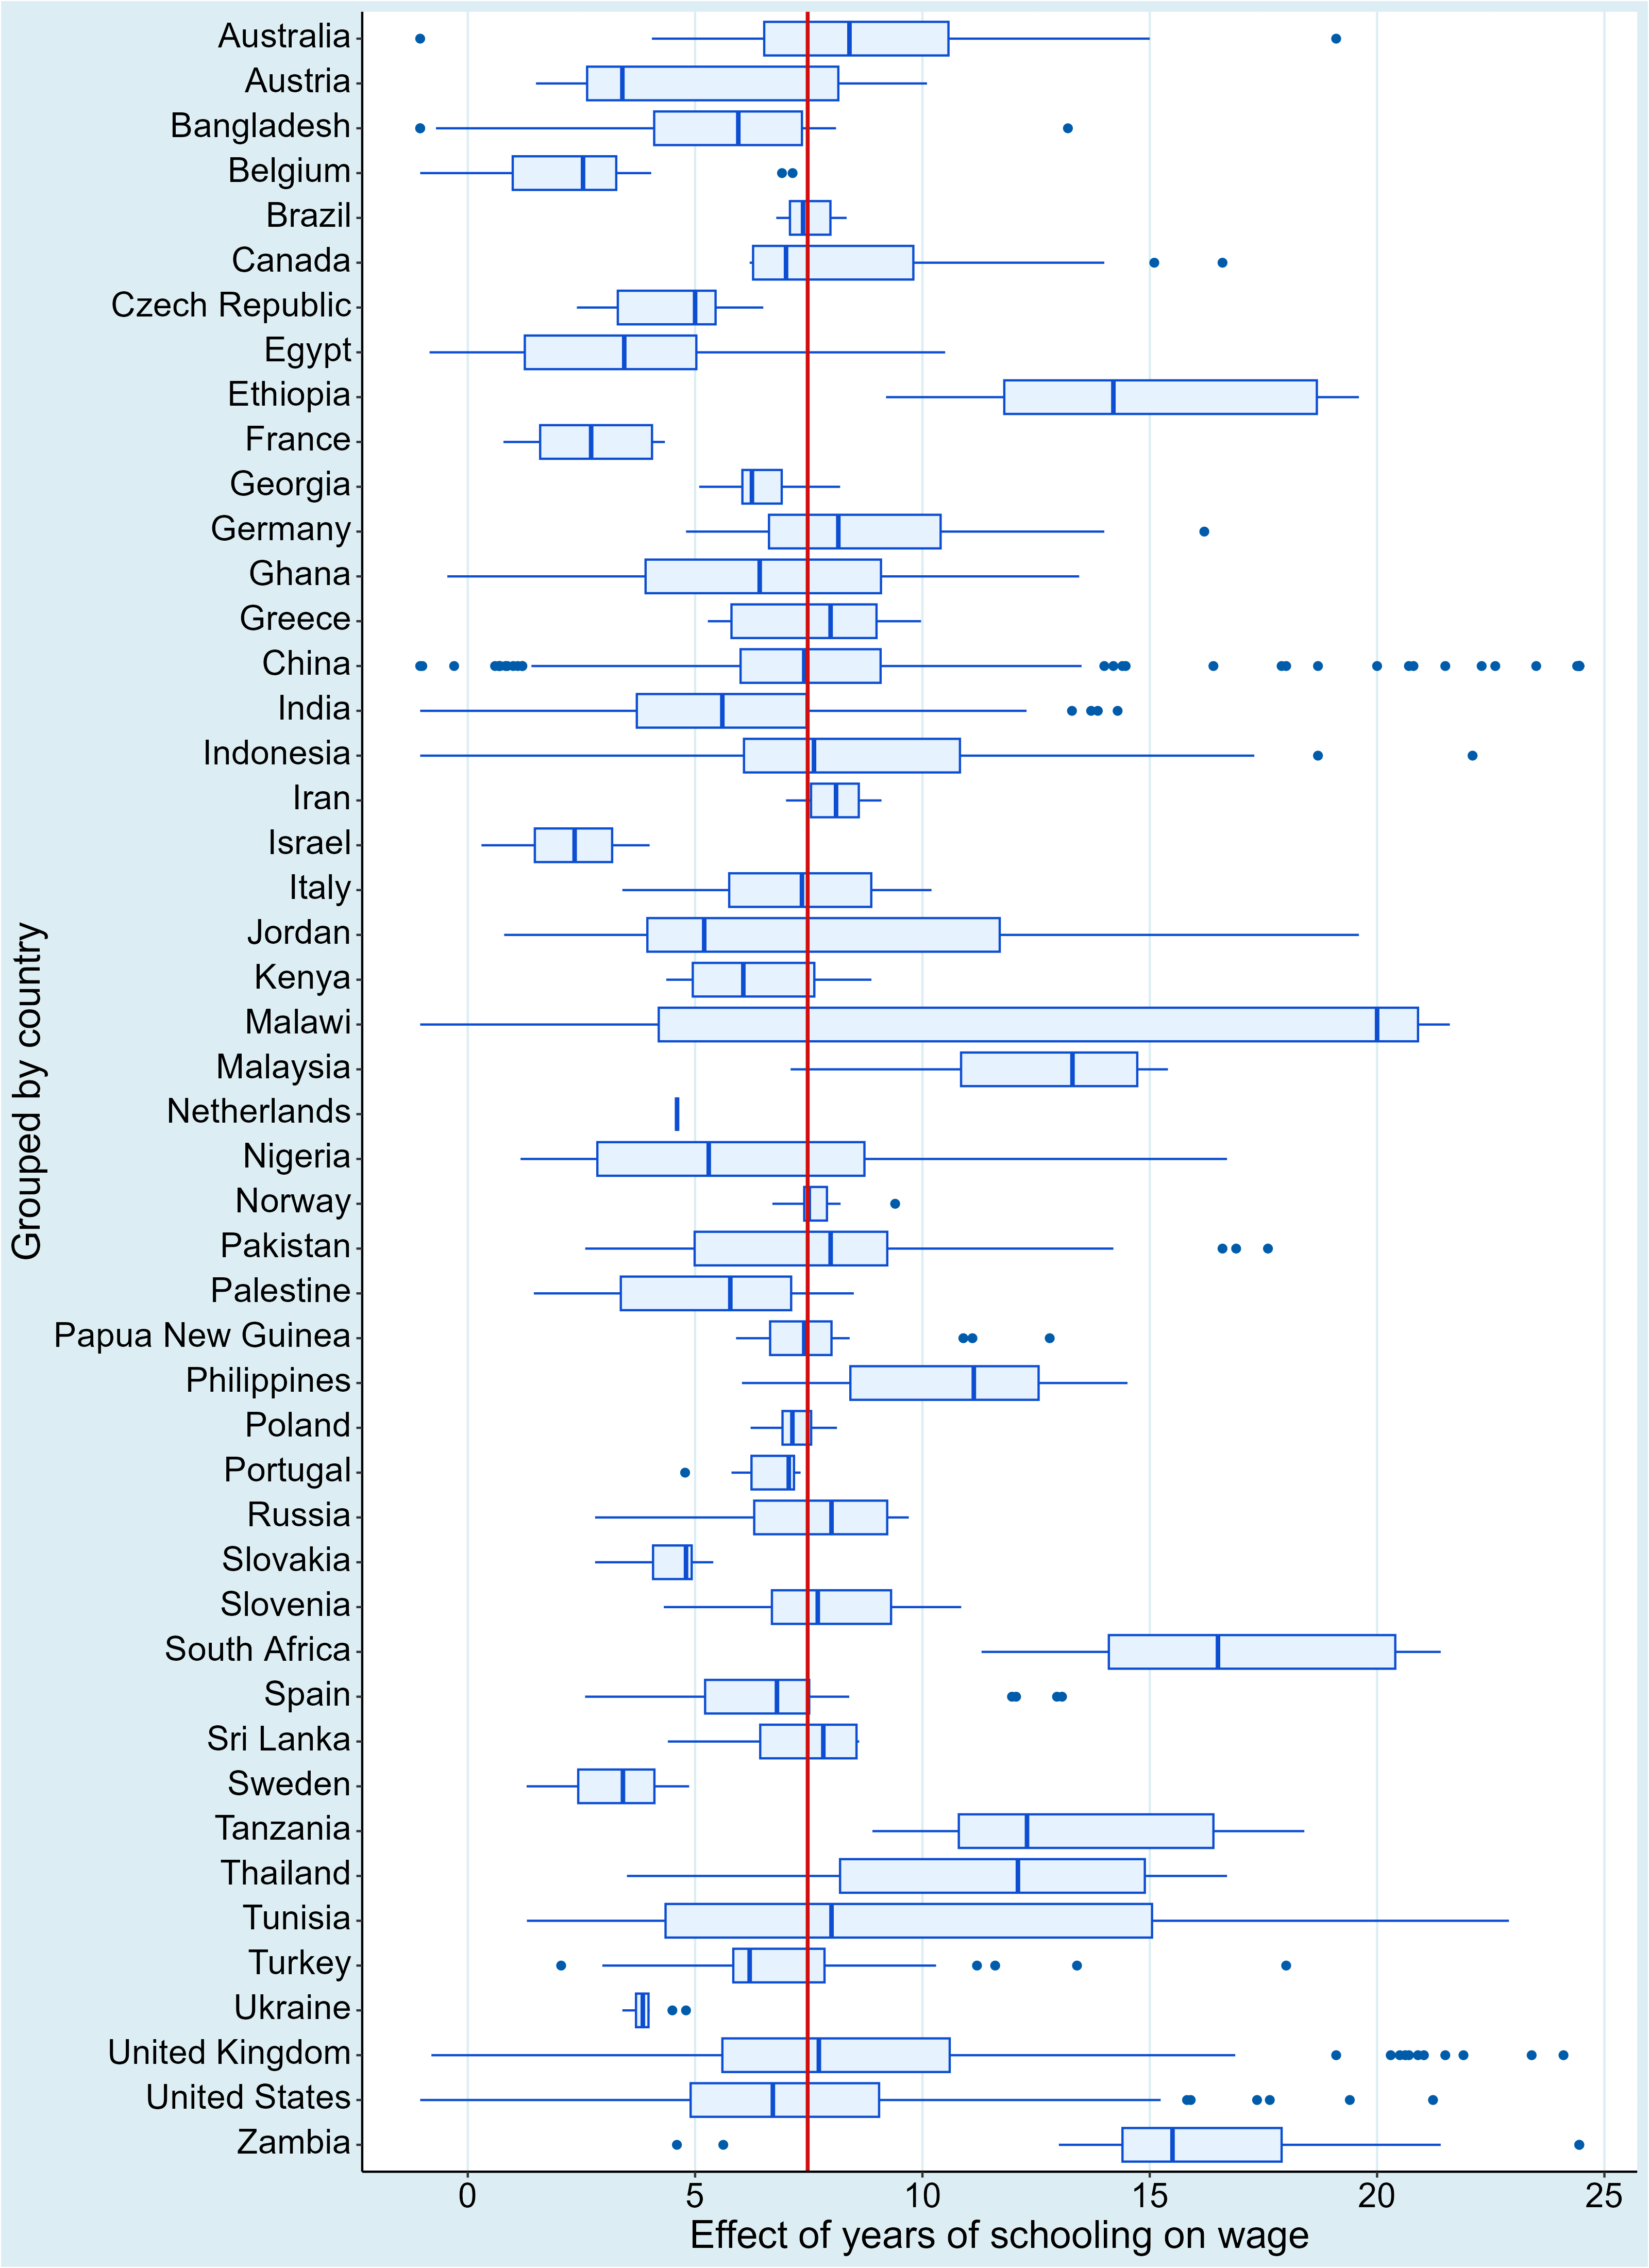
\includegraphics[width=0.9\textwidth]{Figures/box_plot_country.png}
\end{center}\vspace{-0.7cm}
\captionsetup{width=0.9\textwidth, font = scriptsize}
\caption*{\emph{Note:} This figure shows a box plot where the reported estimates are grouped at the country level. The data of all 48 countries from the data set is displayed. The red line represents the average effect across the literature. Each box's length represents the interquartile range between the 25th and 75th percentiles. The dividing line within each box indicates the median value. The whiskers extend to the highest and lowest data points within 1.5 times the range between the upper and lower quartiles. Outliers are depicted as blue dots. The data is winsorized at 1\% level.}
\end{figure}
           			%List of studies
\chapter{Bayesian model averaging robustness check}
\label{app:three}

\begin{figure}[!htbp]
\begin{center}
\caption{BMA - uniform g-prior and uniform model prior}
\label{fig:BMA2}
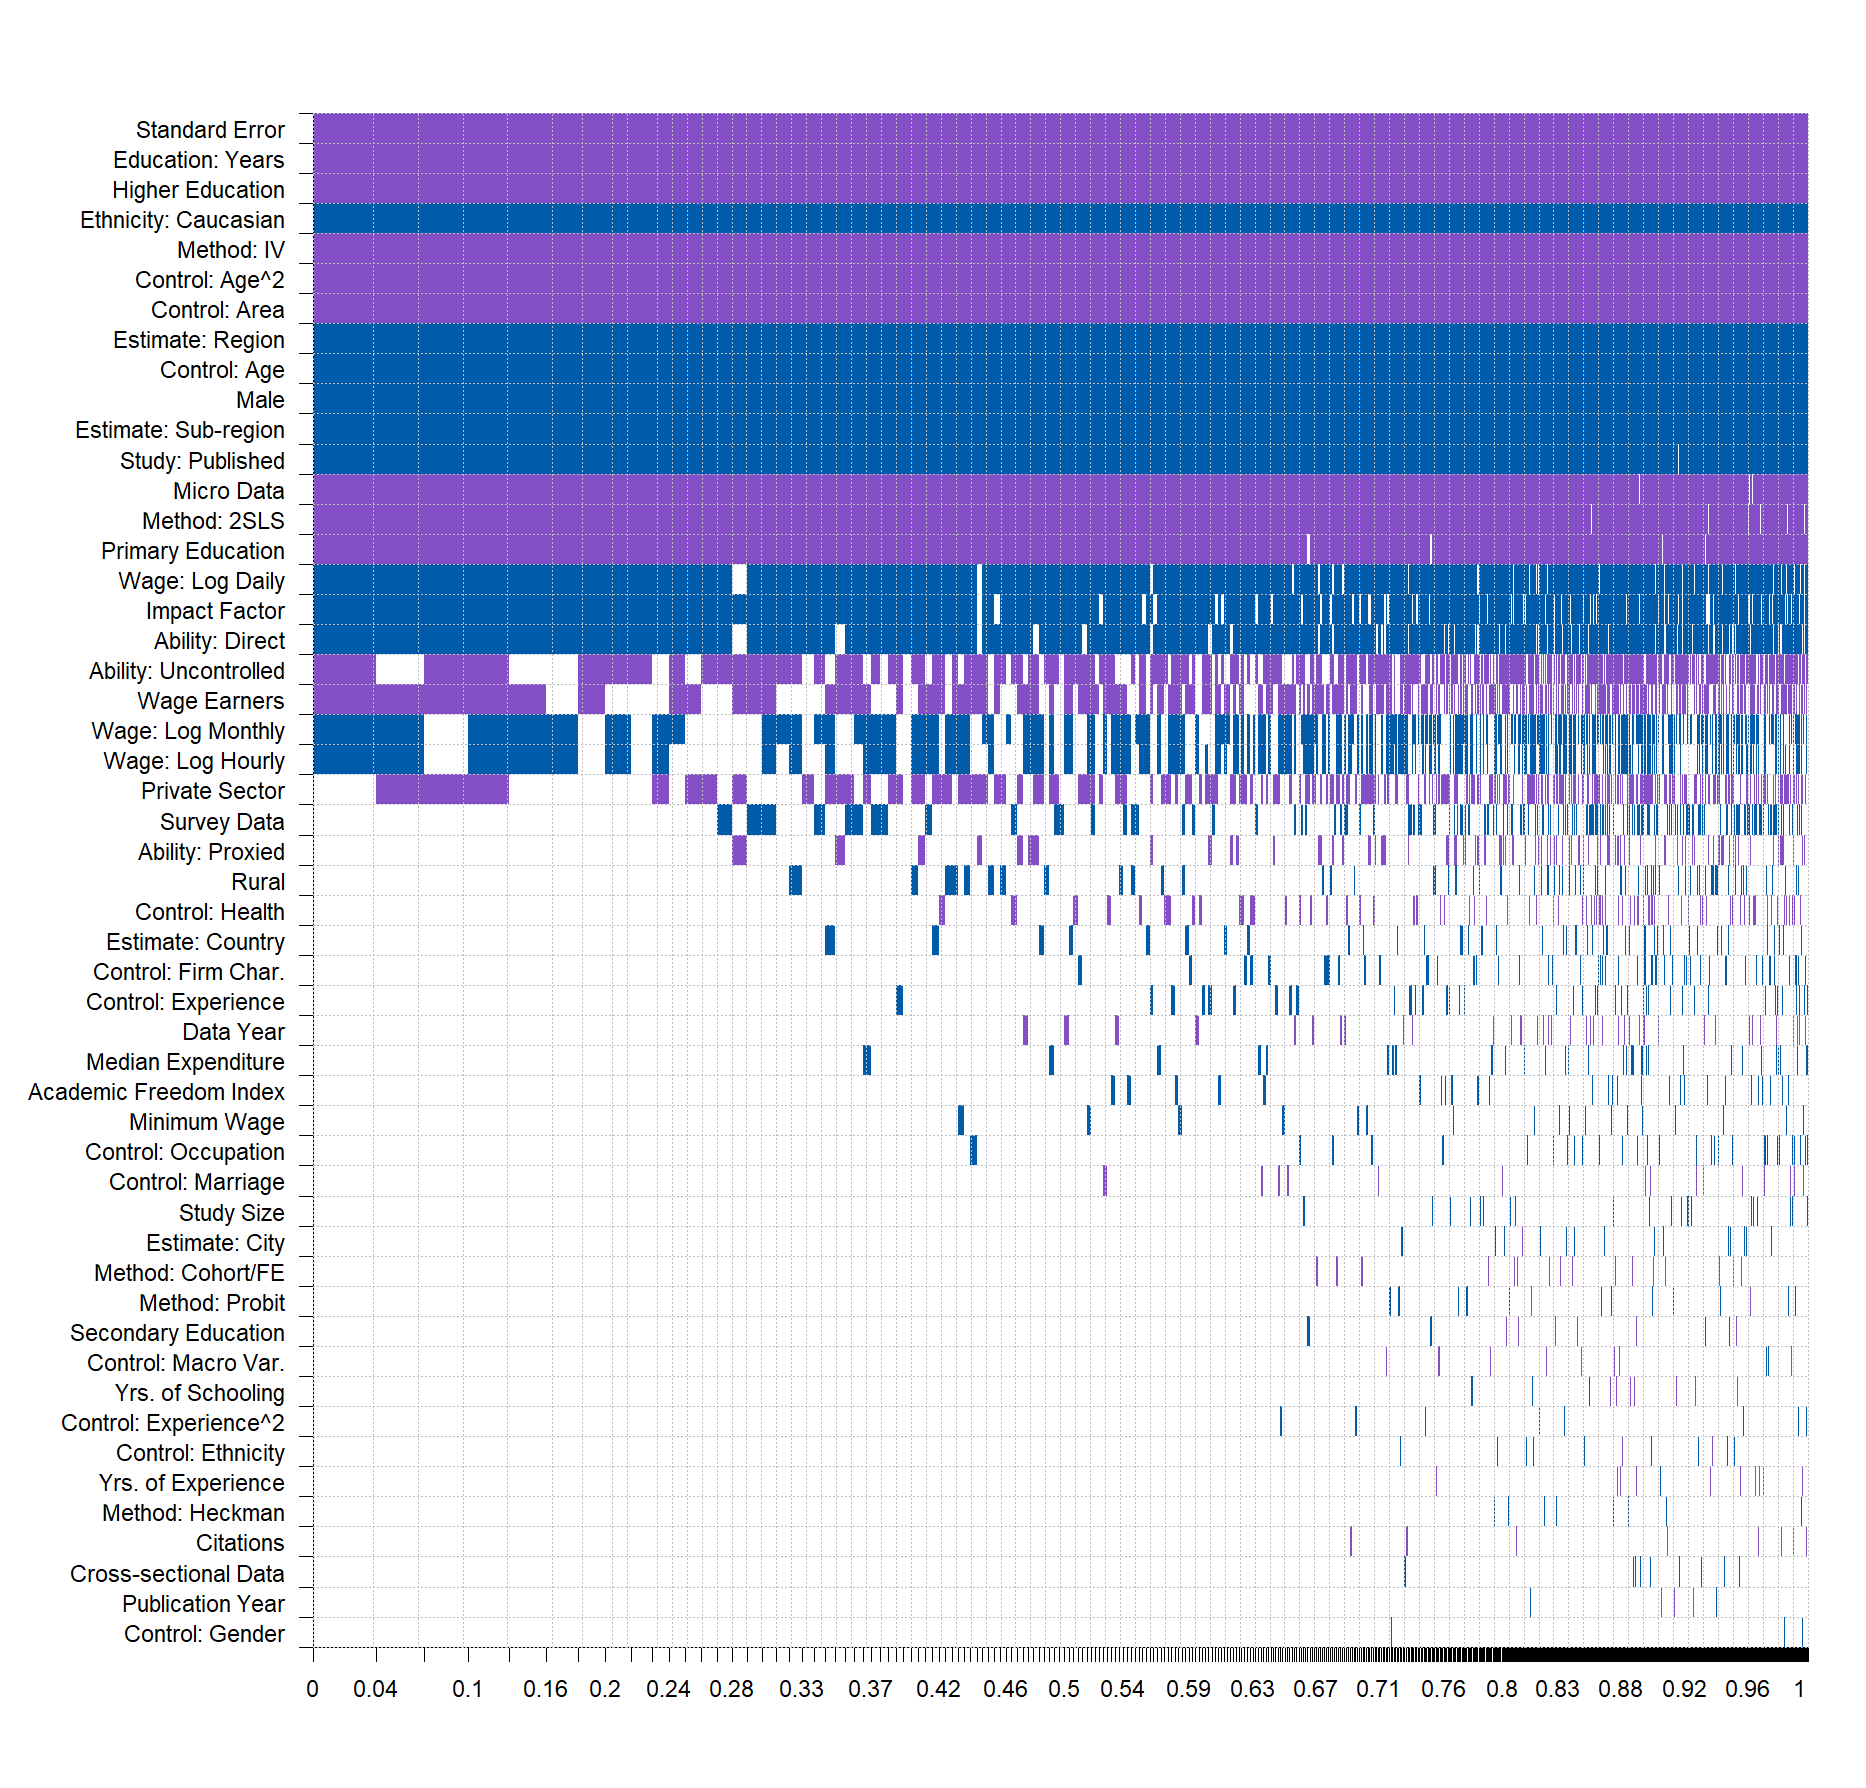
\includegraphics[width=0.8\textwidth]{Figures/BMA/bma_UIP_uniform_results.png}
\end{center}\vspace{-0.5cm}
\captionsetup{width=0.8\textwidth, font = scriptsize}
\caption*{\emph{Note:} This figure unveils the results of running the Bayesian model averaging using different specifications, namely the uniform g-prior and the uniform model prior. BMA = Bayesian model averaging. For further explanation of the procedure and individual variables, see \autoref{fig:BMA} and \autoref{tab:var}.
}
\end{figure}


\begin{figure}[!htbp]
\begin{center}
\caption{BMA - benchmark g-prior and random model prior}
\label{fig:BMA3}
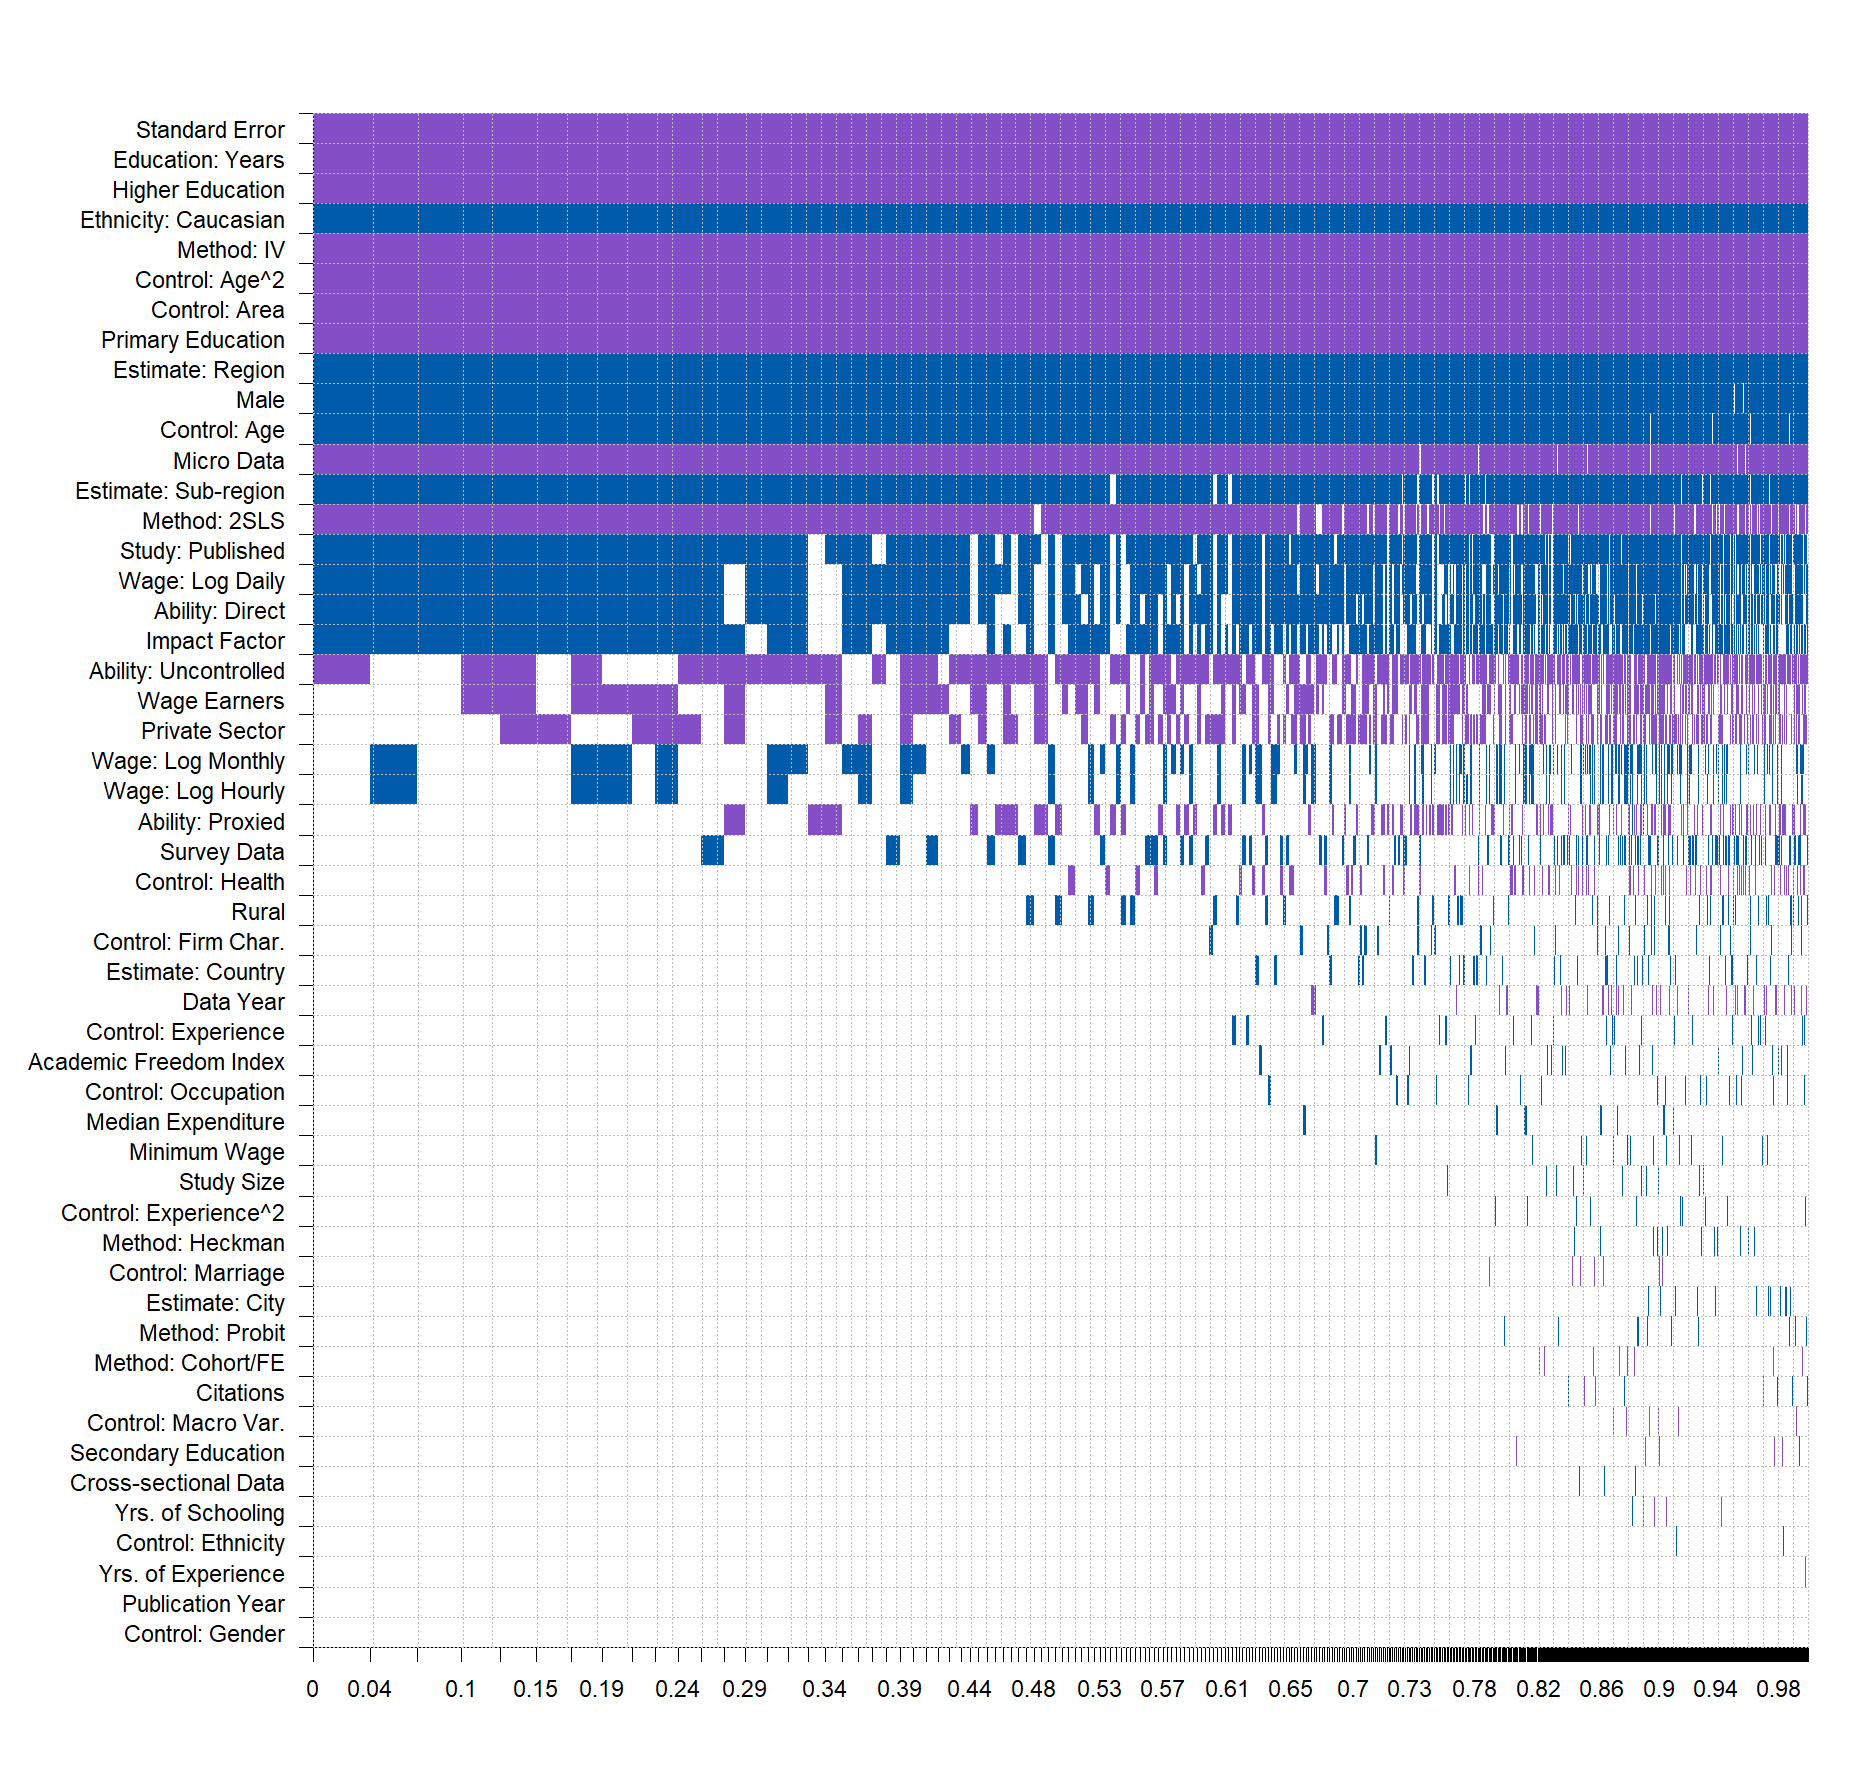
\includegraphics[width=0.9\textwidth]{Figures/BMA/bma_BRIC_random_results.png}
\end{center}\vspace{-0.5cm}
\captionsetup{width=0.9\textwidth, font = scriptsize}
\caption*{\emph{Note:} This figure unveils the results of running the Bayesian model averaging using different specifications, namely the benchmark g-prior and the uniform model prior. BMA = Bayesian model averaging. For further explanation of the method and the employed variables, see \autoref{fig:BMA} and \autoref{tab:var}.
}
\end{figure}

\begin{figure}[!htbp]
\begin{center}
\caption{BMA - HQ g-prior and random model prior}
\label{fig:BMA4}
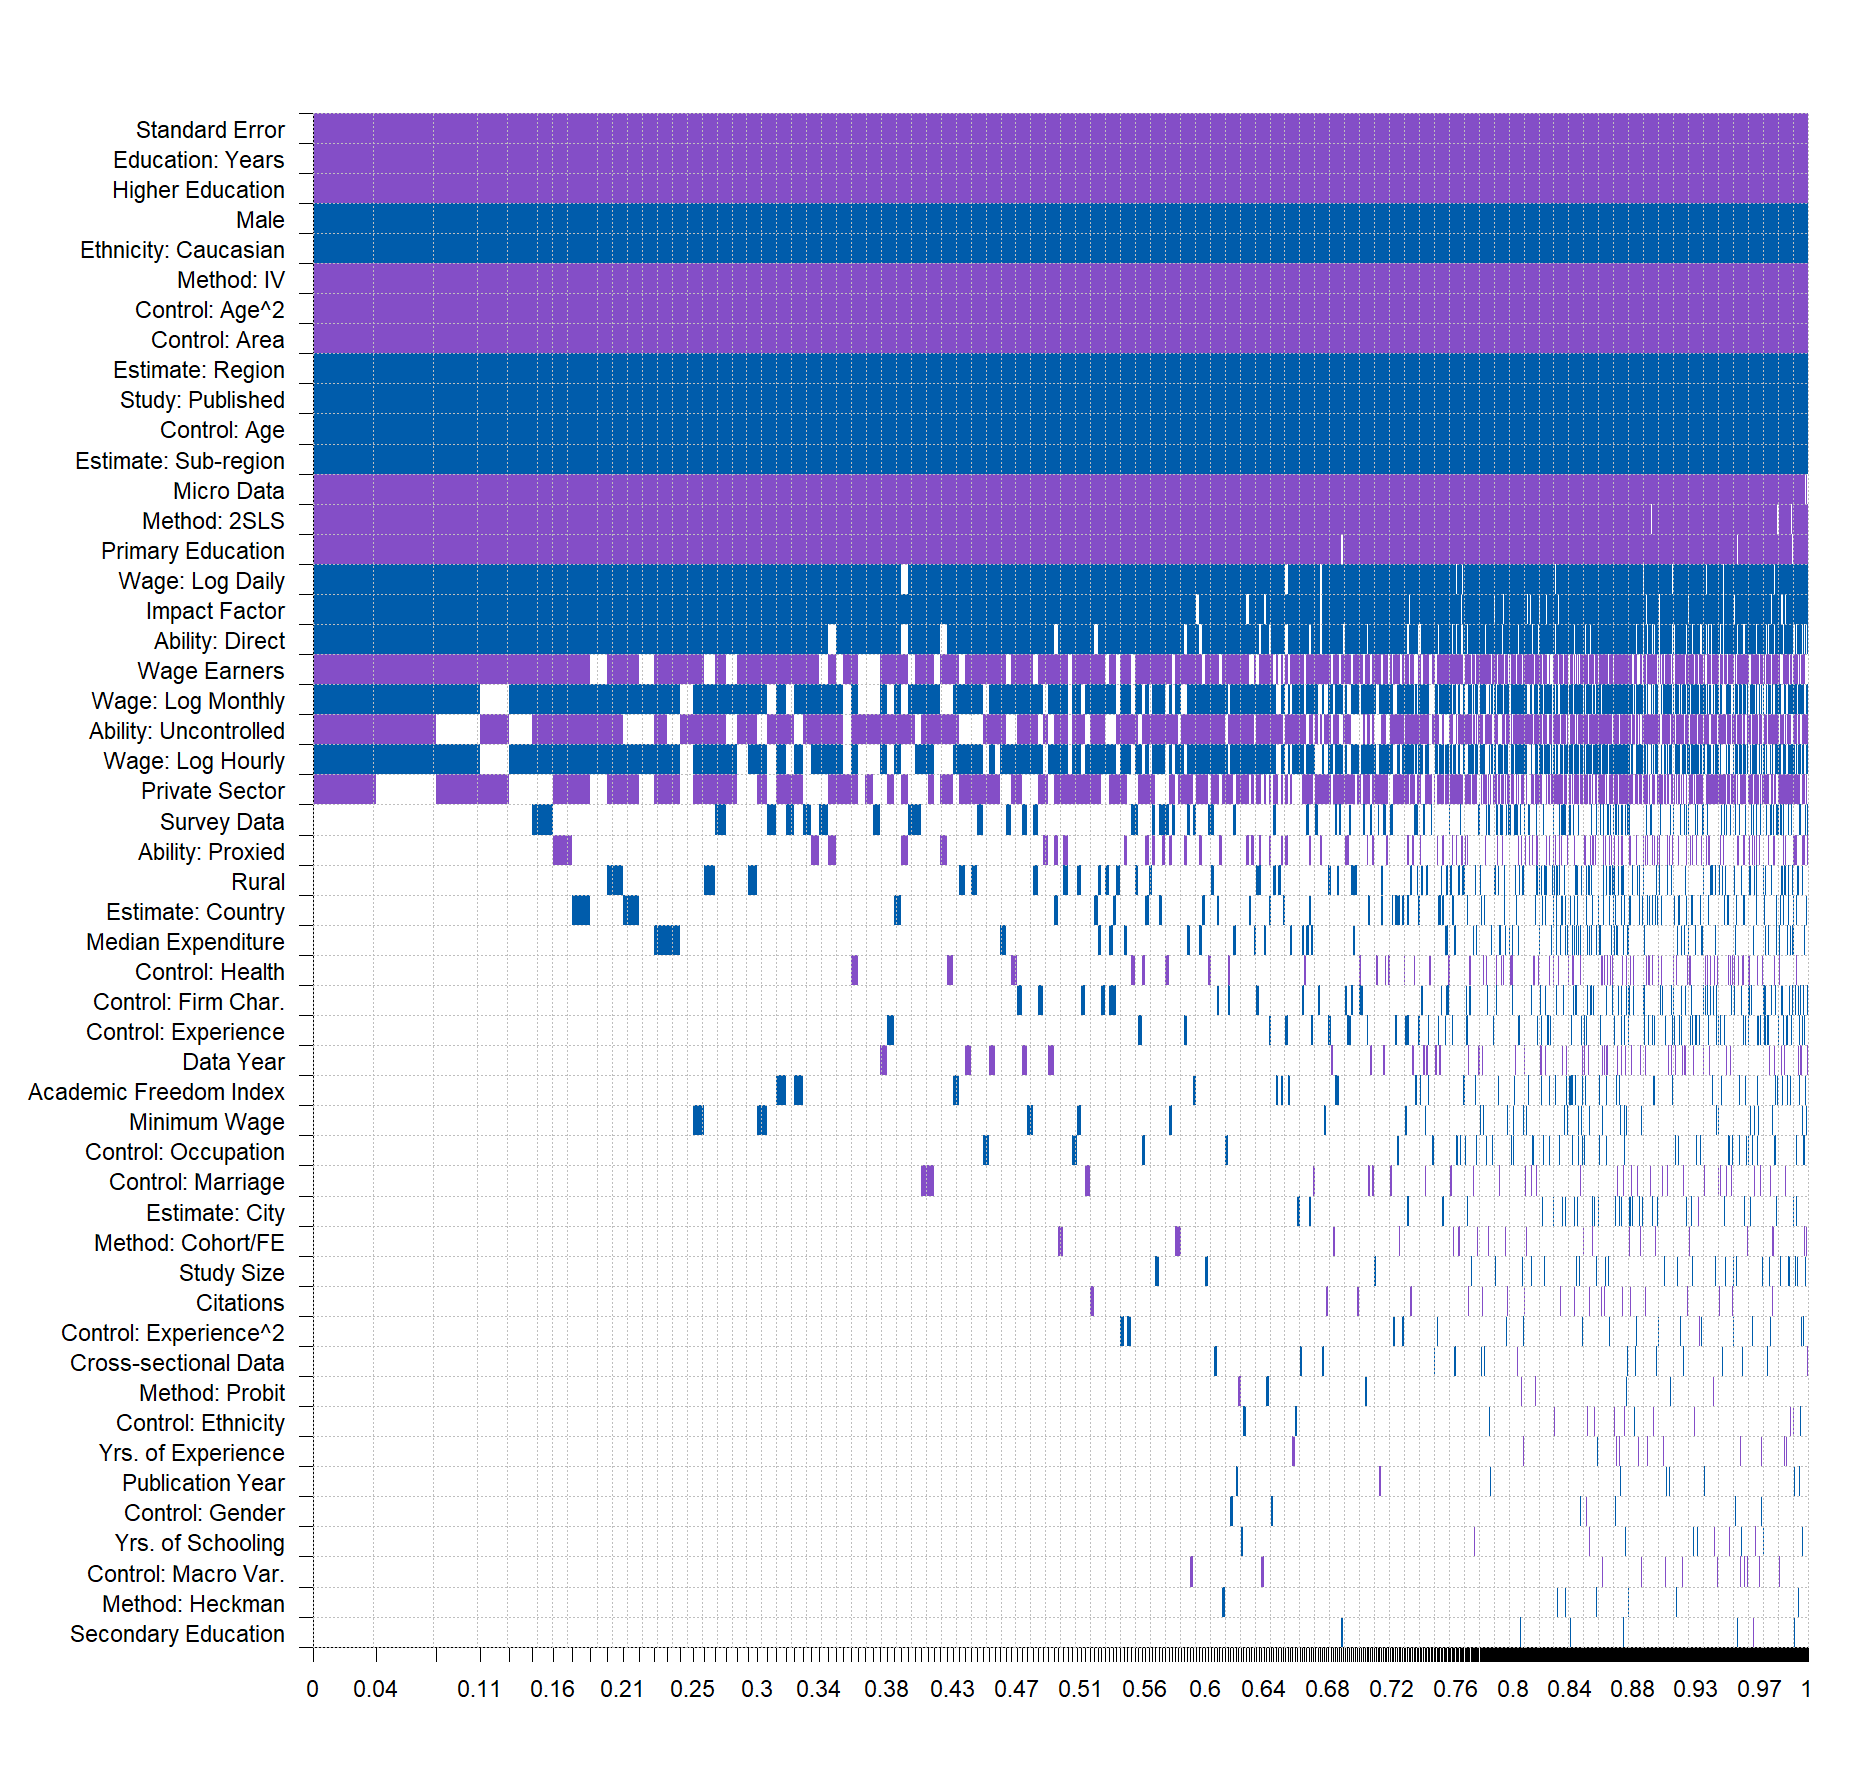
\includegraphics[width=0.9\textwidth]{Figures/BMA/bma_Hannan-Quinn_random_results.png}
\end{center}\vspace{-0.5cm}
\captionsetup{width=0.9\textwidth, font = scriptsize}
\caption*{\emph{Note:} This figure unveils the results of running the Bayesian model averaging using different specifications, namely the Hannan-Quinn criterion g-prior and the uniform model prior. BMA = Bayesian model averaging. HQ = Hannan-Quinn Criterion. For further explanation of the method and the employed variables, see \autoref{fig:BMA} and \autoref{tab:var}.
}
\end{figure}



\begin{figure}[!htbp]
\begin{center}
\caption{Bayesian Model Averaging - Correlation Table}
\label{fig:bma_corr}
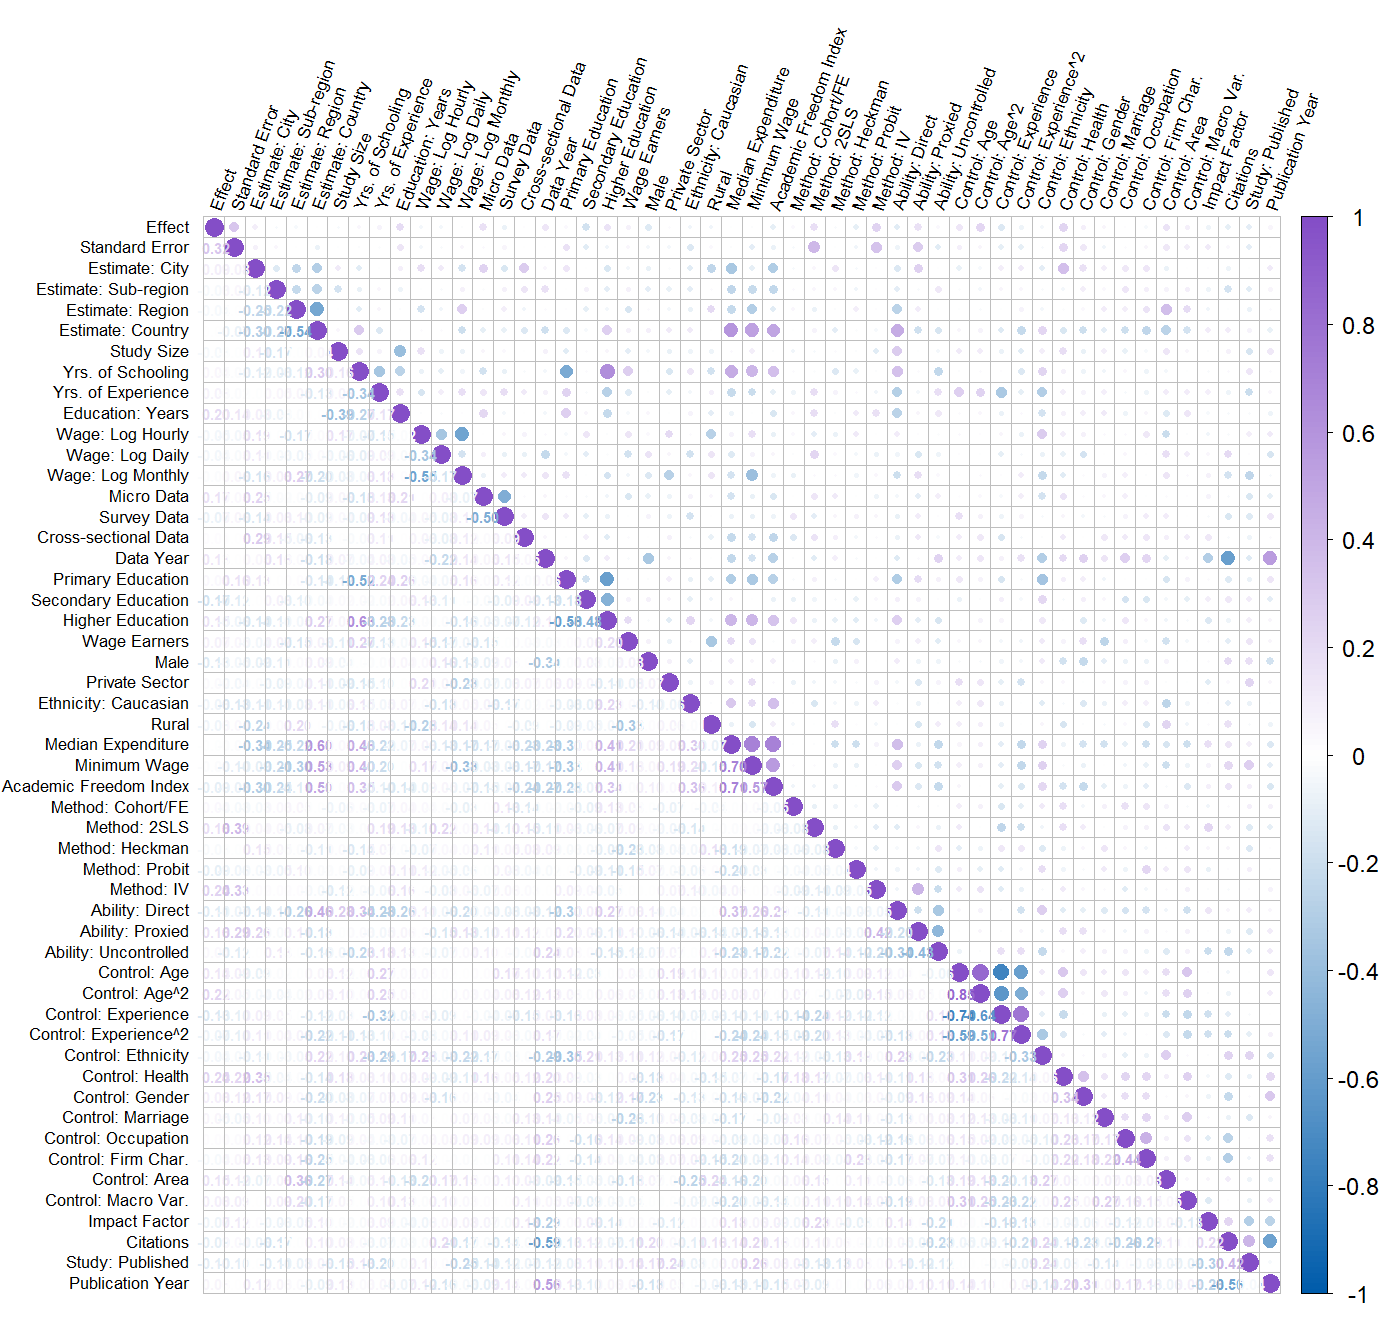
\includegraphics[width=1\textwidth]{Figures/BMA/bma_UIP_dilut_corrplot.png}
\end{center}\vspace{-0.5cm}
\captionsetup{width=0.9\textwidth, font = scriptsize}
\caption*{\emph{Note:} The figure shows the correlation between variables employed in the Bayesian model averaging. These variables are depicted on both axes. Purple color indicates a positive correlation; blue color indicates a negative correlation. Uniform g-prior and dilution model prior are used in the analysis. For results of the actual estimation, see \autoref{chap:five}. For a detailed explanation of the variables used, see \autoref{tab:var}.
}
\end{figure}




\chapter{Implied best-practice across literature}
\label{app:four}

\begin{singlespace}
\begin{footnotesize}
\begin{longtable}{
@{\hskip\tabcolsep}
l
*{2}{c}
@{}}
\caption{Comparing best-practice estimates across literature}  \label{tab:BPE_fun}\\
\toprule
    Study & Estimate & 95\% Confidence Interval \\
\midrule
\endfirsthead
\caption[]{Best-practice across literature (continued)}\\
\toprule
    Study & Estimate & 95\% Confidence Interval \\
\midrule
\endhead
\bottomrule
\multicolumn{3}{r}{{\scriptsize Continued on next page}} \\
\endfoot
\endlastfoot
           Author's subjective estimate &  6.849 &     (6.098; 7.6) \\
                                  \midrule
\multicolumn{3}{l}{\textit{Panel A: Studies identified by query (subset)}} \\
                            Leigh (2008) &  8.347 &   (6.838; 9.856) \\
                   Bartolj et al. (2013) &  8.117 &   (7.472; 8.762) \\
                    Salas-Velasco (2006) &  6.381 &   (5.209; 7.553) \\
      Lillo-Banuls \& Casado-Diaz (2010) &  7.000 &   (5.751; 8.249) \\
                       Wincenciak (2020) &  4.062 &   (2.839; 5.285) \\
                            Okuwa (2004) &  6.713 &    (5.19; 8.236) \\
                          Webbink (2004) & 10.158 &  (8.218; 12.098) \\
                     Kenayathulla (2013) &  9.194 &  (7.501; 10.887) \\
                        Asadullah (2006) &  5.781 &   (4.284; 7.278) \\
                         Maluccio (1998) &  9.221 &  (8.041; 10.401) \\
                    Depken et al. (2019) & 12.190 & (10.581; 13.799) \\
                Purnastuti et al. (2015) & 10.625 &  (8.594; 12.656) \\
                      Umar et al. (2014) &  8.514 &   (7.095; 9.933) \\
                          Sinning (2014) & 11.477 &  (10.43; 12.524) \\
                          Agrawal (2012) &  7.156 &   (5.729; 8.583) \\
                           Sackey (2008) &  6.196 &   (5.273; 7.119) \\
                  Patrinos et al. (2021) &  7.593 &   (6.301; 8.885) \\
                     Giles et al. (2019) &  6.597 &    (5.78; 7.414) \\
                   van der Hoeven (2013) &  7.747 &    (5.74; 9.754) \\
              Acemoglu \& Angrist (1999) &  6.546 &   (5.425; 7.667) \\
Vivatsurakit \& Vechbanyongratana (2020) & 10.587 &  (9.337; 11.837) \\
                              Qiu (2007) &  5.846 &     (4.792; 6.9) \\
                Mphuka \& Simumba (2012) & 12.434 &  (10.558; 14.31) \\
                            Aslam (2007) & 10.169 &  (8.521; 11.817) \\
               Himaz \& Aturupane (2016) &  8.043 &    (6.336; 9.75) \\
              Warunsiri \& McNown (2010) &  9.298 &  (7.583; 11.013) \\
                       Aromolaran (2006) &  6.633 &   (5.622; 7.644) \\
           Salehi-Isfahani et al. (2009) &  5.032 &    (4.03; 6.034) \\
                   Botchorishvili (2007) &  6.285 &   (5.013; 7.557) \\
                   Girma \& Kedir (2005) &  6.822 &   (4.727; 8.917) \\
              De Brauw \& Rozelle (2008) &  7.791 &   (6.394; 9.188) \\
                    Chanis et al. (2021) &  8.575 &  (7.132; 10.018) \\
  Paweenawat \& Vechbanyongratana (2015) & 10.628 &  (9.274; 11.982) \\
                   Vasudeva Dutta (2006) &  3.614 &   (2.144; 5.084) \\
                  Gibson \& Fatai (2006) &  6.318 &    (5.166; 7.47) \\
                           Hawley (2004) &  6.405 &   (5.074; 7.736) \\
                             Sohn (2013) &  9.375 &  (7.932; 10.818) \\
                    Harmon et al. (2002) & 10.018 &  (9.024; 11.012) \\
                            Lillo (2006) &  5.093 &   (4.137; 6.049) \\
                            Zhong (2011) &  8.776 &  (7.135; 10.417) \\
                           Krafft (2018) &  7.518 &    (5.57; 9.466) \\
                    Walker \& Zhu (2008) &  9.720 &  (8.722; 10.718) \\
                          Wambugu (2003) &  9.906 &  (7.789; 12.023) \\
                     Aryal et al. (2022) &  6.996 &   (5.593; 8.399) \\
                     Bakis et al. (2013) &  6.087 &   (5.336; 6.838) \\
               Campaniello et al. (2016) &  4.931 &   (3.604; 6.258) \\
                           Joseph (2020) &  9.501 &  (7.706; 11.296) \\
                          Dumauli (2015) & 10.443 &  (8.997; 11.889) \\
                 Fersterer et al. (2008) &  5.062 &    (3.28; 6.844) \\
                          Sinning (2017) & 11.524 & (10.372; 12.676) \\
                       Purnastuti (2013) &  4.965 &   (3.366; 6.564) \\
                            Arkes (2010) &  7.378 &   (6.151; 8.605) \\
                           Glewwe (1996) &  7.346 &   (5.298; 9.394) \\
                  Blundell et al. (2001) &  6.033 &    (4.636; 7.43) \\
                    Ayyash et al. (2020) &  8.716 &  (7.138; 10.294) \\ 
                     \midrule
\multicolumn{3}{l}{\textit{Panel B: Studies identified by snowballing}}\\
                    Aakvik et al. (2010) &  5.961 &   (4.683; 7.239) \\
                          Angrist (1995) &  7.419 &   (6.417; 8.421) \\
                   Angrist et al. (1991) &  8.807 &   (7.625; 9.989) \\
                    Belzil et al. (2002) &  5.943 &   (4.828; 7.058) \\
                         Brainerd (1998) &  2.465 &   (1.136; 3.794) \\
                            Breda (2014) &  0.884 &  (-0.494; 2.262) \\
                         Capatina (2014) &  6.357 &   (5.759; 6.955) \\
                             Card (1995) &  6.127 &   (5.031; 7.223) \\
                  Carneiro et al. (2011) &  6.852 &   (5.251; 8.453) \\
                            Chase (1998) &  3.115 &     (2.11; 4.12) \\
                  Devereux et al. (2010) &  6.210 &   (4.485; 7.935) \\
                 Dougherty et al. (1991) &  6.067 &   (4.677; 7.457) \\
                            Duflo (2001) &  7.471 &   (6.215; 8.727) \\
                        Duraisamy (2002) &  6.473 &   (5.785; 7.161) \\
                           Fortin (2008) &  4.105 &   (3.537; 4.673) \\
                      Gill et al. (2000) &  7.270 &   (6.486; 8.054) \\
                    Gorodnichenko (2005) &  4.944 &   (4.029; 5.859) \\
                   Grogger et al. (1995) &  3.367 &   (2.567; 4.167) \\
                    Harmon et al. (1995) & 10.136 &  (8.619; 11.653) \\
                    Harmon et al. (1999) &  9.261 &  (7.664; 10.858) \\
                    Harmon et al. (2003) &  7.878 &   (6.688; 9.068) \\
                   Heckman et al. (2006) &  8.440 &   (7.372; 9.508) \\
                          Hubbard (2011) &  7.005 &   (6.174; 7.836) \\
                           Ichino (1999) &  7.507 &   (6.123; 8.891) \\
                    Ichino et al. (2004) & 10.498 &  (8.981; 12.015) \\
                            Jones (2001) &  6.154 &   (4.512; 7.796) \\
                      Kane et al. (1993) &  6.584 &   (5.739; 7.429) \\
                           Kijima (2006) &  2.899 &   (2.039; 3.759) \\
                          Kingdon (1998) &  7.976 &   (6.553; 9.399) \\
                            Leigh (2008) &  8.277 &   (7.132; 9.422) \\
                   Lemieux et al. (2001) &  6.230 &   (5.321; 7.139) \\
                     Light et al. (2004) &  8.067 &   (7.001; 9.133) \\
                          Moretti (2004) &  6.581 &   (5.074; 8.088) \\
                    Munich et al. (2005) &  5.043 &   (3.653; 6.433) \\
                          Pischke (2005) &  6.801 &    (5.282; 8.32) \\
                   Psacharopoulos (1982) &  3.714 &    (2.318; 5.11) \\
                   Psacharopoulos (1979) &  7.461 &   (6.058; 8.864) \\
                   Staiger et al. (1997) &  7.507 &   (6.298; 8.716) \\
               Stephens Jr et al. (2014) &  6.126 &    (4.95; 7.302) \\
                            Taber (2001) &  6.277 &   (5.119; 7.435) \\
                           Troske (1999) &  3.728 &   (2.574; 4.882) \\
\bottomrule
\multicolumn{3}{>{\scriptsize}p{0.95\linewidth}}{\emph{Note:} The table reports estimates of the implied best-practice across studies of the main dataset, as well as the author's subjective best-practice. For clarity of presentation, I arbitrarily removed several query-identified studies from the table. 95\% confidence interval bounds are constructed as an approximate using OLS with study level clustered standard errors.}
\end{longtable}
\end{footnotesize}
\end{singlespace}
%\chapter{Twin dataset specifications}
\label{app:five}

% Possibly results from the twin dataset exploration here, if desired
\clearpage
%-----<<< --------- >>>-----


\end{document}
%-----<<<<<<<<< END OF DOCUMENT >>>>>>>>>-----



